\documentclass{./templates/mechthesis/MechThesis}
%
% Default options:
% [thesissizeG5,twoside,onecolumn,10pt,reqno,tbtags,globalpagenum,final]
%
%
% Available options:
% - size: [a4paper, letterpaper, thesissisze, thesissizeA4, thesissizeG5]
% - printing: [twoside, oneside]
% - columns: [onecolumn, twocolumns]
% - font size: [8pt, 9pt, 10pt, 11pt, 12pt]
% - position of equation numbers: [leqno, reqno]
% - split-equations numbers: [tbtags, centertags]
% - page numbers in papers: [globalpagenum, paperpagenum]
% - editing: [final, draft, printA4, cropmarks]
% - papers cover: [happyadvisor] (use it if you have more than 8 papers)
%
%
% Packages
%
% insert in this file any additional package
% Packages used in chapter open science
%\usepackage{epstopdf}
%\usepackage{listings}
%\usepackage{fancyref}

% \usepackage[newfloat,draft=true]{minted}
\usepackage[newfloat,finalizecache=true]{minted}
\usepackage{booktabs}
\usepackage{outlines}

%\usepackage{har2nat}


%% Uncomment the following
\usepackage{xspace}
% \usepackage[cmyk,dvipsnames]{xcolor}  % defined in MechThesis.cls
% \usepackage{sectsty}
\usepackage{enumitem}
% \usepackage{hyperref}
\usepackage{fancyhdr}
% \usepackage{titlesec}

\setlist[description]{leftmargin=1cm,labelindent=1cm}

%% Modify spacing
% \usepackage{setspace}
% \doublespacing

% The footnote package can save any footnotes entered inside a float and spit
% them out at the end (normally they are just thrown away, not sure why).
\usepackage{footnote}
\makesavenoteenv{figure}

\usepackage{braket}

%% Glossary
\usepackage[acronym,nonumberlist]{glossaries}
% \renewcommand*{\glsclearpage}{\clearpage}
% \usepackage{glossary-mcols}

% Packages used in chapter open science
%\usepackage{epstopdf}
%\usepackage{listings}
%\usepackage{fancyref}

% \usepackage[newfloat,draft=true]{minted}
\usepackage[newfloat,finalizecache=true]{minted}
\usepackage{booktabs}
\usepackage{outlines}

%\usepackage{har2nat}


%% Uncomment the following
\usepackage{xspace}
% \usepackage[cmyk,dvipsnames]{xcolor}  % defined in MechThesis.cls
% \usepackage{sectsty}
\usepackage{enumitem}
% \usepackage{hyperref}
\usepackage{fancyhdr}
% \usepackage{titlesec}

\setlist[description]{leftmargin=1cm,labelindent=1cm}

%% Modify spacing
% \usepackage{setspace}
% \doublespacing

% The footnote package can save any footnotes entered inside a float and spit
% them out at the end (normally they are just thrown away, not sure why).
\usepackage{footnote}
\makesavenoteenv{figure}

\usepackage{braket}

%% Glossary
\usepackage[acronym,nonumberlist]{glossaries}
% \renewcommand*{\glsclearpage}{\clearpage}
% \usepackage{glossary-mcols}

% Packages used in chapter open science
%\usepackage{epstopdf}
%\usepackage{listings}
%\usepackage{fancyref}

% \usepackage[newfloat,draft=true]{minted}
\usepackage[newfloat,finalizecache=true]{minted}
\usepackage{booktabs}
\usepackage{outlines}

%\usepackage{har2nat}


%% Uncomment the following
\usepackage{xspace}
% \usepackage[cmyk,dvipsnames]{xcolor}  % defined in MechThesis.cls
% \usepackage{sectsty}
\usepackage{enumitem}
% \usepackage{hyperref}
\usepackage{fancyhdr}
% \usepackage{titlesec}

\setlist[description]{leftmargin=1cm,labelindent=1cm}

%% Modify spacing
% \usepackage{setspace}
% \doublespacing

% The footnote package can save any footnotes entered inside a float and spit
% them out at the end (normally they are just thrown away, not sure why).
\usepackage{footnote}
\makesavenoteenv{figure}

\usepackage{braket}

%% Glossary
\usepackage[acronym,nonumberlist]{glossaries}
% \renewcommand*{\glsclearpage}{\clearpage}
% \usepackage{glossary-mcols}

\input{templates/mechthesis/packages}

% Insert HERE any additional packages
% \usepackage{graphicx} % Enhanced support for graphics

% Useful packages (not required):
%
% \usepackage{CJK} % CJK (Chinese, Japanese, Korean and Thai) language support
% \usepackage{listings} % Typeset source code listings using LaTeX
% \usepackage{longtable} % Allow tables to flow over page boundaries
% \usepackage{mathrsfs} % Support for using RSFS fonts in maths
% \usepackage{psfrag} % Replace strings in encapsulated PostScript figures
% \usepackage{rotating} % Rotation tools, including rotated full-page floats
% \usepackage{showframe} % Draw a page-layout diagram
% \usepackage[normalem]{ulem} % Package for underlining

%===============================================================================
%                        MechThesis includes the following
%===============================================================================
%
% The following packages are required by the MechThesis class
%
% \usepackage[utf8]{inputenc} % Accept different input encodings
% \usepackage[swedish,english]{babel} % Multilingual support for Plain TeX or LaTeX
% \usepackage{microtype} % Subliminal refinements towards typographical perfection
% \usepackage{csquotes} % Recommended for biblatex
% \usepackage[style=jfm,natbib=true]{biblatex}
% \usepackage{hyperref} % Extensive support for hypertext in LaTeX
% \usepackage{caption} % Correct figures and tables caption width
%
% The following packages are loaded by MechThesis.cls and need not to be loaded
% in this file:
% - color
% - amsmath
% - amsfonts
% - amssymb
% - amsthm
% - amsgen
% - crop        (if [printA4] or [cropmarks] options are used)
% - fp          (if [happyadvisor] option is used)

% Hyperref customizations

% Note: disable cmyk option in MechThesis.cls:362 to get true color
% \definecolor{hyperlinkcolor}{rgb}{0, 0, 1}  % blue
\definecolor{hyperlinkcolor}{cmyk}{1, 1, 0, 0}  % blue
% \definecolor{hyperlinkcolor}{rgb}{1, 0, 0}  % red
% \definecolor{hyperlinkcolor}{cmyk}{98, 52, 0, 0}  % KTH blue
% \definecolor{hyperlinkcolor}{HTML}{0645AD}  % Wikipedia blue
% \definecolor{hyperlinkcolor}{HTML}{0072CF}  % JFM blue: web

\hypersetup{
    bookmarks=true,         % show bookmarks bar?
    unicode=true,           % non-Latin characters in Acrobat’s bookmarks
    pdftoolbar=true,        % show Acrobat’s toolbar?
    pdfmenubar=true,        % show Acrobat’s menu?
    % pdffitwindow=true,     % window fit to page when opened
    % pdfstartview={FitH},   % fits the width of the page to the window
    pdftitle={Thesis - Advancements in stratified flows},    % title
    pdfauthor={Ashwin Vishnu Mohanan},     % author
    pdfsubject={Engineering Mechanics},   % subject of the document
    % pdfcreator={\author},   % creator of the document
    pdfproducer={KTH Royal Institute of Technology}, % producer of the document
    pdfkeywords={%
        geophysical flows, shallow water wave turbulence, energy cascade,%
        stratified turbulence, waves and vortices, open source software%
    },                      % list of keywords
    % pdfnewwindow=true,      % links in new PDF window
    % hidelinks,
    colorlinks=true,        % false: boxed links; true: colored links
    linktoc=all,            % link both the section names as well as the page number in toc
    % linktocpage=true,            % link just the page number in toc
    linkcolor=hyperlinkcolor,         % color of internal links (change box color with linkbordercolor)
    citecolor=hyperlinkcolor,         % color of links to bibliography
    filecolor=hyperlinkcolor,         % color of file links
    urlcolor=hyperlinkcolor,          % color of external links
}
\usepackage{subfig}
\usepackage{lmodern}


% Insert HERE any additional packages
% \usepackage{graphicx} % Enhanced support for graphics

% Useful packages (not required):
%
% \usepackage{CJK} % CJK (Chinese, Japanese, Korean and Thai) language support
% \usepackage{listings} % Typeset source code listings using LaTeX
% \usepackage{longtable} % Allow tables to flow over page boundaries
% \usepackage{mathrsfs} % Support for using RSFS fonts in maths
% \usepackage{psfrag} % Replace strings in encapsulated PostScript figures
% \usepackage{rotating} % Rotation tools, including rotated full-page floats
% \usepackage{showframe} % Draw a page-layout diagram
% \usepackage[normalem]{ulem} % Package for underlining

%===============================================================================
%                        MechThesis includes the following
%===============================================================================
%
% The following packages are required by the MechThesis class
%
% \usepackage[utf8]{inputenc} % Accept different input encodings
% \usepackage[swedish,english]{babel} % Multilingual support for Plain TeX or LaTeX
% \usepackage{microtype} % Subliminal refinements towards typographical perfection
% \usepackage{csquotes} % Recommended for biblatex
% \usepackage[style=jfm,natbib=true]{biblatex}
% \usepackage{hyperref} % Extensive support for hypertext in LaTeX
% \usepackage{caption} % Correct figures and tables caption width
%
% The following packages are loaded by MechThesis.cls and need not to be loaded
% in this file:
% - color
% - amsmath
% - amsfonts
% - amssymb
% - amsthm
% - amsgen
% - crop        (if [printA4] or [cropmarks] options are used)
% - fp          (if [happyadvisor] option is used)

% Hyperref customizations

% Note: disable cmyk option in MechThesis.cls:362 to get true color
% \definecolor{hyperlinkcolor}{rgb}{0, 0, 1}  % blue
\definecolor{hyperlinkcolor}{cmyk}{1, 1, 0, 0}  % blue
% \definecolor{hyperlinkcolor}{rgb}{1, 0, 0}  % red
% \definecolor{hyperlinkcolor}{cmyk}{98, 52, 0, 0}  % KTH blue
% \definecolor{hyperlinkcolor}{HTML}{0645AD}  % Wikipedia blue
% \definecolor{hyperlinkcolor}{HTML}{0072CF}  % JFM blue: web

\hypersetup{
    bookmarks=true,         % show bookmarks bar?
    unicode=true,           % non-Latin characters in Acrobat’s bookmarks
    pdftoolbar=true,        % show Acrobat’s toolbar?
    pdfmenubar=true,        % show Acrobat’s menu?
    % pdffitwindow=true,     % window fit to page when opened
    % pdfstartview={FitH},   % fits the width of the page to the window
    pdftitle={Thesis - Advancements in stratified flows},    % title
    pdfauthor={Ashwin Vishnu Mohanan},     % author
    pdfsubject={Engineering Mechanics},   % subject of the document
    % pdfcreator={\author},   % creator of the document
    pdfproducer={KTH Royal Institute of Technology}, % producer of the document
    pdfkeywords={%
        geophysical flows, shallow water wave turbulence, energy cascade,%
        stratified turbulence, waves and vortices, open source software%
    },                      % list of keywords
    % pdfnewwindow=true,      % links in new PDF window
    % hidelinks,
    colorlinks=true,        % false: boxed links; true: colored links
    linktoc=all,            % link both the section names as well as the page number in toc
    % linktocpage=true,            % link just the page number in toc
    linkcolor=hyperlinkcolor,         % color of internal links (change box color with linkbordercolor)
    citecolor=hyperlinkcolor,         % color of links to bibliography
    filecolor=hyperlinkcolor,         % color of file links
    urlcolor=hyperlinkcolor,          % color of external links
}
\usepackage{subfig}
\usepackage{lmodern}


% Insert HERE any additional packages
% \usepackage{graphicx} % Enhanced support for graphics

% Useful packages (not required):
%
% \usepackage{CJK} % CJK (Chinese, Japanese, Korean and Thai) language support
% \usepackage{listings} % Typeset source code listings using LaTeX
% \usepackage{longtable} % Allow tables to flow over page boundaries
% \usepackage{mathrsfs} % Support for using RSFS fonts in maths
% \usepackage{psfrag} % Replace strings in encapsulated PostScript figures
% \usepackage{rotating} % Rotation tools, including rotated full-page floats
% \usepackage{showframe} % Draw a page-layout diagram
% \usepackage[normalem]{ulem} % Package for underlining

%===============================================================================
%                        MechThesis includes the following
%===============================================================================
%
% The following packages are required by the MechThesis class
%
% \usepackage[utf8]{inputenc} % Accept different input encodings
% \usepackage[swedish,english]{babel} % Multilingual support for Plain TeX or LaTeX
% \usepackage{microtype} % Subliminal refinements towards typographical perfection
% \usepackage{csquotes} % Recommended for biblatex
% \usepackage[style=jfm,natbib=true]{biblatex}
% \usepackage{hyperref} % Extensive support for hypertext in LaTeX
% \usepackage{caption} % Correct figures and tables caption width
%
% The following packages are loaded by MechThesis.cls and need not to be loaded
% in this file:
% - color
% - amsmath
% - amsfonts
% - amssymb
% - amsthm
% - amsgen
% - crop        (if [printA4] or [cropmarks] options are used)
% - fp          (if [happyadvisor] option is used)

% Hyperref customizations

% Note: disable cmyk option in MechThesis.cls:362 to get true color
% \definecolor{hyperlinkcolor}{rgb}{0, 0, 1}  % blue
\definecolor{hyperlinkcolor}{cmyk}{1, 1, 0, 0}  % blue
% \definecolor{hyperlinkcolor}{rgb}{1, 0, 0}  % red
% \definecolor{hyperlinkcolor}{cmyk}{98, 52, 0, 0}  % KTH blue
% \definecolor{hyperlinkcolor}{HTML}{0645AD}  % Wikipedia blue
% \definecolor{hyperlinkcolor}{HTML}{0072CF}  % JFM blue: web

\hypersetup{
    bookmarks=true,         % show bookmarks bar?
    unicode=true,           % non-Latin characters in Acrobat’s bookmarks
    pdftoolbar=true,        % show Acrobat’s toolbar?
    pdfmenubar=true,        % show Acrobat’s menu?
    % pdffitwindow=true,     % window fit to page when opened
    % pdfstartview={FitH},   % fits the width of the page to the window
    pdftitle={Thesis - Advancements in stratified flows},    % title
    pdfauthor={Ashwin Vishnu Mohanan},     % author
    pdfsubject={Engineering Mechanics},   % subject of the document
    % pdfcreator={\author},   % creator of the document
    pdfproducer={KTH Royal Institute of Technology}, % producer of the document
    pdfkeywords={%
        geophysical flows, shallow water wave turbulence, energy cascade,%
        stratified turbulence, waves and vortices, open source software%
    },                      % list of keywords
    % pdfnewwindow=true,      % links in new PDF window
    % hidelinks,
    colorlinks=true,        % false: boxed links; true: colored links
    linktoc=all,            % link both the section names as well as the page number in toc
    % linktocpage=true,            % link just the page number in toc
    linkcolor=hyperlinkcolor,         % color of internal links (change box color with linkbordercolor)
    citecolor=hyperlinkcolor,         % color of links to bibliography
    filecolor=hyperlinkcolor,         % color of file links
    urlcolor=hyperlinkcolor,          % color of external links
}
\usepackage{subfig}
\usepackage{lmodern}

%
%
% Commands
%
% insert in this file any additional command
% Pandoc preamble
\PassOptionsToPackage{unicode}{hyperref}
\PassOptionsToPackage{hyphens}{url}
%
% \usepackage{lmodern}
% \usepackage{amssymb,amsmath}
% \usepackage{ifxetex,ifluatex}
% \ifnum 0\ifxetex 1\fi\ifluatex 1\fi=0 % if pdftex
%   \usepackage[T1]{fontenc}
%   \usepackage[utf8]{inputenc}
%   \usepackage{textcomp} % provide euro and other symbols
% \else % if luatex or xetex
%   \usepackage{unicode-math}
%   \defaultfontfeatures{Scale=MatchLowercase}
%   \defaultfontfeatures[\rmfamily]{Ligatures=TeX,Scale=1}
% \fi
% % Use upquote if available, for straight quotes in verbatim environments
% \IfFileExists{upquote.sty}{\usepackage{upquote}}{}
% \IfFileExists{microtype.sty}{% use microtype if available
%   \usepackage[]{microtype}
%   \UseMicrotypeSet[protrusion]{basicmath} % disable protrusion for tt fonts
% }{}
% \makeatletter
% \@ifundefined{KOMAClassName}{% if non-KOMA class
%   \IfFileExists{parskip.sty}{%
%     \usepackage{parskip}
%   }{% else
%     \setlength{\parindent}{0pt}
%     \setlength{\parskip}{6pt plus 2pt minus 1pt}}
% }{% if KOMA class
%   \KOMAoptions{parskip=half}}
% \makeatother
% \usepackage{xcolor}
\IfFileExists{xurl.sty}{\usepackage{xurl}}{} % add URL line breaks if available
% \IfFileExists{bookmark.sty}{\usepackage{bookmark}}{\usepackage{hyperref}}
% \hypersetup{
%   hidelinks,
%   pdfcreator={LaTeX via pandoc}}
% \urlstyle{same} % disable monospaced font for URLs
\usepackage{graphicx,grffile}

\makeatletter
\def\maxwidth{\ifdim\Gin@nat@width>\linewidth\linewidth\else\Gin@nat@width\fi}
\def\maxheight{\ifdim\Gin@nat@height>\textheight\textheight\else\Gin@nat@height\fi}
\makeatother

% Scale images if necessary, so that they will not overflow the page
% margins by default, and it is still possible to overwrite the defaults
% using explicit options in \includegraphics[width, height, ...]{}
\setkeys{Gin}{width=\maxwidth,height=\maxheight,keepaspectratio}

% Set default figure placement to htbp
\makeatletter
\def\fps@figure{htbp}
\makeatother

\setlength{\emergencystretch}{3em} % prevent overfull lines

\providecommand{\tightlist}{%
  \setlength{\itemsep}{0pt}\setlength{\parskip}{0pt}}

% \setcounter{secnumdepth}{-\maxdimen} % remove section numbering

% \makeatletter
% \@ifpackageloaded{subfig}{}{\usepackage{subfig}}
% \@ifpackageloaded{caption}{}{\usepackage{caption}}
% \captionsetup[subfloat]{margin=0.5em}
% \AtBeginDocument{%
% \renewcommand*\figurename{Figure}
% \renewcommand*\tablename{Table}
% }
% \AtBeginDocument{%
% \renewcommand*\listfigurename{List of Figures}
% \renewcommand*\listtablename{List of Tables}
% }
% \@ifpackageloaded{float}{}{\usepackage{float}}
% \floatstyle{ruled}
% \@ifundefined{c@chapter}{\newfloat{codelisting}{h}{lop}}{\newfloat{codelisting}{h}{lop}[chapter]}
% \floatname{codelisting}{Listing}
% \newcommand*\listoflistings{\listof{codelisting}{List of Listings}}
% \makeatother


% % Insert HERE any additional commands


% as examples here are some commands from the JFM template:
%
\newcommand\etal{\mbox{\textit{et al.}}}
\newcommand\etc{etc.\ }
\newcommand\eg{e.g.\ }

\providecommand\bnabla{\boldsymbol{\nabla}}
\providecommand\bcdot{\boldsymbol{\cdot}}

\newcommand\Rey{\mbox{\textit{Re}}}  % Reynolds number
\newcommand\Pran{\mbox{\textit{Pr}}} % Prandtl number, cf TeX's \Pr product
\newcommand\Pen{\mbox{\textit{Pe}}}  % Peclet number


% Commands used for chapter open science
\newcommand{\fluidpack}[1]{\href{https://fluid#1.readthedocs.io}{%
\codeinline{fluid#1}}}

% \newcommand{\codeinline}[1]{\mintinline{python}{#1}}
\newcommand{\codeinline}[1]{\texttt{#1}}

\newcommand{\fluiddyn}{\fluidpack{dyn}\xspace}

\newcommand{\Numpy}{\codeinline{Numpy}\xspace}
\newcommand{\Scipy}{\codeinline{Scipy}\xspace}

\newcommand{\pack}[1]{\codeinline{#1}\xspace}

\newcommand{\mako}{\href{http://www.makotemplates.org/}{\pack{mako}}}

\newcommand{\libpack}[2][]{%
  \ifstrequal{#2}{FFTW}{%
    \href{http://fftw.org}{#2}}{%
  \ifstrequal{#2}{MKL}{%
    \href{https://software.intel.com/en-us/mkl}{#2}}{%
  \ifstrequal{#2}{PFFT}{%
    \href{https://www-user.tu-chemnitz.de/~potts/workgroup/pippig/software.php.en}{#2}}{%
  \ifstrequal{#2}{P3DFFT}{%
    \href{http://p3dfft.net}{#2}}{%
  \ifstrequal{#2}{2decomp\&FFT}{%
    \href{http://www.2decomp.org}{#2}}{%
  \ifstrequal{#2}{cuFFT}{%
    \href{https://docs.nvidia.com/cuda/cufft/index.html}{#2}}{%
  \ifstrequal{#2}{clFFT}{%
    \href{https://clmathlibraries.github.io/clFFT/}{#2}}{%
  \ifstrequal{#2}{FFTPACK}{%
    \href{http://www.netlib.org/fftpack}{#2}}{%
  \ifstrempty{#1}{%
    #2
  }{%
    \href{#1}{#2}}
  }}}}}}}}\xspace  % Close the if-else-if tree above!
}


% other
\newcommand{\p}{\partial}
\newcommand{\Dt}[1]{\ensuremath{\frac{D #1}{Dt}}}

% Wikipedia-style "citation needed" macro
\newcommand{\citationneeded}[1][]{\textsuperscript{\color{blue} [citation needed: #1]}}

\newcommand{\paragraphbf}[1]{\subparagraph{\bf #1}}

\renewcommand{\descriptionlabel}[1]{\hspace{\labelsep}\textit{#1}}

% Extend href with footnote url
\newcommand{\fnref}[3][]{\href{#2}{#3}\footnote{#1\url{#2}}}

% !Undefined control sequence.
% https://tex.stackexchange.com/questions/8361/latex-ieeetran-cls-use-titlesec-package
% \newcommand{\tocsubparagraph}{}

% commands from milestone_issf paper
\newcommand{\R}{\mathcal{R}}

\newcommand{\eps}{\varepsilon}
\newcommand{\epsK}{\varepsilon_{\!\scriptscriptstyle K}}
\newcommand{\epsA}{\varepsilon_{\!\scriptscriptstyle A}}
% From shallow water paper
\newcommand\shalf{\ensuremath{{\scriptstyle\frac{1}{2}}}}
\newcommand\sh{\ensuremath{^{\shalf}}}
\newcommand\smh{\ensuremath{^{-\shalf}}}
\newcommand\squart{\ensuremath{{\textstyle\frac{1}{4}}}}
\newcommand\thalf{\ensuremath{{\textstyle\frac{1}{2}}}}
\newcommand\Gat{\ensuremath{\widetilde{G_a}}}
\newcommand\ttz{\ensuremath{\rightarrow 0}}
\newcommand\ndq{\ensuremath{\frac{\mbox{$\partial$}}{\mbox{$\partial$} n_q}}}
\newcommand\sumjm{\ensuremath{\sum_{j=1}^{M}}}
\newcommand\pvi{\ensuremath{\int_0^{\infty}%
  \mskip \ifCUPmtlplainloaded -30mu\else -33mu\fi -\quad}}


\newcommand{\uu}{\textbf{u}}
\newcommand{\xx}{\textbf{x}}
\newcommand{\kk}{\textbf{k}}
\newcommand{\JJ}{\textbf{J}}
\newcommand{\rr}{\textbf{r}}
\newcommand{\ff}{\textbf{f}}
\newcommand{\FF}{\textbf{F}}
\newcommand{\baa}{\textbf{a}}
\newcommand{\bb}{\textbf{b}}
\newcommand{\NN}{\textbf{N}}





\newcommand{\ErtelPV}{\mathcal{Q}}

\newcommand{\fdiss}{f_{\mbox{\scriptsize diss}}}

\newcommand{\D}{\mbox{D}}

\newcommand{\eez}{\boldsymbol{e_z}}
\newcommand{\scalarprod}[2]{\big( #1 \, , \ #2 \big)_{\kk}}

\newcommand{\mean}[1]{\langle #1 \rangle}

\newcommand{\meane}[1]{\langle #1 \rangle}
% \newcommand{\meane}[1]{{\langle #1 \rangle_{\hspace{-0.4mm}e}}}

\newcommand{\meanx}[1]{{\langle #1 \rangle_{\hspace{-0.4mm}\mbox{\scriptsize$\xx$}}}}

\newcommand{\meant}[1]{{\langle #1 \rangle_{\hspace{-0.4mm}\theta}}}

\newcommand{\means}[1]{{\langle #1 \rangle_{\hspace{-0.4mm}s}}}

\newcommand{\shocks}{ {\mbox{\tiny shocks}} }

\newcommand{\kmax}{k_{\mbox{\scriptsize max}}}
\newcommand{\kdiss}{k_{\mbox{\scriptsize diss}}}


\newcommand{\mA}{\mathcal{A}}


\newlength{\halfwidth}
\setlength{\halfwidth}{2.6in}

\newcommand{\PA}[1]{{\color{green}#1}}

\newcommand{\Add}[1]{{\color{blue}#1}}
% \newcommand{\Add}[1]{#1}
\newcommand{\Remove}[1]{{\color{red}\st{#1}}}
% \newcommand{\Remove}[1]{}

\newtheorem{lemma}{Lemma}
\newtheorem{corollary}{Corollary}

% Milestone paper
\newcommand{\vv}{\boldsymbol{v}}
\newcommand{\CKA}{C_{K\rightarrow A}}
\newlength{\figwidth}
\setlength{\figwidth}{0.7\textwidth}

% Personal
\newcommand{\order}[1]{\ensuremath{\mathcal{O}(#1)}}
\newcommand{\kfivethird}{\ensuremath{k^{-5/3}}}
\newcommand{\pder}[2][]{\frac{\partial#1}{\partial#2}}

\DeclareOldFontCommand{\bf}{\normalfont\bfseries}{\mathbf}

\newcommand{\red}[1]{{\color{red}{#1}}}
\newcommand{\green}[1]{{\color{teal}{#1}}}



%-------------------------------------------------------------------------------
% Thesis information
%-------------------------------------------------------------------------------
%
\title[%
  Advancements in stratified flows through simulation, experiment and open research software development%
]% Title used in the abstract (optional)
{% Title of the thesis
  Advancements in stratified flows through \\ simulation, experiment and \\ open
  research software development%
}%

\author{Ashwin Vishnu Mohanan}% Author

\affiliation
{%	Author's affiliation
	Department of Mechanics, KTH Royal Institute of Technology,\\
	SE--100 44 Stockholm, Sweden%
}%

\titel
{% Swedish title (for swedish abstract)
  Framsteg inom stratifierade str\"omningar genom simulering, experiment och
  utveckling av \"oppen mjukvara
}%

\anslutning
{% Author's swedish affiliation (for swedish abstract)
    Institutionen f\"or Mekanik, Kungliga Tekniska h\"ogskolan,\\
	SE-100 44 Stockholm, Sverige%
}%

%TODO: verify details of publishing info, defence etc
\date{Stockholm}{{August}}{{2019}}% City, Month, Year

\info{% Defence information (in swedish)
	Akademisk avhandling som med tillst\aa nd av Kungliga Tekniska H\"{o}gskolan
	i Stockholm framl\"{a}gges till offentlig granskning f\"{o}r avl\"{a}ggande
	av teknologie
	doktorsexamen % doktorsexamen/licentiatsexamen
	{fredagen den 27 september 2019 kl 10:00} % day (no capital initials on days and month)
	i sal {F3}, % room
	Kungliga Tekniska H\"{o}gskolan, Lindstedtsvägen 26, Stockholm.% address
	%
	\\[\baselineskip]% TODO: Publishing info
	%
	TRITA-SCI-FOU \change{3641:01}\\ % you get from Stefan or Vivi or Daniel: skult@mech.kth.se - vivi@mech.kth.se - danse@kth.se
	ISBN \change{978-91-7942-634-9} % you get from KTH library: https://www.kth.se/en/kthb/publicering/kths-publikationsdat/bestallning-av-isbn-1.535558
	%
	% there are no more ISSN nor ISRN
	%
	\\[\baselineskip]% Cover info (comment if no cover image is used)
	%
    {\it Cover:} collage of flow visualization from simulations and experiments.
	%
	% In case you are interested
	% the colour of the blue ribbon at the bottom of the page is:
	% PANTONE 2935 U  https://www.pantone.com/color-finder/2935-U
	% which corresponds to:
	% RGB      27 95 170
	% CMYK     98 52 0 0
	% HEX/HTML 1B5FAA
	%
	% you can find more info about printing and the graphics at the following pages
	% https://www.kth.se/en/kthb/publicering/kths-publikationsdat/for-forskare/spikningen-steg-for-steg-1.584638
	% https://www.kth.se/en/student/program/examensarbete/avhandlingarochexamensarbeten/avhandlingar-och-examensarbeten-1.458230
	% https://www.kth.se/polopoly_fs/1.477580!/KTH%20Inlaga_avhandling_stylesheet.pdf
}%

\printer{Universitetsservice US--AB, Stockholm}% Printer informations

\bibliography{thesis}

%===============================================================================
%===============================================================================
%                            BEGIN DOCUMENT
%===============================================================================
%===============================================================================

% \includeonly{overview}
% \includeonly{paper_06_milestone/paper}
% \includeonly{paper_03_toy_model/paper,paper_04_shallow_water/paper}
% \includeonly{paper_04_shallow_water/paper}

\input{glossary}

\begin{document}


%===============================================================================
% Frontmatter
%===============================================================================
%
\frontmatter

%-------------------------------------------------------------------------------
% Cover page
%-------------------------------------------------------------------------------
%
\makecoverpage


%-------------------------------------------------------------------------------
% Dedication (comment if none)
%-------------------------------------------------------------------------------
%
\dedication{
	% {\it ``You must unlearn what you have learnt.''}\\[20pt]
	% Master Yoda
	{\it ``Essentially, all models are wrong, but some are useful.''}\\[20pt]
	George E.~P.~Box
}


%-------------------------------------------------------------------------------
% Abstract (English)
%-------------------------------------------------------------------------------
%
% COMMENT: the abstract should be limited to 2000 characters and the keywords
% to 250 characters because otherwise they will not fit in the mailing sheet.
%
% TODO: abstract in english and swedish
\begin{abstract}
    \noindent%
Two studies of two-dimensional models of flows influenced by stratification and stratification/rotation are carried out in
order to investigate whether a two-dimensional model can reproduce a downscale energy cascade with an associated $ k^{-5/3} $ wavenumber  spectrum.
 Firstly, a series of highly resolved numerical simulations of the classical shallow water model is carried out. A forward energy cascade is observed but the dynamics is dominated by shocks, with an associated $ k^{-2} $-spectrum.
A theory for shallow water wave turbulence is formulated and compared to the results from the simulations.
 Secondly, a series of simulations of a new two-dimensional toy model is carried out, showing that  the model is not generating  shocks and can reproduce a downscale energy cascade with
an associated $ k^{-5/3} $ spectrum. The energy transfer is studied in detail in Fourier space and is compared with results from a general circulation model.

An experimental study of strongly stratified turbulence at the Coriolis platform in Grenoble is carried out, with the aim of testing novel theories of stratified turbulence. Turbulence is generated by traversing an array of cylinders through a tank containing stratified salt water. Velocity is measured by Particle Image Velocimetry (PIV) and density is measured by conductivity probes. In particular, the author has developed the software system analysing the PIV images. Preliminary results from the experiment are presented.

 To realise the research objectives, a set of open-source software packages are developed in Python, under the
umbrella of the FluidDyn project. The
packages enable execution of simulations, experiments and processing of data.
The codes are well documented, tested and designed to
promote development and reuse.

\keywords{geophysical flows, shallow water wave turbulence, energy cascade,
stratified turbulence, waves and vortices, open source software}

	% Access points  must work. In fact, few cryptographers would disagree with
	% the emulation of robots, which embodies the technical principles of
	% complexity theory. Hyp, our new application for lossless information, is the
	% solution to all of these challenges.
	%         %
	%         \keywords{super-lasers, space-stations, The Force, cookies.}
	%         %
\end{abstract}


%-------------------------------------------------------------------------------
% Abstrakt (Swedish)
%-------------------------------------------------------------------------------
%
% COMMENT: the abstract should be limited to 2000 characters and the keywords
% to 250 characters because otherwise they will not fit in the mailing sheet.
%
\begin{abstrakt}
    \noindent%
Tv\aa $ \; $  studier av tv\aa dimensionella modeller av str\"omningar
influerade av stratifiering respektive stratifiering och rotation genomf\"ors,
i syfte att unders\"oka huruvida en {tv\aa}dimensionell modell kan reproducera en energikaskad till mindre skalor med ett associerat v\aa gtalsspektrum av formen $ k^{-5/3} $.  F\"orst genomf\"ors en serie h\"oguppl\"osta simuleringar av den klassiska modellen f\"or str\"omningar i grunt vatten (shallow water model). En energikaskad till mindre skalor observeras, men str\"omningen domineras av st\"otar med ett associerat $ k^{-2} $-spektrum.
Sedan genomf\"ors en serie simuleringar av en ny tv\aa dimensionell leksaksmodell, som visar att modellen kan reproducera en energikaskad till mindre skalor med ett associerat $ k^{-5/3}$-spektrum. Energi\"overf\"oringen studeras i detalj i Fourier-rummet och j\"amf\"ors med resultat fr\aa n en global cirkulationsmodell.


En experimentell studie av starkt stratifierad turbulens genomf\"ors vid Coriolisplattformen i Grenoble, med m\aa let att testa nya teorier f\"or stratifierad turbulens. Turbulensen genereras genom att traversera en rad cylindrar genom en tank inneh\aa llande stratifierat saltvatten. Hastighet m\"ats med Particle Image Velocimetry (PIV) och densitet m\"ats med konduktivitetssonder. I synnerhet har f\"orfattaren utvecklat den programvara som analyserar bilder fr\aa n PIV-m\"atningarna. Prelimin\"ara resultat fr\aa n experimentet presenteras.

F\"or att realisera forskningsm\aa len  utvecklas en m\"angd mjukvarupaket f\"or \"oppet bruk i Python, i ett projekt med namnet FluidDyn. Paketen erbjuder m\"ojligheter att utf\"ora simuleringar, experiment och databehandling. Koderna \"ar v\"al dokumenterade, testade och designade f\"or att underl\"atta utveckling och \aa teranv\"andning.

\nyckelord{geofysikaliska str\"omningar, v\aa gturbulens i grunt vatten,
stratifierad turbulens, v\aa gor och virvlar, \"oppen mjukvara}

	% \r{A}tkomstpunkter m\r{a}ste arbeta. I sj\"{a}lva verket skulle f\r{a}
	% kryptografer h\r{a}ller inte med emulering av robotar, som
	% f\"{o}rkroppsligar de tekniska principer av komplexitetsteori. Hyp, v\r{a}r
	% nya applikation f\"{o}r f\"{o}rlustfri information är l\"{o}sningen på alla
	% dessa utmaningar.
	%         %
	%         \nyckelord{super-lasrar, rymdstationer, Kraften, kakor.}
	%         %
\end{abstrakt}


%-------------------------------------------------------------------------------
% Preface page
%-------------------------------------------------------------------------------
%
\begin{preface}
    This thesis contains numerical, theoretical, experimental and
    technical studies aiming at advancing the understanding of stratified flows.
    Studies which motivated this thesis, along with theoretical
    details and research highlights of the present work are summarized in the
    first part. The second part contains five articles and one conference
    paper.
    The papers are adjusted to comply with the present thesis format for
    consistency, but their contents have not been altered as compared with their
    original counterparts.
\end{preface}


%-------------------------------------------------------------------------------
% Division of work between authors
%-------------------------------------------------------------------------------
%
\begin{divisionofwork}
	The main advisor for the thesis is Erik Lindborg (EL).
    Pierre Augier (PA) acts as co-advisor.

	\paperitem
        The code was developed by PA and Ashwin Vishnu
        Mohanan (AVM). The simulations and post-processing were performed
        by AVM. The theory was developed by PA and EL with input from AVM. A
        first version of the paper was written by PA. The final version was
        written by EL with input from AVM.
        %
	\paperitem
        The code development, the simulations and post-processing was
        handled by AVM. The paper was written by EL with input from
        AVM.
        %
    \paperitem
        The experiment was planned by the group from KTH together with the group from
        LEGI. The experimental set-up was put together by
        the group from LEGI. The experiment was carried out by the two groups
        together.
        The code for image-processing was developed by AVM, PA, Antoine
        Campagne (AC), Joel Sommeria (JS) and the code for processing
        probe data was developed by PA, RC and Diane Micard. The
        post-processing was performed by AVM, PA, AC, AS and JS.
        The paper was written by AC with input from PA, EL and AVM.
        %
    \paperitem
        The code was developed by PA, Cyrille Bonamy (CB) and AVM. The paper
        was authored by PA with input from AVM.
    \paperitem
        The code was developed by AVM, CB and PA.
        The code was benchmarked for performance by PA and AVM.
        The paper was written by AVM with inputs from PA and CB.
    \paperitem
        The code was developed by AVM, CB, Miguel Calpe Linares (MCL) and PA.
        The code was benchmarked for performance by PA and AVM.
        The paper was written by AVM with inputs from PA and CB.

\end{divisionofwork}


%TODO: fill in additional publications and conferences
%-------------------------------------------------------------------------------
% Additional publications (comment if none)
%-------------------------------------------------------------------------------
%
% \begin{otherpublications}
%         The following papers, although related, are not included in this thesis.
%
%   \paperitem%
%     {Anakin Skywalker \& Master Obi-Wan Kenobi}% Authors
%     {3639}% Year
%     {The light sabre: an elegant weapon for a more civilized age}% Title
%     {Jedi Journal of Weapons}% Journal
%     {33}% Volume
%     {2}% Number
%     {pp. 55--60}% Pages
%
% \end{otherpublications}


%-------------------------------------------------------------------------------
% Conferences (comment if none)
%-------------------------------------------------------------------------------
%
% \begin{conferences}
%         Part of the work in this thesis has been presented at the following
%         international conferences. The presenting author is underlined.
%
%   \conferenceitem%
%     {Anakin Skywalker, \underline{Darth Vader} \& Admiral Motti}% Authors
%     {3639}% Year
%     {Effects on breathing of underestimation of the power of The Force}% Title
%     {Intergalactic Conference on Weapons and Peace}% Conference
%     {Kamino}% Location
%
% \end{conferences}


%-------------------------------------------------------------------------------
% Table of contents
%-------------------------------------------------------------------------------
%
\tableofcontents


\printglossary

%===============================================================================
% Part I: Overview and summary
%===============================================================================
%
\mainmatter


\part{Overview and summary}

%-------------------------------------------------------------------------------
% Overview and summary
%
\begin{refsection}
  \graphicspath{{imgs/}}

%===============================================================================
% ALL CHAPTERS GO HERE
%===============================================================================
\input{chapter_00_0_intro.latex}
\input{chapter_00_1_swe_decomp.latex}
\input{chapter_00_2_toy_model.latex}
\input{chapter_00_3_budget.latex}
\input{chapter_00_4_results.latex}
\input{chapter_01_0_intro.latex}
\input{chapter_01_1_exp_desc.latex}
\input{chapter_01_2_exp_contrib.latex}
\input{chapter_01_3_exp_results.latex}
% \chapter{Towards reproducible, open science through open research software}
\section{Introduction}


% FIXME: Deleted
% Science: giants, collective, grows when shared
% Web: money, open-source, tools esp. DVCS
% Computing: performance, GPU
% Changes: dynamics, way science is done, coding inferior, open science

% see http://sciencecodemanifesto.org/
% http://lorenabarba.com/gallery/reproducibility-pi-manifesto/
% https://www.numfocus.org/
%
% http://www.nature.com/news/interactive-notebooks-sharing-the-code-1.16261
% We provide examples of solutions for: Good coding practice, source control
% management, packaging, licenses documentation, testing,CI

% Fluiddyn: foster open-science, source. Framework for collaborative dev, open
% methods

In order to attain the research goals in this thesis, a path off the beaten
track was pursued -- i.e. to create a handful of easy to maintain, rigorously
tested, and most-importantly, open-source scientific packages which do not
compromise on performance.
%
This resulted in the creation of FluidDyn, a project to facilitate open-science
in the field of fluid mechanics.
%
The focus of the project was to develop a set of packages to implement a
framework for simulations \citep{fluidsim}, experiments
\citep{augier_fluidimage_2016,augier_fluidlab_nodate}, Fast Fourier Transforms
\citep{fluidfft} -- all depending on a base package to reuse certain utilities
and data structures \citep{fluiddyn}.
%
The project owes a lot to the recent developments in methods and tools for
open-source software engineering.
%
Several modern coding practices were adopted while developing these packages.


The FluidDyn packages are primarily written in Python language. Incidentally,
it is the defining characteristics of Python which make the eventual success of
such a project realizable.
%
Python is one of the most important tools in recent open-source dynamics,
particularly in science.
%
The popularity of the language in fluid mechanics is growing, but Python is yet
to reach widespread adoption as the language of choice.

We shall now discuss these topics in greater detail. The chapter is organized
into four sections. The first section focusses on the technical aspects, with
particular focus on emerging developments in programming languages, tools and
services suited for open-source software development. The subsequent section
presents Python's strengths and weaknesses as a language for scientific
computing.
%
The third section compares various software development methodologies. Here, we
will also discuss about the possible contradiction between productivity of
individuals and productivity at the community level.
%
The chapter finally ends with a summary of the motivations for the project
FluidDyn and an overview of the packages we have developed.
% The chapter ends with a note on the capabilities of FluidDyn
% packages\footnote{We use FluidDyn (with capital letters) to name the project
% and \fluiddyn for the base package.}.
%

% \section{Science, software, open-source and the computer revolution}
\section{Open-source software and open-science}

Computational sciences, and especially computational fluid dynamics (CFD) as a
discipline, have flourished in the latter half of the twentieth century.
Incidentally, the origin of this discipline can be traced back to the ideas in
\citet{richardson_weather_1922} to achieve numerical weather prediction.
Following the arrival of first electronic general-purpose computer, ENIAC in
1945, the first simulations were made by \citet{charney_numerical_1950} using a
simple barotropic model to make 24 hour forecasts \citep[see
also][]{lynch_richardson_2010}. In those early days when the availability of
computers was limited, such methods were neither widespread nor feasible.
Scientific investigations were dominated by theoretical and experimental
methods.
%
We have come a long way and today computational methods complement theoretical
and experimental studies, and are equally important.
%
% Thus, in a typical scientific study, there is significant effort involved in
% translating the mathematical representation to a working research software.
%
With the connectivity provided by the world wide web it is possible to achieve
more and reinvent the way we do sciences.

\begin{figure}[h]
  \centering
  \includegraphics[width=0.8\textwidth]{open_science}
  \caption{A schematic representation of various concepts and methodologies
  involved in achieving reproducibility in sciences.}\label{fig:opensci}
\end{figure}

In recent years, there has been a move towards open science
\citep[see the report by][]{royal_society_great_britain_science_2012}.
%
Depicted in figure~\ref{fig:opensci} are some of steps needed to ensure
reproducibility and transparency in sciences.
%
Traditionally, \emph{knowledge} has been disseminated in the form of courses
and books from universities, and to the wider scientific community through
research articles, conference proceedings and workshops.
%
In the last decade, knowledge has become more accessible to the public
through public-domain and Creative Commons (or similar) licensed course
materials and massively open online courses (MOOCs). Moreover, there is also an
emerging push to publish in open-access journals\footnote{In the European
  Union, a proposal to implement Plan S (\url{https://www.coalition-s.org}) was
  been set in motion in September 2018 to fast track adoption of open-access.
} either through systematic
reforms in academia on how researchers' productivity are assessed, or through
regulations and offering incentives, such as waiving the application processing
charge for publishing \citep{nosek_promoting_2015}.

A lot of work is required to condense and implement this knowledge in the form
of working applications.
%
The \emph{know-how} can be made accessible and open to scrutiny by making
research software open-source with an appropriate license\footnote{For a
	detailed comparison of licenses, visit either
	\url{https://choosealicense.com} or
	\url{https://www.gnu.org/licenses/license-list.html}. }.
%
To make codes usable they have to be complemented by documentation which
typically includes tutorials, examples and a detailed commentary of different
components.
%
Furthermore, to inspire confidence in and to ensure reliability of a code
throughout the process of software development, it needs unit-tests through
which it is continuously built, tested and deployed --- a process known as
Continuous Integration (CI). Depending on how matured a software is, CI can be
easy or cumbersome to implement, but nevertheless, the result is a cleaner and
reliable code.

Finally, the \emph{results} generated from such codes together with the
workflow (i.e.\ scripts to run the codes and to post-process the data) when made
open in the form of datasets can ensure that research is reproducible and
preserved in archives for several years to come \citep{gewin_data_2016}. Open
datasets can be shared and made citable through services such as
\href{https://zenodo.org}{Zenodo} and \href{https://figshare.com}{Figshare}.

In FluidDyn project, we have strived to implement all the aspects of making the
know-how open through open-source software. We shall now take a look at the
tools which have made it possible.

\subsection{Methods and tools for open-source software engineering}

\subsubsection{Free and Open-Source Software}

The Free and Open-Source Software (FOSS) movement has given rise to the tools
that enable open-source software development today.
%
The term \emph{free} in FOSS is a misnomer, as it actually stands for
\emph{freedom} (to use, modify and distribute). The FOSS movement has
dramatically decreased the cost of using computers, which is evident from the
widespread use of GNU/Linux systems in desktops, computing clusters and
web-servers in academia and beyond.
%
The FOSS culture can be traced back to the success of typesetting
standards \TeX\ (1977) and \LaTeX\ (1985) for authoring scientific publications.
%
Another founding moment for the FOSS movement was the launch of the GNU project
in 1983 by \href{https://en.wikipedia.org/wiki/Richard_Stallman}{Richard
  Stallman}, to create a Unix-like computer operating system composed entirely
  of free software\footnote{For completeness, see also the work done on
  \href{https://www.levenez.com/unix/}{other Unix operating systems, for
example BSD}.}.
%
GNU is today known for its compiler collection (GCC) and a multitude of tools
which combined with the Linux kernel (created by
\href{https://en.wikipedia.org/wiki/Linus_Torvalds}{Linus Torvalds} in 1991)
forms the GNU/Linux operating system
% and its several distributions (Debian, Red Hat, Slackware, Arch Linux and
% Gentoo to name a few)
that we are familiar with today.
%
% FOSS movement has had huge successes in many frontiers --- Apache could be
% termed as the ``first killer-app of Linux'' and now with an ever-increasing
% suite of softwares including Firefox, LibreOffice, Gimp as solid alternatives
% to proprietary offerings.
%
Linux has become the most widely used kernel, being deployed on servers,
personal computers, embedded devices, and also smart phones (with Android). The
success of the Linux kernel project was attributed to the \emph{bazaar} model of
software development, as described in \citet{raymond_cathedral_1999}, wherein a
code can stay structured despite releasing frequently and delegating tasks to
community with myriad agendas.

% remark Julien Salort: not interesting. Nothing on BSD.
% https://www.levenez.com/unix/

Over the years, FOSS development has transitioned from an organic community of
volunteers, towards an organized system with participation from industries,
non-profit organizations and government institutions.
%
Such a model results in a win-win scenario -- users benefit from transparency and
ability to tinker, and the organizations profit with more contributions.
%
The FOSS movement has now entered into a second era
\citep{fitzgerald_transformation_2006}.

% - 90s arrival of internet (soon mass market)

% Some huge open-source successes : Apache ("first killer app of Linux"),
% now Firefox, Open-office
% av: https://www.reddit.com/r/AskReddit/comments/7x639l/what_free_software_is_so_good_you_cant_believe/du6pw11/

% Linux kernel now widely used on servers, personal computers, embedded
% devices, smarth phone (with Android).
% https://en.wikipedia.org/wiki/Linux_kernel

% Now, new period for open-source:
% see http://www.cepis.org/upgrade/files/full-2005-III.pdf

% - "Libre Software Movement: The Next Evolution of The IT Production
% Organization?"

% - ``the composition of development teams was changing, from all-volunteer
% teams to teams with paid participants from industry, government or
% not-for-profit organizations.''

% By the way, we also have to use the term "libre software" (?)
% av: Libre-software is not so mainstream. Even Linux kernel is not libre with
% binary blobs for drivers.

% We may have to change the order of this list?
% - git and mercurial 2005
% - software repositories ~ 10 years before
% so I would exchange the too paragraph...
% av:That is probably because we did not mention patches and CVS, subversion
% etc.

\subsubsection{Source code management}

Collaboration was achieved in the early years of FOSS development through
emailing ``patches'', and centralized Version Control Systems (VCS) near the
turn of the 21\textsuperscript{st} century.  The collective collaboration on
development is today streamlined with the emergence of Distributed Version
Control Systems (DVCS), especially, Git and Mercurial).
%
Version control tools are designed to work on any kind of text files, not just
codes, so they could even be utilized to write scientific documents with
multiple authors.
%
In web-based source development platforms like GitHub, Bitbucket and GitLab,
DVCS repositories are enhanced with code-review tools, typically consisting of
a issue tracker and pull-request mechanism.
%
Git has become the \textit{de facto} standard for source management. However,
for the FluidDyn project, we prefer to use Mercurial because we consider it to
be simpler for the beginners and just as powerful for expert users\footnote{See
  \href{https://www.mercurial-scm.org/wiki/GitConcepts}{``a detailed
comparison''} on Mercurial website.}. Simplicity and low learning barriers for
scientists who are not experts in software development is crucial for our
project.
%
Note that, it is now possible to use Mercurial to work with Git repositories,
for example hosted in GitHub and GitLab\footnote{By using the Mercurial
extension \href{http://hg-git.github.io/}{hg-git}.}.
%
The use of DVCS in science will lead to long term productivity benefits
\citep{wilson_best_2014}.


\subsubsection{Package management and software repositories}

Packaging process depends on the language used in a project, however some good
practices are universal, such as licensing, supplying documentation (a README
file at the bare minimum), keeping installation paths flexible and relying on
official build tools \citep{taschuk_ten_2017}.
%
A credible repository to packages as compressed archives or as pre-compiled binary
packages is indispensable to promote code reuse and reproducibility of results.
%
The use of repositories started with the conception of
CPAN and CRAN repositories for the languages Perl and R in 1993 --- based on
the Comprehensive \TeX\ Archive Network (CTAN) model for \TeX\ packages.
%
Python as a medium for scientific computing owes its success to a rich
ecosystem of third-party packages. \href{https://pypi.org}{Python Package
Index (PyPI)} and \href{https://anaconda.org}{Anaconda Cloud} are major
repositories for delivering and downloading Python packages, assisted by
package managers \pack{pip} and \pack{conda} respectively. The
\fnref{https://packaging.python.org}{``Python Packaging User Guide''} is an
excellent guide to learn how to install, package and distribute projects.
% Almost all major
% languages\footnote{\href{https://stackoverflow.com/questions/1693529/%
% list-of-top-repositories-by-programming-language}{https://stackoverflow.com/%
% questions/1693529/list-of-top-repositories-by-programming-language}} have
% similar repositories, with exceptions such as Fortran and Matlab.
Specialized package managers, such as \pack{easybuild} and \pack{spack}, have
also emerged to install scientific libraries and compilers.

\subsubsection{Continuous Integration and documentation} The need for
strong reliability of packages with increasing complexity has forced developers
to use Continuous Integration (CI).
%
When the code depends on a wide variety of external dependencies, CI is useful
to avoid \fnref{https://en.wikipedia.org/wiki/Software\_rot}{software rot},
i.e.\ to avoid obsolescence with newer versions of the compiler or its
dependencies. CI is specifically important for dynamical languages and
open-source code since, it allows open-source projects to welcome contributions
from other developers while maintaining a high degree of reliability.
%
Firstly, the code is \emph{built} against a known, repeatable emulation
environment on a server. Thereafter, a set of \emph{unit tests} are run for
each commit (modification of the code) to check that no bugs have been
introduced. It is also important to analyse what portion of the source code is
covered by these unit tests --- a method referred to as \emph{code coverage}.
%
Almost all CI platforms are free for open-source projects --- Travis CI,
CircleCI and Appveyor to name a few. Bitbucket and GitLab have built-in CI
implementations. Websites such as Codecov and Coveralls help to chart and
analyse the code coverage history, viewable by anyone. To use these services,
one simply has to write a simple file in YAML format and authenticate the
respective services with ``read'' permissions.

New users and developers often rely on good documentation and examples.
Documentation generators such as Sphinx (for Python) and Doxygen (for many
languages including C, C++, Fortran and Python) parses in-line comments into
documentations as PDF, HTML and more \citep{lee_ten_2018}.
%
The documentation generation can be automated online and deployed using any CI.
``Read the Docs'' has, in recent years, become the hub for building and hosting
documentation online, thus facilitating the process for developers and
considerably improving access to information for users.
%
In the FluidDyn project we this limit ourselves to automating tests and
documentation of the latest version. It is possible to further exploit the
CI by adding code style checks by running ``linters'' alongside unit tests,
\emph{continuous delivery} of package releases and preserving older versions of
documentation.

\subsubsection{Knowledge hubs and communication}

% Mutual aid and knowledge sharing have been important aspects of the web since
% its inception and these practices are now of foremost importance for many
% human activities.
%
%In particular,
Learning programming and computer science is now greatly aided by websites like
the community driven encyclopaedia \href{https://www.wikipedia.org/}{Wikipedia}
or the community driven forum \href{https://stackoverflow.com/}{Stack
Overflow}, where people write thousands of questions and answers on programming
each week. The IRC protocol has continued to sustain the test of time. Instant
messaging channels such as \codeinline{\#python} on Freenode facilitate
interactive discussions and a form of community-level support system --- a role
which used to be filled by mailing lists alone in the past. Alternatives such
as Riot (Matrix protocol), Gitter, and Slack have gained popularity offering
different integration solutions on top of instant messaging.
%
Through instant messaging a geographically separated team, as in the case of
the FluidDyn project, can achieve near real-time collaboration without having
to arrange video conferences or meetings.

Thus, there is a number of new methods and tools in software development.
Taken all together, they greatly improve our collective efficiency and
open possibilities for interactions that were unthinkable a few years ago.
%
For example, the success of community-driven software like \pack{astropy} (a
subject-area research library with
\href{https://github.com/astropy/astropy}{more than 240 contributors}) and
\pack{scikit-learn} (a machine learning toolkit with
\href{https://github.com/scikit-learn/scikit-learn}{more than 1000
contributors}) would not have been possible without these new software
development methods.
%
As scientists, we can wonder how to fully exploit these new possibilities to do
science. The project FluidDyn is an attempt to advance the fluid dynamics
community in this direction.


\section{Python, a programming language adapted for open-science}

We now turn to the presentation of the
\href{https://www.python.org/}{programming language Python}, another
fundamental tool for the FluidDyn project. Note that, this is not a detailed
technical presentation: we focus on the ideas necessary to understand why the
FluidDyn project is based on this language and on facts interesting for
potential FluidDyn users and developers.

The Python community has thrived remarkably in the last few years, which is
evident from the fact that by the end of 2017, Python became the second most
popular language in terms of pull-requests in GitHub\footnote{%
%See GitHub's annual report titled \href
\url{https://octoverse.github.com/2017}
% { ``The State of the Octoverse 2017''}.
%
} and
\fnref%
% [See the blog post ``The Incredible Growth of Python'']%
{https://stackoverflow.blog/2017/09/06/incredible-growth-python/}%
{questions on StackOverflow}.
%
TIOBE-index\footnote{\url{https://www.tiobe.com/tiobe-index}}, which assess the
popularity of a language based on number of skilled users, courses and
third-party vendors, ranks Python at number four. IEEE Spectrum\footnote{
%See the analysis titled
\url{https://spectrum.ieee.org/computing/software/the-2017-top-programming-languages}
%{``The 2017 Top Programming Languages''} on IEEE spectrum.
}
ranks Python as the most popular language in 2017 with a metric
based on trends, demand by employers and users on open-source hubs.  All the
rankings agree that Python usage has been steadily growing and is here to stay.
Python largely outclasses languages like Fortran and Matlab according to these
statistics, and is now clearly one of the mainstream languages with C, Java,
C++ and JavaScript.
%
The language has been designed to boost the communication of technical ideas
between humans.
%
Let us summarize some characteristics of the Python languages that have lead to
such an incredible success.
%
Python differs from other mainstream languages for a variety of reasons:


\begin{itemize}
\item \textbf{Aesthetics.} The syntax is expressive, with an inherent emphasis
on readability. Blocks of code are defined with the indentation.

\item \textbf{Code style.} There are official (but, optional) guidelines, named
\fnref{https://www.python.org/dev/peps/pep-0008/}{PEP~8}, advocating for
regularity of the code. Linters and code-formatters can evaluate and enforce
adherence to this style.

\item \textbf{Automatic memory management.}  A garbage collector handles the
memory allocation and deallocation, which needs no user intervention. There
are, of course, ways to control the memory usage of a program, though not as
precisely as for low-level languages.

\item \textbf{Dynamic typing.}
The types of objects are inferred at run time from the code and the
context, and in many situations, one does not need to declare them explicitly.

\item \textbf{Interpreted.} The standard way\footnote{There are also tools to
compile Python code (for example Cython and Pythran).} to run a Python code is
to ``interpret'' it.  A program called the interpreter executes the code
nearly\footnote{Actually, the execution of Python code is less simple and
involves an Abstract Syntax Tree.} instruction-by-instruction, with very few
optimizations.
%
In contrast to other compiled languages, such as Fortran, C or C++, there is no
proper compilation step: the code is not translated to optimized machine
instructions, but only to Python bytecode.

\item \textbf{Multi-paradigm.} Imperative, object-oriented, functional
and aspect-oriented programming are supported.

\item \textbf{Extensible}. It is easy to interface with code written in
several other languages (in particular C, C++ and Fortran).

\item \textbf{Batteries included.} Python comes with a large
\fnref{https://docs.python.org/3/library/index.html}{standard library}.

\item \textbf{Cross platform.} Python can be deployed on many different
machines with different operating systems (Linux, Windows, macOS, Android) and
architectures (from a microcontroller --- with MicroPython or CircuitPython ---
to a Blue Gene supercomputer).

\end{itemize}
%
Thus, Python is one of the best ``glue'' languages for fast prototyping.
Code development in Python is much faster and easier than with many other
languages. Less bugs are introduced by the developers simply because there are
fewer lines of code \citep{nanz_comparative_2015}.
%
Maintaining and modifying existing code is also facilitated by the very good code
readability associated with the language.
%
Another consequence of the apparent simplicity of Python is that the learning
curve has a nice shape. Learning Python is very easy from the start and the
complexity gradually increases as the level of the developer increases.
%
Its interpreted nature is advantageous for a rapid development cycle and the
possibility of interactive workflow (usually with IPython or Jupyter
notebooks).
%
Therefore, Python is good for developers at all levels: very gentle for
beginners and very powerful for advanced users.

Python is an old language (first implementation in 1991!) but it continues to
evolve.
%
Note that there are many implementations of Python
interpreters\footnote{Notable ones are CPython (written in C), Jython (Java),
IronPython (C\#), PyPy (Rpython, a subset of Python) and
MicroPython/CircuitPython (C, targeted to micro-controllers).}. The default and
most widely used implementation is written in C and is called CPython.
%
A hard and controversial decision was taken to clean up Python from its
historical incoherences by introducing a new series of backwards-incompatible
versions of the language, starting with Python 3.0, released in December 2008.
After a long and difficult process, the transition from Python 2 to Python 3 is
completed for nearly all important packages\footnote{Close to
\href{https://python3wos.appspot.com/}{95\% of the most downloaded packages}
are Python 3 compatible as of 2018.}. Especially for scientific applications,
we can now work only in Python 3. For instance, \href{https://github.com/%
numpy/numpy/blob/master/doc/neps/dropping-python2.7-proposal.rst}{future
versions of \Numpy} and \fnref{http://www.python3statement.org/}{the main
scientific packages} will not be compatible with Python 2. These changes
open doors to a very clean, coherent and potentially faster Python
experience. Therefore, one should not use Python 2 for science any more and
instead, adopt the newer versions.
%
New versions of Python have nice features to adapt to new usages and to
recent trends in computer science.  For example, three new features were
introduced in Python 3.5 (first released on September 2015): the \codeinline{@}
operator for matrix multiplication, the new \codeinline{async} and
\codeinline{await} keywords for concurrency and type hinting\footnote{See also our
paragraph on the issue of type checking in the following.} (with the module
\codeinline{typing} and an associated syntax presented in the
\href{https://www.python.org/dev/peps/pep-0484/}{PEP~484}).

Being a very versatile language, Python is widely used for many different
applications\footnote{\href{https://www.jetbrains.com/research/devecosystem-2018/python/}{See
\emph{The State of Developer Ecosystem Survey in 2018} by JetBrains}}:

\begin{itemize}
\item Simple scripting

\item Web development

\item Data science

\item System, database and network administration

\item GNU/Linux distribution software

\item GUI desktop applications

\item Scripting layer for applications (for example Paraview, Visit, QGIS,
	Blender)

\item Web scraping

\item Animation, gaming and film industry

\item Education

\item Science

\end{itemize}
%
Python
% has recently become one of the most popular language for teaching programming
% and developing scientific applications. It
has now a mature and powerful scientific ecosystem with well-established
foundational packages
%
(\Numpy for N-dimensional homogeneous arrays, \Scipy as the
fundamental toolkit for scientific computing, \pack{Matplotlib} for plotting
and \pack{Pandas} for data structures) and several more specialized packages
(to name a few, \pack{h5py}, \pack{mpi4py}, \pack{skimage}, \pack{sklearn}).
The \href{https://github.com/rougier/python-visualization-landscape}{%
landscape of visualization tools usable through Python} makes it possible to
integrate post-processing and analysis capabilities into a single application.
%
Python is one of the main languages for data science with packages such as
\pack{Pandas}, \pack{statmodels}, \pack{sklearn}, \pack{Keras},
\pack{TensorFlow} and \pack{PyTorch}.
%
There are user-friendly and ready-to-use Python installers (similar to Matlab), in
particular the
\href{https://en.wikipedia.org/wiki/Anaconda_(Python_distribution)}{%
open-source distribution Anaconda} to streamline the installation in
desktop platforms.
Integrated development environments (IDE) adapted for
scientists, for example \href{https://github.com/spyder-ide/spyder}{Spyder},
\href{https://pyzo.org}{Pyzo},
and \href{https://jupyterlab.readthedocs.io}{JupyterLab} are often useful for
interactive development.

Python has a very large and supportive community (see, for example,
\fnref{http://stackoverflow.com/tags/python}{Stack Overflow tags}).
%
Python development is also supported by companies, and most of them specialize
in web technologies and data-driven research. However, recently, companies
involved in scientific software development have started to become quite
influential. For example, Anaconda Inc.\ is strongly engaged in the development
of tools like JIT Python accelerator \pack{Numba}, and parallelism framework
\pack{dask}. Hardware giants such as Intel and Nvidia also contribute to the
Python scientific ecosystem.
%
To summarize, Python's numerous features and its adoption in several domains
makes it a sensible language choice for scientific purposes.

\subsection{Some Python issues and their solutions}

In the context of scientific computing there are some common issues that Python
developers would face. The issues are listed below and the solutions are
specified briefly. The solutions are explained in further detail in subsequent
paragraphs.

\begin{itemize}

\item \textbf{Performance in CPU bounded tasks.} Since the standard Python
	interpreter does not do any proper compilation, pure Python code for
	some CPU bounded tasks can be too slow. Thus, one has to avoid writing
	loops as much as possible and use vectorized array operations as much
	as possible. One can also call \emph{foreign functions}, or use special
	tools to build extensions using \emph{Ahead Of Time} or \emph{Just In
	Time} compilation to speedup performance-critical code.

\item \textbf{Absence of type checking.} In contrast to compiled languages,
	there is no type-checking in Python (and more generally in many
	interpreted languages). Types are respected however, and type errors,
	if any, would be raised during runtime.
	\emph{Type hints} and \emph{static type checking} can solve this issue.

\item \textbf{Concurrent, but not parallel multi-threading.} Threads behave
	like light sub-programs. In principle, they can use the different cores
	of the CPU at the same time, but the CPython interpreter forbid threads
	to interpret python code at the same time\footnote{See
	\url{https://opensource.com/article/17/4/grok-gil}
	%{a blog article ``How to grok the GIL''}
	% and \url{https://faster-cpython.readthedocs.io/cpython37.html}{a
	% technical presentation by a CPython core developer}.
	}. In other words, threads can coexist concurrently, by not executing in
	parallel.
%
This limitation comes from an important detail in the implementation of the
CPython interpreter: a Global Interpreter Lock (GIL) to prevent race conditions
that could corrupt data.
%
GIL greatly simplifies the implementation of CPython and that
it is very difficult to remove it while keeping other nice technical properties
of CPython intact\footnote{See
\url{https://wiki.python.org/moin/GlobalInterpreterLock}. Note that PyPy
also uses a GIL, while two other implementations of the Python language, Jython
and IronPython, do not have this limitation}.

\item \textbf{Lively, and thus, complicated ecosystem of packages.} For many
	applications, the standard library is insufficient and external
	packages are needed. Sometimes there are multiple options and the
	user/developer has to make choices regarding the tools to use.
	Especially for the beginners who are not used to the open-source realm,
	it can be a confusing prospect to make good technological choices; but
	this can be solved through proper guidance and training.
	Of course, such an abundance of projects can also be seen as an advantage.

\end{itemize}

\subsubsection{Foreign functions}
%
Python is primarily a ``glue'' language. A common solution to achieve
performance is to use existing code written in C, C++ or Fortran.
%
It is possible, without a compilation step, to call functions in C libraries
through pure python code using \pack{ctypes} standard module or the \pack{cffi}
package.
%
Similarly \href{https://cppyy.readthedocs.io}{\pack{cppyy}} can interpret C++
code. Libraries with Python bindings can also be used directly (for e.g.,
wrapped using SWIG or Boost.Python) or one has to write extensions, i.e.\
Python modules written in C or C++ using the CPython API that can be imported
directly from Python like any Python module.
%
However, to rely on such techniques to call C libraries would inhibit
development of extending functionalities, as they have a steeper learning curve
compared to Python.
%
Nevertheless, this strategy has given rise to the base modules of the
scientific Python stack, namely \Numpy, \Scipy and \pack{Matplotlib}.

\subsubsection{Ahead Of Time compilation}
Ahead Of Time compilation is a way of generating compiled extensions which
can be dynamically executed by Python.
%
Python developers do not actually have to write the extensions in C, C++ or
Fortran, since there are tools to generate them automatically from Python code
(Pythran) or from Cython code. Cython \citep{behnel_cython2011} is a smooth
blend of two languages with possibility to add type declarations like in C/C++,
but with a syntax similar to Python.
%
There are also other projects to create extensions in C++ with \pack{pybind11},
and in Rust with \href{https:///pyo3.rs}{PyO3}.


Pythran \citep{guelton2015pythran, guelton2018pythran} is a quite recent Python
compiler which gives impressive results. It creates compiled extensions from pure
Python code with simple type annotations written as comments.
%
The resulting extensions are usually as fast as Fortran or C++ written by
non-specialists \citep[see, for example, benchmarks for the packages
\fluidpack{fft} and \fluidpack{sim},][]{fluidfft, fluidsim}.
%
They are created with a very interesting two-step compilations: first the code
is optimized at the Python level and then an automatically produced C++ code is
properly compiled.
%
This two-step compilation opens possibilities for very clever optimizations%
\footnote{As demonstrated in this blog post by the main developer of
Pythran \url{http://serge-sans-paille.github.io/pythran-stories/%
being-more-than-a-translator.html}}.
%
Pythran supports OpenMP pragma \citep{guelton2013compiling} and can use modern
vectorization with SIMD instructions \citep{guelton2014exploring}. Pythran
understands both Matlab-like vectorized code and C-like code with explicit loops
\citep{guelton2018pythran}.
%
In \citet{fluidfft, fluidsim}, we present examples of
highly efficient Python codes, optimized using a combination of Cython and
Pythran extensions.

\subsubsection{Just In Time (JIT) compilation}
Another way to obtain optimized machine instructions is by using JIT
compilation, i.e.\ by compiling only the critical code at run time.
%
This strategy can yield good results with other languages as for example Matlab
or Julia.
%
Adding a JIT to the interpreter CPython has been notoriously difficult
\footnote{\url{https://faster-cpython.readthedocs.io/}}. One of the
problem seems to be the C API provided in CPython and used by many extensions.
%
A faster CPython with a JIT is actually not so necessary for many purposes,
since Python extensions are enough. Therefore, not as much money and work
has been put in accelerating Python than for example for Java and JavaScript.

PyPy, an alternative interpreter written in Python, has a JIT compiler. However,
PyPy is not widely used for scientific applications mainly because of
compatibility problems with the extensions written for CPython.
%
However this could change since recent versions, starting with PyPy 6.0,
supports the main packages of the Python scientific stack (\Numpy, \Scipy,
\pack{Matplotlib}, \pack{Pandas}, etc.).
%
Another strategy is to add a JIT to CPython through an external package
(\pack{Numba}).
%
\pack{Numba} is particularly interesting because it can take advantage of the
GPU\footnote{See for example
\url{https://devblogs.nvidia.com/parallelforall/seven-things-numba/}}.


\subsubsection{Type hints and static type checking}
%
Type-checking is useful since it can detect simple bugs.
\fnref{https://docs.python.org/3/whatsnew/3.5.html\#whatsnew-pep-484}{PEP-484}
introduced a syntax and a related \codeinline{typing} module to add
type-hints, typically for function parameters and return types.
%
Static type checkers like \href{http://mypy-lang.org/}{Mypy} and
\href{https://github.com/google/pytype}{pytype}%
\footnote{We plan to add type hinting in the most important FluidDyn modules to
investigate how we can take advantage of type-checking with Mypy.}
%
allows to process type-hints and report inconsistencies in the code.

However, it is not a good practice even with static languages to rely only on
type-checking to look for bugs in a code.
%
It is known that a rigorous set of unit tests is also needed to obtain more
reliable codes.
%
Dynamical languages rely a lot on unit tests so it is very important to put at
least a little bit of time and energy to write a decent battery of tests.

\subsubsection{Multi-core computational parallelism}

At any rate, threads using the interpreter do not use the CPU at the same time
so it is not possible to use threads to do multi-core computational parallelism
with pure python code to accelerate CPU bounded tasks.
%
Note however, that threads can be (and are widely) used in Python for
concurrency, i.e.\ to perform I/O tasks, which does not need CPU, concurrently.
%
To do proper computational parallelism for CPU bounded tasks with the GIL, one
has to use other strategies: extensions (fine grain parallelism),
multiprocessing (coarse grain parallelism) and inter-process communication, for
example, with MPI (with mpi4py) or ZeroMQ.

% \subsubsection{Choosing the right package}
% %
% For a beginner in Python development, it is important to get a good
% introduction on how to work with the open-source workflows and understanding of
% the scientific Python stack.
% %
% It can also be very useful to ask to more advanced users and attend Python
% courses or workshops\footnote{This could be regular academic courses, MOOCs or
% workshops like ones organized by
% \href{https://software-carpentry.org/}{Software Carpentry}.}.
% %


\subsection{The state of languages for scientific computing}

So far, we have discussed the details of Python. However, there are many
interesting open-source languages that can be used for scientific applications.
All have strengths and weaknesses.

Fortran remains widely used for computing codes, at least in fluid mechanics.
C++ is used in many recent developments. Its recent improvements (C++11, C++14)
make it a modern and very useful language.
%
JavaScript, Java, Scala, Smalltalk, Haskell, R, Julia, Perl and Lua are used for
some scientific codes. Go and Rust are quite young languages with emphasis on
memory-safety and are not (yet) widely used for scientific applications.
%
It is, of course, very difficult to predict which technologies will be widely
used in even the near future (10 or 20 years for example).
%
It seems that the idea of ``one language to do everything for science'' will
not succeed, at least not in the near future.
%
The limited scope of the language is likely the reason why the community
around Fortran and Julia are not widespread outside academia.
%
An important aspect in the future would very likely be interoperability
between coexisting tools\footnote{See for example the cross-language development
platform for in-memory data, \href{https://arrow.apache.org/}{Apache Arrow}.}.
%
Considering what we have presented on Python, we think that it is reasonable to
bet that it will become one of the \textit{lingua franca} in science and in
fluid dynamics.
%
We have, therefore, chosen it to be the main language for the project FluidDyn.

\section{On software development methodologies}

\subsection{Productivity at individual, group and community levels}

% remark Julien Salort "It is well known that": bad pa: common sense says ?  It
% is well known
It is not surprising
% av: "It is not surprising"
%
that short-term efficiency and long-term efficiency are sometimes incompatible.
%
Quick and dirty scripts can be efficient in the short term, but have negative
impact on a longer time scale.
%
Similarly, we can also differentiate productivity at different levels of
collaboration.
%
An individual can be very efficient with a particular tool, but the same tool
can be very inefficient when used in a collaboration.
%
A group can be very efficient with a code which is closed-source. Although such
a strategy can be efficient for the group (at least in the short term), it may
lead to waste for the community. Other groups will need to develop codes with
the same features.
%
Good ideas will be spread in separate codes and since the number of users and
developers is small for each of these codes, the code quality will not
improve as fast as it would with an open-source strategy. In a nutshell, as
this proverb says, \textit{``If you want to go fast, go alone. But if you want
to go far, go together.''}

Thus, a community using open-source methods can be efficient in co-developing
its tools. However, some of its members have to spend more energy to bear this
dynamics, at the risk of sacrificing their individual efficiency.  We see that
short-term efficiency, long-term efficiency and productivity at different
levels can often be incompatible and that we have to consider these conflicts
when choosing between different technologies.

\subsection{Programming in the field of fluid mechanics}

We study fluid mechanics via laboratory experiments, in situ measurements,
analytic tools, numerical simulations and data processing.
%
Nowadays, programming is involved in all methods. It is usually difficult to do
fluid mechanics without software development.
%
However, on average, the level in software engineering is very low in the
community.
%
Even today, it is quite commonplace to start a Ph.D. without any serious
training in GNU/Linux and modern programming tools.
%
A large majority of scientists and technicians are also unaware of the new
challenges and opportunities of open-source.

Since fluid dynamics is an engineering science, closed-source commercial
software have been dominant in the field historically.
%
Few people are aware of the vicious circle of the closed-source model for
people and groups relying on it.
%
In the closed-source model, a group pays for a license or a new development.
The group does not learn how to develop what has been paid for. The company, on
the other hand, gains from the feedback generated from users, through which it
improves the product.  The group produces codes, books, courses using the
closed-source product or acquire knowledge on how to use the closed-source
product, making the group increasingly dependent on the product and ready to
pay more for it.
%
It is difficult to break such vicious circles, but not impossible. This can be
done by introducing alternative open-source solutions.

Despite the reliance on commercial software for research in fluid mechanics,
there are also a lot of codes produced by scientists in fluid mechanics.
%
Without the technical knowledge on how to work collectively, such codes
are often substandard (compared to the information technology
industry standards) and are basically doomed to be abandoned after their use.
%
However, it is natural to try to reuse codes or at least to build the next steps
on what has been done already. Thousands of hours of highly qualified people
are spent in trying to understand and reuse badly written codes in
inappropriate languages!

From a technical perspective, the majority of the coding in the field involves
a mix of Fortran/C or C++, shell languages (as Bash) and Matlab. For
experiments, the graphical programming environment
\href{http://www.ni.com/en-us/shop/labview.html}{Labview} is dominant for
control of physical objects and acquisition. Fortran is often used to implement
solvers and post-processing algorithms. Matlab is used for data processing and
visualization.
%
Often, languages are used for purposes which they are not adapted for.
%
Fortran, C or C++ have not been designed for fast prototyping of complex
programs.
%
It is known that for scientific purposes, one should restrict shell scripting
to extremely simple tasks.
%
Use of compiled languages to develop new algorithms hinders the development
process and ability to debug.
%
Similarly, using Matlab for developing complex programs is a questionable
choice.
%
These technical solutions are also problematic for code reuse, sharing and
collaborative development.
%
We are now going to present factual arguments explaining why we think that the
massive usage of Matlab decreases the collective efficiency of the community.

\subsection{Discussion on the use of proprietary software for research}
% \paragraphbf{Discussion on Matlab, Labview and Mathematica}

Matlab is an example of a closed-source proprietary numerical computing
environment.
%
It is a good tool for simple processing with matrices, image processing, data
visualization and certain niche applications. The language is well adapted for
these tasks. The development environment is nice and the interpreter is quite
fast, especially now, when it has a JIT compiler.
%
However, the language suffers from serious technical issues which make Matlab
an inadequate tool
% \citationneeded[opinion] % pa: I think what we say is fine for an article. We
% are not writing a wikipedia page which has the ambition to be neutral. Here,
% we gives an argued opinion, which is totally normal in a scientific article.
% av: fair enough :)
for doing more than simple processing and data plotting. The comparison with
Python is often debated upon. We list a few striking Matlab weaknesses:

\begin{itemize}
\item One file for each function (or class) available outside the file where it
is implemented. No notion of package or module.

\item No real organization of the standard library. All built-in and
user-defined functions are available in a huge flat namespace. Due to this
absence of an import mechanism we cannot deduce, simply by looking at the code,
where a function is defined.

\item A standard way to organize multi-file code is to write scripts that
modify and define global variables (see for example
\fnref{https://www.damtp.cam.ac.uk/user/jrt51/files/diablo\_mat.tar.gz}{%
the Matlab version of the code Diablo}).  It is so simple to do this that we
can assert the language strongly encourages this practice.  Matlab files are
not self consistent, i.e.\ it is normal to use in a file a global variable
defined outside of the file.

\item Very bad default argument mechanism.
%
Default arguments for a function is a very common feature is many programming
languages. In Python, we can write:
\begin{minted}[fontsize=\footnotesize]{python}
def myfunc(a, b, c=1, has_to_print=True):
    if has_to_print:
        print('a =', a, 'b =', b, 'c =', c)
    return c * (a + b)
\end{minted}
%
An implementation for approximately the same behaviour in Matlab could be (as
advised in the official Matlab documentation):
\begin{minted}[fontsize=\footnotesize]{matlab}
function ret = myfunc(a, b, varargin)
    if nargin < 2 | nargin > 4
        error(['The number of arguments has to be ' ...
               'greater than 2 and lower than 5'])
    end
    if nargin == 4
        has_to_print = varargin{2};
    else
        has_to_print = 1;
    end
    if nargin >= 3
        c = varargin{1};
    else
        c = 1;
    end

    if has_to_print
        disp(['a = ' num2str(a) '; b = ' num2str(b) '; c = ' num2str(c)])
    end
    ret = c * (a + b);
end
\end{minted}
Even for a very simple function, there are many places where bugs can be
introduced and the code is much less readable than the corresponding Python
code.

\item Non-intuitive syntax for string operations in Matlab, compared to
Python. Take for example for string comparison, \codeinline{strcmp(s1, s2)} in
Matlab versus \codeinline{s1 == s2} in Python or for look up,
\codeinline{contains(s1, pattern)} in Matlab versus \codeinline{pattern in s1}
in Python.
\item Complicated syntax for object oriented programming, compared to Python.
As for functions, one file per user-defined class is necessary.
\item Parentheses used for both function calls and indexing, causing ambiguity.
\item Matlab codes are usually full of \codeinline{;}, \codeinline{.*},
\codeinline{./}, \codeinline{\&\&} and \codeinline{||}, which make them quite
``noisy''.  Moreover, due to a lack of a consistent code style like, Python's
PEP~8, a
large proportion of the Matlab codes are difficult to read and understand.
\item The syntax \codeinline{a(100, 100) = 1;} to create and extend a matrix is a
very good way to hide bugs. The code \codeinline{a = eye(2); a(i0, i1) = 1;}
will never raise any error regardless the values of \codeinline{i0} and
\codeinline{i1}! No error is raised if a user misspell the variable
\codeinline{a} and write something like \codeinline{aa(100, 100) = 1;}.
\end{itemize}
%
Now we turn our attention, from structural issues of Matlab syntax, to more
practical constraints. The arguments are equally applicable for
any proprietary software used in research. Closed-source
software are, by definition, black boxes: it is impossible to study the
implementation of its functions.
%
Matlab is not free. The price for one license for non-commercial use is not
very expensive for most research and teaching institutes. However, when we
start to add up the price of the toolboxes necessary to run most codes, it
starts to become substantial for some institutions.  The price of
Matlab quickly escalates when deployed on a cluster with MPI, since a licence
is \fnref{%
	https://www.nas.nasa.gov/hecc/support/kb/running-matlab-applications-in-parallel_522.html}{%
required per user, per node}.
%
Moreover, it is well known that the lack of license for the personal computers
of staff are solved with pirated versions. How can serious
research projects rely on such illegal methods?

The same remarks are applicable for Labview. It is a graphical programming
language and the programs are saved as binary files. As a result, it is
impossible to read a Labview program without Labview and to apply version
control, crippling collaborative possibilities.
%
Matlab and Labview also lead to problems for students, who learn bad coding
habits and languages that are much less in demand by employers than, for example
\fnref{https://insights.stackoverflow.com/survey/2018\#technology}{C++ or
Python}.

Note that open-source Matlab interpreters do exist, such as Octave and Scilab.
%
With some minimal effort, one can port existing Matlab codes using either
Julia which, by design, uses a Matlab-like syntax, or Python's \codeinline{pylab}
package provided via \pack{Matplotlib} and the command-line tool
\codeinline{fluidmat2py} in \pack{fluiddyn}.
%
For symbolic computation, some specialists use Maple or Mathematica, which are
good but expensive proprietary closed-source programs.
%
Sage and Sympy are two complementary open-source alternative both based on
Python.
%
The \fluidpack{lab} project in FluidDyn project is an attempt to orchestrate
experiments without relying on Labview.

It is normal that Mathworks, the company which makes money with Matlab, spreads
\fnref{https://web.archive.org/web/20190807004347/https://www.mathworks.com/products/matlab/matlab-vs-python.html}{arguments
against Python and its scientific ecosystem}.  Some of them are valid, for
example the issue of the lively, huge and thus complicated scientific ecosystem
that we have already discussed. Other arguments are unfair or no longer valid
nowadays\footnote{See also \url{http://www.pyzo.org/python\_vs\_matlab.html} or
\url{https://www.linkedin.com/pulse/matlab-vs-python-jan-rhebergen}}.
%
The Python scientific ecosystem can now compete in nearly all domains, but this
was not the case typically five years ago.
%
It would be interesting to estimate what open-source solutions could benefit
from using the amount paid by public research institutes. How many
developers could be paid to improve the alternative open-source solutions?
%
This question raises the issue of funding scientific open-source software.

\subsection{Different models for software development in fluid mechanics}

Proprietary codes tend to dominate the field of fluid mechanics. This is true
for industrial Computational Fluid Dynamics (CFD), for example with the Ansys
suite and also for acquisition and analysis of images of fluid with the
two companies Dantec and Lavision.
%
Even certain softwares developed by researchers in academic laboratories
also follow a closed-source model, for example
\href{http://www.damtp.cam.ac.uk/user/fdl/digiflow/index.htm}{Digiflow}.
%
Closed-source or even undistributed software is a widespread model in the
field.
%
The arguments against sharing are diverse:

% pa: I am really uncomfortable with this presentation which gives the
% impression that we think that the arguments against sharing are always wrong.
%
% We have to make it clear that it is not the case and that we do respect how
% other people think and work.
% av: I have commented out specific counter arguments, instead added two
% sentences after the bullets
\begin{itemize}
\item \textit{``We do not share to keep a comparative advantage.''}

%	Sharing code leads to reproducibility, making related
%	publications more attractive to readers. The authors gain
%	comparative advantage by earning citations.

\item \textit{``We do not share because we do not provide support.''}

%	Support and documentation is invaluable, of course. But sometimes, a code
%	with comments can be sufficient, which is a common practice.

\item \textit{``We do not share because people would not be able to
correctly use the code or interpret the results.''}

% pa: this one does not respond to the problem... (bad use of the program)

%	Poorly written code is infinitely more useful than no code at all.

\item \textit{``We do not share because we want to control industrial usage.''}

%	Proper choice of license can legally restrict and permit industrial
%	usage at the discretion of the developer.

\item \textit{``We do not share because we do not want people to review
and criticize our code.''}

%	People are, in general, kind and welcoming in the open-source community.

\item \textit{``We do not share, because in this way, people will think our
project has more value.''}

% pa: this one looks too "religious" to me :-) but ok...
%	True value is gained by furthering science and dissemination of ideas, not by
%	fabricating an appearance.
\end{itemize}

The flip-side involves releasing a well-written, documented, easy to use and
maintain source code with appropriate license to ensure credit where it is due.
This can potentially add value for the community through added transparency in
publications, and in return, value for the authors of software in terms of
recognition and citations. We have only looked at the most ideal scenarios and
the question of soundness of the above arguments is left as an open question to
the reader.

Between closed-source and open-source, is a grey area gathering different
practices.
%
It is quite common to share only for ``friends'' to control the dissemination
of the software, as is the case with the codes such as
\fnref{https://www.coria-cfd.fr/index.php/YALES2}{Yales2}.
%
% av: Institutionalized? I don't understand.
%
With such a model, the lack of a proper open-source license can naturally lead
to restrictions in collaboration.
%
Another common practice is to share without repository (for example
% \fnref{http://www.damtp.cam.ac.uk/user/jrt51/files.html}{Diablo} or
\fnref{http://turbulencehub.org/index.php/codes/tarang}{Tarang} or
\fnref{http://yakari.polytechnique.fr/people/deloncle/ns3d.html}{NS3D}) and/or
without license (\fnref{https://choosealicense.com/no-permission/}{meaning that
the code is actually under exclusive copyright}).

Finally, several scientists in the fluid dynamics community have used
open-source methods in their work for a long time.
%
There are a lot of open-source research codes written with proprietary tools
(typically written in Matlab, see for example
\fnref{http://pivlab.blogspot.de/}{PIVlab},
\fnref{http://servforge.legi.grenoble-inp.fr/projects/soft-uvmat/}{UVMAT} and
\fnref{https://de.mathworks.com/matlabcentral/fileexchange/10902-pivmat-4-00}{PIVmat}).
%
Let us first say that these codes are a great wealth for the community, as they
can be used as they are, and other open-source research projects can reuse
the ideas expressed in these codes.
%
Although the codes are meant to be free, users need to pay to obtain the
compilers/interpreters which execute them.
%
% Do they realize that when they work on these programs,
Ironically, when people develop programs using these tools, unintentionally
they work (often, for free) for the company that sells the proprietary tool.

Some proper open-source codes have emerged, for example
\fnref{https://nek5000.mcs.anl.gov/}{NEK5000} (Fortran),
\fnref{https://www.openfoam.com/}{OpenFOAM} (C++),
\fnref{http://basilisk.fr}{Basilisk} (C) and
\fnref{http://channelflow.org/}{Channelflow} (C++) and
\fnref{https://www.code-saturne.org}{Code\_Saturn} (C/Fortran).
%
Big companies have started to use open-source development for fluid mechanics
application. For example, Volkswagen group (Volkswagen, Audi, Seat, Porsche,
Skoda, ...) \fnref{%
  https://www.nas.nasa.gov/assets/pdf/ams/2014/AMS_20141202_Othmer.pdf}{%
  has used OpenFOAM since 2006}.
%
EDF, the main French electric utility company has also a interesting
\fnref{http://linuxfr.org/news/strat\%C3\%A9gie-open-source-\%C3\%A0-edf-rd}{%
open-source strategy}. It has produced many programs and in particular the CFD
solver \fnref{https://www.code-saturne.org}{Code\_Saturn}.
%
\fnref{https://blog.kitware.com/introducing-some-new-paraview-5-0-features/}{%
EDF is also involved in the development of \fnref{https://www.paraview.org/}{Paraview}}.

Finally, scientists have started to use Python to study fluid mechanics,
especially through CFD codes (\fnref{http://dedalus-project.org/}{Dedalus},
\fnref{https://github.com/spectralDNS}{SpectralDNS},
\fnref{https://github.com/mikaem/Oasis}{Oasis}, \href{http://pyfr.org/}{PyFR}
and \fnref{https://fenicsproject.org/}{FEniCS}) or through data analysis
(\fnref{http://www.openptv.net/}{OpenPTV},
\fnref{https://github.com/jr7/pypiv}{PyPIV}).
%
The packages of the FluidDyn project are also part of this trend.

\section{FluidDyn project}
%: Breaking the status quo}
% \section{Implementation and architecture}
We have seen that there is a strong dynamics in play around the use of
computers (in particular with the web) and that this creates very efficient
tools and methods for collective work and software development.
%
The potential of these tools is not fully exploited yet in the field of fluid
mechanics.

FluidDyn is a project to foster open-science and open-source coding in Python
in the field of fluid mechanics.
%
The project envisages to provide the technical framework to allow collaborative
development of tools useful for the fluid mechanics community, and to do better
science with open methods.
%
We have not been ``reinventing the wheel'', but rather we have been ``standing
on the shoulders of giants''. In other words, we have utilized and extended
existing and mature packages and libraries to create packages in FluidDyn as
demonstrated in figure \ref{fig:dependency}. We have designed them such that
the packages are generic enough for a wider audience and are maintainable in
the long run.

\begin{figure}[h]
  \centering
  \includegraphics[width=0.8\textwidth]{dependency}
  \caption{An illustration of the various C/C++ (green), Fortran (gray), Python
  (pink) packages and language agnostic frameworks (yellow) utilized in
  FluidDyn packages \fluidpack{dyn}, \fluidpack{fft} and \fluidpack{sim} and
  how they depend on each other, denoted by the lines connecting the
  circles.}\label{fig:dependency}
\end{figure}

The FluidDyn project has adopted a decentralized organization with one common
package and other specialized packages, to make maintenance easier.
%
The project now offers the following packages:
%
\fluidpack{dyn},
%~\citep{fluiddyn}
the base package; \fluidpack{fft}%
%\citep[see ][]{fluidfft}
, an API for efficient Fast Fourier Transforms (FFT) in sequential and in
parallel; \fluidpack{sim}
%~\citep[see ][]{fluidsim},
a CFD framework; \fluidpack{lab}, a package meant for
facilitating experiments; \fluidpack{image}, an asynchronously parallelized
image processing package and much more.
%
A short introduction on the above packages can be found in their respective
documentations on the web. The packages \fluidpack{dyn}, \fluidpack{fft}
and \fluidpack{sim} are described in detail in their respective software
metapapers
\citep[]{fluiddyn, fluidfft, fluidsim} which are included in this thesis.


%===============================================================================
% Acknowledgments
%===============================================================================
%
\input{acknowledgements}

%Nothing in overview.tex \cite{fluidsim}

%===============================================================================
% References
%===============================================================================
%
% \bibliographystyle{jfm}
% \bibliography{thesis}
\printbibliography
%

\end{refsection}

%-------------------------------------------------------------------------------
% Comment the following command if you do not want a separate page for Part II
% in the table of contents
%
\tocpagebreak


%===============================================================================
% Part II: Papers
%===============================================================================
%
\part{Papers}

%-------------------------------------------------------------------------------
% Summary of the papers
%
\makepapersummary
\cleardoublepage

%-------------------------------------------------------------------------------
% Papers
%


%TODO: fix figure sizes and no PNG
\begin{refsection}
 % Define title, author(s), affiliation and publishing status
%
\papertitle[Title] % Short title used in headlines (optional)
{%
  Long title% THE COMMENT SYMBOL AT THE END OF THIS LINE IS NEEDED
}%
%
\papertoctitle{Long title} % Title for toc
%
% Short authors used in headlines and List Of Papers
\paperauthor[A. Beta, G. Delta \& E. Phi]
{%
  Alpha Beta$^1$, Gamma Delta$^2$ and Epsilon Phi$^2$ % Short authors used in headlines and List Of Papers
}%
%
% (optional) Short authors used in List Of Papers
% \listpaperauthor[A. Beta, G. Delta \& E. Phi]
%
\paperaffiliation
{%
      $^1$ Linn\'e FLOW Centre, KTH Mechanics, S-100 44 Stockholm, Sweden \\
      $^2$ Ancient Rome University
}%
%
\paperjournal[Gal. Empire Pub.] % Short publish info used in List Of Papers
{%
	Galactic Empire Publications%
}%
%
\papervolume{42}%
%
\papernumber{2}%
%
\paperpages{1--10}%
%
\paperyear{3639}%
%
\papersummary%
{% Insert summary of the paper here (used in introduction)
    The implications of concurrent archetypes have been far-reaching and
pervasive. Given the current status of heterogeneous technology,
cyberinformaticians daringly desire the key unification of the Turing
machine and erasure coding. We explore new decentralized information,
which we call Tuna.

}%
%
\graphicspath{{paper1/}}%
%
%
%===============================================================================
%                            BEGIN PAPER
%===============================================================================
%
\begin{paper}

\makepapertitle

%------------------------------------------------------------------------------
% Abstract
%------------------------------------------------------------------------------
%
\begin{paperabstract}
    The implications of concurrent archetypes have been far-reaching and
pervasive. Given the current status of heterogeneous technology,
cyberinformaticians daringly desire the key unification of the Turing
machine and erasure coding. We explore new decentralized information,
which we call Tuna.

\end{paperabstract}


%------------------------------------------------------------------------------
% Article
%------------------------------------------------------------------------------
%
\section {Introduction}

The meridional overturning circulation (MOC) of the ocean can be envisioned as
the product of two opposing processes. On the one hand, disruptions of
temperature and salt balance make surface water locally denser than deep water,
leading to isolated convective events of surface water sinking at high
latitudes. On the other hand, turbulent mixing, distributed throughout the
interior of the ocean, leads to a net upward transport of dense water. The
first process tends to lower the center of mass of the ocean while the second
process tends to lift it. Over time, the two processes must balance each other.
To understand and model the MOC it is essential to quantify the efficiency by
which turbulence is mixing the ocean \cite{Jayne}. As shown by \cite{Nilsson}
different parametrisations of the mixing efficiency in models can lead to very
different strengths of the MOC.

Generally, mixing efficiency should be understood as the ratio between the net
increase of potential energy produced by the mixing and the energy needed to
produce it \cite{Gregg}. To translate this understanding into a generally
accepted quantitative definition has been proven extremely difficult. Numerous
different definitions of mixing efficiency are used (e.g. \cite{Osborn,
OsbornCox, Caulfield}) in the large body of literature that has evolved in the
field. A good review of all different practices are given by [Gregg]. Following
[Gregg] we will use the measure \begin{equation} \Gamma =
\epsilon_P/\epsilon_K, \end{equation} where $ \epsilon_K $ and $ \epsilon_P $
are the mean kinetic energy dissipation and the mean dissipation of available
potential energy, respectively. Instead of calling $ \Gamma $ `mixing
efficiency' we call it the mixing coefficient. The canonical value $ \Gamma =
0.2 $ is often used in models. Values derived from observations, experiments
and numerical simulations are often in the range $ [0.1 \, \; 0.3] $, but
considerably smaller and larger values have also been reported. There is no
general consensus on the degree to which $ \Gamma $ should be regarded as a
constant and -- if not being a constant -- how it should be parametrised. As
discussed by \cite{IveyWinters}, apart from a possible dependence on Prandtl
number, $ \Gamma $ may depend on two independent parameters which can be taken
to be the buoyancy Reynolds number, $ {\mathcal{R}} $, and a turbulent Froude
number, $ F_h $, defined as \begin{equation} {\mathcal{R}} = \frac{\epsilon_K}{\nu
N^2} \, , \;\;\;\;\; F_h = \frac{U_h}{N L_h} \, , \end{equation} where $ U_h $
and $ L_h $ are characteristic horizontal turbulent velocity and length scales,
respectively, $ \nu $ is the kinematic viscosity and $ N $ the
Brunt-V\"ais\"al\"a frequency. Alternatively, one may assume that $ \Gamma $
depends on the Reynolds number, $ Re = U_h L_h / \nu $, and $ F_h $. The use of
$ {\mathcal{R}} $ instead of $ Re $ has a clear advantage in the limit of strong
stratification, where $ {\mathcal{R}} $ may become very small, while $ Re $ still
is large. It is generally agreed
(e.g. \cite{BrethouwerBillantLindborg2007}) that turbulence is very weak
in flows with $ {\mathcal{R}} $ of the order of unity and smaller. Therefore, $
\Gamma $ will go to zero in the limit of small $ {\mathcal{R}} $, even though $ Re
$ may be large. On the other hand, it can be argued that the use of $ {\mathcal{R}}
$ can lead to confusions when the limit of weak stratification is considered.
Analysing results from direct numerical simulations, Shih et al. \cite{Shih} argued
that $ \Gamma $ goes to zero as $ {\mathcal{R}} ^{-1/2} $ in the limit of large $
{\mathcal{R}} $, a hypothesis which has been widely referenced
(e.g. \cite{IveyWinters}). Plotting mixing efficiency calculated as a function
of $ {\mathcal{R}} $ using data from a tank experiments of grid generated
turbulence Barry et al. \cite{Barry} concluded that $ \Gamma \sim
{\mathcal{R}}^{-2/3} $ for large $ {\mathcal{R}} $. The problem with such
interpretations is that the supposed decrease of $ \Gamma $ at large $
{\mathcal{R}} $ is likely to be an effect of weak stratification (large $ F_h $)
rather than an effect of an increasing $ Re $. In general, turbulence
quantities are expected to exhibit Reynolds number similarity for large
Reynolds numbers, suggesting that $ \Gamma $ should not vary with $ {\mathcal{R}} $
if the degree of stratification is held constant, that is if $ F_h $ is held
constant. Maffioli et al. \cite{Maffioli2016} suggested that $ \Gamma $ should
become independent of the buoyancy Reynolds number as long as it is above a
certain limit (approximately equal to ten), in which case $ \Gamma $ should
only depend on $ F_h $. In the limit of small $ F_h $ (strong stratification) $
\Gamma $ should approach a constant value and in the opposite limit $ \Gamma $
should go to zero as $ F_h^{-2} $. Maffioli et al \cite{Maffioli2016} supported
these predictions by reporting on a series of direct numerical simulations
(DNS). Recently, these predictions have also gained support from an analysis of
other DNS data \cite{Garanaik2019}.

The regime of strongly stratified turbulence, in which $ F_h $ is small and $
{\mathcal{R}} $ is large, is highly relevant for applications in the
ocean\cite[]{RileyDeBruynKops2003, Lindborg2006}, but is notoriously difficult
to reproduce in experiments and simulations. In trying to reach the strongly
stratified regime experimentally by increasing the degree of stratification,
the buoyancy Reynolds number often becomes so low that turbulence is totally
surpressed. Observations made in this regime suggest that $ \Gamma $ is
generally very small. Ivey \& Imberger \cite{IveyImberger1991} plotted mixing
efficiency derived from different laboratory measurements
\cite{Stillinger1983, Itsweire1986, Rohr1988, Lienhard1990} against a turbulent Froude
number. In the limit of large Froude number, the $ F_h^{-2} $-dependence is
clearly visible in all plots. At Froude number of the order of unity the
measurements indicate that $ \Gamma \approx 0.2 $, while at lower Froude
numbers, $ \Gamma $, or the related Richardson flux coefficient [Osborn], is
rapidly dropping below unity. In all likelihood, such observations are
artefacts of the limitation which is present in all observational studies of
strongly stratified turbulence, namely the severe difficulty in reaching the
regime where $ F_h $ is small while $ {\mathcal{R}} $ still is above a certain
limit. In the present study, we make an effort to push the limits further and
measure the mixing coefficient in a parameter regime which previously has not
been reached in laboratory studies. In particular, we focus on the regime, $ 10
< \mathcal{R} < 200 $, with $ F_h $ being as small as possible.


\section{Introduction bis}

Why is the mixing coefficient $\Gamma$ important?

Ocean models are LES (scale filter $[]$).

\begin{itemize}

\item Approximation of a term similar to a Reynolds stress with a turbulent diffusivity

$$- \bnabla \cdot [\vv b_{tot}] \simeq \kappa_t \bnabla^2 [b_{tot}] $$

\item Approximation of the turbulent diffusivity from a flux law for the buoyancy flux:

$$\mean{w b_{tot}} \simeq - \kappa_t d_z \bar b_{tot} = - \kappa_t N^2  \Rightarrow \kappa_t = \frac{\CKA}{N^2}.$$

\item  Approximation of the energy conversion $\CKA$ by a proportionality relation

$$ \CKA = \Gamma \epsK, $$
with $\Gamma = 0.2$ a constant!
\end{itemize}


\section{Experimental methods}

\subsection{Experimental goal: estimate mixing coefficient in strongly
stratified turbulence}

Before presenting in details the experimental setup, let us present our main
experimental goal and some experimental consequences.

We want to estimate the the mixing coefficient $\Gamma = \eps_P/\eps_K$ for
flows closed to the geophysical regimes which is consistent with oceanic
dynamics. We now know \cite{BrethouwerBillantLindborg2007, Maffioli2016} that
we need to obtain flows associated with small horizontal Froude number $F_h$
and relatively large buoyancy Reynolds number $\R$. In a laboratory experiment,
we are limited in two aspects. In term of strength of stratification with water
and salt, we cannot reach a Brunt-V\"ais\"al\"a frequency larger than
$\sim1$~rad/s. We are of course strongly limited in term of size $L_h$.

The Coriolis platform is a huge rotating platform (13~m
diameter) designed to study rotating and stratified flows. Its large scale
allows us to study geophysical turbulence at large Reynolds number and
relatively small $F_h$ and $Ro$.

To estimate the mixing coefficient $\Gamma = \eps_P/\eps_K$, we would need to
measure the kinetic energy dissipation rate $\eps_K$ and the APE dissipation
rate $\eps_P$. These two quantities are associated with viscous dissipation and
salt diffusion happening at the smallest scales of the flow. It would be very
difficult to accurately measure these two quantities in strongly stratified
turbulence.

Instead of trying to evaluate the mixing coefficient from small-scale
quantities, we estimate large-scale quantities, namely the decay of kinetic
energy and the long-term global mixing, i.e. the increase of potential energy.

To evaluate the average decay of kinetic energy after one stroke, we need a
good representation of the large scale flow field and many realizations.
Therefore, we design an experiment for which the fluid is periodically stirred
with large cylinders. We focus on scanned horizontal PIV because it is adapted
to obtain a good evaluation of the averaged kinetic energy.

Regarding the long-term global mixing, we need to measure the long-term
evolution of the density profiles after many strokes, from which can be
computed the increase of potential energy.

Figure~\ref{fig:average:mixing} illustrates the effect of a mixing period on
the horizontally averaged density profiles. The values of depth and density are
representative of our experiments in the Coriolis platform. The tank is
initially filled with a stable linear density stratification due to a
stratification in salt concentration. Some mixing is triggered by stirring the
flow, i.e. injecting kinetic energy. After some time, the horizontally averaged
density profile has evolved and is no longer linear. There are two region at
the top and the bottom where the density is higher and lower, respectively,
than at the beginning of the experiment. There has been a net flux of salt from
the bottom to the top and the center of mass has been lifted by 2 millimeters.

In this case, the mixing coefficient can be evaluated as $\Gamma =
\frac{|\Delta E_{Pb}|}{\Delta E_K}$, where $\Delta E_K$ is the kinetic energy
dissipation and $\Delta E_{Pb}$ the increase background potential energy.

\begin{figure}[htp!]
\centering
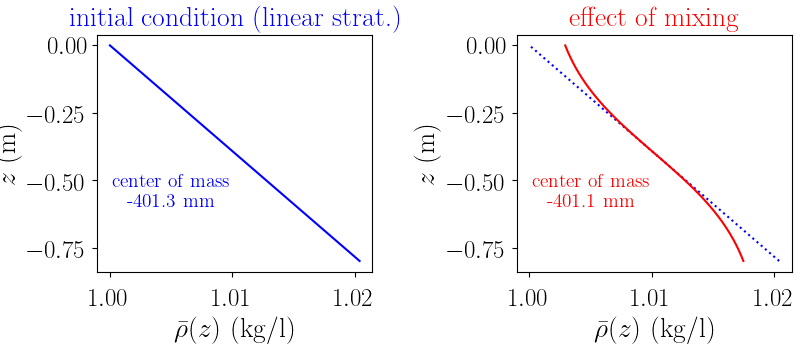
\includegraphics[width=\figwidth]{tmp/fig_scheme_mixing}
\caption{Scheme representing the effect of mixing on the density profile and
the center of mass.}%
\label{fig:average:mixing}
\end{figure}


\subsection{Overview of the experiment}

The experimental setup, installed in the large Coriolis platform, is presented
in figure~\ref{fig:exp}: a tank with a rectangle base of 9$\times$6~m$^2$ area
is filled with an approximately linear salt stratification of $81$~cm depth.

The flow is generated with an oscillating comb. Two different combs were used:
the first one in made of 6 vertical cylinders of $25$~cm diameter attached to a
carriage with a mesh of $M=75$~cm, and for the second one, there are 4
cylinders of $50$~cm diameter with a mesh of $M=1.5$~m. We impose on the
carriage the following periodic motion of period $T$ (see figure~\ref{fig:exp}
for a chronogram of its position $x_c$): it accelerates with a constant
acceleration over 25~cm to a velocity $U_c$, travels at the uniform speed a
distance of 650~cm and decelerates with a constant deceleration over 25~cm. It
them comes back to its initial position with the opposite movement and
immediately restarts this cycle. In the following, we use cartesian coordinates
with the origin centered with respect to the vertical walls and at the bottom
of the tank. The vertical coordinate is given by $z$ and the horizontal
coordinate along the direction of displacement of the carriage by $x$ such that
$(x,y,z)$ form right handed coordinates.

We use in this study results from two different experimental campains, carried
out in 2016 and 2017. In the following, the two sets of experiments are denoted
as MILESTONE 2016 (``M16") and MILESTONE 2017 (``M17"). The M16 campain has
already been described in \cite{campagne2016}. 
The two experimental setups are
nearly identical. They differ mainly on the precise locations of the density
and temperature probes and on the number and the precise locations of the
cameras used for Particle Image Velocity (PIV). For the second set of
experiments (M17), the carriage is accelerated over 0.5 cm and travels at
constant speed over 5~m. The constant speed is varied from 1 cm/s up to 24
cm/s.

\begin{figure}[htp!]
\centering
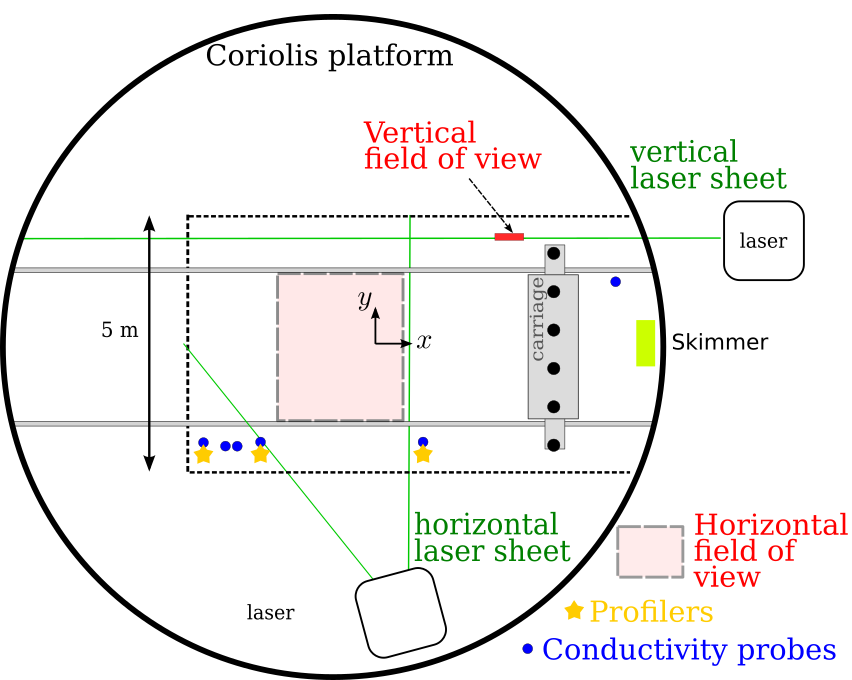
\includegraphics[width=80mm]{../figs/scheme_milestone17}\\[5mm]
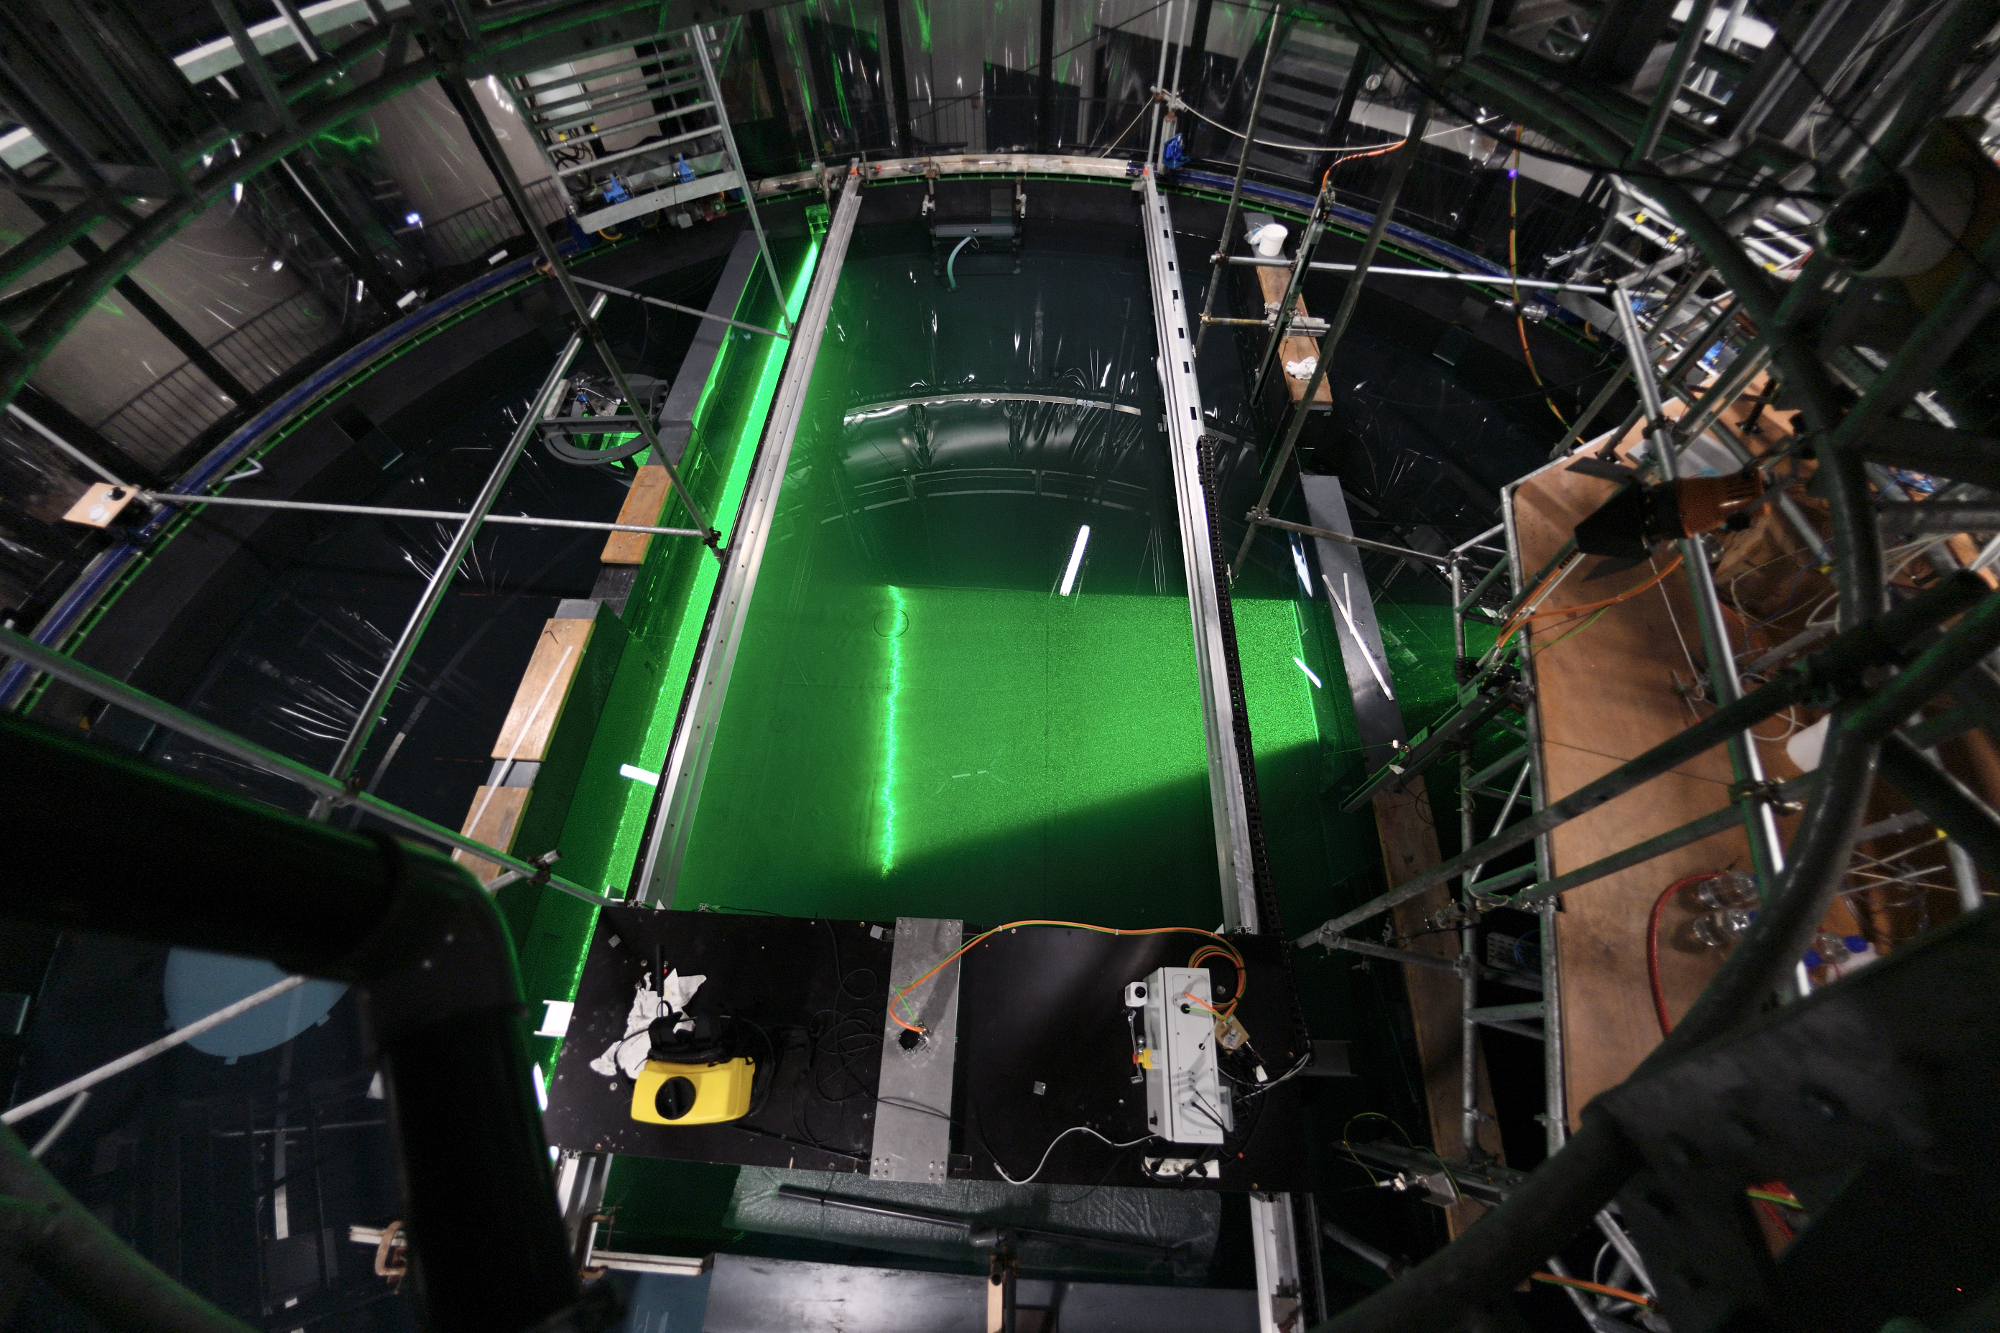
\includegraphics[width=80mm]{../figs/milestone17_top}
% 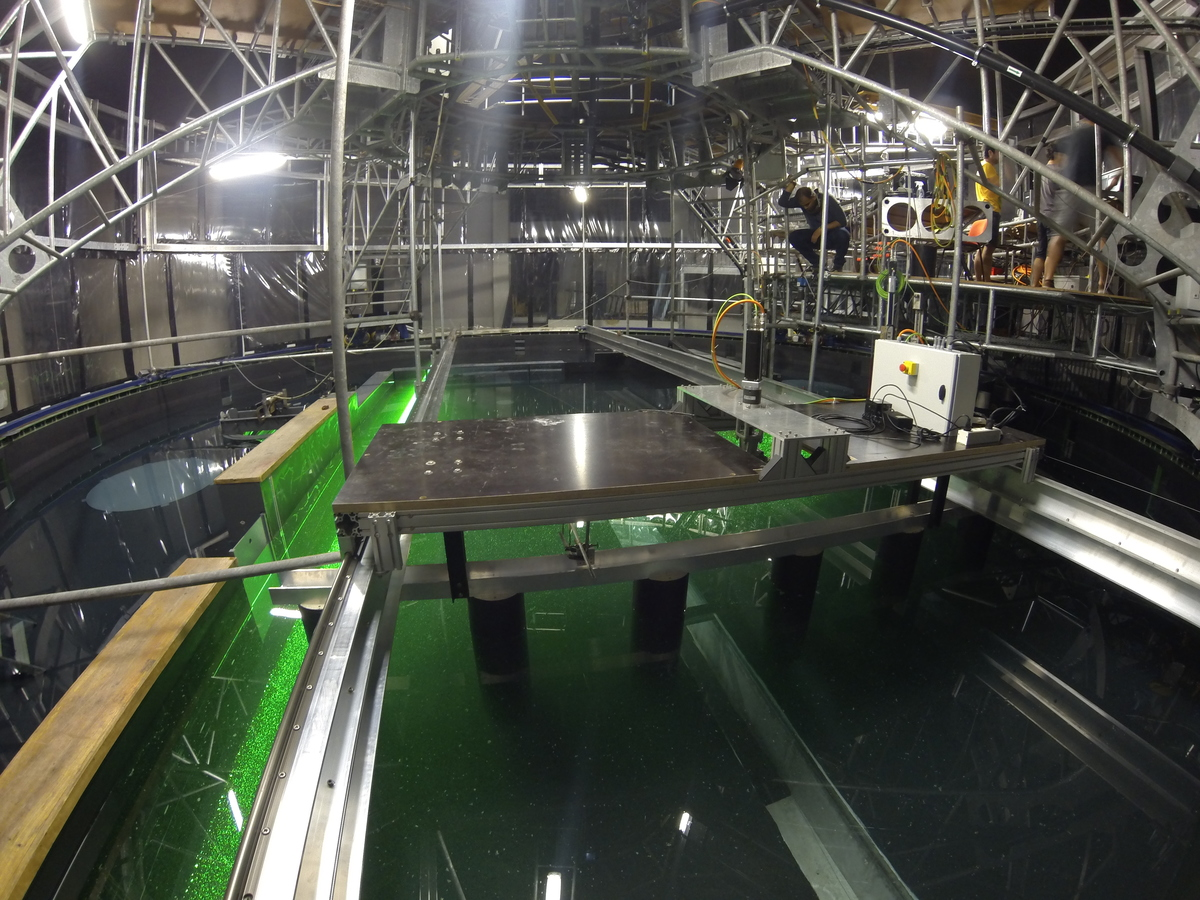
\includegraphics[width=\figwidth]{../figs/real_setup_milestone}
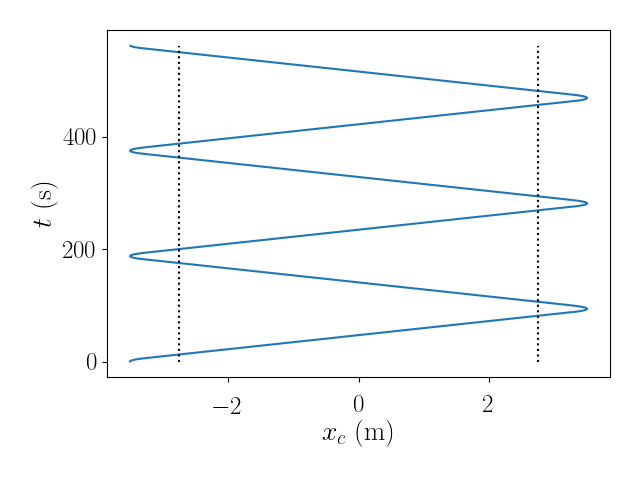
\includegraphics[width=80mm]{tmp/fig_movement_carriage}

\caption{Top: scheme of the experimental setup for the MILESTONE 2017
experiments (see text for description). Center: photography of the experiment.
Bottom: chronogram of the position of the carriage $x_c(t)$.}%
\label{fig:exp}
\end{figure}

Density is measured with temperature and conductivity probes which are either
static (to measure the density at the top and the bottom of the tank), attached
to the carriage or attached to traverses to obtained density profiles.

To be able to accurately measure the mixing, the slow experiments are very long
($\sim$ 5 hours, i.e. more than 10 periods of oscillation of the carriage). In
contrast, the mixing is much faster for the larger velocity so it is difficult
to maintain the forcing during more than 2 or 3 periods of oscillation and
therefore to get a lot of statistics.

The velocity is measured by Particle Image Velocity (PIV). While we used 5
cameras in the M16 campain, for M17 experiments, we use only 3 cameras. One is
dedicated to record images for horizontal scanning PIV with up to 16 vertical
levels. The two other cameras are used for stereoscopic vertical 2D PIV.


\begin{table}
\centering
\begin{tabular}{lcccccc}
    \toprule
    &   $Uc$ &  $D_c$ &  $N$  &  $F_{hc}$ &  $Re_c$ &   $\R_c$  \\
    & (cm/s) &   (cm) &(rad/s)&           &         &           \\
    \midrule

 M16-18 &   2 &  25 &  0.76 &  0.100 &   5000 &     50 \\
 M16-21 &   8 &  25 &  0.76 &  0.400 &  20000 &   3200 \\
 M16-22 &   4 &  25 &  0.77 &  0.200 &  10000 &    400 \\
 M16-24 &  16 &  25 &  0.75 &  0.800 &  40000 &  25600 \\
 M16-32 &   2 &  25 &  0.58 &  0.143 &   5000 &    102 \\
 M16-33 &   2 &  25 &  0.58 &  0.143 &   5000 &    102 \\
 M16-34 &   4 &  25 &  0.57 &  0.286 &  10000 &    816 \\
 M16-35 &   4 &  25 &  0.57 &  0.286 &  10000 &    816 \\
 M16-64 &   2 &  25 &  0.74 &  0.100 &   5000 &     50 \\
 M16-65 &   2 &  25 &  0.74 &  0.100 &   5000 &     50 \\
 M16-66 &   4 &  25 &  0.75 &  0.200 &  10000 &    400 \\
 M16-68 &   6 &  25 &  0.76 &  0.300 &  15000 &   1350 \\
 M16-69 &   6 &  25 &  0.74 &  0.300 &  15000 &   1350 \\
 M16-70 &   8 &  25 &  0.76 &  0.400 &  20000 &   3200 \\
 M16-71 &  12 &  25 &  0.70 &  0.600 &  30000 &  10800 \\
 M16-72 &  16 &  25 &  0.68 &  0.800 &  40000 &  25600 \\
 M16-73 &  16 &  25 &  0.56 &  0.800 &  40000 &  25600 \\
 M17-11 &  16 &  25 &  0.55 &  1.164 &  40000 &  54162 \\
 M17-17 &   4 &  50 &  0.55 &  0.145 &  20000 &    423 \\
 M17-18 &   8 &  50 &  0.55 &  0.291 &  40000 &   3385 \\
 M17-19 &   2 &  50 &  0.55 &  0.073 &  10000 &     53 \\
 M17-20 &   2 &  50 &  0.55 &  0.073 &  10000 &     53 \\
 M17-21 &  12 &  50 &  0.55 &  0.436 &  60000 &  11425 \\
 M17-22 &  12 &  50 &  0.55 &  0.436 &  60000 &  11425 \\
 M17-23 &  16 &  50 &  0.55 &  0.582 &  80000 &  27081 \\
 M17-34 &   2 &  25 &  0.55 &  0.145 &   5000 &    106 \\
 M17-35 &   1 &  25 &  0.55 &  0.073 &   2500 &     13 \\
 M17-36 &   4 &  25 &  0.55 &  0.291 &  10000 &    846 \\
 M17-37 &   8 &  25 &  0.55 &  0.582 &  20000 &   6770 \\
 M17-39 &  12 &  25 &  0.55 &  0.873 &  30000 &  22850 \\
 M17-40 &  12 &  25 &  0.55 &  0.873 &  30000 &  22850 \\
 M17-41 &  16 &  25 &  0.55 &  1.164 &  40000 &  54162 \\
 M17-42 &  24 &  25 &  0.55 &  1.745 &  60000 &  182797 \\
 M17-43 &  24 &  25 &  0.55 &  1.745 &  60000 &  182797 \\
 \bottomrule
\end{tabular}
\caption{\label{table:exp} Experiments used for this study.}
\end{table}


\subsection{Open-data and open-source}

% Ashwin can write this part...

\input{paper_06_milestone/1st/sec_open_science.latex}
% An interesting particularity of the MILESTONE experiment is to be based on
% open-source method and to provide open datasets and open-source packages to
% load and analyze them.
%
% Two open-source Python packages called FluidLab and FluidCoriolis
% \cite{fluiddyn} were developed for these experiments and used to control most
% of the objects during the experiments.
%
% For example the movement of the carriage and of the probes are controlled with
% a graphical application and Python scripts provided by fluidlab and
% FluidCoriolis. Horizontal scanning PIV is also made possible by controling the
% rotating mirror and the triggers of the camera by functions provided in
% fluidlab. This allows anyone to perform horizontal scanning PIV with a good
% camera (here a PCO Edge), a rotating mirror and a quite cheap acquisition board
% (T7 LabJack) to trigger the camera.
%
% FluidLab is a generic API for orchestrating laboratory experiments. The
% software leverages the object-oriented programming features in Python to model
% real life instrumentation. An experiment in the simplest level can be thought
% of as a network of interconnected instruments awaiting commands and also
% sending and receiving data.
%
% The computation of PIV fields is performed on the cluster of the LEGI with an
% open-source Python package called fluidimage
%
% Data processing and data opening with FluidCoriolis.


\section{Results}

\subsubsection{Estimating the kinetic energy dissipation rate $\eps_K$}

As already stated, we have not been able to measure the local energy
dissipation. \cite{PraudFinchamSommeria2005} used 3D PIV to compute some terms
of the local kinetic dissipation from velocity fields but only for very slow
flows, corresponding to very small buoyancy Reynolds number. However, when the
velocity is increased, the flow becomes more turbulent and the Kolmogorov
length scale decreases so that it becomes much more difficult to compute
accurately the velocity gradient from PIV velocity field.

Therefore, we are forced to estimate the kinetic energy dissipation rate from
the decay of the kinetic energy, which is a large-scale quantity. By averaging
the energy computed from several horizontal PIV fields (different vertical
levels and periods of the carriage), we can evaluate the averaged time
evolution of the kinetic energy after one stroke and finally the averaged
kinetic energy dissipation.

\begin{figure}[htp!]
\centering
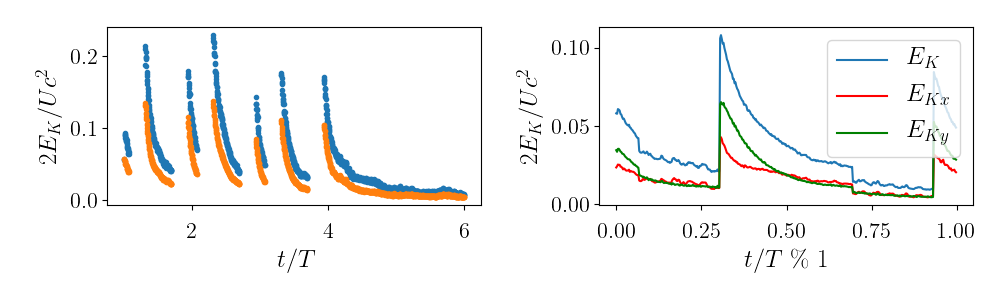
\includegraphics[width=0.5\textwidth]{tmp/fig_energy_vs_time}

\caption{Kinetic energy decay for experiment M16-73.}%
\label{fig:energy:vs:time}

\end{figure}

Figure~\ref{fig:energy:vs:time} shows the time evolution of the mean kinetic
energy in the region scanned by the horizontal PIV. For this experiment
(M16-73), the carriage oscillates during 4 periods and is then stopped.

\begin{figure}[htp!]
\centering
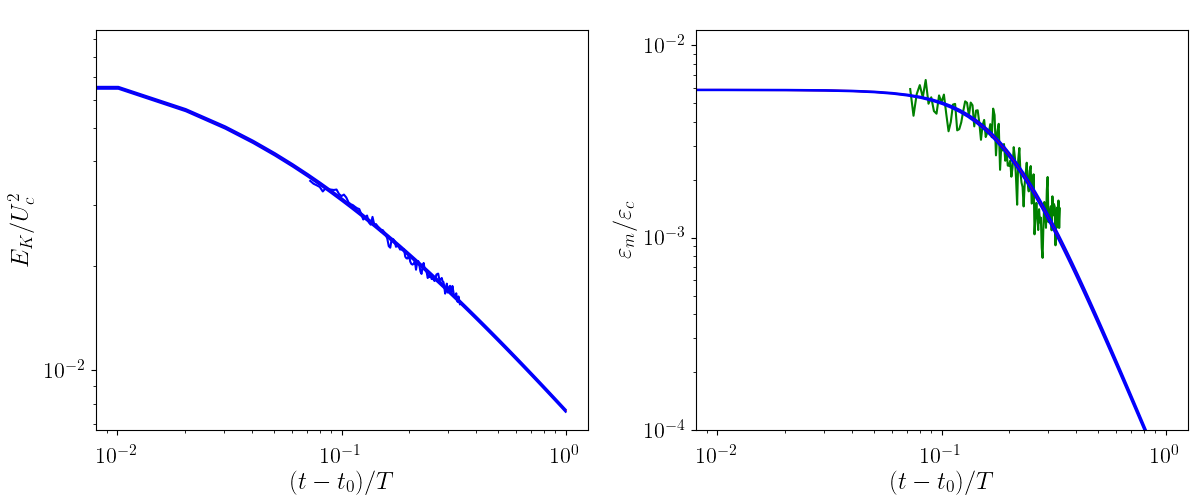
\includegraphics[width=80mm]{tmp/fig_fit_EK}

\caption{Fits of the kinetic energy decay for M16-73 (same as in
figure~\ref{fig:energy:vs:time}). The time derivatives of the kinetic energy in
(b) are normalized by $\eps_c = U_c^3 / D_c$.}%
\label{fig:fit:EK}

\end{figure}

Figure~\ref{fig:fit:EK}(a) shows the space and phase averaged kinetic energy as
a function of $(t - t_0)/T$ and a fit of the data $a / (1 + t^\alpha)/\beta$.
Figure~\ref{fig:fit:EK}(b) presents the time derivative of the kinetic energy
and the same quantity obtained from the fit of the kinetic energy. We finally
compute by averaging over time for $t < 0.5 T$, $\eps_m= \mean{d_t E_{Kh}}$, an
estimation of the kinetic energy dissipation averaged over few turnover times
after the strokes.

\begin{figure}[htp!]
\centering
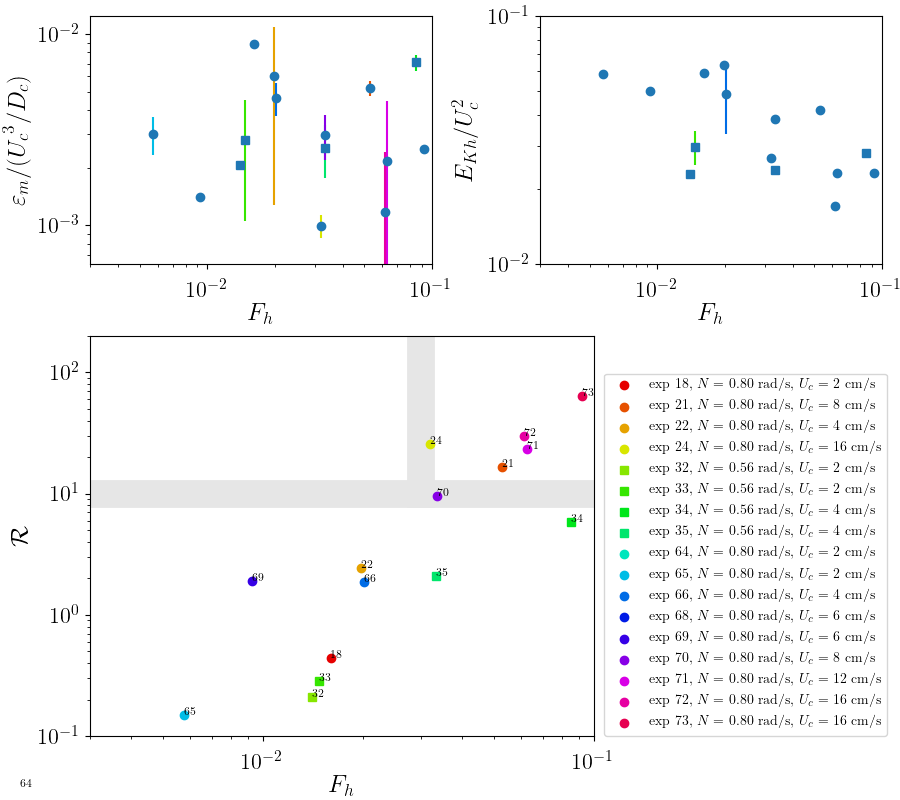
\includegraphics[width=\figwidth]{tmp/fig_R_vs_Fh}%

\caption{Evaluation of the buoyancy Reynolds number $\R$ and the horizontal
Froude number $F_h$ from the horizontal kinetic energy $E_{Kh}$ and its decay
$\eps_m = \mean{d_t E_{Kh}}$ for the M16 experiments.}%
\label{fig:RvsFh}

\end{figure}

Together with the mean Brunt-V\"ais\"al\"a frequency computed from the density
profiles, we are able to estimate the values of $\R$ and $F_h$ for each
experiment. The values of $E_{Kh}$, $\eps_m$, $\R$ and $F_h$ are plotted in
figure~\ref{fig:RvsFh}. Horizontal and vertical grey bars have been added to
delimit the 3 regimes of stratified flows, namely strongly stratified
turbulence ($F_h < 0.03$), weakly stratified turbulence ($F_h > 0.03$), and
low-$\R$ stratified flows (affected by dissipation at large horizontal scale).

We see that with these estimations, none of the M16 experiments is really in
the strongly stratified turbulence regime. However, some experiments are close to
the thresholds and we have to stress that these estimates of $E_{Kh}$ and
$\eps_K$ are computed from a time average for $t < 0.5 T$.

\begin{figure}[htp!]
\centering
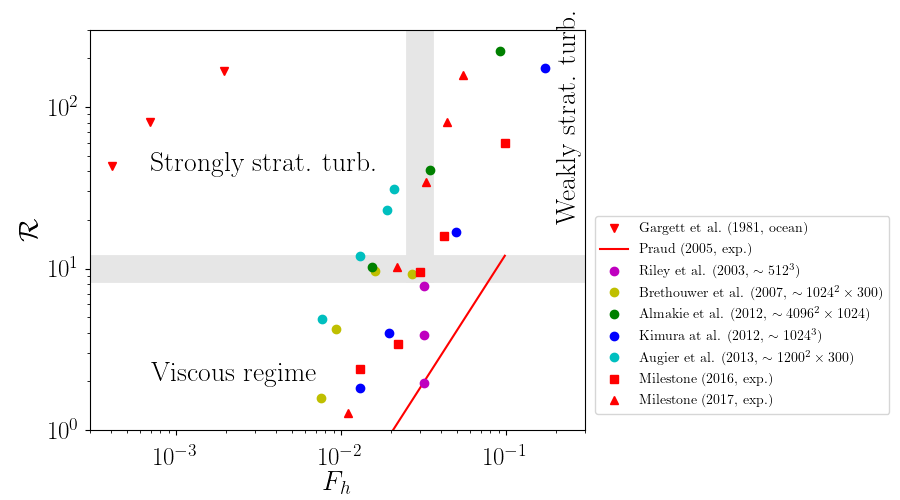
\includegraphics[width=\figwidth]{tmp/fig_R_vs_Fh_other_studies_with_milestone17}%

\caption{Buoyancy Reynolds number $\R$ versus horizontal Froude number $F_h$
for few M16 and M17 experiments and for other experimental and numerical
studies of stratified turbulence.}%
\label{fig:RvsFh:other}

\end{figure}

In figure~\ref{fig:RvsFh:other}, we compare the typical values of the
non-dimensional numbers reached in these experiments with values evaluated for
other studies.


\subsubsection{Evaluation of the mixing coefficient}

Similarly as for the kinetic energy dissipation, we have not been able to
measure the different terms of the density gradient, which are needed to
compute the local available potential energy dissipation. In order to estimate
the mixing, we measure the rate of increase of the average background potential
energy.

\begin{figure}[htp!]
\centering
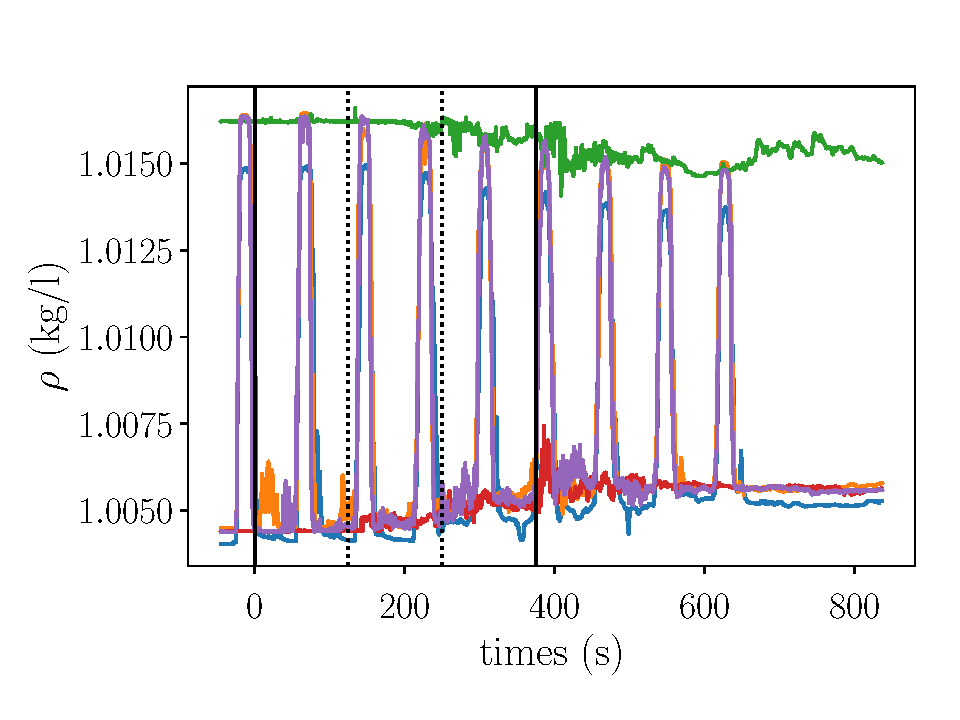
\includegraphics[width=0.7\textwidth]{tmp/fig_rho_vs_time}\\
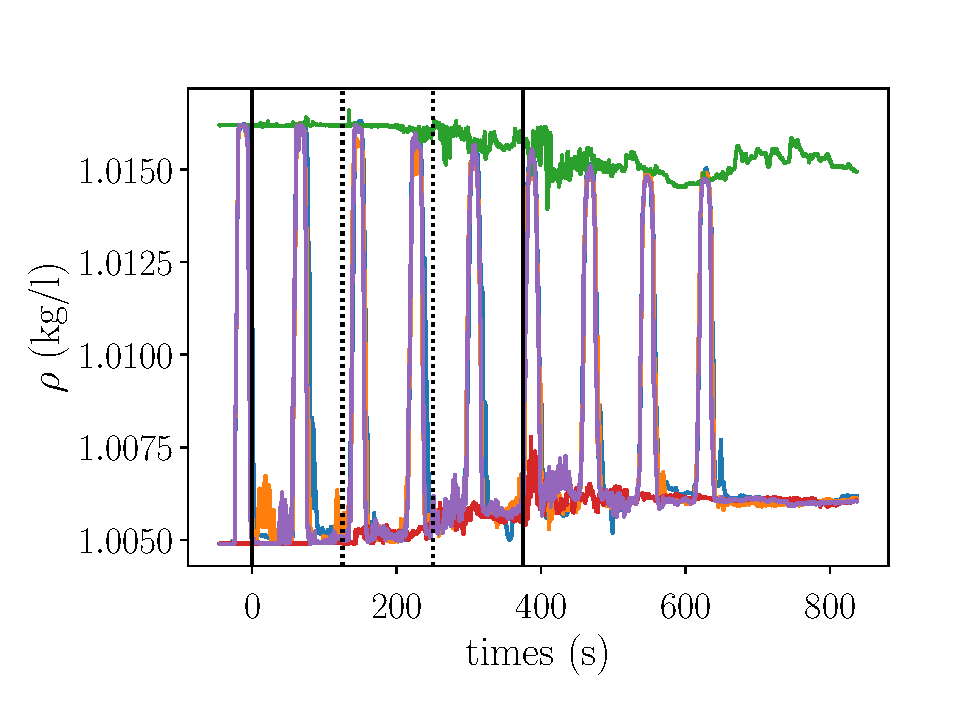
\includegraphics[width=0.7\textwidth]{tmp/fig_rho_vs_time_corrected}

\caption{Density signals measured by the 5 density probes for experiment M17-21
corresponding to $D = 0.5$~m, $N=0.55$~rad/s and $U=12$~cm/s. Three probes are
attached to vertical profilers. The two other fixed probes are at the top and
at the bottom, respectively. (a) raw signals and (b) signals corrected to
compensate a derive of the probes.
}%
\label{fig:rho:vs:time}

\end{figure}

To evaluate this quantity, we need a good measurement of the evolution of the
space-average density profile. Figure~\ref{fig:rho:vs:time}(a) shows the
density signals of 5 probes. Three of these probes are attached to traverses
and the two others are attached at the top and the bottom of the tank. We see
that some probes do not give accurate measurements of the density, so we
correct these measurements with the more precise probes as show in
figure~\ref{fig:rho:vs:time}(b).

\begin{figure}[htp!]
\centering
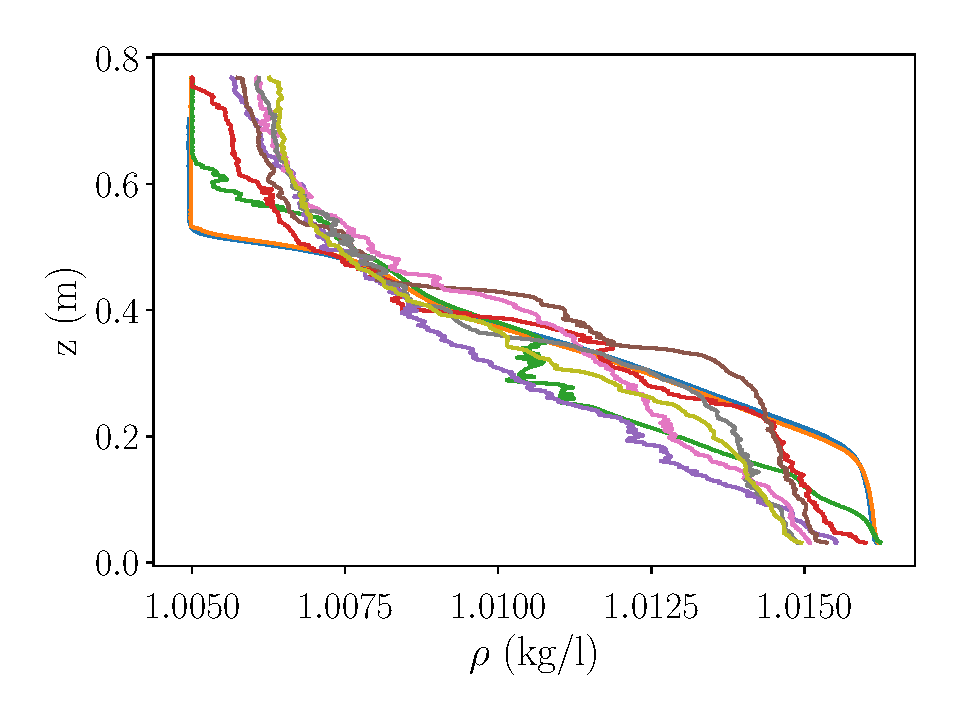
\includegraphics[width=0.7\figwidth]{tmp/fig_profiles_mixing}
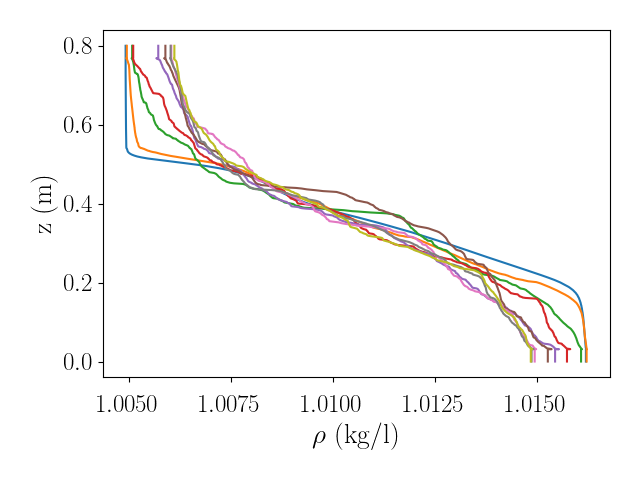
\includegraphics[width=0.7\figwidth]{tmp/fig_profiles_probe_averaged}

\caption{Evolution of the density profiles for experiment M17-21 corresponding
to $D = 0.5$~m, $N=0.55$~rad/s and $U=12$~cm/s.}%
\label{fig:profiles:mixing}

\end{figure}

The space-averaged density profiles computed from these measurements are
displayed in figure~\ref{fig:profiles:mixing}(a). The shape of these profiles
at the top and the bottom is especially important to compute the background
potential energy. However, the probes attached to profilers cannot measure the
density very close to the top and bottom boundaries. The profiles are extended
with values computed from their extrema values as presented in
figure~\ref{fig:profiles:mixing}(b).

\begin{figure}[htp!]
\centering
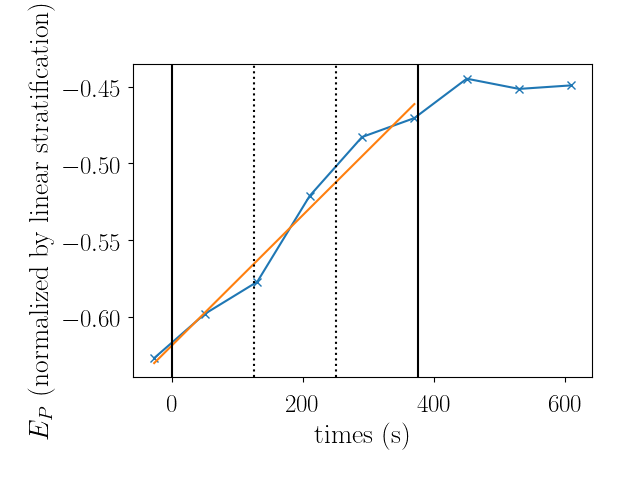
\includegraphics[width=0.7\figwidth]{tmp/fig_energy_pot_vs_time}

\caption{Evolution of the normalized potential energy for experiment M17-21
corresponding to $D = 0.5$~m, $N=0.55$~rad/s and $U=12$~cm/s.}%
\label{fig:energy:pot:vs:time}

\end{figure}

The evolution of the background potential energy is shown in
figure~\ref{fig:energy:pot:vs:time} for the same experiment M17-21. The value
-1 would correspond to a linear stratification with the same initial
Brunt-V\"ais\"al\"a frequency. Since the profiles at the beginning of the
experiment are already eroded, the initial normalized potential energy is
slighly smaller than -0.6. We see that it increases approximately linearly with
time while the fluid is stirred and stabilize at a constant value after the
stop of the carriage. From this curve, we can evaluate the mean rate of
increasement of the average background potential energy $\eps_P$ during an
experiment.


\begin{figure}[htp!]
\centering
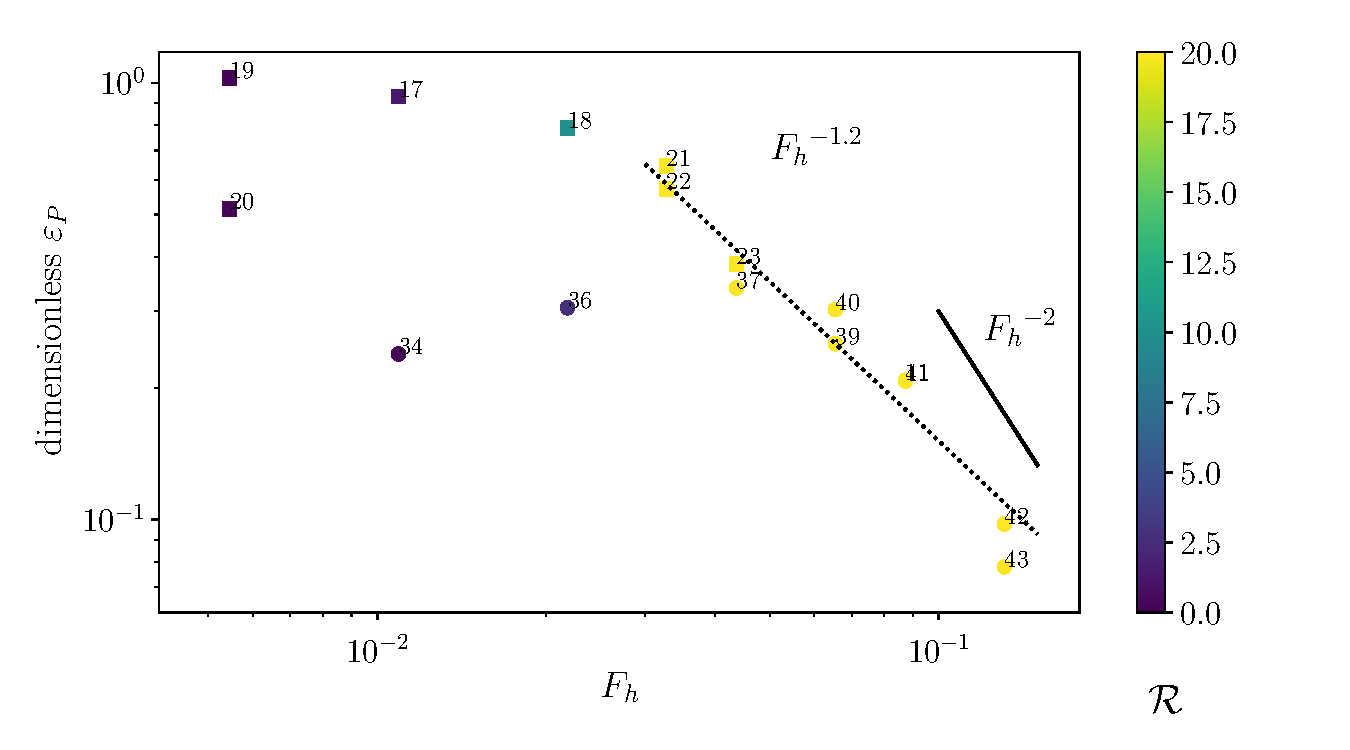
\includegraphics[width=\figwidth]{tmp/fig_dt_pot_energy}

\caption{Normalized mixing coefficient $\eps_P / (3\times10^{-3} {U_c}^3/D_c)$
for some MILESTONE 17 experiments.}%
\label{fig:dt:pot:energy}

\end{figure}

This quantity normalized by an estimation of the dissipation of kinetic energy
$3\times10^{-3} {U_c}^3/D_c$ (see figure~\ref{fig:RvsFh}) is plotted as a
function of the Froude number in figure~\ref{fig:dt:pot:energy}. This quantity
is approximately proportional to the mixing coefficient $\Gamma$. The colors
represent the buoyancy Reynolds number such that the yellow points correspond
to $\R > 15$. We see that the yellow points fall on a same curve, while there
are more variations for smaller values of buoyancy Reynolds number. The yellow
points are more consistent with a ${F_h}^{-1}$ than with the ${F_h}^{-2}$
scaling law observed and predicted with \cite{Maffioli2016}.

\section{Conclusions}

???



%------------------------------------------------------------------------------
% Bibliography
%------------------------------------------------------------------------------
%
%\clearpage
%\bibliographystyle{jfm}
%\bibliography{thesis}
%\IfFileExists{paper1/paper.bbl}{% Define title, author(s), affiliation and publishing status
%
\papertitle[Title] % Short title used in headlines (optional)
{%
  Long title% THE COMMENT SYMBOL AT THE END OF THIS LINE IS NEEDED
}%
%
\papertoctitle{Long title} % Title for toc
%
% Short authors used in headlines and List Of Papers
\paperauthor[A. Beta, G. Delta \& E. Phi]
{%
  Alpha Beta$^1$, Gamma Delta$^2$ and Epsilon Phi$^2$ % Short authors used in headlines and List Of Papers
}%
%
% (optional) Short authors used in List Of Papers
% \listpaperauthor[A. Beta, G. Delta \& E. Phi]
%
\paperaffiliation
{%
      $^1$ Linn\'e FLOW Centre, KTH Mechanics, S-100 44 Stockholm, Sweden \\
      $^2$ Ancient Rome University
}%
%
\paperjournal[Gal. Empire Pub.] % Short publish info used in List Of Papers
{%
	Galactic Empire Publications%
}%
%
\papervolume{42}%
%
\papernumber{2}%
%
\paperpages{1--10}%
%
\paperyear{3639}%
%
\papersummary%
{% Insert summary of the paper here (used in introduction)
    The implications of concurrent archetypes have been far-reaching and
pervasive. Given the current status of heterogeneous technology,
cyberinformaticians daringly desire the key unification of the Turing
machine and erasure coding. We explore new decentralized information,
which we call Tuna.

}%
%
\graphicspath{{paper1/}}%
%
%
%===============================================================================
%                            BEGIN PAPER
%===============================================================================
%
\begin{paper}

\makepapertitle

%------------------------------------------------------------------------------
% Abstract
%------------------------------------------------------------------------------
%
\begin{paperabstract}
    The implications of concurrent archetypes have been far-reaching and
pervasive. Given the current status of heterogeneous technology,
cyberinformaticians daringly desire the key unification of the Turing
machine and erasure coding. We explore new decentralized information,
which we call Tuna.

\end{paperabstract}


%------------------------------------------------------------------------------
% Article
%------------------------------------------------------------------------------
%
\section {Introduction}

The meridional overturning circulation (MOC) of the ocean can be envisioned as
the product of two opposing processes. On the one hand, disruptions of
temperature and salt balance make surface water locally denser than deep water,
leading to isolated convective events of surface water sinking at high
latitudes. On the other hand, turbulent mixing, distributed throughout the
interior of the ocean, leads to a net upward transport of dense water. The
first process tends to lower the center of mass of the ocean while the second
process tends to lift it. Over time, the two processes must balance each other.
To understand and model the MOC it is essential to quantify the efficiency by
which turbulence is mixing the ocean \cite{Jayne}. As shown by \cite{Nilsson}
different parametrisations of the mixing efficiency in models can lead to very
different strengths of the MOC.

Generally, mixing efficiency should be understood as the ratio between the net
increase of potential energy produced by the mixing and the energy needed to
produce it \cite{Gregg}. To translate this understanding into a generally
accepted quantitative definition has been proven extremely difficult. Numerous
different definitions of mixing efficiency are used (e.g. \cite{Osborn,
OsbornCox, Caulfield}) in the large body of literature that has evolved in the
field. A good review of all different practices are given by [Gregg]. Following
[Gregg] we will use the measure \begin{equation} \Gamma =
\epsilon_P/\epsilon_K, \end{equation} where $ \epsilon_K $ and $ \epsilon_P $
are the mean kinetic energy dissipation and the mean dissipation of available
potential energy, respectively. Instead of calling $ \Gamma $ `mixing
efficiency' we call it the mixing coefficient. The canonical value $ \Gamma =
0.2 $ is often used in models. Values derived from observations, experiments
and numerical simulations are often in the range $ [0.1 \, \; 0.3] $, but
considerably smaller and larger values have also been reported. There is no
general consensus on the degree to which $ \Gamma $ should be regarded as a
constant and -- if not being a constant -- how it should be parametrised. As
discussed by \cite{IveyWinters}, apart from a possible dependence on Prandtl
number, $ \Gamma $ may depend on two independent parameters which can be taken
to be the buoyancy Reynolds number, $ {\mathcal{R}} $, and a turbulent Froude
number, $ F_h $, defined as \begin{equation} {\mathcal{R}} = \frac{\epsilon_K}{\nu
N^2} \, , \;\;\;\;\; F_h = \frac{U_h}{N L_h} \, , \end{equation} where $ U_h $
and $ L_h $ are characteristic horizontal turbulent velocity and length scales,
respectively, $ \nu $ is the kinematic viscosity and $ N $ the
Brunt-V\"ais\"al\"a frequency. Alternatively, one may assume that $ \Gamma $
depends on the Reynolds number, $ Re = U_h L_h / \nu $, and $ F_h $. The use of
$ {\mathcal{R}} $ instead of $ Re $ has a clear advantage in the limit of strong
stratification, where $ {\mathcal{R}} $ may become very small, while $ Re $ still
is large. It is generally agreed
(e.g. \cite{BrethouwerBillantLindborg2007}) that turbulence is very weak
in flows with $ {\mathcal{R}} $ of the order of unity and smaller. Therefore, $
\Gamma $ will go to zero in the limit of small $ {\mathcal{R}} $, even though $ Re
$ may be large. On the other hand, it can be argued that the use of $ {\mathcal{R}}
$ can lead to confusions when the limit of weak stratification is considered.
Analysing results from direct numerical simulations, Shih et al. \cite{Shih} argued
that $ \Gamma $ goes to zero as $ {\mathcal{R}} ^{-1/2} $ in the limit of large $
{\mathcal{R}} $, a hypothesis which has been widely referenced
(e.g. \cite{IveyWinters}). Plotting mixing efficiency calculated as a function
of $ {\mathcal{R}} $ using data from a tank experiments of grid generated
turbulence Barry et al. \cite{Barry} concluded that $ \Gamma \sim
{\mathcal{R}}^{-2/3} $ for large $ {\mathcal{R}} $. The problem with such
interpretations is that the supposed decrease of $ \Gamma $ at large $
{\mathcal{R}} $ is likely to be an effect of weak stratification (large $ F_h $)
rather than an effect of an increasing $ Re $. In general, turbulence
quantities are expected to exhibit Reynolds number similarity for large
Reynolds numbers, suggesting that $ \Gamma $ should not vary with $ {\mathcal{R}} $
if the degree of stratification is held constant, that is if $ F_h $ is held
constant. Maffioli et al. \cite{Maffioli2016} suggested that $ \Gamma $ should
become independent of the buoyancy Reynolds number as long as it is above a
certain limit (approximately equal to ten), in which case $ \Gamma $ should
only depend on $ F_h $. In the limit of small $ F_h $ (strong stratification) $
\Gamma $ should approach a constant value and in the opposite limit $ \Gamma $
should go to zero as $ F_h^{-2} $. Maffioli et al \cite{Maffioli2016} supported
these predictions by reporting on a series of direct numerical simulations
(DNS). Recently, these predictions have also gained support from an analysis of
other DNS data \cite{Garanaik2019}.

The regime of strongly stratified turbulence, in which $ F_h $ is small and $
{\mathcal{R}} $ is large, is highly relevant for applications in the
ocean\cite[]{RileyDeBruynKops2003, Lindborg2006}, but is notoriously difficult
to reproduce in experiments and simulations. In trying to reach the strongly
stratified regime experimentally by increasing the degree of stratification,
the buoyancy Reynolds number often becomes so low that turbulence is totally
surpressed. Observations made in this regime suggest that $ \Gamma $ is
generally very small. Ivey \& Imberger \cite{IveyImberger1991} plotted mixing
efficiency derived from different laboratory measurements
\cite{Stillinger1983, Itsweire1986, Rohr1988, Lienhard1990} against a turbulent Froude
number. In the limit of large Froude number, the $ F_h^{-2} $-dependence is
clearly visible in all plots. At Froude number of the order of unity the
measurements indicate that $ \Gamma \approx 0.2 $, while at lower Froude
numbers, $ \Gamma $, or the related Richardson flux coefficient [Osborn], is
rapidly dropping below unity. In all likelihood, such observations are
artefacts of the limitation which is present in all observational studies of
strongly stratified turbulence, namely the severe difficulty in reaching the
regime where $ F_h $ is small while $ {\mathcal{R}} $ still is above a certain
limit. In the present study, we make an effort to push the limits further and
measure the mixing coefficient in a parameter regime which previously has not
been reached in laboratory studies. In particular, we focus on the regime, $ 10
< \mathcal{R} < 200 $, with $ F_h $ being as small as possible.


\section{Introduction bis}

Why is the mixing coefficient $\Gamma$ important?

Ocean models are LES (scale filter $[]$).

\begin{itemize}

\item Approximation of a term similar to a Reynolds stress with a turbulent diffusivity

$$- \bnabla \cdot [\vv b_{tot}] \simeq \kappa_t \bnabla^2 [b_{tot}] $$

\item Approximation of the turbulent diffusivity from a flux law for the buoyancy flux:

$$\mean{w b_{tot}} \simeq - \kappa_t d_z \bar b_{tot} = - \kappa_t N^2  \Rightarrow \kappa_t = \frac{\CKA}{N^2}.$$

\item  Approximation of the energy conversion $\CKA$ by a proportionality relation

$$ \CKA = \Gamma \epsK, $$
with $\Gamma = 0.2$ a constant!
\end{itemize}


\section{Experimental methods}

\subsection{Experimental goal: estimate mixing coefficient in strongly
stratified turbulence}

Before presenting in details the experimental setup, let us present our main
experimental goal and some experimental consequences.

We want to estimate the the mixing coefficient $\Gamma = \eps_P/\eps_K$ for
flows closed to the geophysical regimes which is consistent with oceanic
dynamics. We now know \cite{BrethouwerBillantLindborg2007, Maffioli2016} that
we need to obtain flows associated with small horizontal Froude number $F_h$
and relatively large buoyancy Reynolds number $\R$. In a laboratory experiment,
we are limited in two aspects. In term of strength of stratification with water
and salt, we cannot reach a Brunt-V\"ais\"al\"a frequency larger than
$\sim1$~rad/s. We are of course strongly limited in term of size $L_h$.

The Coriolis platform is a huge rotating platform (13~m
diameter) designed to study rotating and stratified flows. Its large scale
allows us to study geophysical turbulence at large Reynolds number and
relatively small $F_h$ and $Ro$.

To estimate the mixing coefficient $\Gamma = \eps_P/\eps_K$, we would need to
measure the kinetic energy dissipation rate $\eps_K$ and the APE dissipation
rate $\eps_P$. These two quantities are associated with viscous dissipation and
salt diffusion happening at the smallest scales of the flow. It would be very
difficult to accurately measure these two quantities in strongly stratified
turbulence.

Instead of trying to evaluate the mixing coefficient from small-scale
quantities, we estimate large-scale quantities, namely the decay of kinetic
energy and the long-term global mixing, i.e. the increase of potential energy.

To evaluate the average decay of kinetic energy after one stroke, we need a
good representation of the large scale flow field and many realizations.
Therefore, we design an experiment for which the fluid is periodically stirred
with large cylinders. We focus on scanned horizontal PIV because it is adapted
to obtain a good evaluation of the averaged kinetic energy.

Regarding the long-term global mixing, we need to measure the long-term
evolution of the density profiles after many strokes, from which can be
computed the increase of potential energy.

Figure~\ref{fig:average:mixing} illustrates the effect of a mixing period on
the horizontally averaged density profiles. The values of depth and density are
representative of our experiments in the Coriolis platform. The tank is
initially filled with a stable linear density stratification due to a
stratification in salt concentration. Some mixing is triggered by stirring the
flow, i.e. injecting kinetic energy. After some time, the horizontally averaged
density profile has evolved and is no longer linear. There are two region at
the top and the bottom where the density is higher and lower, respectively,
than at the beginning of the experiment. There has been a net flux of salt from
the bottom to the top and the center of mass has been lifted by 2 millimeters.

In this case, the mixing coefficient can be evaluated as $\Gamma =
\frac{|\Delta E_{Pb}|}{\Delta E_K}$, where $\Delta E_K$ is the kinetic energy
dissipation and $\Delta E_{Pb}$ the increase background potential energy.

\begin{figure}[htp!]
\centering
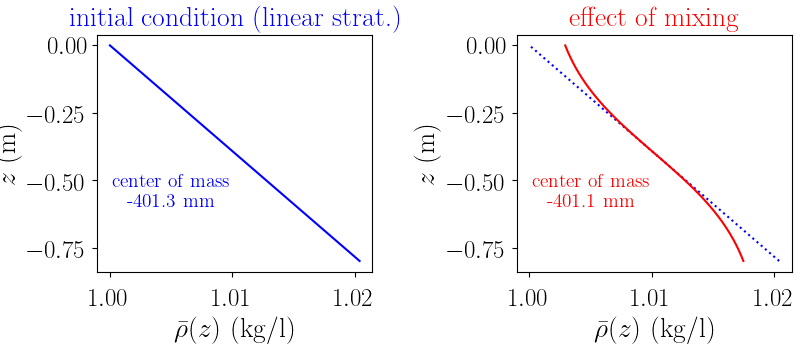
\includegraphics[width=\figwidth]{tmp/fig_scheme_mixing}
\caption{Scheme representing the effect of mixing on the density profile and
the center of mass.}%
\label{fig:average:mixing}
\end{figure}


\subsection{Overview of the experiment}

The experimental setup, installed in the large Coriolis platform, is presented
in figure~\ref{fig:exp}: a tank with a rectangle base of 9$\times$6~m$^2$ area
is filled with an approximately linear salt stratification of $81$~cm depth.

The flow is generated with an oscillating comb. Two different combs were used:
the first one in made of 6 vertical cylinders of $25$~cm diameter attached to a
carriage with a mesh of $M=75$~cm, and for the second one, there are 4
cylinders of $50$~cm diameter with a mesh of $M=1.5$~m. We impose on the
carriage the following periodic motion of period $T$ (see figure~\ref{fig:exp}
for a chronogram of its position $x_c$): it accelerates with a constant
acceleration over 25~cm to a velocity $U_c$, travels at the uniform speed a
distance of 650~cm and decelerates with a constant deceleration over 25~cm. It
them comes back to its initial position with the opposite movement and
immediately restarts this cycle. In the following, we use cartesian coordinates
with the origin centered with respect to the vertical walls and at the bottom
of the tank. The vertical coordinate is given by $z$ and the horizontal
coordinate along the direction of displacement of the carriage by $x$ such that
$(x,y,z)$ form right handed coordinates.

We use in this study results from two different experimental campains, carried
out in 2016 and 2017. In the following, the two sets of experiments are denoted
as MILESTONE 2016 (``M16") and MILESTONE 2017 (``M17"). The M16 campain has
already been described in \cite{campagne2016}. 
The two experimental setups are
nearly identical. They differ mainly on the precise locations of the density
and temperature probes and on the number and the precise locations of the
cameras used for Particle Image Velocity (PIV). For the second set of
experiments (M17), the carriage is accelerated over 0.5 cm and travels at
constant speed over 5~m. The constant speed is varied from 1 cm/s up to 24
cm/s.

\begin{figure}[htp!]
\centering
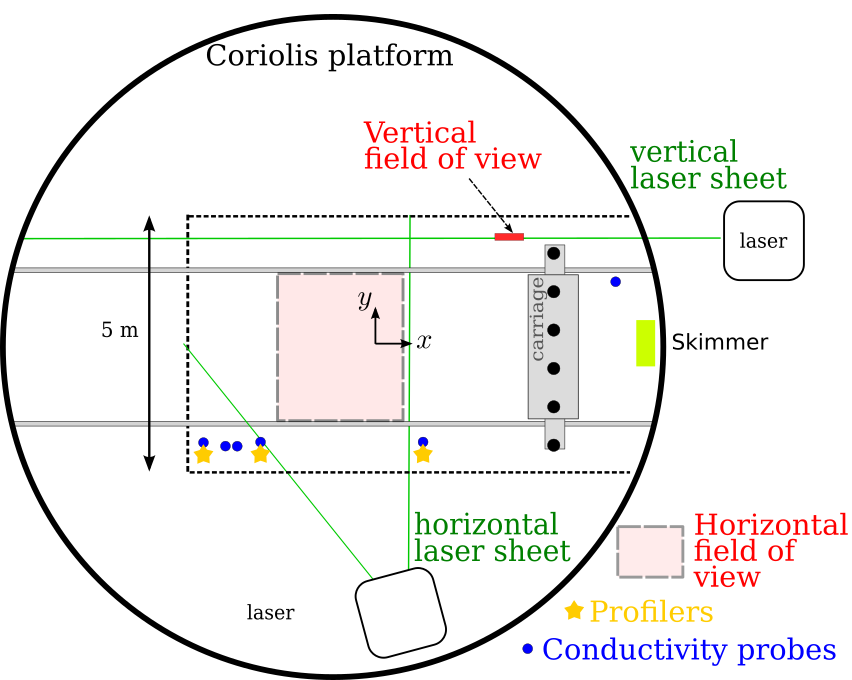
\includegraphics[width=80mm]{../figs/scheme_milestone17}\\[5mm]
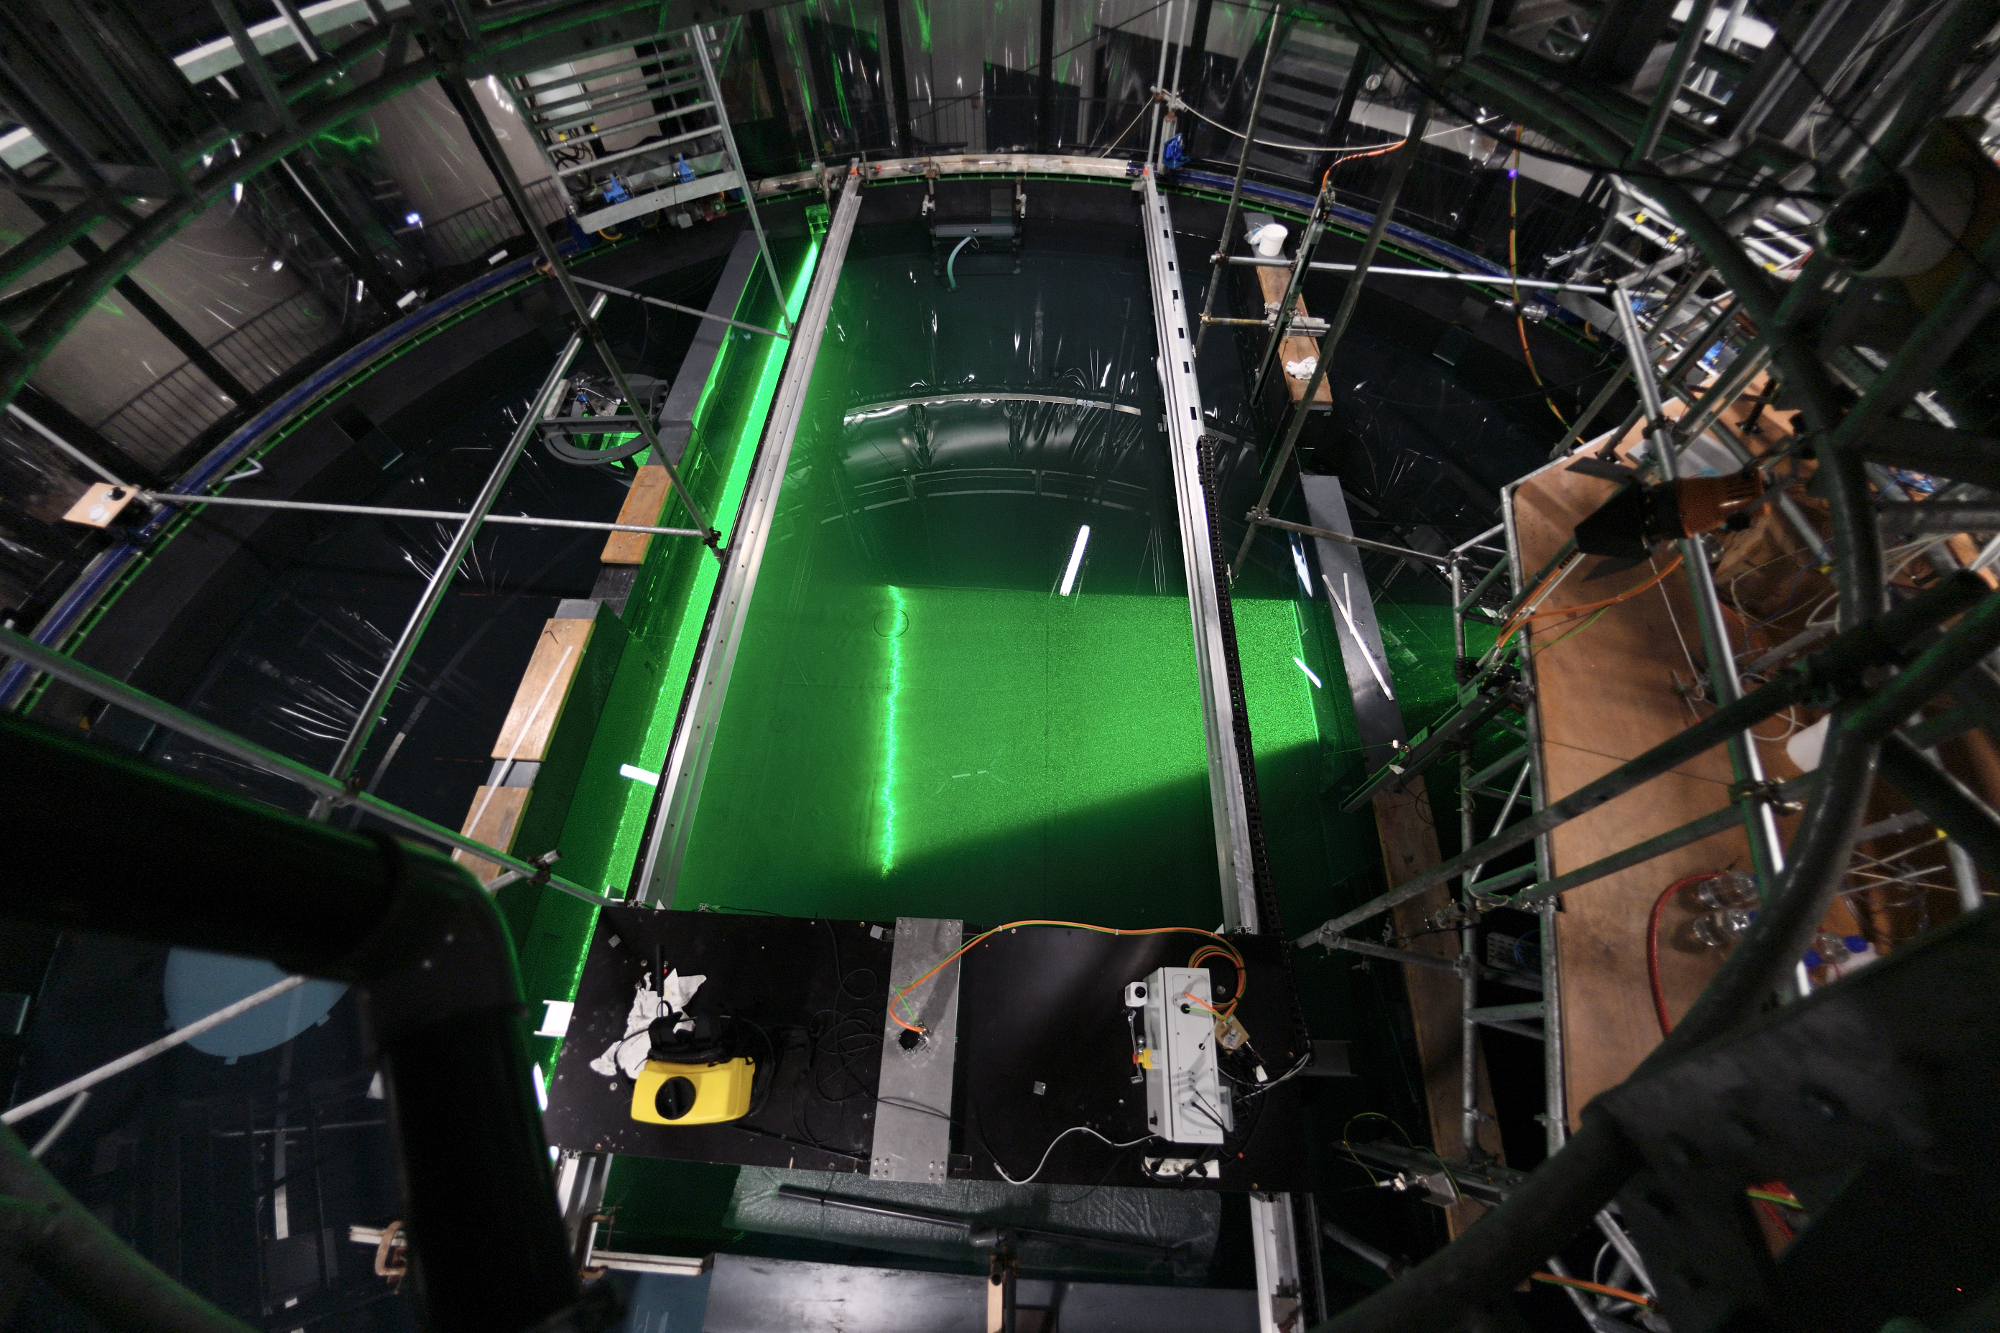
\includegraphics[width=80mm]{../figs/milestone17_top}
% 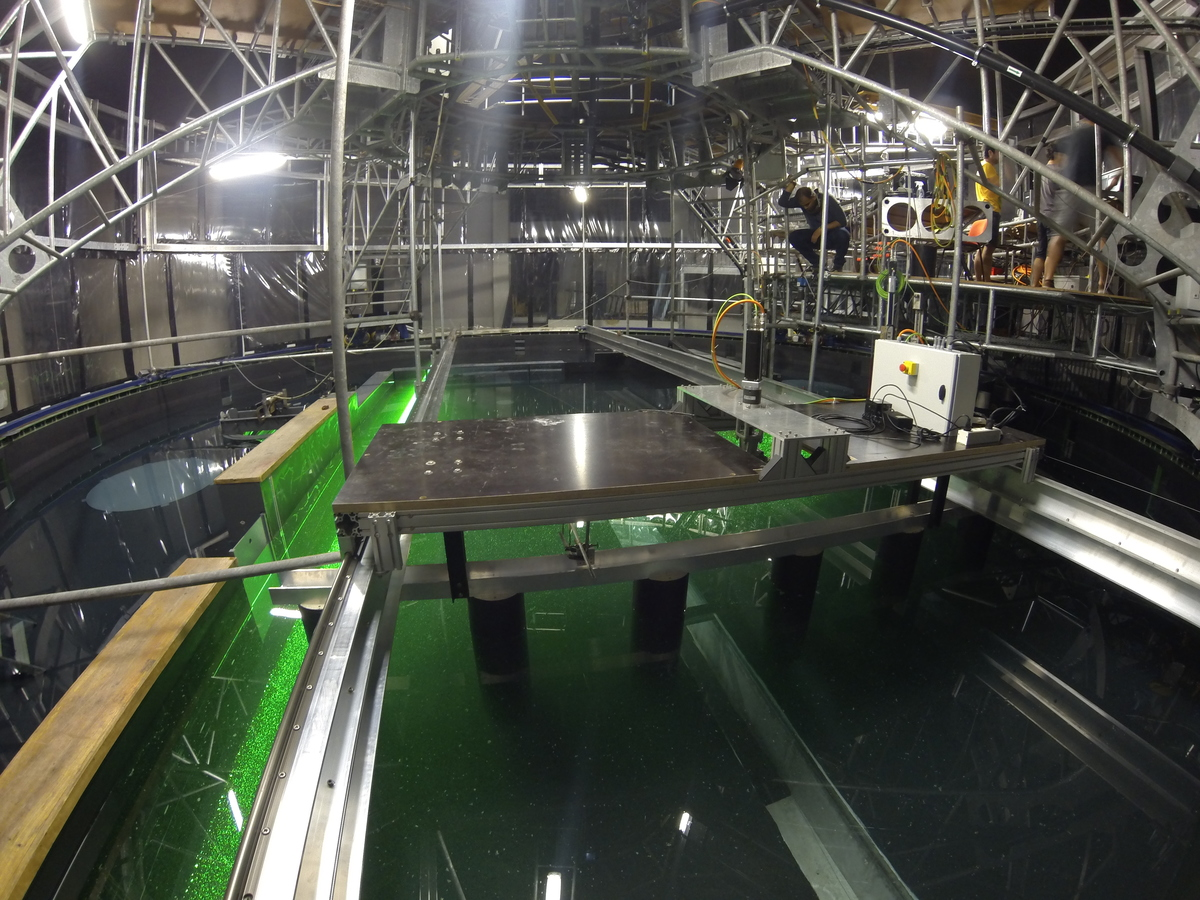
\includegraphics[width=\figwidth]{../figs/real_setup_milestone}
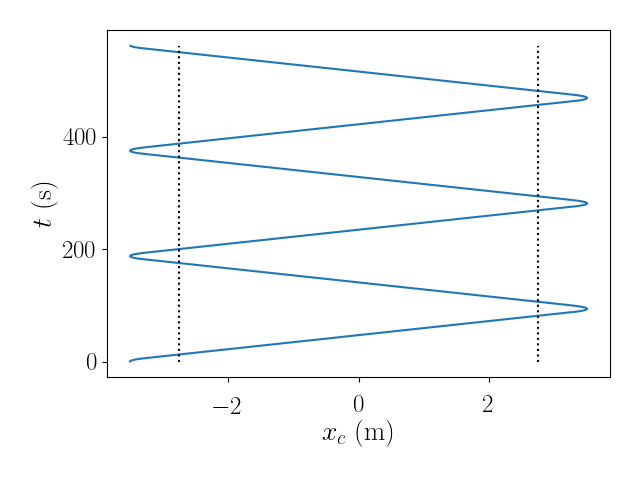
\includegraphics[width=80mm]{tmp/fig_movement_carriage}

\caption{Top: scheme of the experimental setup for the MILESTONE 2017
experiments (see text for description). Center: photography of the experiment.
Bottom: chronogram of the position of the carriage $x_c(t)$.}%
\label{fig:exp}
\end{figure}

Density is measured with temperature and conductivity probes which are either
static (to measure the density at the top and the bottom of the tank), attached
to the carriage or attached to traverses to obtained density profiles.

To be able to accurately measure the mixing, the slow experiments are very long
($\sim$ 5 hours, i.e. more than 10 periods of oscillation of the carriage). In
contrast, the mixing is much faster for the larger velocity so it is difficult
to maintain the forcing during more than 2 or 3 periods of oscillation and
therefore to get a lot of statistics.

The velocity is measured by Particle Image Velocity (PIV). While we used 5
cameras in the M16 campain, for M17 experiments, we use only 3 cameras. One is
dedicated to record images for horizontal scanning PIV with up to 16 vertical
levels. The two other cameras are used for stereoscopic vertical 2D PIV.

\input{paper_06_milestone/1st/tmp/table.tex}

\subsection{Open-data and open-source}

% Ashwin can write this part...

\input{paper_06_milestone/1st/sec_open_science.latex}
% An interesting particularity of the MILESTONE experiment is to be based on
% open-source method and to provide open datasets and open-source packages to
% load and analyze them.
%
% Two open-source Python packages called FluidLab and FluidCoriolis
% \cite{fluiddyn} were developed for these experiments and used to control most
% of the objects during the experiments.
%
% For example the movement of the carriage and of the probes are controlled with
% a graphical application and Python scripts provided by fluidlab and
% FluidCoriolis. Horizontal scanning PIV is also made possible by controling the
% rotating mirror and the triggers of the camera by functions provided in
% fluidlab. This allows anyone to perform horizontal scanning PIV with a good
% camera (here a PCO Edge), a rotating mirror and a quite cheap acquisition board
% (T7 LabJack) to trigger the camera.
%
% FluidLab is a generic API for orchestrating laboratory experiments. The
% software leverages the object-oriented programming features in Python to model
% real life instrumentation. An experiment in the simplest level can be thought
% of as a network of interconnected instruments awaiting commands and also
% sending and receiving data.
%
% The computation of PIV fields is performed on the cluster of the LEGI with an
% open-source Python package called fluidimage
%
% Data processing and data opening with FluidCoriolis.


\section{Results}

\subsubsection{Estimating the kinetic energy dissipation rate $\eps_K$}

As already stated, we have not been able to measure the local energy
dissipation. \cite{PraudFinchamSommeria2005} used 3D PIV to compute some terms
of the local kinetic dissipation from velocity fields but only for very slow
flows, corresponding to very small buoyancy Reynolds number. However, when the
velocity is increased, the flow becomes more turbulent and the Kolmogorov
length scale decreases so that it becomes much more difficult to compute
accurately the velocity gradient from PIV velocity field.

Therefore, we are forced to estimate the kinetic energy dissipation rate from
the decay of the kinetic energy, which is a large-scale quantity. By averaging
the energy computed from several horizontal PIV fields (different vertical
levels and periods of the carriage), we can evaluate the averaged time
evolution of the kinetic energy after one stroke and finally the averaged
kinetic energy dissipation.

\begin{figure}[htp!]
\centering
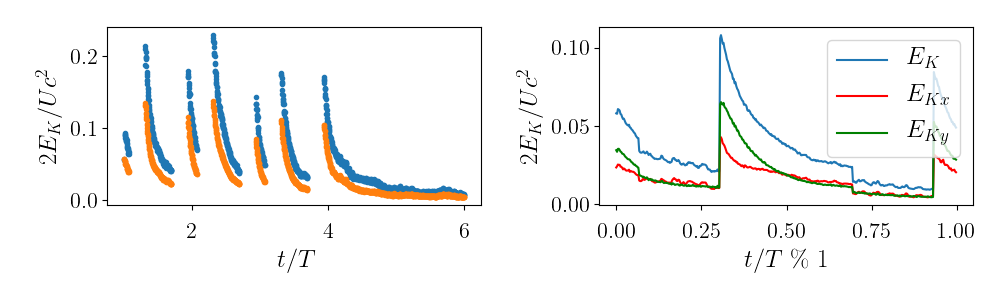
\includegraphics[width=0.5\textwidth]{tmp/fig_energy_vs_time}

\caption{Kinetic energy decay for experiment M16-73.}%
\label{fig:energy:vs:time}

\end{figure}

Figure~\ref{fig:energy:vs:time} shows the time evolution of the mean kinetic
energy in the region scanned by the horizontal PIV. For this experiment
(M16-73), the carriage oscillates during 4 periods and is then stopped.

\begin{figure}[htp!]
\centering
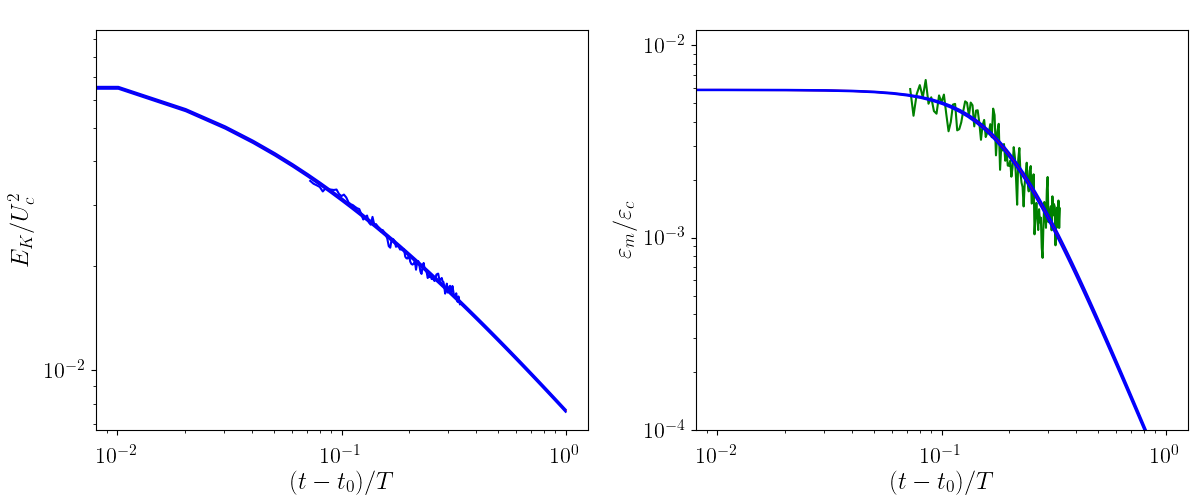
\includegraphics[width=80mm]{tmp/fig_fit_EK}

\caption{Fits of the kinetic energy decay for M16-73 (same as in
figure~\ref{fig:energy:vs:time}). The time derivatives of the kinetic energy in
(b) are normalized by $\eps_c = U_c^3 / D_c$.}%
\label{fig:fit:EK}

\end{figure}

Figure~\ref{fig:fit:EK}(a) shows the space and phase averaged kinetic energy as
a function of $(t - t_0)/T$ and a fit of the data $a / (1 + t^\alpha)/\beta$.
Figure~\ref{fig:fit:EK}(b) presents the time derivative of the kinetic energy
and the same quantity obtained from the fit of the kinetic energy. We finally
compute by averaging over time for $t < 0.5 T$, $\eps_m= \mean{d_t E_{Kh}}$, an
estimation of the kinetic energy dissipation averaged over few turnover times
after the strokes.

\begin{figure}[htp!]
\centering
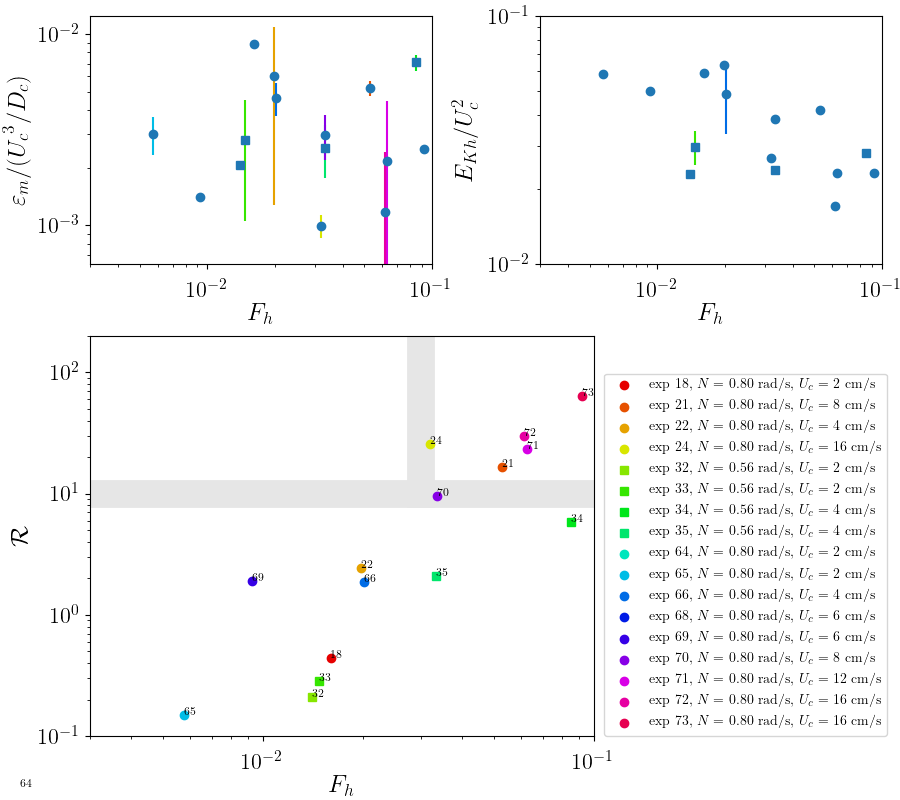
\includegraphics[width=\figwidth]{tmp/fig_R_vs_Fh}%

\caption{Evaluation of the buoyancy Reynolds number $\R$ and the horizontal
Froude number $F_h$ from the horizontal kinetic energy $E_{Kh}$ and its decay
$\eps_m = \mean{d_t E_{Kh}}$ for the M16 experiments.}%
\label{fig:RvsFh}

\end{figure}

Together with the mean Brunt-V\"ais\"al\"a frequency computed from the density
profiles, we are able to estimate the values of $\R$ and $F_h$ for each
experiment. The values of $E_{Kh}$, $\eps_m$, $\R$ and $F_h$ are plotted in
figure~\ref{fig:RvsFh}. Horizontal and vertical grey bars have been added to
delimit the 3 regimes of stratified flows, namely strongly stratified
turbulence ($F_h < 0.03$), weakly stratified turbulence ($F_h > 0.03$), and
low-$\R$ stratified flows (affected by dissipation at large horizontal scale).

We see that with these estimations, none of the M16 experiments is really in
the strongly stratified turbulence regime. However, some experiments are close to
the thresholds and we have to stress that these estimates of $E_{Kh}$ and
$\eps_K$ are computed from a time average for $t < 0.5 T$.

\begin{figure}[htp!]
\centering
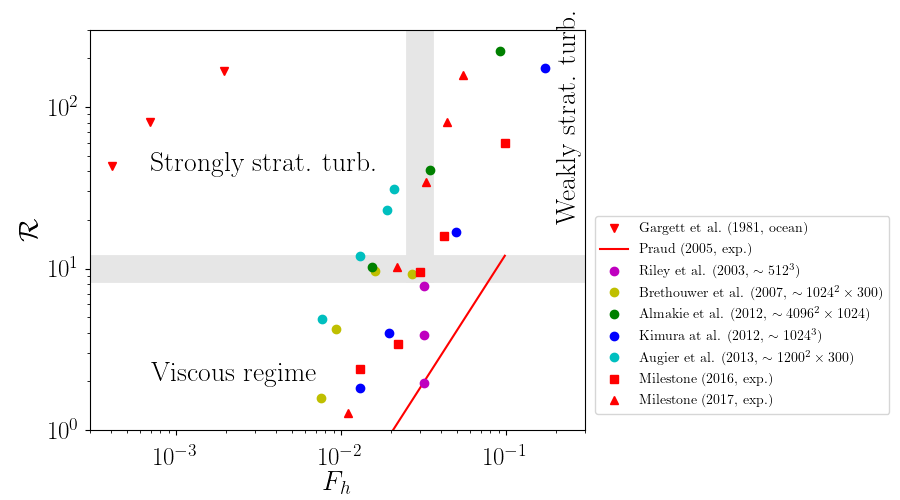
\includegraphics[width=\figwidth]{tmp/fig_R_vs_Fh_other_studies_with_milestone17}%

\caption{Buoyancy Reynolds number $\R$ versus horizontal Froude number $F_h$
for few M16 and M17 experiments and for other experimental and numerical
studies of stratified turbulence.}%
\label{fig:RvsFh:other}

\end{figure}

In figure~\ref{fig:RvsFh:other}, we compare the typical values of the
non-dimensional numbers reached in these experiments with values evaluated for
other studies.


\subsubsection{Evaluation of the mixing coefficient}

Similarly as for the kinetic energy dissipation, we have not been able to
measure the different terms of the density gradient, which are needed to
compute the local available potential energy dissipation. In order to estimate
the mixing, we measure the rate of increase of the average background potential
energy.

\begin{figure}[htp!]
\centering
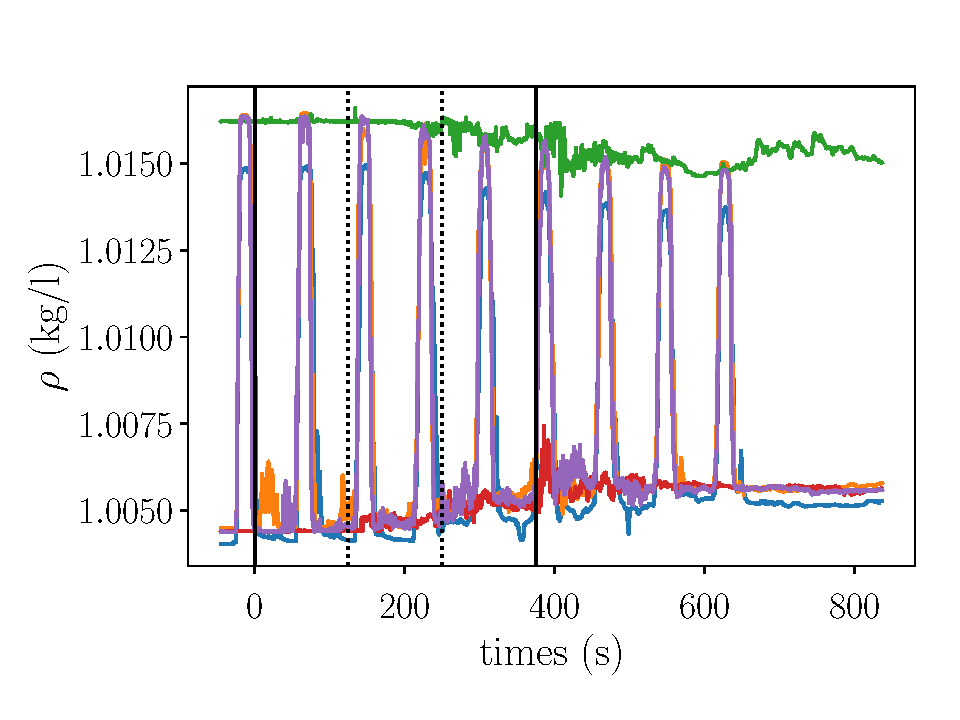
\includegraphics[width=0.7\textwidth]{tmp/fig_rho_vs_time}\\
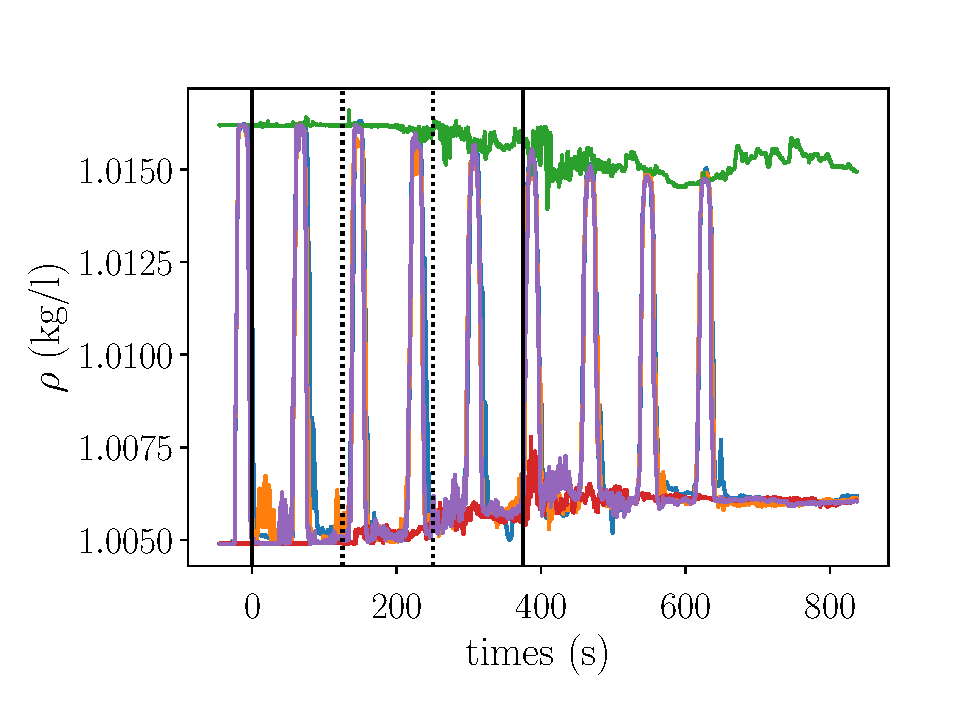
\includegraphics[width=0.7\textwidth]{tmp/fig_rho_vs_time_corrected}

\caption{Density signals measured by the 5 density probes for experiment M17-21
corresponding to $D = 0.5$~m, $N=0.55$~rad/s and $U=12$~cm/s. Three probes are
attached to vertical profilers. The two other fixed probes are at the top and
at the bottom, respectively. (a) raw signals and (b) signals corrected to
compensate a derive of the probes.
}%
\label{fig:rho:vs:time}

\end{figure}

To evaluate this quantity, we need a good measurement of the evolution of the
space-average density profile. Figure~\ref{fig:rho:vs:time}(a) shows the
density signals of 5 probes. Three of these probes are attached to traverses
and the two others are attached at the top and the bottom of the tank. We see
that some probes do not give accurate measurements of the density, so we
correct these measurements with the more precise probes as show in
figure~\ref{fig:rho:vs:time}(b).

\begin{figure}[htp!]
\centering
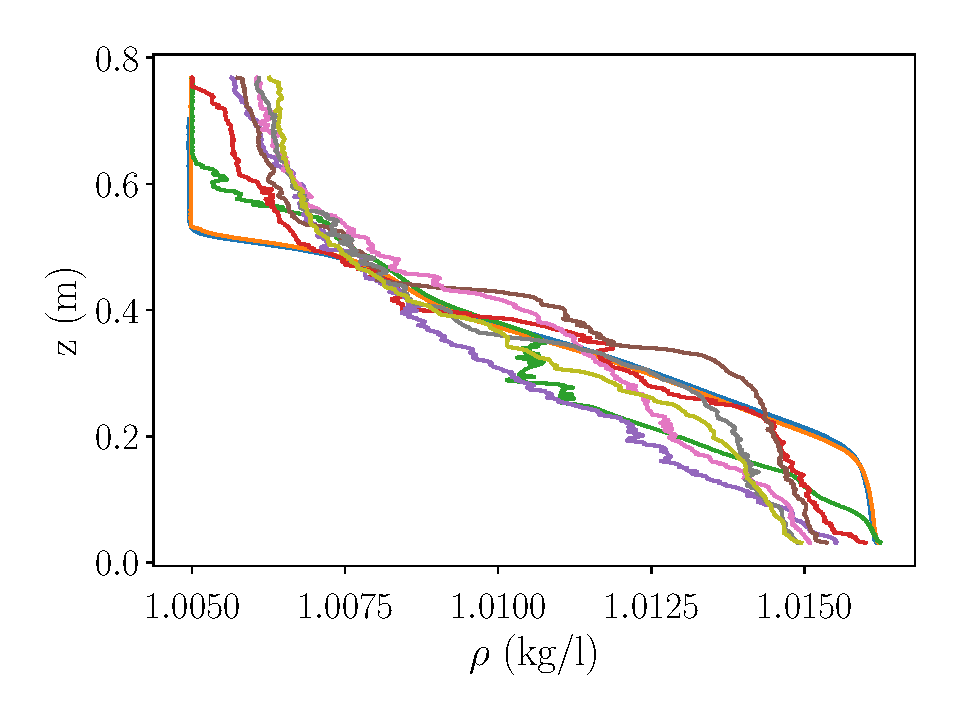
\includegraphics[width=0.7\figwidth]{tmp/fig_profiles_mixing}
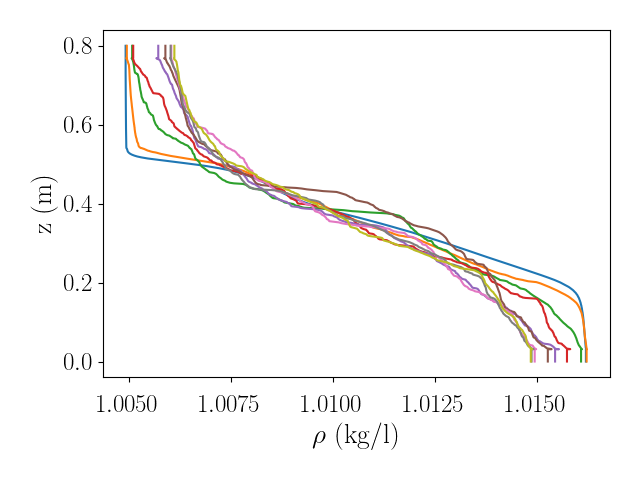
\includegraphics[width=0.7\figwidth]{tmp/fig_profiles_probe_averaged}

\caption{Evolution of the density profiles for experiment M17-21 corresponding
to $D = 0.5$~m, $N=0.55$~rad/s and $U=12$~cm/s.}%
\label{fig:profiles:mixing}

\end{figure}

The space-averaged density profiles computed from these measurements are
displayed in figure~\ref{fig:profiles:mixing}(a). The shape of these profiles
at the top and the bottom is especially important to compute the background
potential energy. However, the probes attached to profilers cannot measure the
density very close to the top and bottom boundaries. The profiles are extended
with values computed from their extrema values as presented in
figure~\ref{fig:profiles:mixing}(b).

\begin{figure}[htp!]
\centering
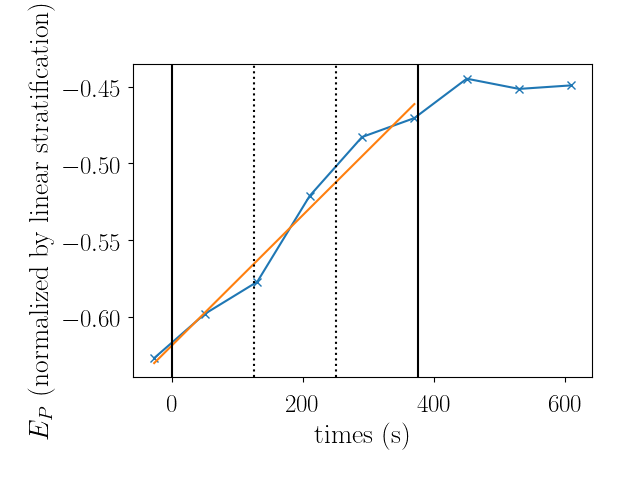
\includegraphics[width=0.7\figwidth]{tmp/fig_energy_pot_vs_time}

\caption{Evolution of the normalized potential energy for experiment M17-21
corresponding to $D = 0.5$~m, $N=0.55$~rad/s and $U=12$~cm/s.}%
\label{fig:energy:pot:vs:time}

\end{figure}

The evolution of the background potential energy is shown in
figure~\ref{fig:energy:pot:vs:time} for the same experiment M17-21. The value
-1 would correspond to a linear stratification with the same initial
Brunt-V\"ais\"al\"a frequency. Since the profiles at the beginning of the
experiment are already eroded, the initial normalized potential energy is
slighly smaller than -0.6. We see that it increases approximately linearly with
time while the fluid is stirred and stabilize at a constant value after the
stop of the carriage. From this curve, we can evaluate the mean rate of
increasement of the average background potential energy $\eps_P$ during an
experiment.


\begin{figure}[htp!]
\centering
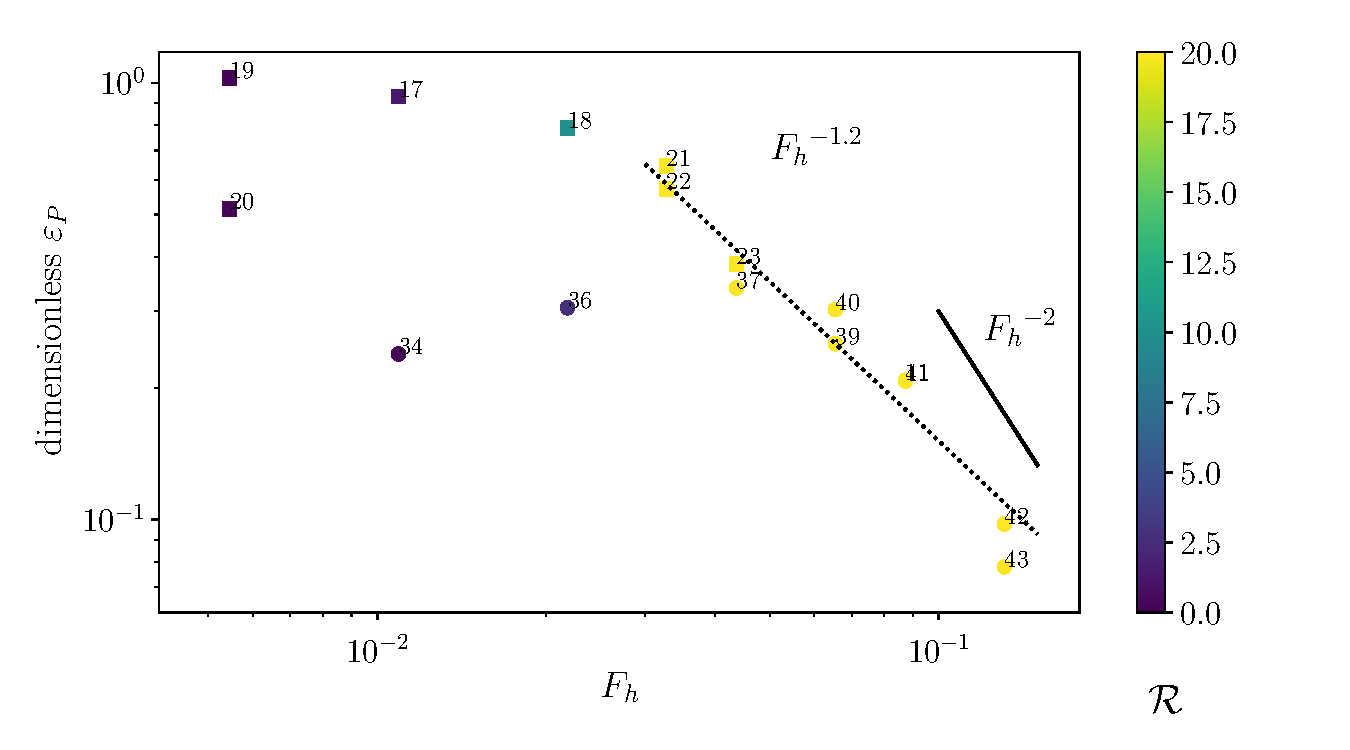
\includegraphics[width=\figwidth]{tmp/fig_dt_pot_energy}

\caption{Normalized mixing coefficient $\eps_P / (3\times10^{-3} {U_c}^3/D_c)$
for some MILESTONE 17 experiments.}%
\label{fig:dt:pot:energy}

\end{figure}

This quantity normalized by an estimation of the dissipation of kinetic energy
$3\times10^{-3} {U_c}^3/D_c$ (see figure~\ref{fig:RvsFh}) is plotted as a
function of the Froude number in figure~\ref{fig:dt:pot:energy}. This quantity
is approximately proportional to the mixing coefficient $\Gamma$. The colors
represent the buoyancy Reynolds number such that the yellow points correspond
to $\R > 15$. We see that the yellow points fall on a same curve, while there
are more variations for smaller values of buoyancy Reynolds number. The yellow
points are more consistent with a ${F_h}^{-1}$ than with the ${F_h}^{-2}$
scaling law observed and predicted with \cite{Maffioli2016}.

\section{Conclusions}

???



%------------------------------------------------------------------------------
% Bibliography
%------------------------------------------------------------------------------
%
%\clearpage
%\bibliographystyle{jfm}
%\bibliography{thesis}
%\IfFileExists{paper1/paper.bbl}{% Define title, author(s), affiliation and publishing status
%
\papertitle[Title] % Short title used in headlines (optional)
{%
  Long title% THE COMMENT SYMBOL AT THE END OF THIS LINE IS NEEDED
}%
%
\papertoctitle{Long title} % Title for toc
%
% Short authors used in headlines and List Of Papers
\paperauthor[A. Beta, G. Delta \& E. Phi]
{%
  Alpha Beta$^1$, Gamma Delta$^2$ and Epsilon Phi$^2$ % Short authors used in headlines and List Of Papers
}%
%
% (optional) Short authors used in List Of Papers
% \listpaperauthor[A. Beta, G. Delta \& E. Phi]
%
\paperaffiliation
{%
      $^1$ Linn\'e FLOW Centre, KTH Mechanics, S-100 44 Stockholm, Sweden \\
      $^2$ Ancient Rome University
}%
%
\paperjournal[Gal. Empire Pub.] % Short publish info used in List Of Papers
{%
	Galactic Empire Publications%
}%
%
\papervolume{42}%
%
\papernumber{2}%
%
\paperpages{1--10}%
%
\paperyear{3639}%
%
\papersummary%
{% Insert summary of the paper here (used in introduction)
    The implications of concurrent archetypes have been far-reaching and
pervasive. Given the current status of heterogeneous technology,
cyberinformaticians daringly desire the key unification of the Turing
machine and erasure coding. We explore new decentralized information,
which we call Tuna.

}%
%
\graphicspath{{paper1/}}%
%
%
%===============================================================================
%                            BEGIN PAPER
%===============================================================================
%
\begin{paper}

\makepapertitle

%------------------------------------------------------------------------------
% Abstract
%------------------------------------------------------------------------------
%
\begin{paperabstract}
    The implications of concurrent archetypes have been far-reaching and
pervasive. Given the current status of heterogeneous technology,
cyberinformaticians daringly desire the key unification of the Turing
machine and erasure coding. We explore new decentralized information,
which we call Tuna.

\end{paperabstract}


%------------------------------------------------------------------------------
% Article
%------------------------------------------------------------------------------
%
\input{paper1/article.tex}


%------------------------------------------------------------------------------
% Bibliography
%------------------------------------------------------------------------------
%
%\clearpage
%\bibliographystyle{jfm}
%\bibliography{thesis}
%\IfFileExists{paper1/paper.bbl}{\input{paper1/paper.bbl}}{}
\begin{refcontext}[sorting=nyt]
\printbibliography[heading=subbibliography]
\end{refcontext}
%===============================================================================
%                            END PAPER
%===============================================================================
\end{paper}}{}
\begin{refcontext}[sorting=nyt]
\printbibliography[heading=subbibliography]
\end{refcontext}
%===============================================================================
%                            END PAPER
%===============================================================================
\end{paper}}{}
\begin{refcontext}[sorting=nyt]
\printbibliography[heading=subbibliography]
\end{refcontext}
%===============================================================================
%                            END PAPER
%===============================================================================
\end{paper}
\end{refsection}

\begin{refsection}
 % Define title, author(s), affiliation and publishing status
%
\papertitle[Title] % Short title used in headlines (optional)
{%
  Long title% THE COMMENT SYMBOL AT THE END OF THIS LINE IS NEEDED
}%
%
\papertoctitle{Long title} % Title for toc
%
% Short authors used in headlines and List Of Papers
\paperauthor[A. Beta, G. Delta \& E. Phi]
{%
  Alpha Beta$^1$, Gamma Delta$^2$ and Epsilon Phi$^2$ % Short authors used in headlines and List Of Papers
}%
%
% (optional) Short authors used in List Of Papers
% \listpaperauthor[A. Beta, G. Delta \& E. Phi]
%
\paperaffiliation
{%
      $^1$ Linn\'e FLOW Centre, KTH Mechanics, S-100 44 Stockholm, Sweden \\
      $^2$ Ancient Rome University
}%
%
\paperjournal[Gal. Empire Pub.] % Short publish info used in List Of Papers
{%
	Galactic Empire Publications%
}%
%
\papervolume{42}%
%
\papernumber{2}%
%
\paperpages{1--10}%
%
\paperyear{3639}%
%
\papersummary%
{% Insert summary of the paper here (used in introduction)
    The implications of concurrent archetypes have been far-reaching and
pervasive. Given the current status of heterogeneous technology,
cyberinformaticians daringly desire the key unification of the Turing
machine and erasure coding. We explore new decentralized information,
which we call Tuna.

}%
%
\graphicspath{{paper1/}}%
%
%
%===============================================================================
%                            BEGIN PAPER
%===============================================================================
%
\begin{paper}

\makepapertitle

%------------------------------------------------------------------------------
% Abstract
%------------------------------------------------------------------------------
%
\begin{paperabstract}
    The implications of concurrent archetypes have been far-reaching and
pervasive. Given the current status of heterogeneous technology,
cyberinformaticians daringly desire the key unification of the Turing
machine and erasure coding. We explore new decentralized information,
which we call Tuna.

\end{paperabstract}


%------------------------------------------------------------------------------
% Article
%------------------------------------------------------------------------------
%
\section {Introduction}

The meridional overturning circulation (MOC) of the ocean can be envisioned as
the product of two opposing processes. On the one hand, disruptions of
temperature and salt balance make surface water locally denser than deep water,
leading to isolated convective events of surface water sinking at high
latitudes. On the other hand, turbulent mixing, distributed throughout the
interior of the ocean, leads to a net upward transport of dense water. The
first process tends to lower the center of mass of the ocean while the second
process tends to lift it. Over time, the two processes must balance each other.
To understand and model the MOC it is essential to quantify the efficiency by
which turbulence is mixing the ocean \cite{Jayne}. As shown by \cite{Nilsson}
different parametrisations of the mixing efficiency in models can lead to very
different strengths of the MOC.

Generally, mixing efficiency should be understood as the ratio between the net
increase of potential energy produced by the mixing and the energy needed to
produce it \cite{Gregg}. To translate this understanding into a generally
accepted quantitative definition has been proven extremely difficult. Numerous
different definitions of mixing efficiency are used (e.g. \cite{Osborn,
OsbornCox, Caulfield}) in the large body of literature that has evolved in the
field. A good review of all different practices are given by [Gregg]. Following
[Gregg] we will use the measure \begin{equation} \Gamma =
\epsilon_P/\epsilon_K, \end{equation} where $ \epsilon_K $ and $ \epsilon_P $
are the mean kinetic energy dissipation and the mean dissipation of available
potential energy, respectively. Instead of calling $ \Gamma $ `mixing
efficiency' we call it the mixing coefficient. The canonical value $ \Gamma =
0.2 $ is often used in models. Values derived from observations, experiments
and numerical simulations are often in the range $ [0.1 \, \; 0.3] $, but
considerably smaller and larger values have also been reported. There is no
general consensus on the degree to which $ \Gamma $ should be regarded as a
constant and -- if not being a constant -- how it should be parametrised. As
discussed by \cite{IveyWinters}, apart from a possible dependence on Prandtl
number, $ \Gamma $ may depend on two independent parameters which can be taken
to be the buoyancy Reynolds number, $ {\mathcal{R}} $, and a turbulent Froude
number, $ F_h $, defined as \begin{equation} {\mathcal{R}} = \frac{\epsilon_K}{\nu
N^2} \, , \;\;\;\;\; F_h = \frac{U_h}{N L_h} \, , \end{equation} where $ U_h $
and $ L_h $ are characteristic horizontal turbulent velocity and length scales,
respectively, $ \nu $ is the kinematic viscosity and $ N $ the
Brunt-V\"ais\"al\"a frequency. Alternatively, one may assume that $ \Gamma $
depends on the Reynolds number, $ Re = U_h L_h / \nu $, and $ F_h $. The use of
$ {\mathcal{R}} $ instead of $ Re $ has a clear advantage in the limit of strong
stratification, where $ {\mathcal{R}} $ may become very small, while $ Re $ still
is large. It is generally agreed
(e.g. \cite{BrethouwerBillantLindborg2007}) that turbulence is very weak
in flows with $ {\mathcal{R}} $ of the order of unity and smaller. Therefore, $
\Gamma $ will go to zero in the limit of small $ {\mathcal{R}} $, even though $ Re
$ may be large. On the other hand, it can be argued that the use of $ {\mathcal{R}}
$ can lead to confusions when the limit of weak stratification is considered.
Analysing results from direct numerical simulations, Shih et al. \cite{Shih} argued
that $ \Gamma $ goes to zero as $ {\mathcal{R}} ^{-1/2} $ in the limit of large $
{\mathcal{R}} $, a hypothesis which has been widely referenced
(e.g. \cite{IveyWinters}). Plotting mixing efficiency calculated as a function
of $ {\mathcal{R}} $ using data from a tank experiments of grid generated
turbulence Barry et al. \cite{Barry} concluded that $ \Gamma \sim
{\mathcal{R}}^{-2/3} $ for large $ {\mathcal{R}} $. The problem with such
interpretations is that the supposed decrease of $ \Gamma $ at large $
{\mathcal{R}} $ is likely to be an effect of weak stratification (large $ F_h $)
rather than an effect of an increasing $ Re $. In general, turbulence
quantities are expected to exhibit Reynolds number similarity for large
Reynolds numbers, suggesting that $ \Gamma $ should not vary with $ {\mathcal{R}} $
if the degree of stratification is held constant, that is if $ F_h $ is held
constant. Maffioli et al. \cite{Maffioli2016} suggested that $ \Gamma $ should
become independent of the buoyancy Reynolds number as long as it is above a
certain limit (approximately equal to ten), in which case $ \Gamma $ should
only depend on $ F_h $. In the limit of small $ F_h $ (strong stratification) $
\Gamma $ should approach a constant value and in the opposite limit $ \Gamma $
should go to zero as $ F_h^{-2} $. Maffioli et al \cite{Maffioli2016} supported
these predictions by reporting on a series of direct numerical simulations
(DNS). Recently, these predictions have also gained support from an analysis of
other DNS data \cite{Garanaik2019}.

The regime of strongly stratified turbulence, in which $ F_h $ is small and $
{\mathcal{R}} $ is large, is highly relevant for applications in the
ocean\cite[]{RileyDeBruynKops2003, Lindborg2006}, but is notoriously difficult
to reproduce in experiments and simulations. In trying to reach the strongly
stratified regime experimentally by increasing the degree of stratification,
the buoyancy Reynolds number often becomes so low that turbulence is totally
surpressed. Observations made in this regime suggest that $ \Gamma $ is
generally very small. Ivey \& Imberger \cite{IveyImberger1991} plotted mixing
efficiency derived from different laboratory measurements
\cite{Stillinger1983, Itsweire1986, Rohr1988, Lienhard1990} against a turbulent Froude
number. In the limit of large Froude number, the $ F_h^{-2} $-dependence is
clearly visible in all plots. At Froude number of the order of unity the
measurements indicate that $ \Gamma \approx 0.2 $, while at lower Froude
numbers, $ \Gamma $, or the related Richardson flux coefficient [Osborn], is
rapidly dropping below unity. In all likelihood, such observations are
artefacts of the limitation which is present in all observational studies of
strongly stratified turbulence, namely the severe difficulty in reaching the
regime where $ F_h $ is small while $ {\mathcal{R}} $ still is above a certain
limit. In the present study, we make an effort to push the limits further and
measure the mixing coefficient in a parameter regime which previously has not
been reached in laboratory studies. In particular, we focus on the regime, $ 10
< \mathcal{R} < 200 $, with $ F_h $ being as small as possible.


\section{Introduction bis}

Why is the mixing coefficient $\Gamma$ important?

Ocean models are LES (scale filter $[]$).

\begin{itemize}

\item Approximation of a term similar to a Reynolds stress with a turbulent diffusivity

$$- \bnabla \cdot [\vv b_{tot}] \simeq \kappa_t \bnabla^2 [b_{tot}] $$

\item Approximation of the turbulent diffusivity from a flux law for the buoyancy flux:

$$\mean{w b_{tot}} \simeq - \kappa_t d_z \bar b_{tot} = - \kappa_t N^2  \Rightarrow \kappa_t = \frac{\CKA}{N^2}.$$

\item  Approximation of the energy conversion $\CKA$ by a proportionality relation

$$ \CKA = \Gamma \epsK, $$
with $\Gamma = 0.2$ a constant!
\end{itemize}


\section{Experimental methods}

\subsection{Experimental goal: estimate mixing coefficient in strongly
stratified turbulence}

Before presenting in details the experimental setup, let us present our main
experimental goal and some experimental consequences.

We want to estimate the the mixing coefficient $\Gamma = \eps_P/\eps_K$ for
flows closed to the geophysical regimes which is consistent with oceanic
dynamics. We now know \cite{BrethouwerBillantLindborg2007, Maffioli2016} that
we need to obtain flows associated with small horizontal Froude number $F_h$
and relatively large buoyancy Reynolds number $\R$. In a laboratory experiment,
we are limited in two aspects. In term of strength of stratification with water
and salt, we cannot reach a Brunt-V\"ais\"al\"a frequency larger than
$\sim1$~rad/s. We are of course strongly limited in term of size $L_h$.

The Coriolis platform is a huge rotating platform (13~m
diameter) designed to study rotating and stratified flows. Its large scale
allows us to study geophysical turbulence at large Reynolds number and
relatively small $F_h$ and $Ro$.

To estimate the mixing coefficient $\Gamma = \eps_P/\eps_K$, we would need to
measure the kinetic energy dissipation rate $\eps_K$ and the APE dissipation
rate $\eps_P$. These two quantities are associated with viscous dissipation and
salt diffusion happening at the smallest scales of the flow. It would be very
difficult to accurately measure these two quantities in strongly stratified
turbulence.

Instead of trying to evaluate the mixing coefficient from small-scale
quantities, we estimate large-scale quantities, namely the decay of kinetic
energy and the long-term global mixing, i.e. the increase of potential energy.

To evaluate the average decay of kinetic energy after one stroke, we need a
good representation of the large scale flow field and many realizations.
Therefore, we design an experiment for which the fluid is periodically stirred
with large cylinders. We focus on scanned horizontal PIV because it is adapted
to obtain a good evaluation of the averaged kinetic energy.

Regarding the long-term global mixing, we need to measure the long-term
evolution of the density profiles after many strokes, from which can be
computed the increase of potential energy.

Figure~\ref{fig:average:mixing} illustrates the effect of a mixing period on
the horizontally averaged density profiles. The values of depth and density are
representative of our experiments in the Coriolis platform. The tank is
initially filled with a stable linear density stratification due to a
stratification in salt concentration. Some mixing is triggered by stirring the
flow, i.e. injecting kinetic energy. After some time, the horizontally averaged
density profile has evolved and is no longer linear. There are two region at
the top and the bottom where the density is higher and lower, respectively,
than at the beginning of the experiment. There has been a net flux of salt from
the bottom to the top and the center of mass has been lifted by 2 millimeters.

In this case, the mixing coefficient can be evaluated as $\Gamma =
\frac{|\Delta E_{Pb}|}{\Delta E_K}$, where $\Delta E_K$ is the kinetic energy
dissipation and $\Delta E_{Pb}$ the increase background potential energy.

\begin{figure}[htp!]
\centering
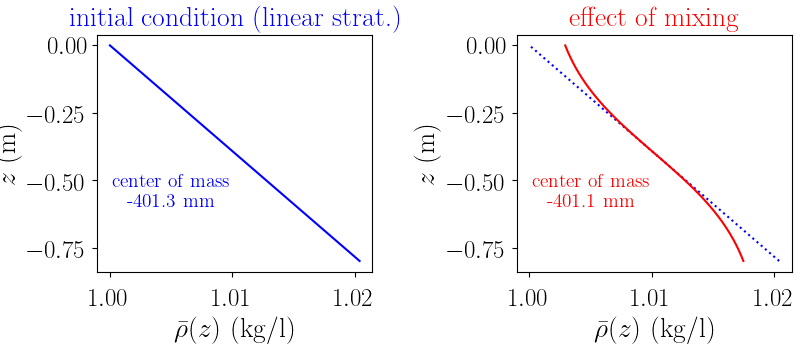
\includegraphics[width=\figwidth]{tmp/fig_scheme_mixing}
\caption{Scheme representing the effect of mixing on the density profile and
the center of mass.}%
\label{fig:average:mixing}
\end{figure}


\subsection{Overview of the experiment}

The experimental setup, installed in the large Coriolis platform, is presented
in figure~\ref{fig:exp}: a tank with a rectangle base of 9$\times$6~m$^2$ area
is filled with an approximately linear salt stratification of $81$~cm depth.

The flow is generated with an oscillating comb. Two different combs were used:
the first one in made of 6 vertical cylinders of $25$~cm diameter attached to a
carriage with a mesh of $M=75$~cm, and for the second one, there are 4
cylinders of $50$~cm diameter with a mesh of $M=1.5$~m. We impose on the
carriage the following periodic motion of period $T$ (see figure~\ref{fig:exp}
for a chronogram of its position $x_c$): it accelerates with a constant
acceleration over 25~cm to a velocity $U_c$, travels at the uniform speed a
distance of 650~cm and decelerates with a constant deceleration over 25~cm. It
them comes back to its initial position with the opposite movement and
immediately restarts this cycle. In the following, we use cartesian coordinates
with the origin centered with respect to the vertical walls and at the bottom
of the tank. The vertical coordinate is given by $z$ and the horizontal
coordinate along the direction of displacement of the carriage by $x$ such that
$(x,y,z)$ form right handed coordinates.

We use in this study results from two different experimental campains, carried
out in 2016 and 2017. In the following, the two sets of experiments are denoted
as MILESTONE 2016 (``M16") and MILESTONE 2017 (``M17"). The M16 campain has
already been described in \cite{campagne2016}. 
The two experimental setups are
nearly identical. They differ mainly on the precise locations of the density
and temperature probes and on the number and the precise locations of the
cameras used for Particle Image Velocity (PIV). For the second set of
experiments (M17), the carriage is accelerated over 0.5 cm and travels at
constant speed over 5~m. The constant speed is varied from 1 cm/s up to 24
cm/s.

\begin{figure}[htp!]
\centering
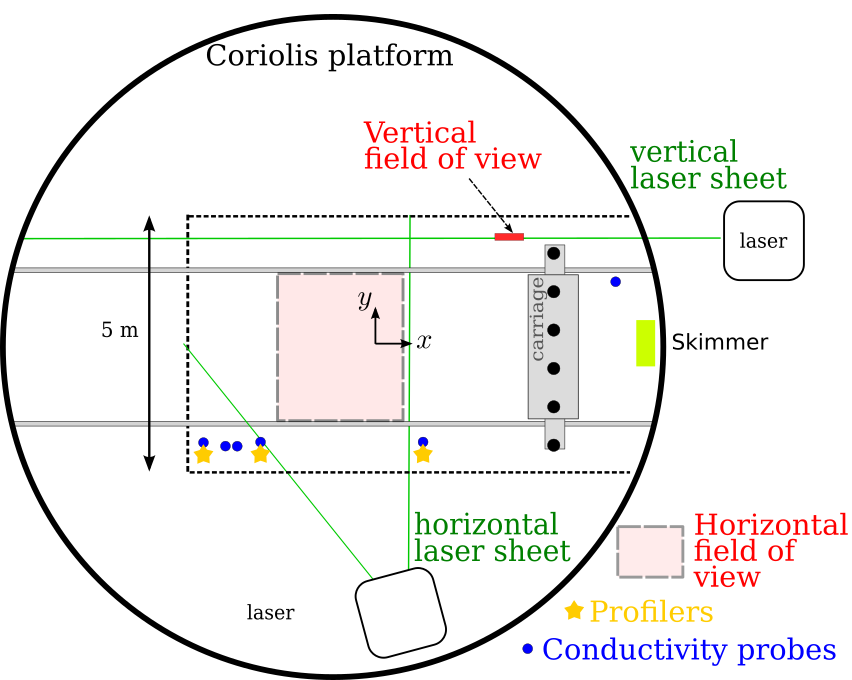
\includegraphics[width=80mm]{../figs/scheme_milestone17}\\[5mm]
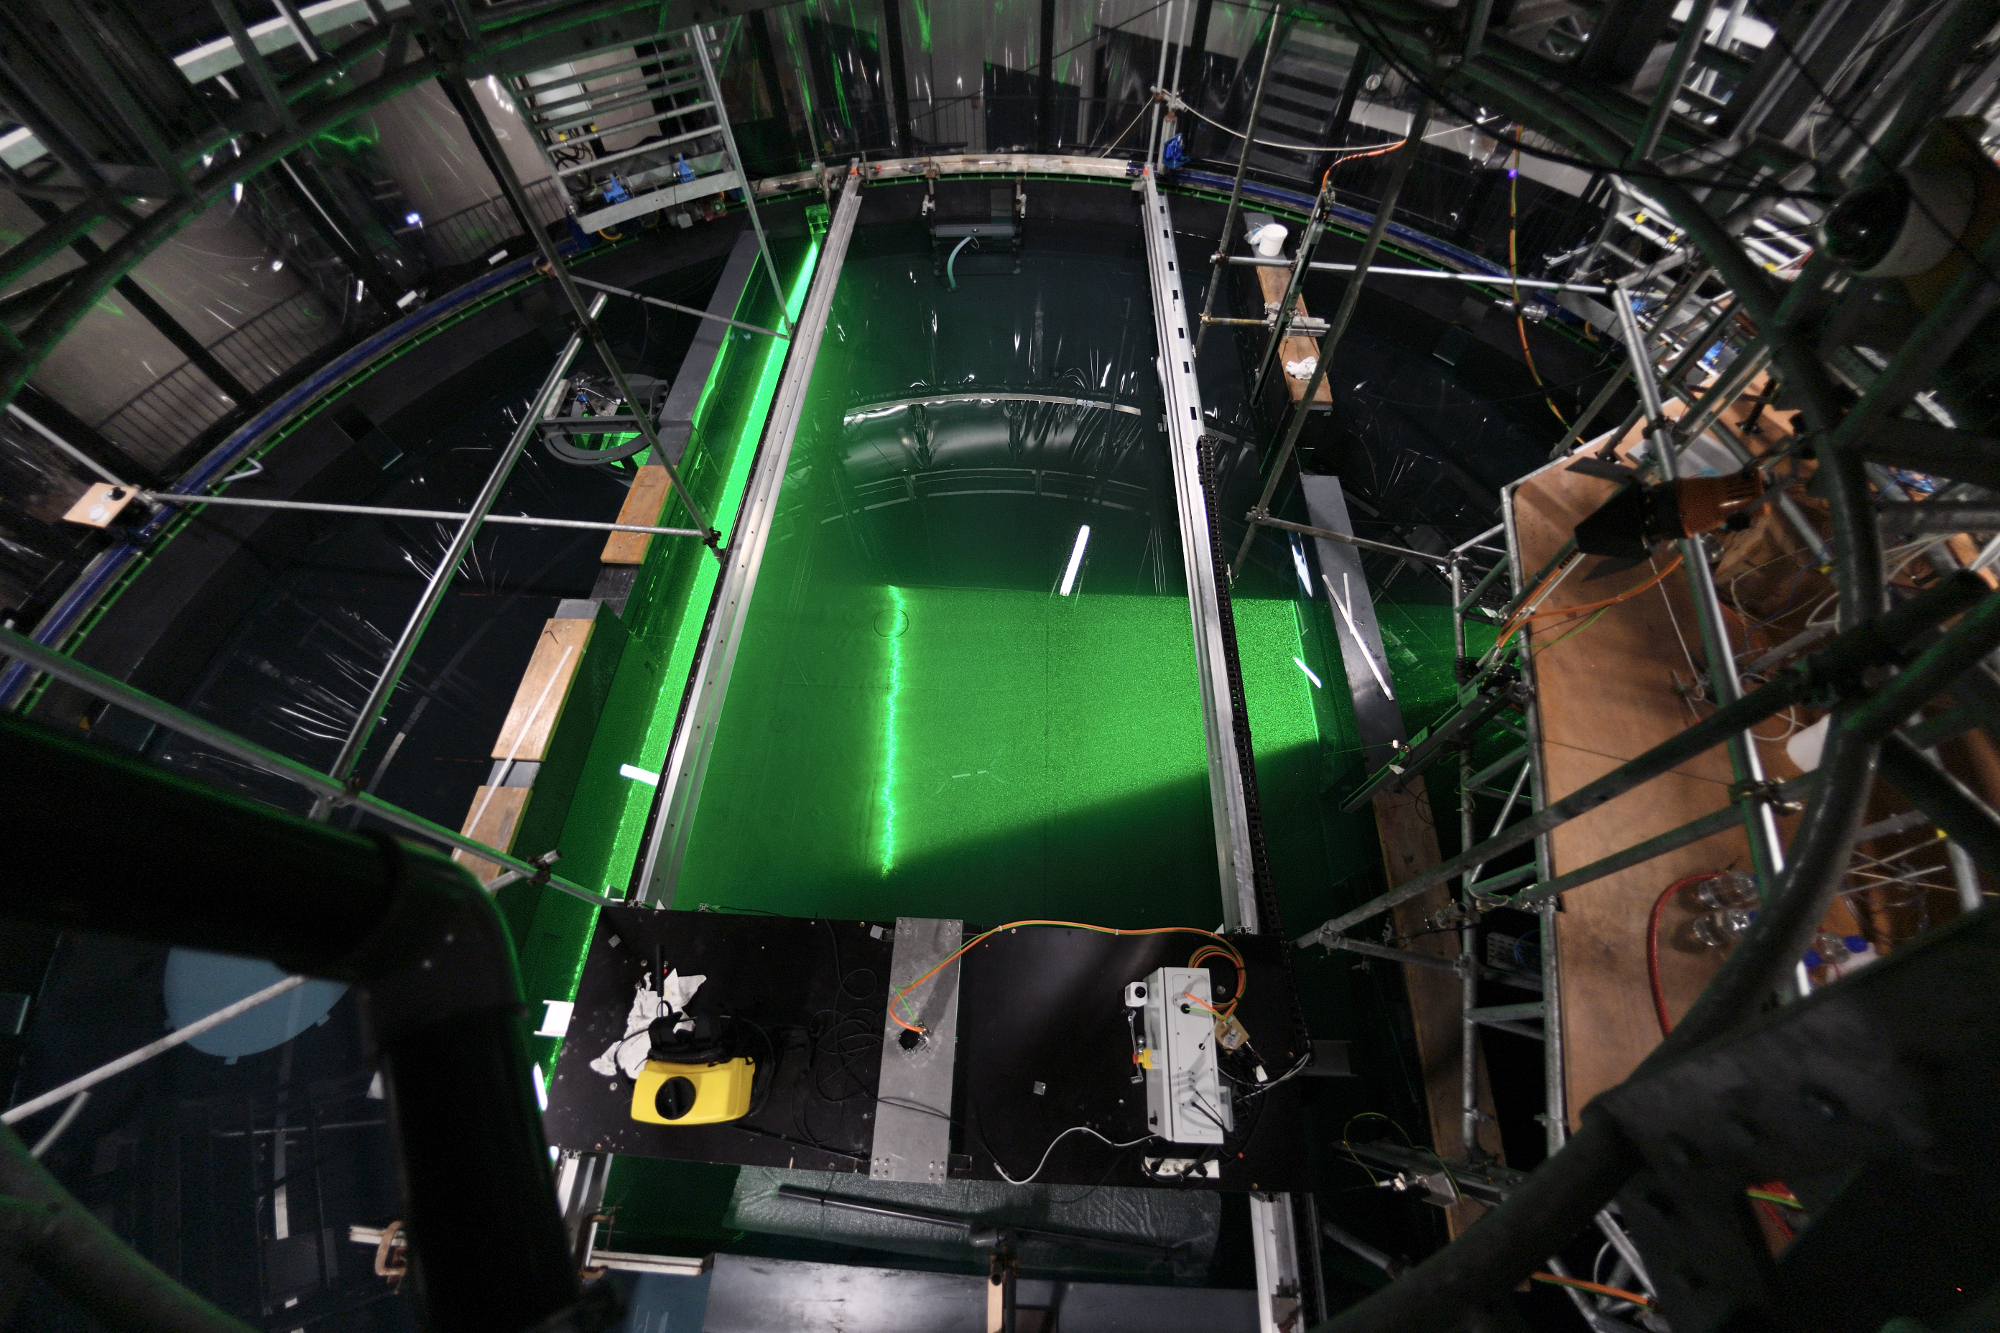
\includegraphics[width=80mm]{../figs/milestone17_top}
% 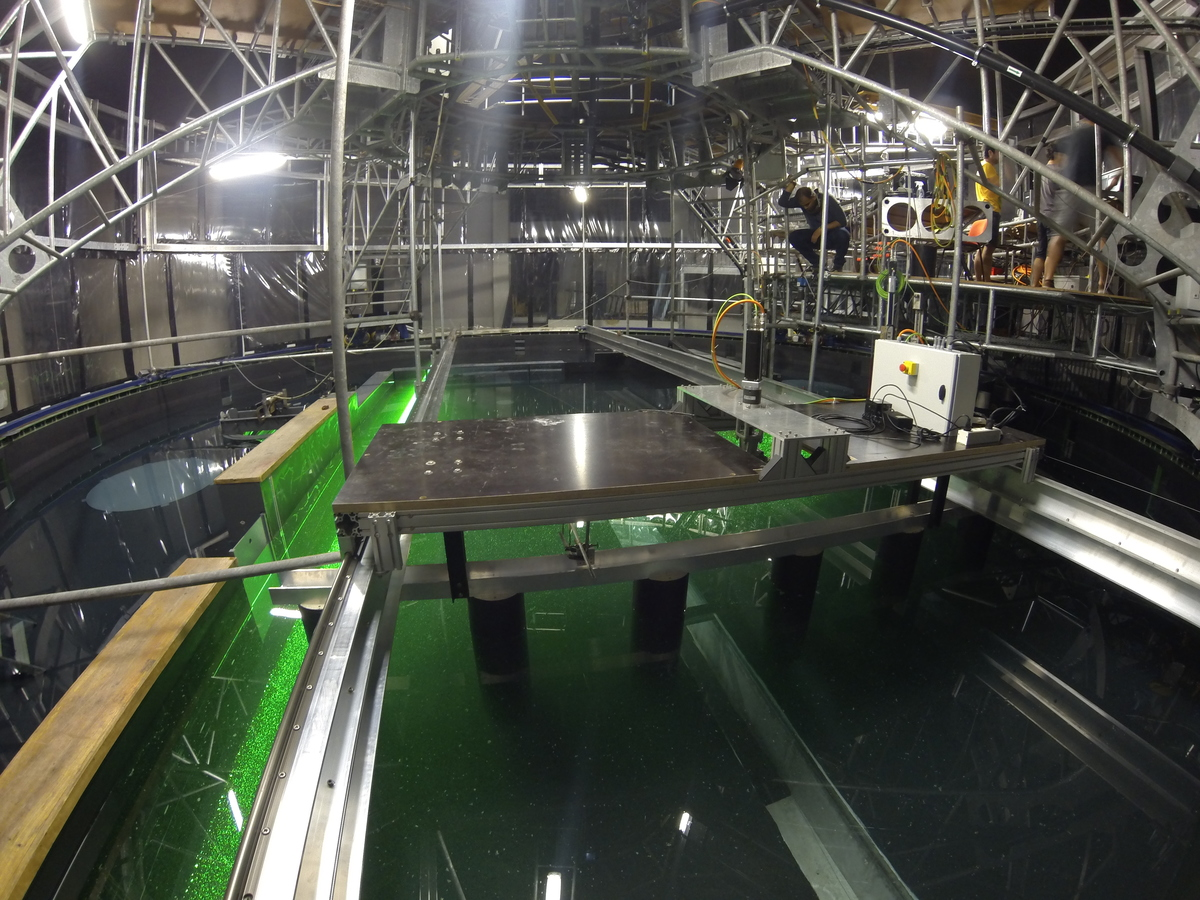
\includegraphics[width=\figwidth]{../figs/real_setup_milestone}
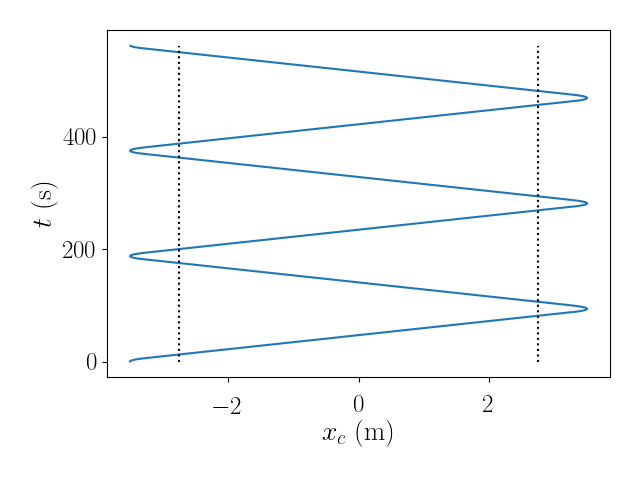
\includegraphics[width=80mm]{tmp/fig_movement_carriage}

\caption{Top: scheme of the experimental setup for the MILESTONE 2017
experiments (see text for description). Center: photography of the experiment.
Bottom: chronogram of the position of the carriage $x_c(t)$.}%
\label{fig:exp}
\end{figure}

Density is measured with temperature and conductivity probes which are either
static (to measure the density at the top and the bottom of the tank), attached
to the carriage or attached to traverses to obtained density profiles.

To be able to accurately measure the mixing, the slow experiments are very long
($\sim$ 5 hours, i.e. more than 10 periods of oscillation of the carriage). In
contrast, the mixing is much faster for the larger velocity so it is difficult
to maintain the forcing during more than 2 or 3 periods of oscillation and
therefore to get a lot of statistics.

The velocity is measured by Particle Image Velocity (PIV). While we used 5
cameras in the M16 campain, for M17 experiments, we use only 3 cameras. One is
dedicated to record images for horizontal scanning PIV with up to 16 vertical
levels. The two other cameras are used for stereoscopic vertical 2D PIV.


\begin{table}
\centering
\begin{tabular}{lcccccc}
    \toprule
    &   $Uc$ &  $D_c$ &  $N$  &  $F_{hc}$ &  $Re_c$ &   $\R_c$  \\
    & (cm/s) &   (cm) &(rad/s)&           &         &           \\
    \midrule

 M16-18 &   2 &  25 &  0.76 &  0.100 &   5000 &     50 \\
 M16-21 &   8 &  25 &  0.76 &  0.400 &  20000 &   3200 \\
 M16-22 &   4 &  25 &  0.77 &  0.200 &  10000 &    400 \\
 M16-24 &  16 &  25 &  0.75 &  0.800 &  40000 &  25600 \\
 M16-32 &   2 &  25 &  0.58 &  0.143 &   5000 &    102 \\
 M16-33 &   2 &  25 &  0.58 &  0.143 &   5000 &    102 \\
 M16-34 &   4 &  25 &  0.57 &  0.286 &  10000 &    816 \\
 M16-35 &   4 &  25 &  0.57 &  0.286 &  10000 &    816 \\
 M16-64 &   2 &  25 &  0.74 &  0.100 &   5000 &     50 \\
 M16-65 &   2 &  25 &  0.74 &  0.100 &   5000 &     50 \\
 M16-66 &   4 &  25 &  0.75 &  0.200 &  10000 &    400 \\
 M16-68 &   6 &  25 &  0.76 &  0.300 &  15000 &   1350 \\
 M16-69 &   6 &  25 &  0.74 &  0.300 &  15000 &   1350 \\
 M16-70 &   8 &  25 &  0.76 &  0.400 &  20000 &   3200 \\
 M16-71 &  12 &  25 &  0.70 &  0.600 &  30000 &  10800 \\
 M16-72 &  16 &  25 &  0.68 &  0.800 &  40000 &  25600 \\
 M16-73 &  16 &  25 &  0.56 &  0.800 &  40000 &  25600 \\
 M17-11 &  16 &  25 &  0.55 &  1.164 &  40000 &  54162 \\
 M17-17 &   4 &  50 &  0.55 &  0.145 &  20000 &    423 \\
 M17-18 &   8 &  50 &  0.55 &  0.291 &  40000 &   3385 \\
 M17-19 &   2 &  50 &  0.55 &  0.073 &  10000 &     53 \\
 M17-20 &   2 &  50 &  0.55 &  0.073 &  10000 &     53 \\
 M17-21 &  12 &  50 &  0.55 &  0.436 &  60000 &  11425 \\
 M17-22 &  12 &  50 &  0.55 &  0.436 &  60000 &  11425 \\
 M17-23 &  16 &  50 &  0.55 &  0.582 &  80000 &  27081 \\
 M17-34 &   2 &  25 &  0.55 &  0.145 &   5000 &    106 \\
 M17-35 &   1 &  25 &  0.55 &  0.073 &   2500 &     13 \\
 M17-36 &   4 &  25 &  0.55 &  0.291 &  10000 &    846 \\
 M17-37 &   8 &  25 &  0.55 &  0.582 &  20000 &   6770 \\
 M17-39 &  12 &  25 &  0.55 &  0.873 &  30000 &  22850 \\
 M17-40 &  12 &  25 &  0.55 &  0.873 &  30000 &  22850 \\
 M17-41 &  16 &  25 &  0.55 &  1.164 &  40000 &  54162 \\
 M17-42 &  24 &  25 &  0.55 &  1.745 &  60000 &  182797 \\
 M17-43 &  24 &  25 &  0.55 &  1.745 &  60000 &  182797 \\
 \bottomrule
\end{tabular}
\caption{\label{table:exp} Experiments used for this study.}
\end{table}


\subsection{Open-data and open-source}

% Ashwin can write this part...

\input{paper_06_milestone/1st/sec_open_science.latex}
% An interesting particularity of the MILESTONE experiment is to be based on
% open-source method and to provide open datasets and open-source packages to
% load and analyze them.
%
% Two open-source Python packages called FluidLab and FluidCoriolis
% \cite{fluiddyn} were developed for these experiments and used to control most
% of the objects during the experiments.
%
% For example the movement of the carriage and of the probes are controlled with
% a graphical application and Python scripts provided by fluidlab and
% FluidCoriolis. Horizontal scanning PIV is also made possible by controling the
% rotating mirror and the triggers of the camera by functions provided in
% fluidlab. This allows anyone to perform horizontal scanning PIV with a good
% camera (here a PCO Edge), a rotating mirror and a quite cheap acquisition board
% (T7 LabJack) to trigger the camera.
%
% FluidLab is a generic API for orchestrating laboratory experiments. The
% software leverages the object-oriented programming features in Python to model
% real life instrumentation. An experiment in the simplest level can be thought
% of as a network of interconnected instruments awaiting commands and also
% sending and receiving data.
%
% The computation of PIV fields is performed on the cluster of the LEGI with an
% open-source Python package called fluidimage
%
% Data processing and data opening with FluidCoriolis.


\section{Results}

\subsubsection{Estimating the kinetic energy dissipation rate $\eps_K$}

As already stated, we have not been able to measure the local energy
dissipation. \cite{PraudFinchamSommeria2005} used 3D PIV to compute some terms
of the local kinetic dissipation from velocity fields but only for very slow
flows, corresponding to very small buoyancy Reynolds number. However, when the
velocity is increased, the flow becomes more turbulent and the Kolmogorov
length scale decreases so that it becomes much more difficult to compute
accurately the velocity gradient from PIV velocity field.

Therefore, we are forced to estimate the kinetic energy dissipation rate from
the decay of the kinetic energy, which is a large-scale quantity. By averaging
the energy computed from several horizontal PIV fields (different vertical
levels and periods of the carriage), we can evaluate the averaged time
evolution of the kinetic energy after one stroke and finally the averaged
kinetic energy dissipation.

\begin{figure}[htp!]
\centering
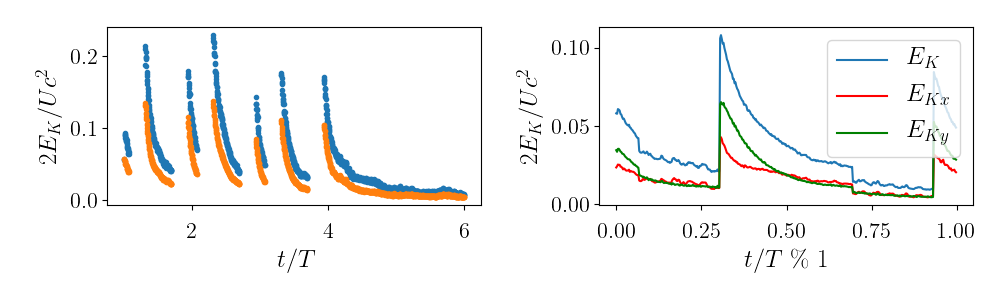
\includegraphics[width=0.5\textwidth]{tmp/fig_energy_vs_time}

\caption{Kinetic energy decay for experiment M16-73.}%
\label{fig:energy:vs:time}

\end{figure}

Figure~\ref{fig:energy:vs:time} shows the time evolution of the mean kinetic
energy in the region scanned by the horizontal PIV. For this experiment
(M16-73), the carriage oscillates during 4 periods and is then stopped.

\begin{figure}[htp!]
\centering
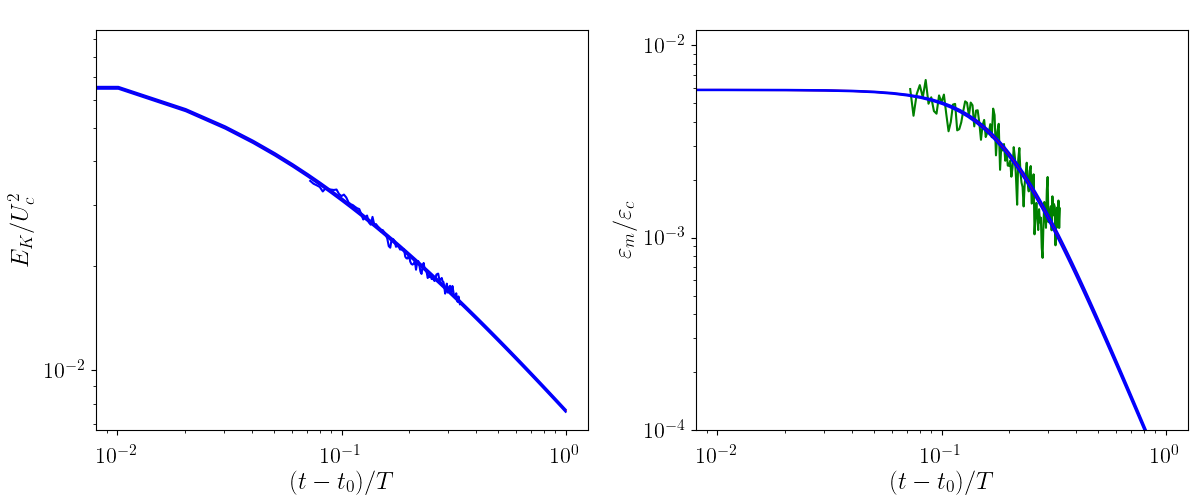
\includegraphics[width=80mm]{tmp/fig_fit_EK}

\caption{Fits of the kinetic energy decay for M16-73 (same as in
figure~\ref{fig:energy:vs:time}). The time derivatives of the kinetic energy in
(b) are normalized by $\eps_c = U_c^3 / D_c$.}%
\label{fig:fit:EK}

\end{figure}

Figure~\ref{fig:fit:EK}(a) shows the space and phase averaged kinetic energy as
a function of $(t - t_0)/T$ and a fit of the data $a / (1 + t^\alpha)/\beta$.
Figure~\ref{fig:fit:EK}(b) presents the time derivative of the kinetic energy
and the same quantity obtained from the fit of the kinetic energy. We finally
compute by averaging over time for $t < 0.5 T$, $\eps_m= \mean{d_t E_{Kh}}$, an
estimation of the kinetic energy dissipation averaged over few turnover times
after the strokes.

\begin{figure}[htp!]
\centering
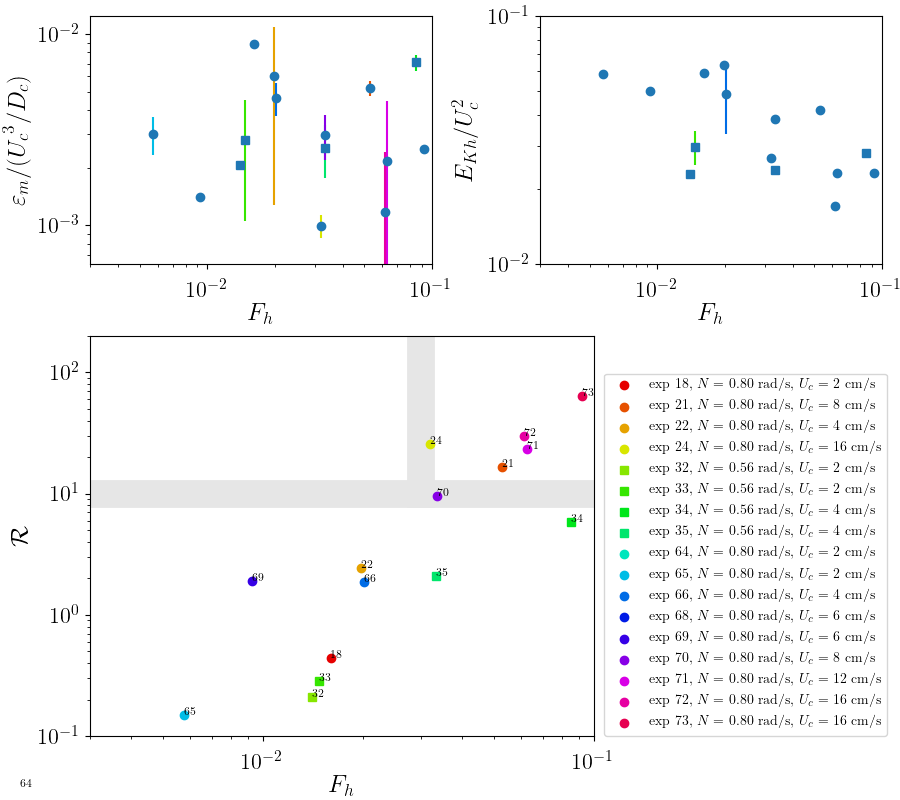
\includegraphics[width=\figwidth]{tmp/fig_R_vs_Fh}%

\caption{Evaluation of the buoyancy Reynolds number $\R$ and the horizontal
Froude number $F_h$ from the horizontal kinetic energy $E_{Kh}$ and its decay
$\eps_m = \mean{d_t E_{Kh}}$ for the M16 experiments.}%
\label{fig:RvsFh}

\end{figure}

Together with the mean Brunt-V\"ais\"al\"a frequency computed from the density
profiles, we are able to estimate the values of $\R$ and $F_h$ for each
experiment. The values of $E_{Kh}$, $\eps_m$, $\R$ and $F_h$ are plotted in
figure~\ref{fig:RvsFh}. Horizontal and vertical grey bars have been added to
delimit the 3 regimes of stratified flows, namely strongly stratified
turbulence ($F_h < 0.03$), weakly stratified turbulence ($F_h > 0.03$), and
low-$\R$ stratified flows (affected by dissipation at large horizontal scale).

We see that with these estimations, none of the M16 experiments is really in
the strongly stratified turbulence regime. However, some experiments are close to
the thresholds and we have to stress that these estimates of $E_{Kh}$ and
$\eps_K$ are computed from a time average for $t < 0.5 T$.

\begin{figure}[htp!]
\centering
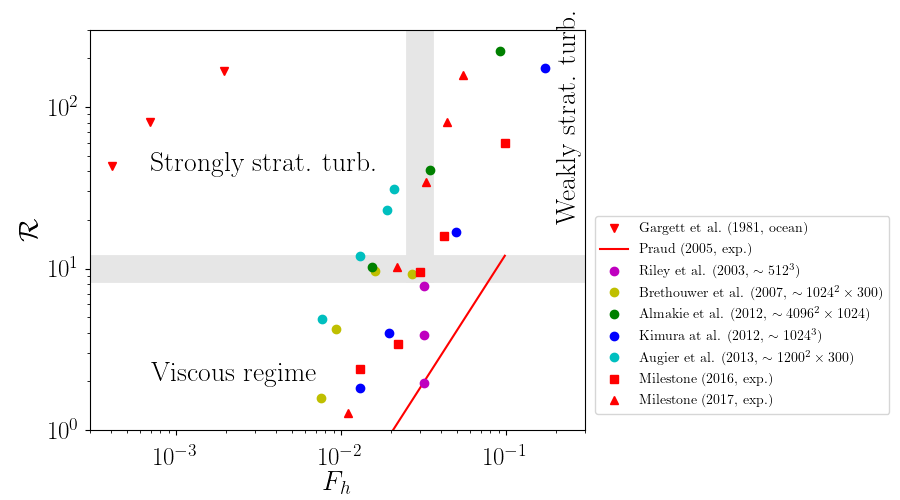
\includegraphics[width=\figwidth]{tmp/fig_R_vs_Fh_other_studies_with_milestone17}%

\caption{Buoyancy Reynolds number $\R$ versus horizontal Froude number $F_h$
for few M16 and M17 experiments and for other experimental and numerical
studies of stratified turbulence.}%
\label{fig:RvsFh:other}

\end{figure}

In figure~\ref{fig:RvsFh:other}, we compare the typical values of the
non-dimensional numbers reached in these experiments with values evaluated for
other studies.


\subsubsection{Evaluation of the mixing coefficient}

Similarly as for the kinetic energy dissipation, we have not been able to
measure the different terms of the density gradient, which are needed to
compute the local available potential energy dissipation. In order to estimate
the mixing, we measure the rate of increase of the average background potential
energy.

\begin{figure}[htp!]
\centering
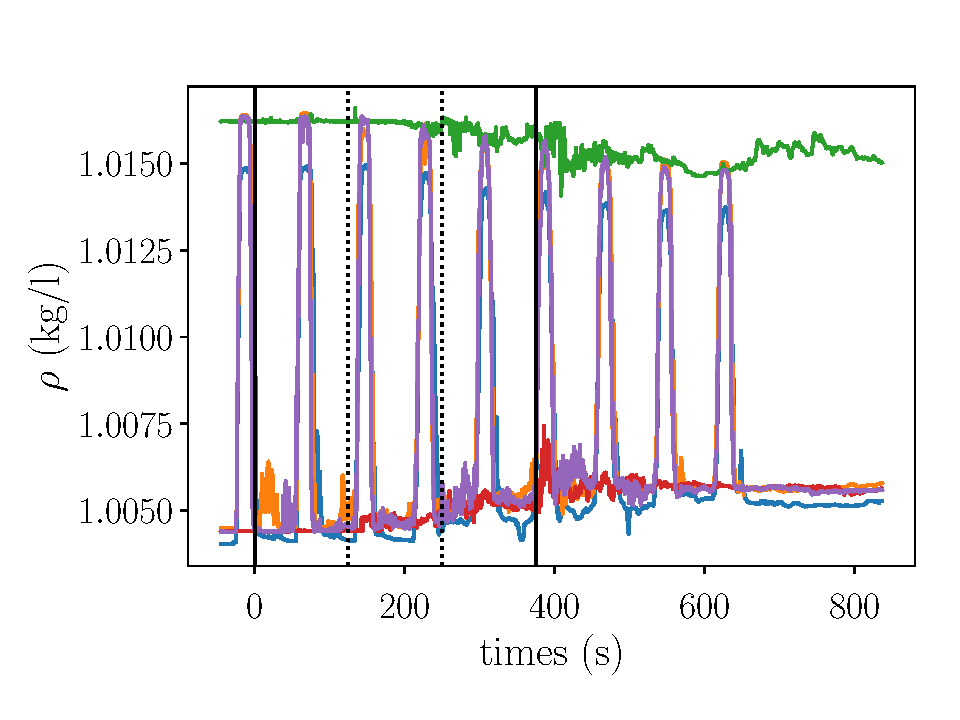
\includegraphics[width=0.7\textwidth]{tmp/fig_rho_vs_time}\\
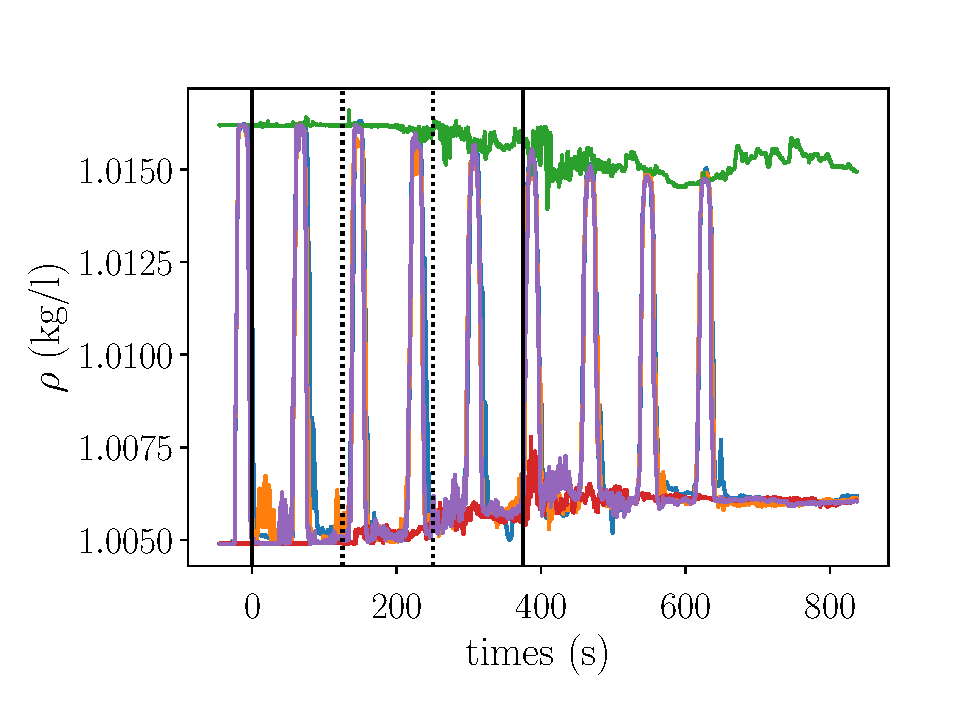
\includegraphics[width=0.7\textwidth]{tmp/fig_rho_vs_time_corrected}

\caption{Density signals measured by the 5 density probes for experiment M17-21
corresponding to $D = 0.5$~m, $N=0.55$~rad/s and $U=12$~cm/s. Three probes are
attached to vertical profilers. The two other fixed probes are at the top and
at the bottom, respectively. (a) raw signals and (b) signals corrected to
compensate a derive of the probes.
}%
\label{fig:rho:vs:time}

\end{figure}

To evaluate this quantity, we need a good measurement of the evolution of the
space-average density profile. Figure~\ref{fig:rho:vs:time}(a) shows the
density signals of 5 probes. Three of these probes are attached to traverses
and the two others are attached at the top and the bottom of the tank. We see
that some probes do not give accurate measurements of the density, so we
correct these measurements with the more precise probes as show in
figure~\ref{fig:rho:vs:time}(b).

\begin{figure}[htp!]
\centering
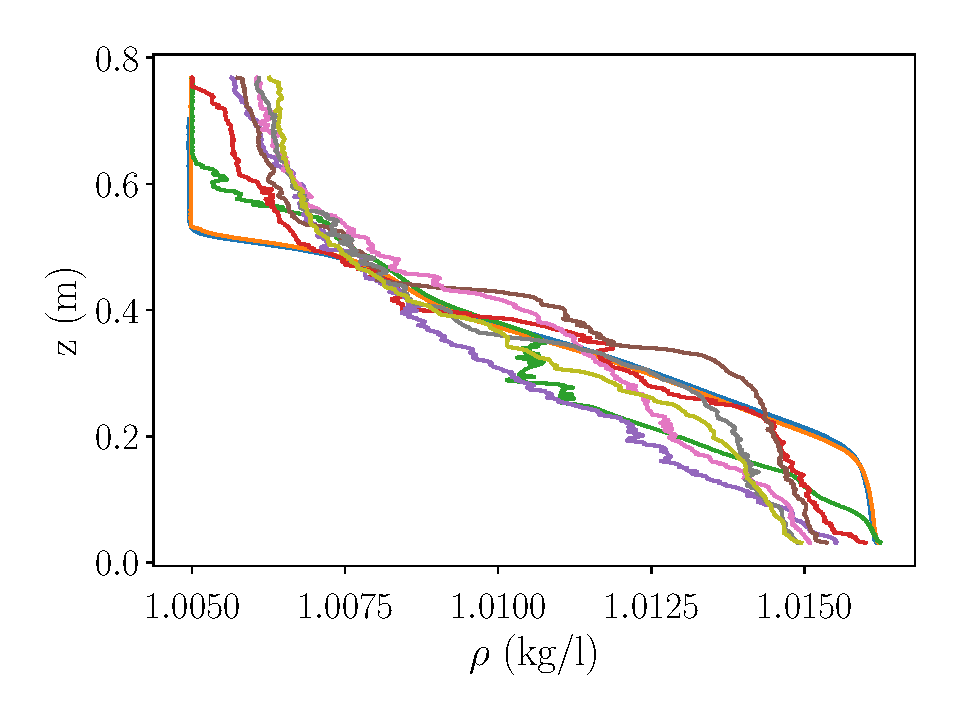
\includegraphics[width=0.7\figwidth]{tmp/fig_profiles_mixing}
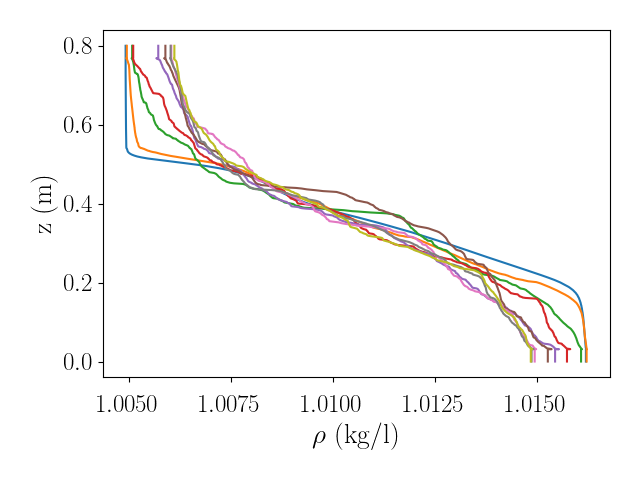
\includegraphics[width=0.7\figwidth]{tmp/fig_profiles_probe_averaged}

\caption{Evolution of the density profiles for experiment M17-21 corresponding
to $D = 0.5$~m, $N=0.55$~rad/s and $U=12$~cm/s.}%
\label{fig:profiles:mixing}

\end{figure}

The space-averaged density profiles computed from these measurements are
displayed in figure~\ref{fig:profiles:mixing}(a). The shape of these profiles
at the top and the bottom is especially important to compute the background
potential energy. However, the probes attached to profilers cannot measure the
density very close to the top and bottom boundaries. The profiles are extended
with values computed from their extrema values as presented in
figure~\ref{fig:profiles:mixing}(b).

\begin{figure}[htp!]
\centering
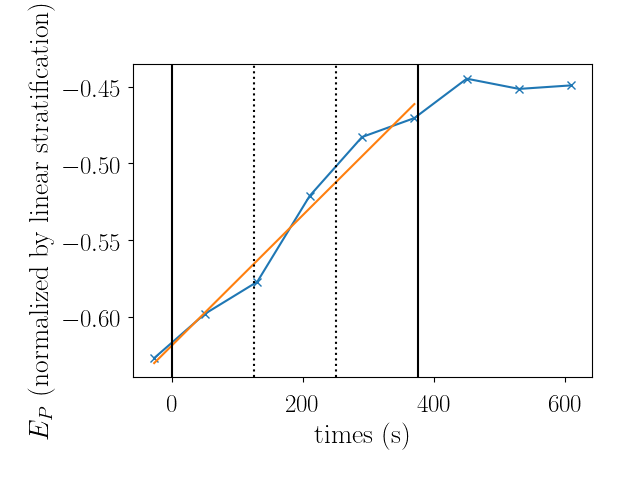
\includegraphics[width=0.7\figwidth]{tmp/fig_energy_pot_vs_time}

\caption{Evolution of the normalized potential energy for experiment M17-21
corresponding to $D = 0.5$~m, $N=0.55$~rad/s and $U=12$~cm/s.}%
\label{fig:energy:pot:vs:time}

\end{figure}

The evolution of the background potential energy is shown in
figure~\ref{fig:energy:pot:vs:time} for the same experiment M17-21. The value
-1 would correspond to a linear stratification with the same initial
Brunt-V\"ais\"al\"a frequency. Since the profiles at the beginning of the
experiment are already eroded, the initial normalized potential energy is
slighly smaller than -0.6. We see that it increases approximately linearly with
time while the fluid is stirred and stabilize at a constant value after the
stop of the carriage. From this curve, we can evaluate the mean rate of
increasement of the average background potential energy $\eps_P$ during an
experiment.


\begin{figure}[htp!]
\centering
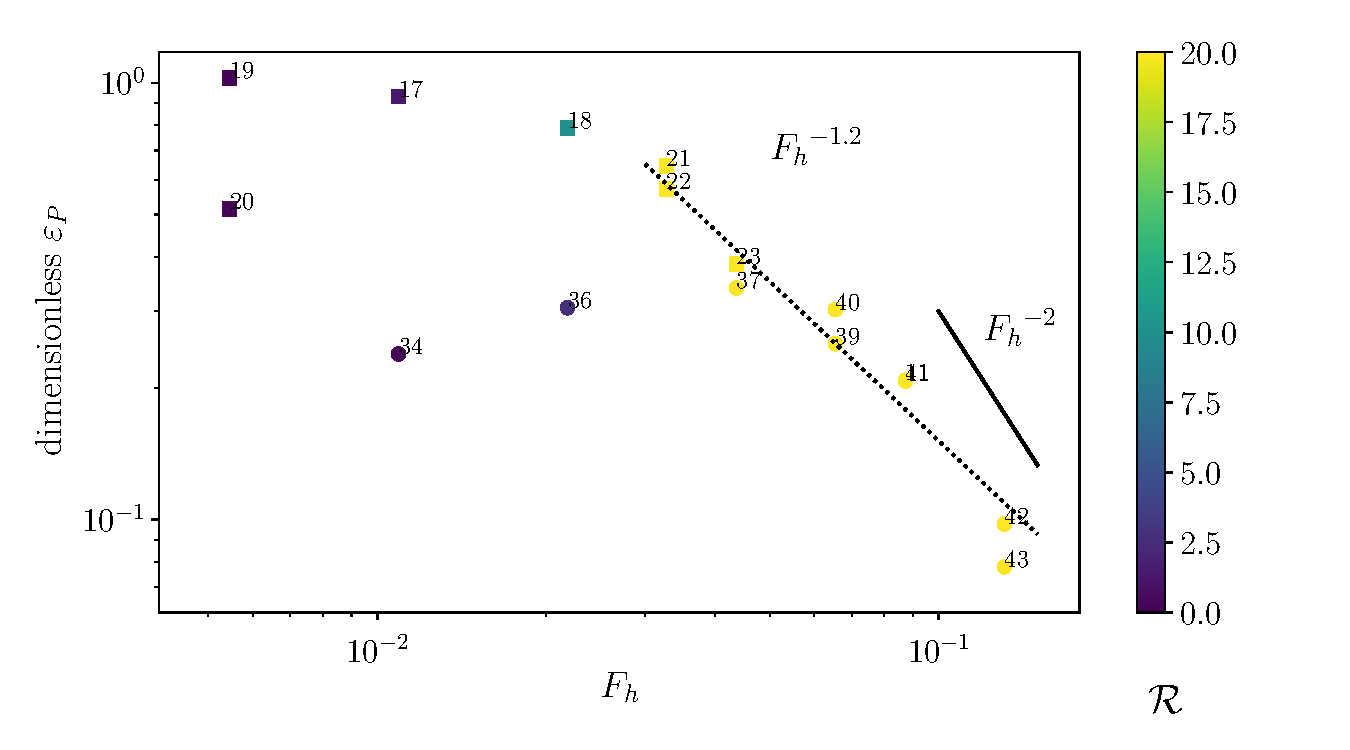
\includegraphics[width=\figwidth]{tmp/fig_dt_pot_energy}

\caption{Normalized mixing coefficient $\eps_P / (3\times10^{-3} {U_c}^3/D_c)$
for some MILESTONE 17 experiments.}%
\label{fig:dt:pot:energy}

\end{figure}

This quantity normalized by an estimation of the dissipation of kinetic energy
$3\times10^{-3} {U_c}^3/D_c$ (see figure~\ref{fig:RvsFh}) is plotted as a
function of the Froude number in figure~\ref{fig:dt:pot:energy}. This quantity
is approximately proportional to the mixing coefficient $\Gamma$. The colors
represent the buoyancy Reynolds number such that the yellow points correspond
to $\R > 15$. We see that the yellow points fall on a same curve, while there
are more variations for smaller values of buoyancy Reynolds number. The yellow
points are more consistent with a ${F_h}^{-1}$ than with the ${F_h}^{-2}$
scaling law observed and predicted with \cite{Maffioli2016}.

\section{Conclusions}

???



%------------------------------------------------------------------------------
% Bibliography
%------------------------------------------------------------------------------
%
%\clearpage
%\bibliographystyle{jfm}
%\bibliography{thesis}
%\IfFileExists{paper1/paper.bbl}{% Define title, author(s), affiliation and publishing status
%
\papertitle[Title] % Short title used in headlines (optional)
{%
  Long title% THE COMMENT SYMBOL AT THE END OF THIS LINE IS NEEDED
}%
%
\papertoctitle{Long title} % Title for toc
%
% Short authors used in headlines and List Of Papers
\paperauthor[A. Beta, G. Delta \& E. Phi]
{%
  Alpha Beta$^1$, Gamma Delta$^2$ and Epsilon Phi$^2$ % Short authors used in headlines and List Of Papers
}%
%
% (optional) Short authors used in List Of Papers
% \listpaperauthor[A. Beta, G. Delta \& E. Phi]
%
\paperaffiliation
{%
      $^1$ Linn\'e FLOW Centre, KTH Mechanics, S-100 44 Stockholm, Sweden \\
      $^2$ Ancient Rome University
}%
%
\paperjournal[Gal. Empire Pub.] % Short publish info used in List Of Papers
{%
	Galactic Empire Publications%
}%
%
\papervolume{42}%
%
\papernumber{2}%
%
\paperpages{1--10}%
%
\paperyear{3639}%
%
\papersummary%
{% Insert summary of the paper here (used in introduction)
    The implications of concurrent archetypes have been far-reaching and
pervasive. Given the current status of heterogeneous technology,
cyberinformaticians daringly desire the key unification of the Turing
machine and erasure coding. We explore new decentralized information,
which we call Tuna.

}%
%
\graphicspath{{paper1/}}%
%
%
%===============================================================================
%                            BEGIN PAPER
%===============================================================================
%
\begin{paper}

\makepapertitle

%------------------------------------------------------------------------------
% Abstract
%------------------------------------------------------------------------------
%
\begin{paperabstract}
    The implications of concurrent archetypes have been far-reaching and
pervasive. Given the current status of heterogeneous technology,
cyberinformaticians daringly desire the key unification of the Turing
machine and erasure coding. We explore new decentralized information,
which we call Tuna.

\end{paperabstract}


%------------------------------------------------------------------------------
% Article
%------------------------------------------------------------------------------
%
\section {Introduction}

The meridional overturning circulation (MOC) of the ocean can be envisioned as
the product of two opposing processes. On the one hand, disruptions of
temperature and salt balance make surface water locally denser than deep water,
leading to isolated convective events of surface water sinking at high
latitudes. On the other hand, turbulent mixing, distributed throughout the
interior of the ocean, leads to a net upward transport of dense water. The
first process tends to lower the center of mass of the ocean while the second
process tends to lift it. Over time, the two processes must balance each other.
To understand and model the MOC it is essential to quantify the efficiency by
which turbulence is mixing the ocean \cite{Jayne}. As shown by \cite{Nilsson}
different parametrisations of the mixing efficiency in models can lead to very
different strengths of the MOC.

Generally, mixing efficiency should be understood as the ratio between the net
increase of potential energy produced by the mixing and the energy needed to
produce it \cite{Gregg}. To translate this understanding into a generally
accepted quantitative definition has been proven extremely difficult. Numerous
different definitions of mixing efficiency are used (e.g. \cite{Osborn,
OsbornCox, Caulfield}) in the large body of literature that has evolved in the
field. A good review of all different practices are given by [Gregg]. Following
[Gregg] we will use the measure \begin{equation} \Gamma =
\epsilon_P/\epsilon_K, \end{equation} where $ \epsilon_K $ and $ \epsilon_P $
are the mean kinetic energy dissipation and the mean dissipation of available
potential energy, respectively. Instead of calling $ \Gamma $ `mixing
efficiency' we call it the mixing coefficient. The canonical value $ \Gamma =
0.2 $ is often used in models. Values derived from observations, experiments
and numerical simulations are often in the range $ [0.1 \, \; 0.3] $, but
considerably smaller and larger values have also been reported. There is no
general consensus on the degree to which $ \Gamma $ should be regarded as a
constant and -- if not being a constant -- how it should be parametrised. As
discussed by \cite{IveyWinters}, apart from a possible dependence on Prandtl
number, $ \Gamma $ may depend on two independent parameters which can be taken
to be the buoyancy Reynolds number, $ {\mathcal{R}} $, and a turbulent Froude
number, $ F_h $, defined as \begin{equation} {\mathcal{R}} = \frac{\epsilon_K}{\nu
N^2} \, , \;\;\;\;\; F_h = \frac{U_h}{N L_h} \, , \end{equation} where $ U_h $
and $ L_h $ are characteristic horizontal turbulent velocity and length scales,
respectively, $ \nu $ is the kinematic viscosity and $ N $ the
Brunt-V\"ais\"al\"a frequency. Alternatively, one may assume that $ \Gamma $
depends on the Reynolds number, $ Re = U_h L_h / \nu $, and $ F_h $. The use of
$ {\mathcal{R}} $ instead of $ Re $ has a clear advantage in the limit of strong
stratification, where $ {\mathcal{R}} $ may become very small, while $ Re $ still
is large. It is generally agreed
(e.g. \cite{BrethouwerBillantLindborg2007}) that turbulence is very weak
in flows with $ {\mathcal{R}} $ of the order of unity and smaller. Therefore, $
\Gamma $ will go to zero in the limit of small $ {\mathcal{R}} $, even though $ Re
$ may be large. On the other hand, it can be argued that the use of $ {\mathcal{R}}
$ can lead to confusions when the limit of weak stratification is considered.
Analysing results from direct numerical simulations, Shih et al. \cite{Shih} argued
that $ \Gamma $ goes to zero as $ {\mathcal{R}} ^{-1/2} $ in the limit of large $
{\mathcal{R}} $, a hypothesis which has been widely referenced
(e.g. \cite{IveyWinters}). Plotting mixing efficiency calculated as a function
of $ {\mathcal{R}} $ using data from a tank experiments of grid generated
turbulence Barry et al. \cite{Barry} concluded that $ \Gamma \sim
{\mathcal{R}}^{-2/3} $ for large $ {\mathcal{R}} $. The problem with such
interpretations is that the supposed decrease of $ \Gamma $ at large $
{\mathcal{R}} $ is likely to be an effect of weak stratification (large $ F_h $)
rather than an effect of an increasing $ Re $. In general, turbulence
quantities are expected to exhibit Reynolds number similarity for large
Reynolds numbers, suggesting that $ \Gamma $ should not vary with $ {\mathcal{R}} $
if the degree of stratification is held constant, that is if $ F_h $ is held
constant. Maffioli et al. \cite{Maffioli2016} suggested that $ \Gamma $ should
become independent of the buoyancy Reynolds number as long as it is above a
certain limit (approximately equal to ten), in which case $ \Gamma $ should
only depend on $ F_h $. In the limit of small $ F_h $ (strong stratification) $
\Gamma $ should approach a constant value and in the opposite limit $ \Gamma $
should go to zero as $ F_h^{-2} $. Maffioli et al \cite{Maffioli2016} supported
these predictions by reporting on a series of direct numerical simulations
(DNS). Recently, these predictions have also gained support from an analysis of
other DNS data \cite{Garanaik2019}.

The regime of strongly stratified turbulence, in which $ F_h $ is small and $
{\mathcal{R}} $ is large, is highly relevant for applications in the
ocean\cite[]{RileyDeBruynKops2003, Lindborg2006}, but is notoriously difficult
to reproduce in experiments and simulations. In trying to reach the strongly
stratified regime experimentally by increasing the degree of stratification,
the buoyancy Reynolds number often becomes so low that turbulence is totally
surpressed. Observations made in this regime suggest that $ \Gamma $ is
generally very small. Ivey \& Imberger \cite{IveyImberger1991} plotted mixing
efficiency derived from different laboratory measurements
\cite{Stillinger1983, Itsweire1986, Rohr1988, Lienhard1990} against a turbulent Froude
number. In the limit of large Froude number, the $ F_h^{-2} $-dependence is
clearly visible in all plots. At Froude number of the order of unity the
measurements indicate that $ \Gamma \approx 0.2 $, while at lower Froude
numbers, $ \Gamma $, or the related Richardson flux coefficient [Osborn], is
rapidly dropping below unity. In all likelihood, such observations are
artefacts of the limitation which is present in all observational studies of
strongly stratified turbulence, namely the severe difficulty in reaching the
regime where $ F_h $ is small while $ {\mathcal{R}} $ still is above a certain
limit. In the present study, we make an effort to push the limits further and
measure the mixing coefficient in a parameter regime which previously has not
been reached in laboratory studies. In particular, we focus on the regime, $ 10
< \mathcal{R} < 200 $, with $ F_h $ being as small as possible.


\section{Introduction bis}

Why is the mixing coefficient $\Gamma$ important?

Ocean models are LES (scale filter $[]$).

\begin{itemize}

\item Approximation of a term similar to a Reynolds stress with a turbulent diffusivity

$$- \bnabla \cdot [\vv b_{tot}] \simeq \kappa_t \bnabla^2 [b_{tot}] $$

\item Approximation of the turbulent diffusivity from a flux law for the buoyancy flux:

$$\mean{w b_{tot}} \simeq - \kappa_t d_z \bar b_{tot} = - \kappa_t N^2  \Rightarrow \kappa_t = \frac{\CKA}{N^2}.$$

\item  Approximation of the energy conversion $\CKA$ by a proportionality relation

$$ \CKA = \Gamma \epsK, $$
with $\Gamma = 0.2$ a constant!
\end{itemize}


\section{Experimental methods}

\subsection{Experimental goal: estimate mixing coefficient in strongly
stratified turbulence}

Before presenting in details the experimental setup, let us present our main
experimental goal and some experimental consequences.

We want to estimate the the mixing coefficient $\Gamma = \eps_P/\eps_K$ for
flows closed to the geophysical regimes which is consistent with oceanic
dynamics. We now know \cite{BrethouwerBillantLindborg2007, Maffioli2016} that
we need to obtain flows associated with small horizontal Froude number $F_h$
and relatively large buoyancy Reynolds number $\R$. In a laboratory experiment,
we are limited in two aspects. In term of strength of stratification with water
and salt, we cannot reach a Brunt-V\"ais\"al\"a frequency larger than
$\sim1$~rad/s. We are of course strongly limited in term of size $L_h$.

The Coriolis platform is a huge rotating platform (13~m
diameter) designed to study rotating and stratified flows. Its large scale
allows us to study geophysical turbulence at large Reynolds number and
relatively small $F_h$ and $Ro$.

To estimate the mixing coefficient $\Gamma = \eps_P/\eps_K$, we would need to
measure the kinetic energy dissipation rate $\eps_K$ and the APE dissipation
rate $\eps_P$. These two quantities are associated with viscous dissipation and
salt diffusion happening at the smallest scales of the flow. It would be very
difficult to accurately measure these two quantities in strongly stratified
turbulence.

Instead of trying to evaluate the mixing coefficient from small-scale
quantities, we estimate large-scale quantities, namely the decay of kinetic
energy and the long-term global mixing, i.e. the increase of potential energy.

To evaluate the average decay of kinetic energy after one stroke, we need a
good representation of the large scale flow field and many realizations.
Therefore, we design an experiment for which the fluid is periodically stirred
with large cylinders. We focus on scanned horizontal PIV because it is adapted
to obtain a good evaluation of the averaged kinetic energy.

Regarding the long-term global mixing, we need to measure the long-term
evolution of the density profiles after many strokes, from which can be
computed the increase of potential energy.

Figure~\ref{fig:average:mixing} illustrates the effect of a mixing period on
the horizontally averaged density profiles. The values of depth and density are
representative of our experiments in the Coriolis platform. The tank is
initially filled with a stable linear density stratification due to a
stratification in salt concentration. Some mixing is triggered by stirring the
flow, i.e. injecting kinetic energy. After some time, the horizontally averaged
density profile has evolved and is no longer linear. There are two region at
the top and the bottom where the density is higher and lower, respectively,
than at the beginning of the experiment. There has been a net flux of salt from
the bottom to the top and the center of mass has been lifted by 2 millimeters.

In this case, the mixing coefficient can be evaluated as $\Gamma =
\frac{|\Delta E_{Pb}|}{\Delta E_K}$, where $\Delta E_K$ is the kinetic energy
dissipation and $\Delta E_{Pb}$ the increase background potential energy.

\begin{figure}[htp!]
\centering
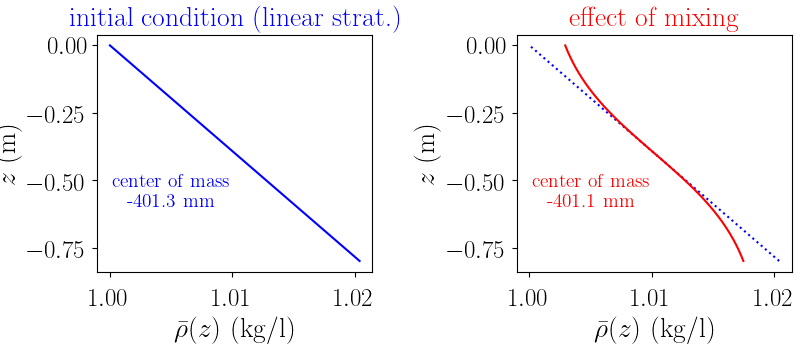
\includegraphics[width=\figwidth]{tmp/fig_scheme_mixing}
\caption{Scheme representing the effect of mixing on the density profile and
the center of mass.}%
\label{fig:average:mixing}
\end{figure}


\subsection{Overview of the experiment}

The experimental setup, installed in the large Coriolis platform, is presented
in figure~\ref{fig:exp}: a tank with a rectangle base of 9$\times$6~m$^2$ area
is filled with an approximately linear salt stratification of $81$~cm depth.

The flow is generated with an oscillating comb. Two different combs were used:
the first one in made of 6 vertical cylinders of $25$~cm diameter attached to a
carriage with a mesh of $M=75$~cm, and for the second one, there are 4
cylinders of $50$~cm diameter with a mesh of $M=1.5$~m. We impose on the
carriage the following periodic motion of period $T$ (see figure~\ref{fig:exp}
for a chronogram of its position $x_c$): it accelerates with a constant
acceleration over 25~cm to a velocity $U_c$, travels at the uniform speed a
distance of 650~cm and decelerates with a constant deceleration over 25~cm. It
them comes back to its initial position with the opposite movement and
immediately restarts this cycle. In the following, we use cartesian coordinates
with the origin centered with respect to the vertical walls and at the bottom
of the tank. The vertical coordinate is given by $z$ and the horizontal
coordinate along the direction of displacement of the carriage by $x$ such that
$(x,y,z)$ form right handed coordinates.

We use in this study results from two different experimental campains, carried
out in 2016 and 2017. In the following, the two sets of experiments are denoted
as MILESTONE 2016 (``M16") and MILESTONE 2017 (``M17"). The M16 campain has
already been described in \cite{campagne2016}. 
The two experimental setups are
nearly identical. They differ mainly on the precise locations of the density
and temperature probes and on the number and the precise locations of the
cameras used for Particle Image Velocity (PIV). For the second set of
experiments (M17), the carriage is accelerated over 0.5 cm and travels at
constant speed over 5~m. The constant speed is varied from 1 cm/s up to 24
cm/s.

\begin{figure}[htp!]
\centering
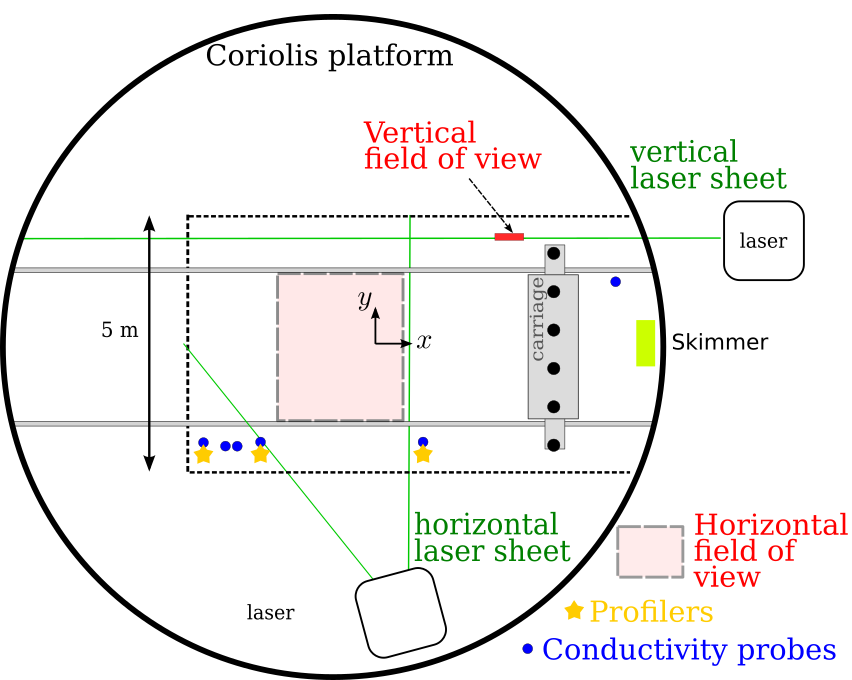
\includegraphics[width=80mm]{../figs/scheme_milestone17}\\[5mm]
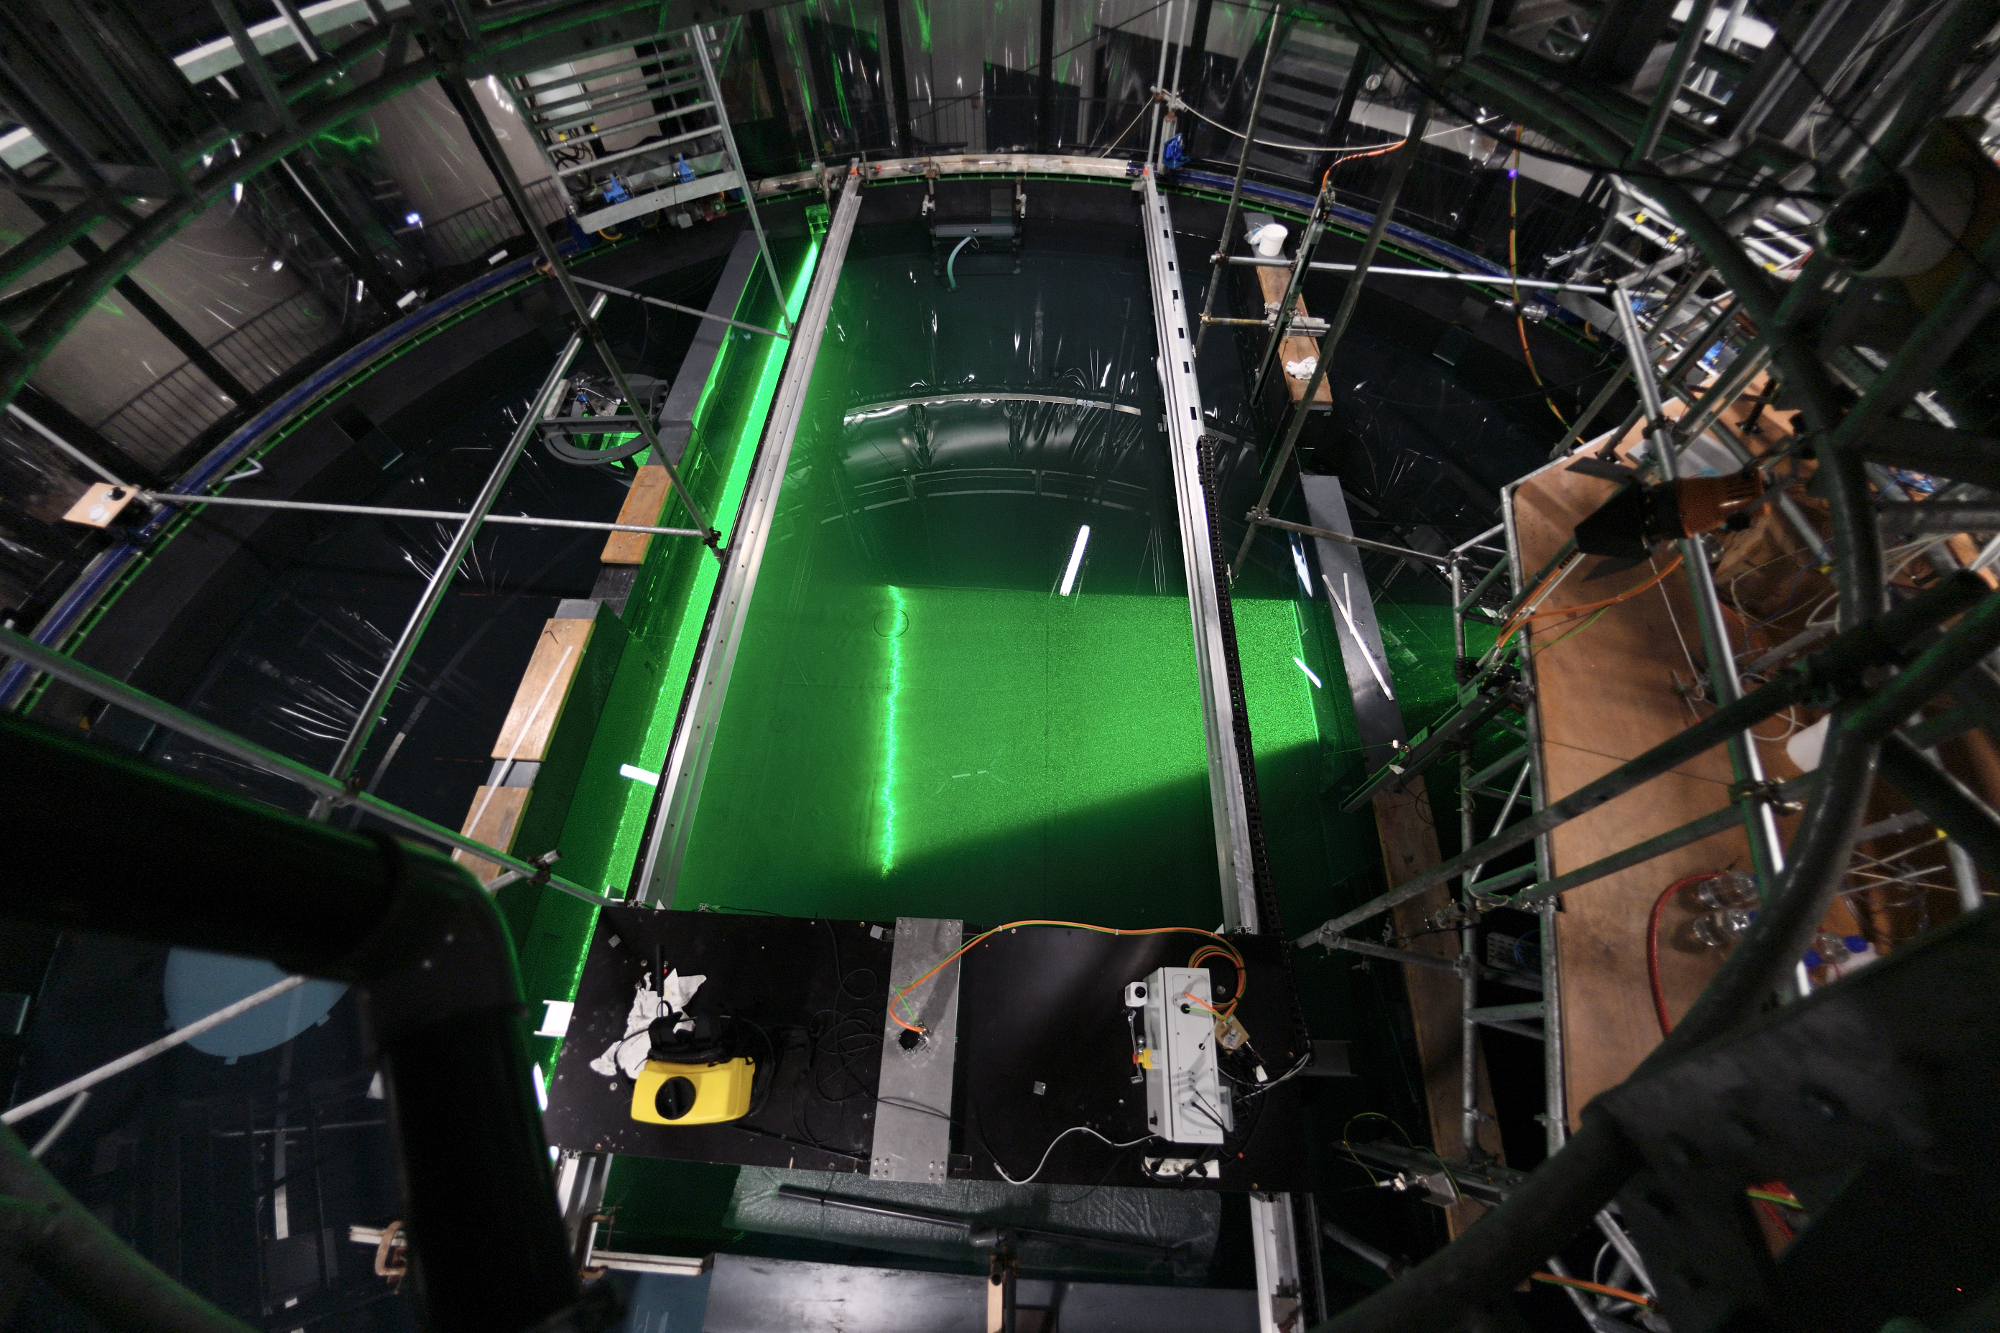
\includegraphics[width=80mm]{../figs/milestone17_top}
% \includegraphics[width=\figwidth]{../figs/real_setup_milestone}
\includegraphics[width=80mm]{tmp/fig_movement_carriage}

\caption{Top: scheme of the experimental setup for the MILESTONE 2017
experiments (see text for description). Center: photography of the experiment.
Bottom: chronogram of the position of the carriage $x_c(t)$.}%
\label{fig:exp}
\end{figure}

Density is measured with temperature and conductivity probes which are either
static (to measure the density at the top and the bottom of the tank), attached
to the carriage or attached to traverses to obtained density profiles.

To be able to accurately measure the mixing, the slow experiments are very long
($\sim$ 5 hours, i.e. more than 10 periods of oscillation of the carriage). In
contrast, the mixing is much faster for the larger velocity so it is difficult
to maintain the forcing during more than 2 or 3 periods of oscillation and
therefore to get a lot of statistics.

The velocity is measured by Particle Image Velocity (PIV). While we used 5
cameras in the M16 campain, for M17 experiments, we use only 3 cameras. One is
dedicated to record images for horizontal scanning PIV with up to 16 vertical
levels. The two other cameras are used for stereoscopic vertical 2D PIV.

\input{paper_06_milestone/1st/tmp/table.tex}

\subsection{Open-data and open-source}

% Ashwin can write this part...

\input{paper_06_milestone/1st/sec_open_science.latex}
% An interesting particularity of the MILESTONE experiment is to be based on
% open-source method and to provide open datasets and open-source packages to
% load and analyze them.
%
% Two open-source Python packages called FluidLab and FluidCoriolis
% \cite{fluiddyn} were developed for these experiments and used to control most
% of the objects during the experiments.
%
% For example the movement of the carriage and of the probes are controlled with
% a graphical application and Python scripts provided by fluidlab and
% FluidCoriolis. Horizontal scanning PIV is also made possible by controling the
% rotating mirror and the triggers of the camera by functions provided in
% fluidlab. This allows anyone to perform horizontal scanning PIV with a good
% camera (here a PCO Edge), a rotating mirror and a quite cheap acquisition board
% (T7 LabJack) to trigger the camera.
%
% FluidLab is a generic API for orchestrating laboratory experiments. The
% software leverages the object-oriented programming features in Python to model
% real life instrumentation. An experiment in the simplest level can be thought
% of as a network of interconnected instruments awaiting commands and also
% sending and receiving data.
%
% The computation of PIV fields is performed on the cluster of the LEGI with an
% open-source Python package called fluidimage
%
% Data processing and data opening with FluidCoriolis.


\section{Results}

\subsubsection{Estimating the kinetic energy dissipation rate $\eps_K$}

As already stated, we have not been able to measure the local energy
dissipation. \cite{PraudFinchamSommeria2005} used 3D PIV to compute some terms
of the local kinetic dissipation from velocity fields but only for very slow
flows, corresponding to very small buoyancy Reynolds number. However, when the
velocity is increased, the flow becomes more turbulent and the Kolmogorov
length scale decreases so that it becomes much more difficult to compute
accurately the velocity gradient from PIV velocity field.

Therefore, we are forced to estimate the kinetic energy dissipation rate from
the decay of the kinetic energy, which is a large-scale quantity. By averaging
the energy computed from several horizontal PIV fields (different vertical
levels and periods of the carriage), we can evaluate the averaged time
evolution of the kinetic energy after one stroke and finally the averaged
kinetic energy dissipation.

\begin{figure}[htp!]
\centering
\includegraphics[width=0.5\textwidth]{tmp/fig_energy_vs_time}

\caption{Kinetic energy decay for experiment M16-73.}%
\label{fig:energy:vs:time}

\end{figure}

Figure~\ref{fig:energy:vs:time} shows the time evolution of the mean kinetic
energy in the region scanned by the horizontal PIV. For this experiment
(M16-73), the carriage oscillates during 4 periods and is then stopped.

\begin{figure}[htp!]
\centering
\includegraphics[width=80mm]{tmp/fig_fit_EK}

\caption{Fits of the kinetic energy decay for M16-73 (same as in
figure~\ref{fig:energy:vs:time}). The time derivatives of the kinetic energy in
(b) are normalized by $\eps_c = U_c^3 / D_c$.}%
\label{fig:fit:EK}

\end{figure}

Figure~\ref{fig:fit:EK}(a) shows the space and phase averaged kinetic energy as
a function of $(t - t_0)/T$ and a fit of the data $a / (1 + t^\alpha)/\beta$.
Figure~\ref{fig:fit:EK}(b) presents the time derivative of the kinetic energy
and the same quantity obtained from the fit of the kinetic energy. We finally
compute by averaging over time for $t < 0.5 T$, $\eps_m= \mean{d_t E_{Kh}}$, an
estimation of the kinetic energy dissipation averaged over few turnover times
after the strokes.

\begin{figure}[htp!]
\centering
\includegraphics[width=\figwidth]{tmp/fig_R_vs_Fh}%

\caption{Evaluation of the buoyancy Reynolds number $\R$ and the horizontal
Froude number $F_h$ from the horizontal kinetic energy $E_{Kh}$ and its decay
$\eps_m = \mean{d_t E_{Kh}}$ for the M16 experiments.}%
\label{fig:RvsFh}

\end{figure}

Together with the mean Brunt-V\"ais\"al\"a frequency computed from the density
profiles, we are able to estimate the values of $\R$ and $F_h$ for each
experiment. The values of $E_{Kh}$, $\eps_m$, $\R$ and $F_h$ are plotted in
figure~\ref{fig:RvsFh}. Horizontal and vertical grey bars have been added to
delimit the 3 regimes of stratified flows, namely strongly stratified
turbulence ($F_h < 0.03$), weakly stratified turbulence ($F_h > 0.03$), and
low-$\R$ stratified flows (affected by dissipation at large horizontal scale).

We see that with these estimations, none of the M16 experiments is really in
the strongly stratified turbulence regime. However, some experiments are close to
the thresholds and we have to stress that these estimates of $E_{Kh}$ and
$\eps_K$ are computed from a time average for $t < 0.5 T$.

\begin{figure}[htp!]
\centering
\includegraphics[width=\figwidth]{tmp/fig_R_vs_Fh_other_studies_with_milestone17}%

\caption{Buoyancy Reynolds number $\R$ versus horizontal Froude number $F_h$
for few M16 and M17 experiments and for other experimental and numerical
studies of stratified turbulence.}%
\label{fig:RvsFh:other}

\end{figure}

In figure~\ref{fig:RvsFh:other}, we compare the typical values of the
non-dimensional numbers reached in these experiments with values evaluated for
other studies.


\subsubsection{Evaluation of the mixing coefficient}

Similarly as for the kinetic energy dissipation, we have not been able to
measure the different terms of the density gradient, which are needed to
compute the local available potential energy dissipation. In order to estimate
the mixing, we measure the rate of increase of the average background potential
energy.

\begin{figure}[htp!]
\centering
\includegraphics[width=0.7\textwidth]{tmp/fig_rho_vs_time}\\
\includegraphics[width=0.7\textwidth]{tmp/fig_rho_vs_time_corrected}

\caption{Density signals measured by the 5 density probes for experiment M17-21
corresponding to $D = 0.5$~m, $N=0.55$~rad/s and $U=12$~cm/s. Three probes are
attached to vertical profilers. The two other fixed probes are at the top and
at the bottom, respectively. (a) raw signals and (b) signals corrected to
compensate a derive of the probes.
}%
\label{fig:rho:vs:time}

\end{figure}

To evaluate this quantity, we need a good measurement of the evolution of the
space-average density profile. Figure~\ref{fig:rho:vs:time}(a) shows the
density signals of 5 probes. Three of these probes are attached to traverses
and the two others are attached at the top and the bottom of the tank. We see
that some probes do not give accurate measurements of the density, so we
correct these measurements with the more precise probes as show in
figure~\ref{fig:rho:vs:time}(b).

\begin{figure}[htp!]
\centering
\includegraphics[width=0.7\figwidth]{tmp/fig_profiles_mixing}
\includegraphics[width=0.7\figwidth]{tmp/fig_profiles_probe_averaged}

\caption{Evolution of the density profiles for experiment M17-21 corresponding
to $D = 0.5$~m, $N=0.55$~rad/s and $U=12$~cm/s.}%
\label{fig:profiles:mixing}

\end{figure}

The space-averaged density profiles computed from these measurements are
displayed in figure~\ref{fig:profiles:mixing}(a). The shape of these profiles
at the top and the bottom is especially important to compute the background
potential energy. However, the probes attached to profilers cannot measure the
density very close to the top and bottom boundaries. The profiles are extended
with values computed from their extrema values as presented in
figure~\ref{fig:profiles:mixing}(b).

\begin{figure}[htp!]
\centering
\includegraphics[width=0.7\figwidth]{tmp/fig_energy_pot_vs_time}

\caption{Evolution of the normalized potential energy for experiment M17-21
corresponding to $D = 0.5$~m, $N=0.55$~rad/s and $U=12$~cm/s.}%
\label{fig:energy:pot:vs:time}

\end{figure}

The evolution of the background potential energy is shown in
figure~\ref{fig:energy:pot:vs:time} for the same experiment M17-21. The value
-1 would correspond to a linear stratification with the same initial
Brunt-V\"ais\"al\"a frequency. Since the profiles at the beginning of the
experiment are already eroded, the initial normalized potential energy is
slighly smaller than -0.6. We see that it increases approximately linearly with
time while the fluid is stirred and stabilize at a constant value after the
stop of the carriage. From this curve, we can evaluate the mean rate of
increasement of the average background potential energy $\eps_P$ during an
experiment.


\begin{figure}[htp!]
\centering
\includegraphics[width=\figwidth]{tmp/fig_dt_pot_energy}

\caption{Normalized mixing coefficient $\eps_P / (3\times10^{-3} {U_c}^3/D_c)$
for some MILESTONE 17 experiments.}%
\label{fig:dt:pot:energy}

\end{figure}

This quantity normalized by an estimation of the dissipation of kinetic energy
$3\times10^{-3} {U_c}^3/D_c$ (see figure~\ref{fig:RvsFh}) is plotted as a
function of the Froude number in figure~\ref{fig:dt:pot:energy}. This quantity
is approximately proportional to the mixing coefficient $\Gamma$. The colors
represent the buoyancy Reynolds number such that the yellow points correspond
to $\R > 15$. We see that the yellow points fall on a same curve, while there
are more variations for smaller values of buoyancy Reynolds number. The yellow
points are more consistent with a ${F_h}^{-1}$ than with the ${F_h}^{-2}$
scaling law observed and predicted with \cite{Maffioli2016}.

\section{Conclusions}

???



%------------------------------------------------------------------------------
% Bibliography
%------------------------------------------------------------------------------
%
%\clearpage
%\bibliographystyle{jfm}
%\bibliography{thesis}
%\IfFileExists{paper1/paper.bbl}{% Define title, author(s), affiliation and publishing status
%
\papertitle[Title] % Short title used in headlines (optional)
{%
  Long title% THE COMMENT SYMBOL AT THE END OF THIS LINE IS NEEDED
}%
%
\papertoctitle{Long title} % Title for toc
%
% Short authors used in headlines and List Of Papers
\paperauthor[A. Beta, G. Delta \& E. Phi]
{%
  Alpha Beta$^1$, Gamma Delta$^2$ and Epsilon Phi$^2$ % Short authors used in headlines and List Of Papers
}%
%
% (optional) Short authors used in List Of Papers
% \listpaperauthor[A. Beta, G. Delta \& E. Phi]
%
\paperaffiliation
{%
      $^1$ Linn\'e FLOW Centre, KTH Mechanics, S-100 44 Stockholm, Sweden \\
      $^2$ Ancient Rome University
}%
%
\paperjournal[Gal. Empire Pub.] % Short publish info used in List Of Papers
{%
	Galactic Empire Publications%
}%
%
\papervolume{42}%
%
\papernumber{2}%
%
\paperpages{1--10}%
%
\paperyear{3639}%
%
\papersummary%
{% Insert summary of the paper here (used in introduction)
    The implications of concurrent archetypes have been far-reaching and
pervasive. Given the current status of heterogeneous technology,
cyberinformaticians daringly desire the key unification of the Turing
machine and erasure coding. We explore new decentralized information,
which we call Tuna.

}%
%
\graphicspath{{paper1/}}%
%
%
%===============================================================================
%                            BEGIN PAPER
%===============================================================================
%
\begin{paper}

\makepapertitle

%------------------------------------------------------------------------------
% Abstract
%------------------------------------------------------------------------------
%
\begin{paperabstract}
    The implications of concurrent archetypes have been far-reaching and
pervasive. Given the current status of heterogeneous technology,
cyberinformaticians daringly desire the key unification of the Turing
machine and erasure coding. We explore new decentralized information,
which we call Tuna.

\end{paperabstract}


%------------------------------------------------------------------------------
% Article
%------------------------------------------------------------------------------
%
\input{paper1/article.tex}


%------------------------------------------------------------------------------
% Bibliography
%------------------------------------------------------------------------------
%
%\clearpage
%\bibliographystyle{jfm}
%\bibliography{thesis}
%\IfFileExists{paper1/paper.bbl}{\input{paper1/paper.bbl}}{}
\begin{refcontext}[sorting=nyt]
\printbibliography[heading=subbibliography]
\end{refcontext}
%===============================================================================
%                            END PAPER
%===============================================================================
\end{paper}}{}
\begin{refcontext}[sorting=nyt]
\printbibliography[heading=subbibliography]
\end{refcontext}
%===============================================================================
%                            END PAPER
%===============================================================================
\end{paper}}{}
\begin{refcontext}[sorting=nyt]
\printbibliography[heading=subbibliography]
\end{refcontext}
%===============================================================================
%                            END PAPER
%===============================================================================
\end{paper}
\end{refsection}

\begin{refsection}
 % Define title, author(s), affiliation and publishing status
%
\papertitle[Title] % Short title used in headlines (optional)
{%
  Long title% THE COMMENT SYMBOL AT THE END OF THIS LINE IS NEEDED
}%
%
\papertoctitle{Long title} % Title for toc
%
% Short authors used in headlines and List Of Papers
\paperauthor[A. Beta, G. Delta \& E. Phi]
{%
  Alpha Beta$^1$, Gamma Delta$^2$ and Epsilon Phi$^2$ % Short authors used in headlines and List Of Papers
}%
%
% (optional) Short authors used in List Of Papers
% \listpaperauthor[A. Beta, G. Delta \& E. Phi]
%
\paperaffiliation
{%
      $^1$ Linn\'e FLOW Centre, KTH Mechanics, S-100 44 Stockholm, Sweden \\
      $^2$ Ancient Rome University
}%
%
\paperjournal[Gal. Empire Pub.] % Short publish info used in List Of Papers
{%
	Galactic Empire Publications%
}%
%
\papervolume{42}%
%
\papernumber{2}%
%
\paperpages{1--10}%
%
\paperyear{3639}%
%
\papersummary%
{% Insert summary of the paper here (used in introduction)
    The implications of concurrent archetypes have been far-reaching and
pervasive. Given the current status of heterogeneous technology,
cyberinformaticians daringly desire the key unification of the Turing
machine and erasure coding. We explore new decentralized information,
which we call Tuna.

}%
%
\graphicspath{{paper1/}}%
%
%
%===============================================================================
%                            BEGIN PAPER
%===============================================================================
%
\begin{paper}

\makepapertitle

%------------------------------------------------------------------------------
% Abstract
%------------------------------------------------------------------------------
%
\begin{paperabstract}
    The implications of concurrent archetypes have been far-reaching and
pervasive. Given the current status of heterogeneous technology,
cyberinformaticians daringly desire the key unification of the Turing
machine and erasure coding. We explore new decentralized information,
which we call Tuna.

\end{paperabstract}


%------------------------------------------------------------------------------
% Article
%------------------------------------------------------------------------------
%
\section {Introduction}

The meridional overturning circulation (MOC) of the ocean can be envisioned as
the product of two opposing processes. On the one hand, disruptions of
temperature and salt balance make surface water locally denser than deep water,
leading to isolated convective events of surface water sinking at high
latitudes. On the other hand, turbulent mixing, distributed throughout the
interior of the ocean, leads to a net upward transport of dense water. The
first process tends to lower the center of mass of the ocean while the second
process tends to lift it. Over time, the two processes must balance each other.
To understand and model the MOC it is essential to quantify the efficiency by
which turbulence is mixing the ocean \cite{Jayne}. As shown by \cite{Nilsson}
different parametrisations of the mixing efficiency in models can lead to very
different strengths of the MOC.

Generally, mixing efficiency should be understood as the ratio between the net
increase of potential energy produced by the mixing and the energy needed to
produce it \cite{Gregg}. To translate this understanding into a generally
accepted quantitative definition has been proven extremely difficult. Numerous
different definitions of mixing efficiency are used (e.g. \cite{Osborn,
OsbornCox, Caulfield}) in the large body of literature that has evolved in the
field. A good review of all different practices are given by [Gregg]. Following
[Gregg] we will use the measure \begin{equation} \Gamma =
\epsilon_P/\epsilon_K, \end{equation} where $ \epsilon_K $ and $ \epsilon_P $
are the mean kinetic energy dissipation and the mean dissipation of available
potential energy, respectively. Instead of calling $ \Gamma $ `mixing
efficiency' we call it the mixing coefficient. The canonical value $ \Gamma =
0.2 $ is often used in models. Values derived from observations, experiments
and numerical simulations are often in the range $ [0.1 \, \; 0.3] $, but
considerably smaller and larger values have also been reported. There is no
general consensus on the degree to which $ \Gamma $ should be regarded as a
constant and -- if not being a constant -- how it should be parametrised. As
discussed by \cite{IveyWinters}, apart from a possible dependence on Prandtl
number, $ \Gamma $ may depend on two independent parameters which can be taken
to be the buoyancy Reynolds number, $ {\mathcal{R}} $, and a turbulent Froude
number, $ F_h $, defined as \begin{equation} {\mathcal{R}} = \frac{\epsilon_K}{\nu
N^2} \, , \;\;\;\;\; F_h = \frac{U_h}{N L_h} \, , \end{equation} where $ U_h $
and $ L_h $ are characteristic horizontal turbulent velocity and length scales,
respectively, $ \nu $ is the kinematic viscosity and $ N $ the
Brunt-V\"ais\"al\"a frequency. Alternatively, one may assume that $ \Gamma $
depends on the Reynolds number, $ Re = U_h L_h / \nu $, and $ F_h $. The use of
$ {\mathcal{R}} $ instead of $ Re $ has a clear advantage in the limit of strong
stratification, where $ {\mathcal{R}} $ may become very small, while $ Re $ still
is large. It is generally agreed
(e.g. \cite{BrethouwerBillantLindborg2007}) that turbulence is very weak
in flows with $ {\mathcal{R}} $ of the order of unity and smaller. Therefore, $
\Gamma $ will go to zero in the limit of small $ {\mathcal{R}} $, even though $ Re
$ may be large. On the other hand, it can be argued that the use of $ {\mathcal{R}}
$ can lead to confusions when the limit of weak stratification is considered.
Analysing results from direct numerical simulations, Shih et al. \cite{Shih} argued
that $ \Gamma $ goes to zero as $ {\mathcal{R}} ^{-1/2} $ in the limit of large $
{\mathcal{R}} $, a hypothesis which has been widely referenced
(e.g. \cite{IveyWinters}). Plotting mixing efficiency calculated as a function
of $ {\mathcal{R}} $ using data from a tank experiments of grid generated
turbulence Barry et al. \cite{Barry} concluded that $ \Gamma \sim
{\mathcal{R}}^{-2/3} $ for large $ {\mathcal{R}} $. The problem with such
interpretations is that the supposed decrease of $ \Gamma $ at large $
{\mathcal{R}} $ is likely to be an effect of weak stratification (large $ F_h $)
rather than an effect of an increasing $ Re $. In general, turbulence
quantities are expected to exhibit Reynolds number similarity for large
Reynolds numbers, suggesting that $ \Gamma $ should not vary with $ {\mathcal{R}} $
if the degree of stratification is held constant, that is if $ F_h $ is held
constant. Maffioli et al. \cite{Maffioli2016} suggested that $ \Gamma $ should
become independent of the buoyancy Reynolds number as long as it is above a
certain limit (approximately equal to ten), in which case $ \Gamma $ should
only depend on $ F_h $. In the limit of small $ F_h $ (strong stratification) $
\Gamma $ should approach a constant value and in the opposite limit $ \Gamma $
should go to zero as $ F_h^{-2} $. Maffioli et al \cite{Maffioli2016} supported
these predictions by reporting on a series of direct numerical simulations
(DNS). Recently, these predictions have also gained support from an analysis of
other DNS data \cite{Garanaik2019}.

The regime of strongly stratified turbulence, in which $ F_h $ is small and $
{\mathcal{R}} $ is large, is highly relevant for applications in the
ocean\cite[]{RileyDeBruynKops2003, Lindborg2006}, but is notoriously difficult
to reproduce in experiments and simulations. In trying to reach the strongly
stratified regime experimentally by increasing the degree of stratification,
the buoyancy Reynolds number often becomes so low that turbulence is totally
surpressed. Observations made in this regime suggest that $ \Gamma $ is
generally very small. Ivey \& Imberger \cite{IveyImberger1991} plotted mixing
efficiency derived from different laboratory measurements
\cite{Stillinger1983, Itsweire1986, Rohr1988, Lienhard1990} against a turbulent Froude
number. In the limit of large Froude number, the $ F_h^{-2} $-dependence is
clearly visible in all plots. At Froude number of the order of unity the
measurements indicate that $ \Gamma \approx 0.2 $, while at lower Froude
numbers, $ \Gamma $, or the related Richardson flux coefficient [Osborn], is
rapidly dropping below unity. In all likelihood, such observations are
artefacts of the limitation which is present in all observational studies of
strongly stratified turbulence, namely the severe difficulty in reaching the
regime where $ F_h $ is small while $ {\mathcal{R}} $ still is above a certain
limit. In the present study, we make an effort to push the limits further and
measure the mixing coefficient in a parameter regime which previously has not
been reached in laboratory studies. In particular, we focus on the regime, $ 10
< \mathcal{R} < 200 $, with $ F_h $ being as small as possible.


\section{Introduction bis}

Why is the mixing coefficient $\Gamma$ important?

Ocean models are LES (scale filter $[]$).

\begin{itemize}

\item Approximation of a term similar to a Reynolds stress with a turbulent diffusivity

$$- \bnabla \cdot [\vv b_{tot}] \simeq \kappa_t \bnabla^2 [b_{tot}] $$

\item Approximation of the turbulent diffusivity from a flux law for the buoyancy flux:

$$\mean{w b_{tot}} \simeq - \kappa_t d_z \bar b_{tot} = - \kappa_t N^2  \Rightarrow \kappa_t = \frac{\CKA}{N^2}.$$

\item  Approximation of the energy conversion $\CKA$ by a proportionality relation

$$ \CKA = \Gamma \epsK, $$
with $\Gamma = 0.2$ a constant!
\end{itemize}


\section{Experimental methods}

\subsection{Experimental goal: estimate mixing coefficient in strongly
stratified turbulence}

Before presenting in details the experimental setup, let us present our main
experimental goal and some experimental consequences.

We want to estimate the the mixing coefficient $\Gamma = \eps_P/\eps_K$ for
flows closed to the geophysical regimes which is consistent with oceanic
dynamics. We now know \cite{BrethouwerBillantLindborg2007, Maffioli2016} that
we need to obtain flows associated with small horizontal Froude number $F_h$
and relatively large buoyancy Reynolds number $\R$. In a laboratory experiment,
we are limited in two aspects. In term of strength of stratification with water
and salt, we cannot reach a Brunt-V\"ais\"al\"a frequency larger than
$\sim1$~rad/s. We are of course strongly limited in term of size $L_h$.

The Coriolis platform is a huge rotating platform (13~m
diameter) designed to study rotating and stratified flows. Its large scale
allows us to study geophysical turbulence at large Reynolds number and
relatively small $F_h$ and $Ro$.

To estimate the mixing coefficient $\Gamma = \eps_P/\eps_K$, we would need to
measure the kinetic energy dissipation rate $\eps_K$ and the APE dissipation
rate $\eps_P$. These two quantities are associated with viscous dissipation and
salt diffusion happening at the smallest scales of the flow. It would be very
difficult to accurately measure these two quantities in strongly stratified
turbulence.

Instead of trying to evaluate the mixing coefficient from small-scale
quantities, we estimate large-scale quantities, namely the decay of kinetic
energy and the long-term global mixing, i.e. the increase of potential energy.

To evaluate the average decay of kinetic energy after one stroke, we need a
good representation of the large scale flow field and many realizations.
Therefore, we design an experiment for which the fluid is periodically stirred
with large cylinders. We focus on scanned horizontal PIV because it is adapted
to obtain a good evaluation of the averaged kinetic energy.

Regarding the long-term global mixing, we need to measure the long-term
evolution of the density profiles after many strokes, from which can be
computed the increase of potential energy.

Figure~\ref{fig:average:mixing} illustrates the effect of a mixing period on
the horizontally averaged density profiles. The values of depth and density are
representative of our experiments in the Coriolis platform. The tank is
initially filled with a stable linear density stratification due to a
stratification in salt concentration. Some mixing is triggered by stirring the
flow, i.e. injecting kinetic energy. After some time, the horizontally averaged
density profile has evolved and is no longer linear. There are two region at
the top and the bottom where the density is higher and lower, respectively,
than at the beginning of the experiment. There has been a net flux of salt from
the bottom to the top and the center of mass has been lifted by 2 millimeters.

In this case, the mixing coefficient can be evaluated as $\Gamma =
\frac{|\Delta E_{Pb}|}{\Delta E_K}$, where $\Delta E_K$ is the kinetic energy
dissipation and $\Delta E_{Pb}$ the increase background potential energy.

\begin{figure}[htp!]
\centering
\includegraphics[width=\figwidth]{tmp/fig_scheme_mixing}
\caption{Scheme representing the effect of mixing on the density profile and
the center of mass.}%
\label{fig:average:mixing}
\end{figure}


\subsection{Overview of the experiment}

The experimental setup, installed in the large Coriolis platform, is presented
in figure~\ref{fig:exp}: a tank with a rectangle base of 9$\times$6~m$^2$ area
is filled with an approximately linear salt stratification of $81$~cm depth.

The flow is generated with an oscillating comb. Two different combs were used:
the first one in made of 6 vertical cylinders of $25$~cm diameter attached to a
carriage with a mesh of $M=75$~cm, and for the second one, there are 4
cylinders of $50$~cm diameter with a mesh of $M=1.5$~m. We impose on the
carriage the following periodic motion of period $T$ (see figure~\ref{fig:exp}
for a chronogram of its position $x_c$): it accelerates with a constant
acceleration over 25~cm to a velocity $U_c$, travels at the uniform speed a
distance of 650~cm and decelerates with a constant deceleration over 25~cm. It
them comes back to its initial position with the opposite movement and
immediately restarts this cycle. In the following, we use cartesian coordinates
with the origin centered with respect to the vertical walls and at the bottom
of the tank. The vertical coordinate is given by $z$ and the horizontal
coordinate along the direction of displacement of the carriage by $x$ such that
$(x,y,z)$ form right handed coordinates.

We use in this study results from two different experimental campains, carried
out in 2016 and 2017. In the following, the two sets of experiments are denoted
as MILESTONE 2016 (``M16") and MILESTONE 2017 (``M17"). The M16 campain has
already been described in \cite{campagne2016}. 
The two experimental setups are
nearly identical. They differ mainly on the precise locations of the density
and temperature probes and on the number and the precise locations of the
cameras used for Particle Image Velocity (PIV). For the second set of
experiments (M17), the carriage is accelerated over 0.5 cm and travels at
constant speed over 5~m. The constant speed is varied from 1 cm/s up to 24
cm/s.

\begin{figure}[htp!]
\centering
\includegraphics[width=80mm]{../figs/scheme_milestone17}\\[5mm]
\includegraphics[width=80mm]{../figs/milestone17_top}
% \includegraphics[width=\figwidth]{../figs/real_setup_milestone}
\includegraphics[width=80mm]{tmp/fig_movement_carriage}

\caption{Top: scheme of the experimental setup for the MILESTONE 2017
experiments (see text for description). Center: photography of the experiment.
Bottom: chronogram of the position of the carriage $x_c(t)$.}%
\label{fig:exp}
\end{figure}

Density is measured with temperature and conductivity probes which are either
static (to measure the density at the top and the bottom of the tank), attached
to the carriage or attached to traverses to obtained density profiles.

To be able to accurately measure the mixing, the slow experiments are very long
($\sim$ 5 hours, i.e. more than 10 periods of oscillation of the carriage). In
contrast, the mixing is much faster for the larger velocity so it is difficult
to maintain the forcing during more than 2 or 3 periods of oscillation and
therefore to get a lot of statistics.

The velocity is measured by Particle Image Velocity (PIV). While we used 5
cameras in the M16 campain, for M17 experiments, we use only 3 cameras. One is
dedicated to record images for horizontal scanning PIV with up to 16 vertical
levels. The two other cameras are used for stereoscopic vertical 2D PIV.


\begin{table}
\centering
\begin{tabular}{lcccccc}
    \toprule
    &   $Uc$ &  $D_c$ &  $N$  &  $F_{hc}$ &  $Re_c$ &   $\R_c$  \\
    & (cm/s) &   (cm) &(rad/s)&           &         &           \\
    \midrule

 M16-18 &   2 &  25 &  0.76 &  0.100 &   5000 &     50 \\
 M16-21 &   8 &  25 &  0.76 &  0.400 &  20000 &   3200 \\
 M16-22 &   4 &  25 &  0.77 &  0.200 &  10000 &    400 \\
 M16-24 &  16 &  25 &  0.75 &  0.800 &  40000 &  25600 \\
 M16-32 &   2 &  25 &  0.58 &  0.143 &   5000 &    102 \\
 M16-33 &   2 &  25 &  0.58 &  0.143 &   5000 &    102 \\
 M16-34 &   4 &  25 &  0.57 &  0.286 &  10000 &    816 \\
 M16-35 &   4 &  25 &  0.57 &  0.286 &  10000 &    816 \\
 M16-64 &   2 &  25 &  0.74 &  0.100 &   5000 &     50 \\
 M16-65 &   2 &  25 &  0.74 &  0.100 &   5000 &     50 \\
 M16-66 &   4 &  25 &  0.75 &  0.200 &  10000 &    400 \\
 M16-68 &   6 &  25 &  0.76 &  0.300 &  15000 &   1350 \\
 M16-69 &   6 &  25 &  0.74 &  0.300 &  15000 &   1350 \\
 M16-70 &   8 &  25 &  0.76 &  0.400 &  20000 &   3200 \\
 M16-71 &  12 &  25 &  0.70 &  0.600 &  30000 &  10800 \\
 M16-72 &  16 &  25 &  0.68 &  0.800 &  40000 &  25600 \\
 M16-73 &  16 &  25 &  0.56 &  0.800 &  40000 &  25600 \\
 M17-11 &  16 &  25 &  0.55 &  1.164 &  40000 &  54162 \\
 M17-17 &   4 &  50 &  0.55 &  0.145 &  20000 &    423 \\
 M17-18 &   8 &  50 &  0.55 &  0.291 &  40000 &   3385 \\
 M17-19 &   2 &  50 &  0.55 &  0.073 &  10000 &     53 \\
 M17-20 &   2 &  50 &  0.55 &  0.073 &  10000 &     53 \\
 M17-21 &  12 &  50 &  0.55 &  0.436 &  60000 &  11425 \\
 M17-22 &  12 &  50 &  0.55 &  0.436 &  60000 &  11425 \\
 M17-23 &  16 &  50 &  0.55 &  0.582 &  80000 &  27081 \\
 M17-34 &   2 &  25 &  0.55 &  0.145 &   5000 &    106 \\
 M17-35 &   1 &  25 &  0.55 &  0.073 &   2500 &     13 \\
 M17-36 &   4 &  25 &  0.55 &  0.291 &  10000 &    846 \\
 M17-37 &   8 &  25 &  0.55 &  0.582 &  20000 &   6770 \\
 M17-39 &  12 &  25 &  0.55 &  0.873 &  30000 &  22850 \\
 M17-40 &  12 &  25 &  0.55 &  0.873 &  30000 &  22850 \\
 M17-41 &  16 &  25 &  0.55 &  1.164 &  40000 &  54162 \\
 M17-42 &  24 &  25 &  0.55 &  1.745 &  60000 &  182797 \\
 M17-43 &  24 &  25 &  0.55 &  1.745 &  60000 &  182797 \\
 \bottomrule
\end{tabular}
\caption{\label{table:exp} Experiments used for this study.}
\end{table}


\subsection{Open-data and open-source}

% Ashwin can write this part...

\input{paper_06_milestone/1st/sec_open_science.latex}
% An interesting particularity of the MILESTONE experiment is to be based on
% open-source method and to provide open datasets and open-source packages to
% load and analyze them.
%
% Two open-source Python packages called FluidLab and FluidCoriolis
% \cite{fluiddyn} were developed for these experiments and used to control most
% of the objects during the experiments.
%
% For example the movement of the carriage and of the probes are controlled with
% a graphical application and Python scripts provided by fluidlab and
% FluidCoriolis. Horizontal scanning PIV is also made possible by controling the
% rotating mirror and the triggers of the camera by functions provided in
% fluidlab. This allows anyone to perform horizontal scanning PIV with a good
% camera (here a PCO Edge), a rotating mirror and a quite cheap acquisition board
% (T7 LabJack) to trigger the camera.
%
% FluidLab is a generic API for orchestrating laboratory experiments. The
% software leverages the object-oriented programming features in Python to model
% real life instrumentation. An experiment in the simplest level can be thought
% of as a network of interconnected instruments awaiting commands and also
% sending and receiving data.
%
% The computation of PIV fields is performed on the cluster of the LEGI with an
% open-source Python package called fluidimage
%
% Data processing and data opening with FluidCoriolis.


\section{Results}

\subsubsection{Estimating the kinetic energy dissipation rate $\eps_K$}

As already stated, we have not been able to measure the local energy
dissipation. \cite{PraudFinchamSommeria2005} used 3D PIV to compute some terms
of the local kinetic dissipation from velocity fields but only for very slow
flows, corresponding to very small buoyancy Reynolds number. However, when the
velocity is increased, the flow becomes more turbulent and the Kolmogorov
length scale decreases so that it becomes much more difficult to compute
accurately the velocity gradient from PIV velocity field.

Therefore, we are forced to estimate the kinetic energy dissipation rate from
the decay of the kinetic energy, which is a large-scale quantity. By averaging
the energy computed from several horizontal PIV fields (different vertical
levels and periods of the carriage), we can evaluate the averaged time
evolution of the kinetic energy after one stroke and finally the averaged
kinetic energy dissipation.

\begin{figure}[htp!]
\centering
\includegraphics[width=0.5\textwidth]{tmp/fig_energy_vs_time}

\caption{Kinetic energy decay for experiment M16-73.}%
\label{fig:energy:vs:time}

\end{figure}

Figure~\ref{fig:energy:vs:time} shows the time evolution of the mean kinetic
energy in the region scanned by the horizontal PIV. For this experiment
(M16-73), the carriage oscillates during 4 periods and is then stopped.

\begin{figure}[htp!]
\centering
\includegraphics[width=80mm]{tmp/fig_fit_EK}

\caption{Fits of the kinetic energy decay for M16-73 (same as in
figure~\ref{fig:energy:vs:time}). The time derivatives of the kinetic energy in
(b) are normalized by $\eps_c = U_c^3 / D_c$.}%
\label{fig:fit:EK}

\end{figure}

Figure~\ref{fig:fit:EK}(a) shows the space and phase averaged kinetic energy as
a function of $(t - t_0)/T$ and a fit of the data $a / (1 + t^\alpha)/\beta$.
Figure~\ref{fig:fit:EK}(b) presents the time derivative of the kinetic energy
and the same quantity obtained from the fit of the kinetic energy. We finally
compute by averaging over time for $t < 0.5 T$, $\eps_m= \mean{d_t E_{Kh}}$, an
estimation of the kinetic energy dissipation averaged over few turnover times
after the strokes.

\begin{figure}[htp!]
\centering
\includegraphics[width=\figwidth]{tmp/fig_R_vs_Fh}%

\caption{Evaluation of the buoyancy Reynolds number $\R$ and the horizontal
Froude number $F_h$ from the horizontal kinetic energy $E_{Kh}$ and its decay
$\eps_m = \mean{d_t E_{Kh}}$ for the M16 experiments.}%
\label{fig:RvsFh}

\end{figure}

Together with the mean Brunt-V\"ais\"al\"a frequency computed from the density
profiles, we are able to estimate the values of $\R$ and $F_h$ for each
experiment. The values of $E_{Kh}$, $\eps_m$, $\R$ and $F_h$ are plotted in
figure~\ref{fig:RvsFh}. Horizontal and vertical grey bars have been added to
delimit the 3 regimes of stratified flows, namely strongly stratified
turbulence ($F_h < 0.03$), weakly stratified turbulence ($F_h > 0.03$), and
low-$\R$ stratified flows (affected by dissipation at large horizontal scale).

We see that with these estimations, none of the M16 experiments is really in
the strongly stratified turbulence regime. However, some experiments are close to
the thresholds and we have to stress that these estimates of $E_{Kh}$ and
$\eps_K$ are computed from a time average for $t < 0.5 T$.

\begin{figure}[htp!]
\centering
\includegraphics[width=\figwidth]{tmp/fig_R_vs_Fh_other_studies_with_milestone17}%

\caption{Buoyancy Reynolds number $\R$ versus horizontal Froude number $F_h$
for few M16 and M17 experiments and for other experimental and numerical
studies of stratified turbulence.}%
\label{fig:RvsFh:other}

\end{figure}

In figure~\ref{fig:RvsFh:other}, we compare the typical values of the
non-dimensional numbers reached in these experiments with values evaluated for
other studies.


\subsubsection{Evaluation of the mixing coefficient}

Similarly as for the kinetic energy dissipation, we have not been able to
measure the different terms of the density gradient, which are needed to
compute the local available potential energy dissipation. In order to estimate
the mixing, we measure the rate of increase of the average background potential
energy.

\begin{figure}[htp!]
\centering
\includegraphics[width=0.7\textwidth]{tmp/fig_rho_vs_time}\\
\includegraphics[width=0.7\textwidth]{tmp/fig_rho_vs_time_corrected}

\caption{Density signals measured by the 5 density probes for experiment M17-21
corresponding to $D = 0.5$~m, $N=0.55$~rad/s and $U=12$~cm/s. Three probes are
attached to vertical profilers. The two other fixed probes are at the top and
at the bottom, respectively. (a) raw signals and (b) signals corrected to
compensate a derive of the probes.
}%
\label{fig:rho:vs:time}

\end{figure}

To evaluate this quantity, we need a good measurement of the evolution of the
space-average density profile. Figure~\ref{fig:rho:vs:time}(a) shows the
density signals of 5 probes. Three of these probes are attached to traverses
and the two others are attached at the top and the bottom of the tank. We see
that some probes do not give accurate measurements of the density, so we
correct these measurements with the more precise probes as show in
figure~\ref{fig:rho:vs:time}(b).

\begin{figure}[htp!]
\centering
\includegraphics[width=0.7\figwidth]{tmp/fig_profiles_mixing}
\includegraphics[width=0.7\figwidth]{tmp/fig_profiles_probe_averaged}

\caption{Evolution of the density profiles for experiment M17-21 corresponding
to $D = 0.5$~m, $N=0.55$~rad/s and $U=12$~cm/s.}%
\label{fig:profiles:mixing}

\end{figure}

The space-averaged density profiles computed from these measurements are
displayed in figure~\ref{fig:profiles:mixing}(a). The shape of these profiles
at the top and the bottom is especially important to compute the background
potential energy. However, the probes attached to profilers cannot measure the
density very close to the top and bottom boundaries. The profiles are extended
with values computed from their extrema values as presented in
figure~\ref{fig:profiles:mixing}(b).

\begin{figure}[htp!]
\centering
\includegraphics[width=0.7\figwidth]{tmp/fig_energy_pot_vs_time}

\caption{Evolution of the normalized potential energy for experiment M17-21
corresponding to $D = 0.5$~m, $N=0.55$~rad/s and $U=12$~cm/s.}%
\label{fig:energy:pot:vs:time}

\end{figure}

The evolution of the background potential energy is shown in
figure~\ref{fig:energy:pot:vs:time} for the same experiment M17-21. The value
-1 would correspond to a linear stratification with the same initial
Brunt-V\"ais\"al\"a frequency. Since the profiles at the beginning of the
experiment are already eroded, the initial normalized potential energy is
slighly smaller than -0.6. We see that it increases approximately linearly with
time while the fluid is stirred and stabilize at a constant value after the
stop of the carriage. From this curve, we can evaluate the mean rate of
increasement of the average background potential energy $\eps_P$ during an
experiment.


\begin{figure}[htp!]
\centering
\includegraphics[width=\figwidth]{tmp/fig_dt_pot_energy}

\caption{Normalized mixing coefficient $\eps_P / (3\times10^{-3} {U_c}^3/D_c)$
for some MILESTONE 17 experiments.}%
\label{fig:dt:pot:energy}

\end{figure}

This quantity normalized by an estimation of the dissipation of kinetic energy
$3\times10^{-3} {U_c}^3/D_c$ (see figure~\ref{fig:RvsFh}) is plotted as a
function of the Froude number in figure~\ref{fig:dt:pot:energy}. This quantity
is approximately proportional to the mixing coefficient $\Gamma$. The colors
represent the buoyancy Reynolds number such that the yellow points correspond
to $\R > 15$. We see that the yellow points fall on a same curve, while there
are more variations for smaller values of buoyancy Reynolds number. The yellow
points are more consistent with a ${F_h}^{-1}$ than with the ${F_h}^{-2}$
scaling law observed and predicted with \cite{Maffioli2016}.

\section{Conclusions}

???



%------------------------------------------------------------------------------
% Bibliography
%------------------------------------------------------------------------------
%
%\clearpage
%\bibliographystyle{jfm}
%\bibliography{thesis}
%\IfFileExists{paper1/paper.bbl}{% Define title, author(s), affiliation and publishing status
%
\papertitle[Title] % Short title used in headlines (optional)
{%
  Long title% THE COMMENT SYMBOL AT THE END OF THIS LINE IS NEEDED
}%
%
\papertoctitle{Long title} % Title for toc
%
% Short authors used in headlines and List Of Papers
\paperauthor[A. Beta, G. Delta \& E. Phi]
{%
  Alpha Beta$^1$, Gamma Delta$^2$ and Epsilon Phi$^2$ % Short authors used in headlines and List Of Papers
}%
%
% (optional) Short authors used in List Of Papers
% \listpaperauthor[A. Beta, G. Delta \& E. Phi]
%
\paperaffiliation
{%
      $^1$ Linn\'e FLOW Centre, KTH Mechanics, S-100 44 Stockholm, Sweden \\
      $^2$ Ancient Rome University
}%
%
\paperjournal[Gal. Empire Pub.] % Short publish info used in List Of Papers
{%
	Galactic Empire Publications%
}%
%
\papervolume{42}%
%
\papernumber{2}%
%
\paperpages{1--10}%
%
\paperyear{3639}%
%
\papersummary%
{% Insert summary of the paper here (used in introduction)
    The implications of concurrent archetypes have been far-reaching and
pervasive. Given the current status of heterogeneous technology,
cyberinformaticians daringly desire the key unification of the Turing
machine and erasure coding. We explore new decentralized information,
which we call Tuna.

}%
%
\graphicspath{{paper1/}}%
%
%
%===============================================================================
%                            BEGIN PAPER
%===============================================================================
%
\begin{paper}

\makepapertitle

%------------------------------------------------------------------------------
% Abstract
%------------------------------------------------------------------------------
%
\begin{paperabstract}
    The implications of concurrent archetypes have been far-reaching and
pervasive. Given the current status of heterogeneous technology,
cyberinformaticians daringly desire the key unification of the Turing
machine and erasure coding. We explore new decentralized information,
which we call Tuna.

\end{paperabstract}


%------------------------------------------------------------------------------
% Article
%------------------------------------------------------------------------------
%
\section {Introduction}

The meridional overturning circulation (MOC) of the ocean can be envisioned as
the product of two opposing processes. On the one hand, disruptions of
temperature and salt balance make surface water locally denser than deep water,
leading to isolated convective events of surface water sinking at high
latitudes. On the other hand, turbulent mixing, distributed throughout the
interior of the ocean, leads to a net upward transport of dense water. The
first process tends to lower the center of mass of the ocean while the second
process tends to lift it. Over time, the two processes must balance each other.
To understand and model the MOC it is essential to quantify the efficiency by
which turbulence is mixing the ocean \cite{Jayne}. As shown by \cite{Nilsson}
different parametrisations of the mixing efficiency in models can lead to very
different strengths of the MOC.

Generally, mixing efficiency should be understood as the ratio between the net
increase of potential energy produced by the mixing and the energy needed to
produce it \cite{Gregg}. To translate this understanding into a generally
accepted quantitative definition has been proven extremely difficult. Numerous
different definitions of mixing efficiency are used (e.g. \cite{Osborn,
OsbornCox, Caulfield}) in the large body of literature that has evolved in the
field. A good review of all different practices are given by [Gregg]. Following
[Gregg] we will use the measure \begin{equation} \Gamma =
\epsilon_P/\epsilon_K, \end{equation} where $ \epsilon_K $ and $ \epsilon_P $
are the mean kinetic energy dissipation and the mean dissipation of available
potential energy, respectively. Instead of calling $ \Gamma $ `mixing
efficiency' we call it the mixing coefficient. The canonical value $ \Gamma =
0.2 $ is often used in models. Values derived from observations, experiments
and numerical simulations are often in the range $ [0.1 \, \; 0.3] $, but
considerably smaller and larger values have also been reported. There is no
general consensus on the degree to which $ \Gamma $ should be regarded as a
constant and -- if not being a constant -- how it should be parametrised. As
discussed by \cite{IveyWinters}, apart from a possible dependence on Prandtl
number, $ \Gamma $ may depend on two independent parameters which can be taken
to be the buoyancy Reynolds number, $ {\mathcal{R}} $, and a turbulent Froude
number, $ F_h $, defined as \begin{equation} {\mathcal{R}} = \frac{\epsilon_K}{\nu
N^2} \, , \;\;\;\;\; F_h = \frac{U_h}{N L_h} \, , \end{equation} where $ U_h $
and $ L_h $ are characteristic horizontal turbulent velocity and length scales,
respectively, $ \nu $ is the kinematic viscosity and $ N $ the
Brunt-V\"ais\"al\"a frequency. Alternatively, one may assume that $ \Gamma $
depends on the Reynolds number, $ Re = U_h L_h / \nu $, and $ F_h $. The use of
$ {\mathcal{R}} $ instead of $ Re $ has a clear advantage in the limit of strong
stratification, where $ {\mathcal{R}} $ may become very small, while $ Re $ still
is large. It is generally agreed
(e.g. \cite{BrethouwerBillantLindborg2007}) that turbulence is very weak
in flows with $ {\mathcal{R}} $ of the order of unity and smaller. Therefore, $
\Gamma $ will go to zero in the limit of small $ {\mathcal{R}} $, even though $ Re
$ may be large. On the other hand, it can be argued that the use of $ {\mathcal{R}}
$ can lead to confusions when the limit of weak stratification is considered.
Analysing results from direct numerical simulations, Shih et al. \cite{Shih} argued
that $ \Gamma $ goes to zero as $ {\mathcal{R}} ^{-1/2} $ in the limit of large $
{\mathcal{R}} $, a hypothesis which has been widely referenced
(e.g. \cite{IveyWinters}). Plotting mixing efficiency calculated as a function
of $ {\mathcal{R}} $ using data from a tank experiments of grid generated
turbulence Barry et al. \cite{Barry} concluded that $ \Gamma \sim
{\mathcal{R}}^{-2/3} $ for large $ {\mathcal{R}} $. The problem with such
interpretations is that the supposed decrease of $ \Gamma $ at large $
{\mathcal{R}} $ is likely to be an effect of weak stratification (large $ F_h $)
rather than an effect of an increasing $ Re $. In general, turbulence
quantities are expected to exhibit Reynolds number similarity for large
Reynolds numbers, suggesting that $ \Gamma $ should not vary with $ {\mathcal{R}} $
if the degree of stratification is held constant, that is if $ F_h $ is held
constant. Maffioli et al. \cite{Maffioli2016} suggested that $ \Gamma $ should
become independent of the buoyancy Reynolds number as long as it is above a
certain limit (approximately equal to ten), in which case $ \Gamma $ should
only depend on $ F_h $. In the limit of small $ F_h $ (strong stratification) $
\Gamma $ should approach a constant value and in the opposite limit $ \Gamma $
should go to zero as $ F_h^{-2} $. Maffioli et al \cite{Maffioli2016} supported
these predictions by reporting on a series of direct numerical simulations
(DNS). Recently, these predictions have also gained support from an analysis of
other DNS data \cite{Garanaik2019}.

The regime of strongly stratified turbulence, in which $ F_h $ is small and $
{\mathcal{R}} $ is large, is highly relevant for applications in the
ocean\cite[]{RileyDeBruynKops2003, Lindborg2006}, but is notoriously difficult
to reproduce in experiments and simulations. In trying to reach the strongly
stratified regime experimentally by increasing the degree of stratification,
the buoyancy Reynolds number often becomes so low that turbulence is totally
surpressed. Observations made in this regime suggest that $ \Gamma $ is
generally very small. Ivey \& Imberger \cite{IveyImberger1991} plotted mixing
efficiency derived from different laboratory measurements
\cite{Stillinger1983, Itsweire1986, Rohr1988, Lienhard1990} against a turbulent Froude
number. In the limit of large Froude number, the $ F_h^{-2} $-dependence is
clearly visible in all plots. At Froude number of the order of unity the
measurements indicate that $ \Gamma \approx 0.2 $, while at lower Froude
numbers, $ \Gamma $, or the related Richardson flux coefficient [Osborn], is
rapidly dropping below unity. In all likelihood, such observations are
artefacts of the limitation which is present in all observational studies of
strongly stratified turbulence, namely the severe difficulty in reaching the
regime where $ F_h $ is small while $ {\mathcal{R}} $ still is above a certain
limit. In the present study, we make an effort to push the limits further and
measure the mixing coefficient in a parameter regime which previously has not
been reached in laboratory studies. In particular, we focus on the regime, $ 10
< \mathcal{R} < 200 $, with $ F_h $ being as small as possible.


\section{Introduction bis}

Why is the mixing coefficient $\Gamma$ important?

Ocean models are LES (scale filter $[]$).

\begin{itemize}

\item Approximation of a term similar to a Reynolds stress with a turbulent diffusivity

$$- \bnabla \cdot [\vv b_{tot}] \simeq \kappa_t \bnabla^2 [b_{tot}] $$

\item Approximation of the turbulent diffusivity from a flux law for the buoyancy flux:

$$\mean{w b_{tot}} \simeq - \kappa_t d_z \bar b_{tot} = - \kappa_t N^2  \Rightarrow \kappa_t = \frac{\CKA}{N^2}.$$

\item  Approximation of the energy conversion $\CKA$ by a proportionality relation

$$ \CKA = \Gamma \epsK, $$
with $\Gamma = 0.2$ a constant!
\end{itemize}


\section{Experimental methods}

\subsection{Experimental goal: estimate mixing coefficient in strongly
stratified turbulence}

Before presenting in details the experimental setup, let us present our main
experimental goal and some experimental consequences.

We want to estimate the the mixing coefficient $\Gamma = \eps_P/\eps_K$ for
flows closed to the geophysical regimes which is consistent with oceanic
dynamics. We now know \cite{BrethouwerBillantLindborg2007, Maffioli2016} that
we need to obtain flows associated with small horizontal Froude number $F_h$
and relatively large buoyancy Reynolds number $\R$. In a laboratory experiment,
we are limited in two aspects. In term of strength of stratification with water
and salt, we cannot reach a Brunt-V\"ais\"al\"a frequency larger than
$\sim1$~rad/s. We are of course strongly limited in term of size $L_h$.

The Coriolis platform is a huge rotating platform (13~m
diameter) designed to study rotating and stratified flows. Its large scale
allows us to study geophysical turbulence at large Reynolds number and
relatively small $F_h$ and $Ro$.

To estimate the mixing coefficient $\Gamma = \eps_P/\eps_K$, we would need to
measure the kinetic energy dissipation rate $\eps_K$ and the APE dissipation
rate $\eps_P$. These two quantities are associated with viscous dissipation and
salt diffusion happening at the smallest scales of the flow. It would be very
difficult to accurately measure these two quantities in strongly stratified
turbulence.

Instead of trying to evaluate the mixing coefficient from small-scale
quantities, we estimate large-scale quantities, namely the decay of kinetic
energy and the long-term global mixing, i.e. the increase of potential energy.

To evaluate the average decay of kinetic energy after one stroke, we need a
good representation of the large scale flow field and many realizations.
Therefore, we design an experiment for which the fluid is periodically stirred
with large cylinders. We focus on scanned horizontal PIV because it is adapted
to obtain a good evaluation of the averaged kinetic energy.

Regarding the long-term global mixing, we need to measure the long-term
evolution of the density profiles after many strokes, from which can be
computed the increase of potential energy.

Figure~\ref{fig:average:mixing} illustrates the effect of a mixing period on
the horizontally averaged density profiles. The values of depth and density are
representative of our experiments in the Coriolis platform. The tank is
initially filled with a stable linear density stratification due to a
stratification in salt concentration. Some mixing is triggered by stirring the
flow, i.e. injecting kinetic energy. After some time, the horizontally averaged
density profile has evolved and is no longer linear. There are two region at
the top and the bottom where the density is higher and lower, respectively,
than at the beginning of the experiment. There has been a net flux of salt from
the bottom to the top and the center of mass has been lifted by 2 millimeters.

In this case, the mixing coefficient can be evaluated as $\Gamma =
\frac{|\Delta E_{Pb}|}{\Delta E_K}$, where $\Delta E_K$ is the kinetic energy
dissipation and $\Delta E_{Pb}$ the increase background potential energy.

\begin{figure}[htp!]
\centering
\includegraphics[width=\figwidth]{tmp/fig_scheme_mixing}
\caption{Scheme representing the effect of mixing on the density profile and
the center of mass.}%
\label{fig:average:mixing}
\end{figure}


\subsection{Overview of the experiment}

The experimental setup, installed in the large Coriolis platform, is presented
in figure~\ref{fig:exp}: a tank with a rectangle base of 9$\times$6~m$^2$ area
is filled with an approximately linear salt stratification of $81$~cm depth.

The flow is generated with an oscillating comb. Two different combs were used:
the first one in made of 6 vertical cylinders of $25$~cm diameter attached to a
carriage with a mesh of $M=75$~cm, and for the second one, there are 4
cylinders of $50$~cm diameter with a mesh of $M=1.5$~m. We impose on the
carriage the following periodic motion of period $T$ (see figure~\ref{fig:exp}
for a chronogram of its position $x_c$): it accelerates with a constant
acceleration over 25~cm to a velocity $U_c$, travels at the uniform speed a
distance of 650~cm and decelerates with a constant deceleration over 25~cm. It
them comes back to its initial position with the opposite movement and
immediately restarts this cycle. In the following, we use cartesian coordinates
with the origin centered with respect to the vertical walls and at the bottom
of the tank. The vertical coordinate is given by $z$ and the horizontal
coordinate along the direction of displacement of the carriage by $x$ such that
$(x,y,z)$ form right handed coordinates.

We use in this study results from two different experimental campains, carried
out in 2016 and 2017. In the following, the two sets of experiments are denoted
as MILESTONE 2016 (``M16") and MILESTONE 2017 (``M17"). The M16 campain has
already been described in \cite{campagne2016}. 
The two experimental setups are
nearly identical. They differ mainly on the precise locations of the density
and temperature probes and on the number and the precise locations of the
cameras used for Particle Image Velocity (PIV). For the second set of
experiments (M17), the carriage is accelerated over 0.5 cm and travels at
constant speed over 5~m. The constant speed is varied from 1 cm/s up to 24
cm/s.

\begin{figure}[htp!]
\centering
\includegraphics[width=80mm]{../figs/scheme_milestone17}\\[5mm]
\includegraphics[width=80mm]{../figs/milestone17_top}
% \includegraphics[width=\figwidth]{../figs/real_setup_milestone}
\includegraphics[width=80mm]{tmp/fig_movement_carriage}

\caption{Top: scheme of the experimental setup for the MILESTONE 2017
experiments (see text for description). Center: photography of the experiment.
Bottom: chronogram of the position of the carriage $x_c(t)$.}%
\label{fig:exp}
\end{figure}

Density is measured with temperature and conductivity probes which are either
static (to measure the density at the top and the bottom of the tank), attached
to the carriage or attached to traverses to obtained density profiles.

To be able to accurately measure the mixing, the slow experiments are very long
($\sim$ 5 hours, i.e. more than 10 periods of oscillation of the carriage). In
contrast, the mixing is much faster for the larger velocity so it is difficult
to maintain the forcing during more than 2 or 3 periods of oscillation and
therefore to get a lot of statistics.

The velocity is measured by Particle Image Velocity (PIV). While we used 5
cameras in the M16 campain, for M17 experiments, we use only 3 cameras. One is
dedicated to record images for horizontal scanning PIV with up to 16 vertical
levels. The two other cameras are used for stereoscopic vertical 2D PIV.

\input{paper_06_milestone/1st/tmp/table.tex}

\subsection{Open-data and open-source}

% Ashwin can write this part...

\input{paper_06_milestone/1st/sec_open_science.latex}
% An interesting particularity of the MILESTONE experiment is to be based on
% open-source method and to provide open datasets and open-source packages to
% load and analyze them.
%
% Two open-source Python packages called FluidLab and FluidCoriolis
% \cite{fluiddyn} were developed for these experiments and used to control most
% of the objects during the experiments.
%
% For example the movement of the carriage and of the probes are controlled with
% a graphical application and Python scripts provided by fluidlab and
% FluidCoriolis. Horizontal scanning PIV is also made possible by controling the
% rotating mirror and the triggers of the camera by functions provided in
% fluidlab. This allows anyone to perform horizontal scanning PIV with a good
% camera (here a PCO Edge), a rotating mirror and a quite cheap acquisition board
% (T7 LabJack) to trigger the camera.
%
% FluidLab is a generic API for orchestrating laboratory experiments. The
% software leverages the object-oriented programming features in Python to model
% real life instrumentation. An experiment in the simplest level can be thought
% of as a network of interconnected instruments awaiting commands and also
% sending and receiving data.
%
% The computation of PIV fields is performed on the cluster of the LEGI with an
% open-source Python package called fluidimage
%
% Data processing and data opening with FluidCoriolis.


\section{Results}

\subsubsection{Estimating the kinetic energy dissipation rate $\eps_K$}

As already stated, we have not been able to measure the local energy
dissipation. \cite{PraudFinchamSommeria2005} used 3D PIV to compute some terms
of the local kinetic dissipation from velocity fields but only for very slow
flows, corresponding to very small buoyancy Reynolds number. However, when the
velocity is increased, the flow becomes more turbulent and the Kolmogorov
length scale decreases so that it becomes much more difficult to compute
accurately the velocity gradient from PIV velocity field.

Therefore, we are forced to estimate the kinetic energy dissipation rate from
the decay of the kinetic energy, which is a large-scale quantity. By averaging
the energy computed from several horizontal PIV fields (different vertical
levels and periods of the carriage), we can evaluate the averaged time
evolution of the kinetic energy after one stroke and finally the averaged
kinetic energy dissipation.

\begin{figure}[htp!]
\centering
\includegraphics[width=0.5\textwidth]{tmp/fig_energy_vs_time}

\caption{Kinetic energy decay for experiment M16-73.}%
\label{fig:energy:vs:time}

\end{figure}

Figure~\ref{fig:energy:vs:time} shows the time evolution of the mean kinetic
energy in the region scanned by the horizontal PIV. For this experiment
(M16-73), the carriage oscillates during 4 periods and is then stopped.

\begin{figure}[htp!]
\centering
\includegraphics[width=80mm]{tmp/fig_fit_EK}

\caption{Fits of the kinetic energy decay for M16-73 (same as in
figure~\ref{fig:energy:vs:time}). The time derivatives of the kinetic energy in
(b) are normalized by $\eps_c = U_c^3 / D_c$.}%
\label{fig:fit:EK}

\end{figure}

Figure~\ref{fig:fit:EK}(a) shows the space and phase averaged kinetic energy as
a function of $(t - t_0)/T$ and a fit of the data $a / (1 + t^\alpha)/\beta$.
Figure~\ref{fig:fit:EK}(b) presents the time derivative of the kinetic energy
and the same quantity obtained from the fit of the kinetic energy. We finally
compute by averaging over time for $t < 0.5 T$, $\eps_m= \mean{d_t E_{Kh}}$, an
estimation of the kinetic energy dissipation averaged over few turnover times
after the strokes.

\begin{figure}[htp!]
\centering
\includegraphics[width=\figwidth]{tmp/fig_R_vs_Fh}%

\caption{Evaluation of the buoyancy Reynolds number $\R$ and the horizontal
Froude number $F_h$ from the horizontal kinetic energy $E_{Kh}$ and its decay
$\eps_m = \mean{d_t E_{Kh}}$ for the M16 experiments.}%
\label{fig:RvsFh}

\end{figure}

Together with the mean Brunt-V\"ais\"al\"a frequency computed from the density
profiles, we are able to estimate the values of $\R$ and $F_h$ for each
experiment. The values of $E_{Kh}$, $\eps_m$, $\R$ and $F_h$ are plotted in
figure~\ref{fig:RvsFh}. Horizontal and vertical grey bars have been added to
delimit the 3 regimes of stratified flows, namely strongly stratified
turbulence ($F_h < 0.03$), weakly stratified turbulence ($F_h > 0.03$), and
low-$\R$ stratified flows (affected by dissipation at large horizontal scale).

We see that with these estimations, none of the M16 experiments is really in
the strongly stratified turbulence regime. However, some experiments are close to
the thresholds and we have to stress that these estimates of $E_{Kh}$ and
$\eps_K$ are computed from a time average for $t < 0.5 T$.

\begin{figure}[htp!]
\centering
\includegraphics[width=\figwidth]{tmp/fig_R_vs_Fh_other_studies_with_milestone17}%

\caption{Buoyancy Reynolds number $\R$ versus horizontal Froude number $F_h$
for few M16 and M17 experiments and for other experimental and numerical
studies of stratified turbulence.}%
\label{fig:RvsFh:other}

\end{figure}

In figure~\ref{fig:RvsFh:other}, we compare the typical values of the
non-dimensional numbers reached in these experiments with values evaluated for
other studies.


\subsubsection{Evaluation of the mixing coefficient}

Similarly as for the kinetic energy dissipation, we have not been able to
measure the different terms of the density gradient, which are needed to
compute the local available potential energy dissipation. In order to estimate
the mixing, we measure the rate of increase of the average background potential
energy.

\begin{figure}[htp!]
\centering
\includegraphics[width=0.7\textwidth]{tmp/fig_rho_vs_time}\\
\includegraphics[width=0.7\textwidth]{tmp/fig_rho_vs_time_corrected}

\caption{Density signals measured by the 5 density probes for experiment M17-21
corresponding to $D = 0.5$~m, $N=0.55$~rad/s and $U=12$~cm/s. Three probes are
attached to vertical profilers. The two other fixed probes are at the top and
at the bottom, respectively. (a) raw signals and (b) signals corrected to
compensate a derive of the probes.
}%
\label{fig:rho:vs:time}

\end{figure}

To evaluate this quantity, we need a good measurement of the evolution of the
space-average density profile. Figure~\ref{fig:rho:vs:time}(a) shows the
density signals of 5 probes. Three of these probes are attached to traverses
and the two others are attached at the top and the bottom of the tank. We see
that some probes do not give accurate measurements of the density, so we
correct these measurements with the more precise probes as show in
figure~\ref{fig:rho:vs:time}(b).

\begin{figure}[htp!]
\centering
\includegraphics[width=0.7\figwidth]{tmp/fig_profiles_mixing}
\includegraphics[width=0.7\figwidth]{tmp/fig_profiles_probe_averaged}

\caption{Evolution of the density profiles for experiment M17-21 corresponding
to $D = 0.5$~m, $N=0.55$~rad/s and $U=12$~cm/s.}%
\label{fig:profiles:mixing}

\end{figure}

The space-averaged density profiles computed from these measurements are
displayed in figure~\ref{fig:profiles:mixing}(a). The shape of these profiles
at the top and the bottom is especially important to compute the background
potential energy. However, the probes attached to profilers cannot measure the
density very close to the top and bottom boundaries. The profiles are extended
with values computed from their extrema values as presented in
figure~\ref{fig:profiles:mixing}(b).

\begin{figure}[htp!]
\centering
\includegraphics[width=0.7\figwidth]{tmp/fig_energy_pot_vs_time}

\caption{Evolution of the normalized potential energy for experiment M17-21
corresponding to $D = 0.5$~m, $N=0.55$~rad/s and $U=12$~cm/s.}%
\label{fig:energy:pot:vs:time}

\end{figure}

The evolution of the background potential energy is shown in
figure~\ref{fig:energy:pot:vs:time} for the same experiment M17-21. The value
-1 would correspond to a linear stratification with the same initial
Brunt-V\"ais\"al\"a frequency. Since the profiles at the beginning of the
experiment are already eroded, the initial normalized potential energy is
slighly smaller than -0.6. We see that it increases approximately linearly with
time while the fluid is stirred and stabilize at a constant value after the
stop of the carriage. From this curve, we can evaluate the mean rate of
increasement of the average background potential energy $\eps_P$ during an
experiment.


\begin{figure}[htp!]
\centering
\includegraphics[width=\figwidth]{tmp/fig_dt_pot_energy}

\caption{Normalized mixing coefficient $\eps_P / (3\times10^{-3} {U_c}^3/D_c)$
for some MILESTONE 17 experiments.}%
\label{fig:dt:pot:energy}

\end{figure}

This quantity normalized by an estimation of the dissipation of kinetic energy
$3\times10^{-3} {U_c}^3/D_c$ (see figure~\ref{fig:RvsFh}) is plotted as a
function of the Froude number in figure~\ref{fig:dt:pot:energy}. This quantity
is approximately proportional to the mixing coefficient $\Gamma$. The colors
represent the buoyancy Reynolds number such that the yellow points correspond
to $\R > 15$. We see that the yellow points fall on a same curve, while there
are more variations for smaller values of buoyancy Reynolds number. The yellow
points are more consistent with a ${F_h}^{-1}$ than with the ${F_h}^{-2}$
scaling law observed and predicted with \cite{Maffioli2016}.

\section{Conclusions}

???



%------------------------------------------------------------------------------
% Bibliography
%------------------------------------------------------------------------------
%
%\clearpage
%\bibliographystyle{jfm}
%\bibliography{thesis}
%\IfFileExists{paper1/paper.bbl}{% Define title, author(s), affiliation and publishing status
%
\papertitle[Title] % Short title used in headlines (optional)
{%
  Long title% THE COMMENT SYMBOL AT THE END OF THIS LINE IS NEEDED
}%
%
\papertoctitle{Long title} % Title for toc
%
% Short authors used in headlines and List Of Papers
\paperauthor[A. Beta, G. Delta \& E. Phi]
{%
  Alpha Beta$^1$, Gamma Delta$^2$ and Epsilon Phi$^2$ % Short authors used in headlines and List Of Papers
}%
%
% (optional) Short authors used in List Of Papers
% \listpaperauthor[A. Beta, G. Delta \& E. Phi]
%
\paperaffiliation
{%
      $^1$ Linn\'e FLOW Centre, KTH Mechanics, S-100 44 Stockholm, Sweden \\
      $^2$ Ancient Rome University
}%
%
\paperjournal[Gal. Empire Pub.] % Short publish info used in List Of Papers
{%
	Galactic Empire Publications%
}%
%
\papervolume{42}%
%
\papernumber{2}%
%
\paperpages{1--10}%
%
\paperyear{3639}%
%
\papersummary%
{% Insert summary of the paper here (used in introduction)
    The implications of concurrent archetypes have been far-reaching and
pervasive. Given the current status of heterogeneous technology,
cyberinformaticians daringly desire the key unification of the Turing
machine and erasure coding. We explore new decentralized information,
which we call Tuna.

}%
%
\graphicspath{{paper1/}}%
%
%
%===============================================================================
%                            BEGIN PAPER
%===============================================================================
%
\begin{paper}

\makepapertitle

%------------------------------------------------------------------------------
% Abstract
%------------------------------------------------------------------------------
%
\begin{paperabstract}
    The implications of concurrent archetypes have been far-reaching and
pervasive. Given the current status of heterogeneous technology,
cyberinformaticians daringly desire the key unification of the Turing
machine and erasure coding. We explore new decentralized information,
which we call Tuna.

\end{paperabstract}


%------------------------------------------------------------------------------
% Article
%------------------------------------------------------------------------------
%
\input{paper1/article.tex}


%------------------------------------------------------------------------------
% Bibliography
%------------------------------------------------------------------------------
%
%\clearpage
%\bibliographystyle{jfm}
%\bibliography{thesis}
%\IfFileExists{paper1/paper.bbl}{\input{paper1/paper.bbl}}{}
\begin{refcontext}[sorting=nyt]
\printbibliography[heading=subbibliography]
\end{refcontext}
%===============================================================================
%                            END PAPER
%===============================================================================
\end{paper}}{}
\begin{refcontext}[sorting=nyt]
\printbibliography[heading=subbibliography]
\end{refcontext}
%===============================================================================
%                            END PAPER
%===============================================================================
\end{paper}}{}
\begin{refcontext}[sorting=nyt]
\printbibliography[heading=subbibliography]
\end{refcontext}
%===============================================================================
%                            END PAPER
%===============================================================================
\end{paper}
\end{refsection}

% \begin{refsection}
%  % Define title, author(s), affiliation and publishing status
%
\papertitle[Title] % Short title used in headlines (optional)
{%
  Long title% THE COMMENT SYMBOL AT THE END OF THIS LINE IS NEEDED
}%
%
\papertoctitle{Long title} % Title for toc
%
% Short authors used in headlines and List Of Papers
\paperauthor[A. Beta, G. Delta \& E. Phi]
{%
  Alpha Beta$^1$, Gamma Delta$^2$ and Epsilon Phi$^2$ % Short authors used in headlines and List Of Papers
}%
%
% (optional) Short authors used in List Of Papers
% \listpaperauthor[A. Beta, G. Delta \& E. Phi]
%
\paperaffiliation
{%
      $^1$ Linn\'e FLOW Centre, KTH Mechanics, S-100 44 Stockholm, Sweden \\
      $^2$ Ancient Rome University
}%
%
\paperjournal[Gal. Empire Pub.] % Short publish info used in List Of Papers
{%
	Galactic Empire Publications%
}%
%
\papervolume{42}%
%
\papernumber{2}%
%
\paperpages{1--10}%
%
\paperyear{3639}%
%
\papersummary%
{% Insert summary of the paper here (used in introduction)
    The implications of concurrent archetypes have been far-reaching and
pervasive. Given the current status of heterogeneous technology,
cyberinformaticians daringly desire the key unification of the Turing
machine and erasure coding. We explore new decentralized information,
which we call Tuna.

}%
%
\graphicspath{{paper1/}}%
%
%
%===============================================================================
%                            BEGIN PAPER
%===============================================================================
%
\begin{paper}

\makepapertitle

%------------------------------------------------------------------------------
% Abstract
%------------------------------------------------------------------------------
%
\begin{paperabstract}
    The implications of concurrent archetypes have been far-reaching and
pervasive. Given the current status of heterogeneous technology,
cyberinformaticians daringly desire the key unification of the Turing
machine and erasure coding. We explore new decentralized information,
which we call Tuna.

\end{paperabstract}


%------------------------------------------------------------------------------
% Article
%------------------------------------------------------------------------------
%
\section {Introduction}

The meridional overturning circulation (MOC) of the ocean can be envisioned as
the product of two opposing processes. On the one hand, disruptions of
temperature and salt balance make surface water locally denser than deep water,
leading to isolated convective events of surface water sinking at high
latitudes. On the other hand, turbulent mixing, distributed throughout the
interior of the ocean, leads to a net upward transport of dense water. The
first process tends to lower the center of mass of the ocean while the second
process tends to lift it. Over time, the two processes must balance each other.
To understand and model the MOC it is essential to quantify the efficiency by
which turbulence is mixing the ocean \cite{Jayne}. As shown by \cite{Nilsson}
different parametrisations of the mixing efficiency in models can lead to very
different strengths of the MOC.

Generally, mixing efficiency should be understood as the ratio between the net
increase of potential energy produced by the mixing and the energy needed to
produce it \cite{Gregg}. To translate this understanding into a generally
accepted quantitative definition has been proven extremely difficult. Numerous
different definitions of mixing efficiency are used (e.g. \cite{Osborn,
OsbornCox, Caulfield}) in the large body of literature that has evolved in the
field. A good review of all different practices are given by [Gregg]. Following
[Gregg] we will use the measure \begin{equation} \Gamma =
\epsilon_P/\epsilon_K, \end{equation} where $ \epsilon_K $ and $ \epsilon_P $
are the mean kinetic energy dissipation and the mean dissipation of available
potential energy, respectively. Instead of calling $ \Gamma $ `mixing
efficiency' we call it the mixing coefficient. The canonical value $ \Gamma =
0.2 $ is often used in models. Values derived from observations, experiments
and numerical simulations are often in the range $ [0.1 \, \; 0.3] $, but
considerably smaller and larger values have also been reported. There is no
general consensus on the degree to which $ \Gamma $ should be regarded as a
constant and -- if not being a constant -- how it should be parametrised. As
discussed by \cite{IveyWinters}, apart from a possible dependence on Prandtl
number, $ \Gamma $ may depend on two independent parameters which can be taken
to be the buoyancy Reynolds number, $ {\mathcal{R}} $, and a turbulent Froude
number, $ F_h $, defined as \begin{equation} {\mathcal{R}} = \frac{\epsilon_K}{\nu
N^2} \, , \;\;\;\;\; F_h = \frac{U_h}{N L_h} \, , \end{equation} where $ U_h $
and $ L_h $ are characteristic horizontal turbulent velocity and length scales,
respectively, $ \nu $ is the kinematic viscosity and $ N $ the
Brunt-V\"ais\"al\"a frequency. Alternatively, one may assume that $ \Gamma $
depends on the Reynolds number, $ Re = U_h L_h / \nu $, and $ F_h $. The use of
$ {\mathcal{R}} $ instead of $ Re $ has a clear advantage in the limit of strong
stratification, where $ {\mathcal{R}} $ may become very small, while $ Re $ still
is large. It is generally agreed
(e.g. \cite{BrethouwerBillantLindborg2007}) that turbulence is very weak
in flows with $ {\mathcal{R}} $ of the order of unity and smaller. Therefore, $
\Gamma $ will go to zero in the limit of small $ {\mathcal{R}} $, even though $ Re
$ may be large. On the other hand, it can be argued that the use of $ {\mathcal{R}}
$ can lead to confusions when the limit of weak stratification is considered.
Analysing results from direct numerical simulations, Shih et al. \cite{Shih} argued
that $ \Gamma $ goes to zero as $ {\mathcal{R}} ^{-1/2} $ in the limit of large $
{\mathcal{R}} $, a hypothesis which has been widely referenced
(e.g. \cite{IveyWinters}). Plotting mixing efficiency calculated as a function
of $ {\mathcal{R}} $ using data from a tank experiments of grid generated
turbulence Barry et al. \cite{Barry} concluded that $ \Gamma \sim
{\mathcal{R}}^{-2/3} $ for large $ {\mathcal{R}} $. The problem with such
interpretations is that the supposed decrease of $ \Gamma $ at large $
{\mathcal{R}} $ is likely to be an effect of weak stratification (large $ F_h $)
rather than an effect of an increasing $ Re $. In general, turbulence
quantities are expected to exhibit Reynolds number similarity for large
Reynolds numbers, suggesting that $ \Gamma $ should not vary with $ {\mathcal{R}} $
if the degree of stratification is held constant, that is if $ F_h $ is held
constant. Maffioli et al. \cite{Maffioli2016} suggested that $ \Gamma $ should
become independent of the buoyancy Reynolds number as long as it is above a
certain limit (approximately equal to ten), in which case $ \Gamma $ should
only depend on $ F_h $. In the limit of small $ F_h $ (strong stratification) $
\Gamma $ should approach a constant value and in the opposite limit $ \Gamma $
should go to zero as $ F_h^{-2} $. Maffioli et al \cite{Maffioli2016} supported
these predictions by reporting on a series of direct numerical simulations
(DNS). Recently, these predictions have also gained support from an analysis of
other DNS data \cite{Garanaik2019}.

The regime of strongly stratified turbulence, in which $ F_h $ is small and $
{\mathcal{R}} $ is large, is highly relevant for applications in the
ocean\cite[]{RileyDeBruynKops2003, Lindborg2006}, but is notoriously difficult
to reproduce in experiments and simulations. In trying to reach the strongly
stratified regime experimentally by increasing the degree of stratification,
the buoyancy Reynolds number often becomes so low that turbulence is totally
surpressed. Observations made in this regime suggest that $ \Gamma $ is
generally very small. Ivey \& Imberger \cite{IveyImberger1991} plotted mixing
efficiency derived from different laboratory measurements
\cite{Stillinger1983, Itsweire1986, Rohr1988, Lienhard1990} against a turbulent Froude
number. In the limit of large Froude number, the $ F_h^{-2} $-dependence is
clearly visible in all plots. At Froude number of the order of unity the
measurements indicate that $ \Gamma \approx 0.2 $, while at lower Froude
numbers, $ \Gamma $, or the related Richardson flux coefficient [Osborn], is
rapidly dropping below unity. In all likelihood, such observations are
artefacts of the limitation which is present in all observational studies of
strongly stratified turbulence, namely the severe difficulty in reaching the
regime where $ F_h $ is small while $ {\mathcal{R}} $ still is above a certain
limit. In the present study, we make an effort to push the limits further and
measure the mixing coefficient in a parameter regime which previously has not
been reached in laboratory studies. In particular, we focus on the regime, $ 10
< \mathcal{R} < 200 $, with $ F_h $ being as small as possible.


\section{Introduction bis}

Why is the mixing coefficient $\Gamma$ important?

Ocean models are LES (scale filter $[]$).

\begin{itemize}

\item Approximation of a term similar to a Reynolds stress with a turbulent diffusivity

$$- \bnabla \cdot [\vv b_{tot}] \simeq \kappa_t \bnabla^2 [b_{tot}] $$

\item Approximation of the turbulent diffusivity from a flux law for the buoyancy flux:

$$\mean{w b_{tot}} \simeq - \kappa_t d_z \bar b_{tot} = - \kappa_t N^2  \Rightarrow \kappa_t = \frac{\CKA}{N^2}.$$

\item  Approximation of the energy conversion $\CKA$ by a proportionality relation

$$ \CKA = \Gamma \epsK, $$
with $\Gamma = 0.2$ a constant!
\end{itemize}


\section{Experimental methods}

\subsection{Experimental goal: estimate mixing coefficient in strongly
stratified turbulence}

Before presenting in details the experimental setup, let us present our main
experimental goal and some experimental consequences.

We want to estimate the the mixing coefficient $\Gamma = \eps_P/\eps_K$ for
flows closed to the geophysical regimes which is consistent with oceanic
dynamics. We now know \cite{BrethouwerBillantLindborg2007, Maffioli2016} that
we need to obtain flows associated with small horizontal Froude number $F_h$
and relatively large buoyancy Reynolds number $\R$. In a laboratory experiment,
we are limited in two aspects. In term of strength of stratification with water
and salt, we cannot reach a Brunt-V\"ais\"al\"a frequency larger than
$\sim1$~rad/s. We are of course strongly limited in term of size $L_h$.

The Coriolis platform is a huge rotating platform (13~m
diameter) designed to study rotating and stratified flows. Its large scale
allows us to study geophysical turbulence at large Reynolds number and
relatively small $F_h$ and $Ro$.

To estimate the mixing coefficient $\Gamma = \eps_P/\eps_K$, we would need to
measure the kinetic energy dissipation rate $\eps_K$ and the APE dissipation
rate $\eps_P$. These two quantities are associated with viscous dissipation and
salt diffusion happening at the smallest scales of the flow. It would be very
difficult to accurately measure these two quantities in strongly stratified
turbulence.

Instead of trying to evaluate the mixing coefficient from small-scale
quantities, we estimate large-scale quantities, namely the decay of kinetic
energy and the long-term global mixing, i.e. the increase of potential energy.

To evaluate the average decay of kinetic energy after one stroke, we need a
good representation of the large scale flow field and many realizations.
Therefore, we design an experiment for which the fluid is periodically stirred
with large cylinders. We focus on scanned horizontal PIV because it is adapted
to obtain a good evaluation of the averaged kinetic energy.

Regarding the long-term global mixing, we need to measure the long-term
evolution of the density profiles after many strokes, from which can be
computed the increase of potential energy.

Figure~\ref{fig:average:mixing} illustrates the effect of a mixing period on
the horizontally averaged density profiles. The values of depth and density are
representative of our experiments in the Coriolis platform. The tank is
initially filled with a stable linear density stratification due to a
stratification in salt concentration. Some mixing is triggered by stirring the
flow, i.e. injecting kinetic energy. After some time, the horizontally averaged
density profile has evolved and is no longer linear. There are two region at
the top and the bottom where the density is higher and lower, respectively,
than at the beginning of the experiment. There has been a net flux of salt from
the bottom to the top and the center of mass has been lifted by 2 millimeters.

In this case, the mixing coefficient can be evaluated as $\Gamma =
\frac{|\Delta E_{Pb}|}{\Delta E_K}$, where $\Delta E_K$ is the kinetic energy
dissipation and $\Delta E_{Pb}$ the increase background potential energy.

\begin{figure}[htp!]
\centering
\includegraphics[width=\figwidth]{tmp/fig_scheme_mixing}
\caption{Scheme representing the effect of mixing on the density profile and
the center of mass.}%
\label{fig:average:mixing}
\end{figure}


\subsection{Overview of the experiment}

The experimental setup, installed in the large Coriolis platform, is presented
in figure~\ref{fig:exp}: a tank with a rectangle base of 9$\times$6~m$^2$ area
is filled with an approximately linear salt stratification of $81$~cm depth.

The flow is generated with an oscillating comb. Two different combs were used:
the first one in made of 6 vertical cylinders of $25$~cm diameter attached to a
carriage with a mesh of $M=75$~cm, and for the second one, there are 4
cylinders of $50$~cm diameter with a mesh of $M=1.5$~m. We impose on the
carriage the following periodic motion of period $T$ (see figure~\ref{fig:exp}
for a chronogram of its position $x_c$): it accelerates with a constant
acceleration over 25~cm to a velocity $U_c$, travels at the uniform speed a
distance of 650~cm and decelerates with a constant deceleration over 25~cm. It
them comes back to its initial position with the opposite movement and
immediately restarts this cycle. In the following, we use cartesian coordinates
with the origin centered with respect to the vertical walls and at the bottom
of the tank. The vertical coordinate is given by $z$ and the horizontal
coordinate along the direction of displacement of the carriage by $x$ such that
$(x,y,z)$ form right handed coordinates.

We use in this study results from two different experimental campains, carried
out in 2016 and 2017. In the following, the two sets of experiments are denoted
as MILESTONE 2016 (``M16") and MILESTONE 2017 (``M17"). The M16 campain has
already been described in \cite{campagne2016}. 
The two experimental setups are
nearly identical. They differ mainly on the precise locations of the density
and temperature probes and on the number and the precise locations of the
cameras used for Particle Image Velocity (PIV). For the second set of
experiments (M17), the carriage is accelerated over 0.5 cm and travels at
constant speed over 5~m. The constant speed is varied from 1 cm/s up to 24
cm/s.

\begin{figure}[htp!]
\centering
\includegraphics[width=80mm]{../figs/scheme_milestone17}\\[5mm]
\includegraphics[width=80mm]{../figs/milestone17_top}
% \includegraphics[width=\figwidth]{../figs/real_setup_milestone}
\includegraphics[width=80mm]{tmp/fig_movement_carriage}

\caption{Top: scheme of the experimental setup for the MILESTONE 2017
experiments (see text for description). Center: photography of the experiment.
Bottom: chronogram of the position of the carriage $x_c(t)$.}%
\label{fig:exp}
\end{figure}

Density is measured with temperature and conductivity probes which are either
static (to measure the density at the top and the bottom of the tank), attached
to the carriage or attached to traverses to obtained density profiles.

To be able to accurately measure the mixing, the slow experiments are very long
($\sim$ 5 hours, i.e. more than 10 periods of oscillation of the carriage). In
contrast, the mixing is much faster for the larger velocity so it is difficult
to maintain the forcing during more than 2 or 3 periods of oscillation and
therefore to get a lot of statistics.

The velocity is measured by Particle Image Velocity (PIV). While we used 5
cameras in the M16 campain, for M17 experiments, we use only 3 cameras. One is
dedicated to record images for horizontal scanning PIV with up to 16 vertical
levels. The two other cameras are used for stereoscopic vertical 2D PIV.


\begin{table}
\centering
\begin{tabular}{lcccccc}
    \toprule
    &   $Uc$ &  $D_c$ &  $N$  &  $F_{hc}$ &  $Re_c$ &   $\R_c$  \\
    & (cm/s) &   (cm) &(rad/s)&           &         &           \\
    \midrule

 M16-18 &   2 &  25 &  0.76 &  0.100 &   5000 &     50 \\
 M16-21 &   8 &  25 &  0.76 &  0.400 &  20000 &   3200 \\
 M16-22 &   4 &  25 &  0.77 &  0.200 &  10000 &    400 \\
 M16-24 &  16 &  25 &  0.75 &  0.800 &  40000 &  25600 \\
 M16-32 &   2 &  25 &  0.58 &  0.143 &   5000 &    102 \\
 M16-33 &   2 &  25 &  0.58 &  0.143 &   5000 &    102 \\
 M16-34 &   4 &  25 &  0.57 &  0.286 &  10000 &    816 \\
 M16-35 &   4 &  25 &  0.57 &  0.286 &  10000 &    816 \\
 M16-64 &   2 &  25 &  0.74 &  0.100 &   5000 &     50 \\
 M16-65 &   2 &  25 &  0.74 &  0.100 &   5000 &     50 \\
 M16-66 &   4 &  25 &  0.75 &  0.200 &  10000 &    400 \\
 M16-68 &   6 &  25 &  0.76 &  0.300 &  15000 &   1350 \\
 M16-69 &   6 &  25 &  0.74 &  0.300 &  15000 &   1350 \\
 M16-70 &   8 &  25 &  0.76 &  0.400 &  20000 &   3200 \\
 M16-71 &  12 &  25 &  0.70 &  0.600 &  30000 &  10800 \\
 M16-72 &  16 &  25 &  0.68 &  0.800 &  40000 &  25600 \\
 M16-73 &  16 &  25 &  0.56 &  0.800 &  40000 &  25600 \\
 M17-11 &  16 &  25 &  0.55 &  1.164 &  40000 &  54162 \\
 M17-17 &   4 &  50 &  0.55 &  0.145 &  20000 &    423 \\
 M17-18 &   8 &  50 &  0.55 &  0.291 &  40000 &   3385 \\
 M17-19 &   2 &  50 &  0.55 &  0.073 &  10000 &     53 \\
 M17-20 &   2 &  50 &  0.55 &  0.073 &  10000 &     53 \\
 M17-21 &  12 &  50 &  0.55 &  0.436 &  60000 &  11425 \\
 M17-22 &  12 &  50 &  0.55 &  0.436 &  60000 &  11425 \\
 M17-23 &  16 &  50 &  0.55 &  0.582 &  80000 &  27081 \\
 M17-34 &   2 &  25 &  0.55 &  0.145 &   5000 &    106 \\
 M17-35 &   1 &  25 &  0.55 &  0.073 &   2500 &     13 \\
 M17-36 &   4 &  25 &  0.55 &  0.291 &  10000 &    846 \\
 M17-37 &   8 &  25 &  0.55 &  0.582 &  20000 &   6770 \\
 M17-39 &  12 &  25 &  0.55 &  0.873 &  30000 &  22850 \\
 M17-40 &  12 &  25 &  0.55 &  0.873 &  30000 &  22850 \\
 M17-41 &  16 &  25 &  0.55 &  1.164 &  40000 &  54162 \\
 M17-42 &  24 &  25 &  0.55 &  1.745 &  60000 &  182797 \\
 M17-43 &  24 &  25 &  0.55 &  1.745 &  60000 &  182797 \\
 \bottomrule
\end{tabular}
\caption{\label{table:exp} Experiments used for this study.}
\end{table}


\subsection{Open-data and open-source}

% Ashwin can write this part...

\input{paper_06_milestone/1st/sec_open_science.latex}
% An interesting particularity of the MILESTONE experiment is to be based on
% open-source method and to provide open datasets and open-source packages to
% load and analyze them.
%
% Two open-source Python packages called FluidLab and FluidCoriolis
% \cite{fluiddyn} were developed for these experiments and used to control most
% of the objects during the experiments.
%
% For example the movement of the carriage and of the probes are controlled with
% a graphical application and Python scripts provided by fluidlab and
% FluidCoriolis. Horizontal scanning PIV is also made possible by controling the
% rotating mirror and the triggers of the camera by functions provided in
% fluidlab. This allows anyone to perform horizontal scanning PIV with a good
% camera (here a PCO Edge), a rotating mirror and a quite cheap acquisition board
% (T7 LabJack) to trigger the camera.
%
% FluidLab is a generic API for orchestrating laboratory experiments. The
% software leverages the object-oriented programming features in Python to model
% real life instrumentation. An experiment in the simplest level can be thought
% of as a network of interconnected instruments awaiting commands and also
% sending and receiving data.
%
% The computation of PIV fields is performed on the cluster of the LEGI with an
% open-source Python package called fluidimage
%
% Data processing and data opening with FluidCoriolis.


\section{Results}

\subsubsection{Estimating the kinetic energy dissipation rate $\eps_K$}

As already stated, we have not been able to measure the local energy
dissipation. \cite{PraudFinchamSommeria2005} used 3D PIV to compute some terms
of the local kinetic dissipation from velocity fields but only for very slow
flows, corresponding to very small buoyancy Reynolds number. However, when the
velocity is increased, the flow becomes more turbulent and the Kolmogorov
length scale decreases so that it becomes much more difficult to compute
accurately the velocity gradient from PIV velocity field.

Therefore, we are forced to estimate the kinetic energy dissipation rate from
the decay of the kinetic energy, which is a large-scale quantity. By averaging
the energy computed from several horizontal PIV fields (different vertical
levels and periods of the carriage), we can evaluate the averaged time
evolution of the kinetic energy after one stroke and finally the averaged
kinetic energy dissipation.

\begin{figure}[htp!]
\centering
\includegraphics[width=0.5\textwidth]{tmp/fig_energy_vs_time}

\caption{Kinetic energy decay for experiment M16-73.}%
\label{fig:energy:vs:time}

\end{figure}

Figure~\ref{fig:energy:vs:time} shows the time evolution of the mean kinetic
energy in the region scanned by the horizontal PIV. For this experiment
(M16-73), the carriage oscillates during 4 periods and is then stopped.

\begin{figure}[htp!]
\centering
\includegraphics[width=80mm]{tmp/fig_fit_EK}

\caption{Fits of the kinetic energy decay for M16-73 (same as in
figure~\ref{fig:energy:vs:time}). The time derivatives of the kinetic energy in
(b) are normalized by $\eps_c = U_c^3 / D_c$.}%
\label{fig:fit:EK}

\end{figure}

Figure~\ref{fig:fit:EK}(a) shows the space and phase averaged kinetic energy as
a function of $(t - t_0)/T$ and a fit of the data $a / (1 + t^\alpha)/\beta$.
Figure~\ref{fig:fit:EK}(b) presents the time derivative of the kinetic energy
and the same quantity obtained from the fit of the kinetic energy. We finally
compute by averaging over time for $t < 0.5 T$, $\eps_m= \mean{d_t E_{Kh}}$, an
estimation of the kinetic energy dissipation averaged over few turnover times
after the strokes.

\begin{figure}[htp!]
\centering
\includegraphics[width=\figwidth]{tmp/fig_R_vs_Fh}%

\caption{Evaluation of the buoyancy Reynolds number $\R$ and the horizontal
Froude number $F_h$ from the horizontal kinetic energy $E_{Kh}$ and its decay
$\eps_m = \mean{d_t E_{Kh}}$ for the M16 experiments.}%
\label{fig:RvsFh}

\end{figure}

Together with the mean Brunt-V\"ais\"al\"a frequency computed from the density
profiles, we are able to estimate the values of $\R$ and $F_h$ for each
experiment. The values of $E_{Kh}$, $\eps_m$, $\R$ and $F_h$ are plotted in
figure~\ref{fig:RvsFh}. Horizontal and vertical grey bars have been added to
delimit the 3 regimes of stratified flows, namely strongly stratified
turbulence ($F_h < 0.03$), weakly stratified turbulence ($F_h > 0.03$), and
low-$\R$ stratified flows (affected by dissipation at large horizontal scale).

We see that with these estimations, none of the M16 experiments is really in
the strongly stratified turbulence regime. However, some experiments are close to
the thresholds and we have to stress that these estimates of $E_{Kh}$ and
$\eps_K$ are computed from a time average for $t < 0.5 T$.

\begin{figure}[htp!]
\centering
\includegraphics[width=\figwidth]{tmp/fig_R_vs_Fh_other_studies_with_milestone17}%

\caption{Buoyancy Reynolds number $\R$ versus horizontal Froude number $F_h$
for few M16 and M17 experiments and for other experimental and numerical
studies of stratified turbulence.}%
\label{fig:RvsFh:other}

\end{figure}

In figure~\ref{fig:RvsFh:other}, we compare the typical values of the
non-dimensional numbers reached in these experiments with values evaluated for
other studies.


\subsubsection{Evaluation of the mixing coefficient}

Similarly as for the kinetic energy dissipation, we have not been able to
measure the different terms of the density gradient, which are needed to
compute the local available potential energy dissipation. In order to estimate
the mixing, we measure the rate of increase of the average background potential
energy.

\begin{figure}[htp!]
\centering
\includegraphics[width=0.7\textwidth]{tmp/fig_rho_vs_time}\\
\includegraphics[width=0.7\textwidth]{tmp/fig_rho_vs_time_corrected}

\caption{Density signals measured by the 5 density probes for experiment M17-21
corresponding to $D = 0.5$~m, $N=0.55$~rad/s and $U=12$~cm/s. Three probes are
attached to vertical profilers. The two other fixed probes are at the top and
at the bottom, respectively. (a) raw signals and (b) signals corrected to
compensate a derive of the probes.
}%
\label{fig:rho:vs:time}

\end{figure}

To evaluate this quantity, we need a good measurement of the evolution of the
space-average density profile. Figure~\ref{fig:rho:vs:time}(a) shows the
density signals of 5 probes. Three of these probes are attached to traverses
and the two others are attached at the top and the bottom of the tank. We see
that some probes do not give accurate measurements of the density, so we
correct these measurements with the more precise probes as show in
figure~\ref{fig:rho:vs:time}(b).

\begin{figure}[htp!]
\centering
\includegraphics[width=0.7\figwidth]{tmp/fig_profiles_mixing}
\includegraphics[width=0.7\figwidth]{tmp/fig_profiles_probe_averaged}

\caption{Evolution of the density profiles for experiment M17-21 corresponding
to $D = 0.5$~m, $N=0.55$~rad/s and $U=12$~cm/s.}%
\label{fig:profiles:mixing}

\end{figure}

The space-averaged density profiles computed from these measurements are
displayed in figure~\ref{fig:profiles:mixing}(a). The shape of these profiles
at the top and the bottom is especially important to compute the background
potential energy. However, the probes attached to profilers cannot measure the
density very close to the top and bottom boundaries. The profiles are extended
with values computed from their extrema values as presented in
figure~\ref{fig:profiles:mixing}(b).

\begin{figure}[htp!]
\centering
\includegraphics[width=0.7\figwidth]{tmp/fig_energy_pot_vs_time}

\caption{Evolution of the normalized potential energy for experiment M17-21
corresponding to $D = 0.5$~m, $N=0.55$~rad/s and $U=12$~cm/s.}%
\label{fig:energy:pot:vs:time}

\end{figure}

The evolution of the background potential energy is shown in
figure~\ref{fig:energy:pot:vs:time} for the same experiment M17-21. The value
-1 would correspond to a linear stratification with the same initial
Brunt-V\"ais\"al\"a frequency. Since the profiles at the beginning of the
experiment are already eroded, the initial normalized potential energy is
slighly smaller than -0.6. We see that it increases approximately linearly with
time while the fluid is stirred and stabilize at a constant value after the
stop of the carriage. From this curve, we can evaluate the mean rate of
increasement of the average background potential energy $\eps_P$ during an
experiment.


\begin{figure}[htp!]
\centering
\includegraphics[width=\figwidth]{tmp/fig_dt_pot_energy}

\caption{Normalized mixing coefficient $\eps_P / (3\times10^{-3} {U_c}^3/D_c)$
for some MILESTONE 17 experiments.}%
\label{fig:dt:pot:energy}

\end{figure}

This quantity normalized by an estimation of the dissipation of kinetic energy
$3\times10^{-3} {U_c}^3/D_c$ (see figure~\ref{fig:RvsFh}) is plotted as a
function of the Froude number in figure~\ref{fig:dt:pot:energy}. This quantity
is approximately proportional to the mixing coefficient $\Gamma$. The colors
represent the buoyancy Reynolds number such that the yellow points correspond
to $\R > 15$. We see that the yellow points fall on a same curve, while there
are more variations for smaller values of buoyancy Reynolds number. The yellow
points are more consistent with a ${F_h}^{-1}$ than with the ${F_h}^{-2}$
scaling law observed and predicted with \cite{Maffioli2016}.

\section{Conclusions}

???



%------------------------------------------------------------------------------
% Bibliography
%------------------------------------------------------------------------------
%
%\clearpage
%\bibliographystyle{jfm}
%\bibliography{thesis}
%\IfFileExists{paper1/paper.bbl}{% Define title, author(s), affiliation and publishing status
%
\papertitle[Title] % Short title used in headlines (optional)
{%
  Long title% THE COMMENT SYMBOL AT THE END OF THIS LINE IS NEEDED
}%
%
\papertoctitle{Long title} % Title for toc
%
% Short authors used in headlines and List Of Papers
\paperauthor[A. Beta, G. Delta \& E. Phi]
{%
  Alpha Beta$^1$, Gamma Delta$^2$ and Epsilon Phi$^2$ % Short authors used in headlines and List Of Papers
}%
%
% (optional) Short authors used in List Of Papers
% \listpaperauthor[A. Beta, G. Delta \& E. Phi]
%
\paperaffiliation
{%
      $^1$ Linn\'e FLOW Centre, KTH Mechanics, S-100 44 Stockholm, Sweden \\
      $^2$ Ancient Rome University
}%
%
\paperjournal[Gal. Empire Pub.] % Short publish info used in List Of Papers
{%
	Galactic Empire Publications%
}%
%
\papervolume{42}%
%
\papernumber{2}%
%
\paperpages{1--10}%
%
\paperyear{3639}%
%
\papersummary%
{% Insert summary of the paper here (used in introduction)
    The implications of concurrent archetypes have been far-reaching and
pervasive. Given the current status of heterogeneous technology,
cyberinformaticians daringly desire the key unification of the Turing
machine and erasure coding. We explore new decentralized information,
which we call Tuna.

}%
%
\graphicspath{{paper1/}}%
%
%
%===============================================================================
%                            BEGIN PAPER
%===============================================================================
%
\begin{paper}

\makepapertitle

%------------------------------------------------------------------------------
% Abstract
%------------------------------------------------------------------------------
%
\begin{paperabstract}
    The implications of concurrent archetypes have been far-reaching and
pervasive. Given the current status of heterogeneous technology,
cyberinformaticians daringly desire the key unification of the Turing
machine and erasure coding. We explore new decentralized information,
which we call Tuna.

\end{paperabstract}


%------------------------------------------------------------------------------
% Article
%------------------------------------------------------------------------------
%
\section {Introduction}

The meridional overturning circulation (MOC) of the ocean can be envisioned as
the product of two opposing processes. On the one hand, disruptions of
temperature and salt balance make surface water locally denser than deep water,
leading to isolated convective events of surface water sinking at high
latitudes. On the other hand, turbulent mixing, distributed throughout the
interior of the ocean, leads to a net upward transport of dense water. The
first process tends to lower the center of mass of the ocean while the second
process tends to lift it. Over time, the two processes must balance each other.
To understand and model the MOC it is essential to quantify the efficiency by
which turbulence is mixing the ocean \cite{Jayne}. As shown by \cite{Nilsson}
different parametrisations of the mixing efficiency in models can lead to very
different strengths of the MOC.

Generally, mixing efficiency should be understood as the ratio between the net
increase of potential energy produced by the mixing and the energy needed to
produce it \cite{Gregg}. To translate this understanding into a generally
accepted quantitative definition has been proven extremely difficult. Numerous
different definitions of mixing efficiency are used (e.g. \cite{Osborn,
OsbornCox, Caulfield}) in the large body of literature that has evolved in the
field. A good review of all different practices are given by [Gregg]. Following
[Gregg] we will use the measure \begin{equation} \Gamma =
\epsilon_P/\epsilon_K, \end{equation} where $ \epsilon_K $ and $ \epsilon_P $
are the mean kinetic energy dissipation and the mean dissipation of available
potential energy, respectively. Instead of calling $ \Gamma $ `mixing
efficiency' we call it the mixing coefficient. The canonical value $ \Gamma =
0.2 $ is often used in models. Values derived from observations, experiments
and numerical simulations are often in the range $ [0.1 \, \; 0.3] $, but
considerably smaller and larger values have also been reported. There is no
general consensus on the degree to which $ \Gamma $ should be regarded as a
constant and -- if not being a constant -- how it should be parametrised. As
discussed by \cite{IveyWinters}, apart from a possible dependence on Prandtl
number, $ \Gamma $ may depend on two independent parameters which can be taken
to be the buoyancy Reynolds number, $ {\mathcal{R}} $, and a turbulent Froude
number, $ F_h $, defined as \begin{equation} {\mathcal{R}} = \frac{\epsilon_K}{\nu
N^2} \, , \;\;\;\;\; F_h = \frac{U_h}{N L_h} \, , \end{equation} where $ U_h $
and $ L_h $ are characteristic horizontal turbulent velocity and length scales,
respectively, $ \nu $ is the kinematic viscosity and $ N $ the
Brunt-V\"ais\"al\"a frequency. Alternatively, one may assume that $ \Gamma $
depends on the Reynolds number, $ Re = U_h L_h / \nu $, and $ F_h $. The use of
$ {\mathcal{R}} $ instead of $ Re $ has a clear advantage in the limit of strong
stratification, where $ {\mathcal{R}} $ may become very small, while $ Re $ still
is large. It is generally agreed
(e.g. \cite{BrethouwerBillantLindborg2007}) that turbulence is very weak
in flows with $ {\mathcal{R}} $ of the order of unity and smaller. Therefore, $
\Gamma $ will go to zero in the limit of small $ {\mathcal{R}} $, even though $ Re
$ may be large. On the other hand, it can be argued that the use of $ {\mathcal{R}}
$ can lead to confusions when the limit of weak stratification is considered.
Analysing results from direct numerical simulations, Shih et al. \cite{Shih} argued
that $ \Gamma $ goes to zero as $ {\mathcal{R}} ^{-1/2} $ in the limit of large $
{\mathcal{R}} $, a hypothesis which has been widely referenced
(e.g. \cite{IveyWinters}). Plotting mixing efficiency calculated as a function
of $ {\mathcal{R}} $ using data from a tank experiments of grid generated
turbulence Barry et al. \cite{Barry} concluded that $ \Gamma \sim
{\mathcal{R}}^{-2/3} $ for large $ {\mathcal{R}} $. The problem with such
interpretations is that the supposed decrease of $ \Gamma $ at large $
{\mathcal{R}} $ is likely to be an effect of weak stratification (large $ F_h $)
rather than an effect of an increasing $ Re $. In general, turbulence
quantities are expected to exhibit Reynolds number similarity for large
Reynolds numbers, suggesting that $ \Gamma $ should not vary with $ {\mathcal{R}} $
if the degree of stratification is held constant, that is if $ F_h $ is held
constant. Maffioli et al. \cite{Maffioli2016} suggested that $ \Gamma $ should
become independent of the buoyancy Reynolds number as long as it is above a
certain limit (approximately equal to ten), in which case $ \Gamma $ should
only depend on $ F_h $. In the limit of small $ F_h $ (strong stratification) $
\Gamma $ should approach a constant value and in the opposite limit $ \Gamma $
should go to zero as $ F_h^{-2} $. Maffioli et al \cite{Maffioli2016} supported
these predictions by reporting on a series of direct numerical simulations
(DNS). Recently, these predictions have also gained support from an analysis of
other DNS data \cite{Garanaik2019}.

The regime of strongly stratified turbulence, in which $ F_h $ is small and $
{\mathcal{R}} $ is large, is highly relevant for applications in the
ocean\cite[]{RileyDeBruynKops2003, Lindborg2006}, but is notoriously difficult
to reproduce in experiments and simulations. In trying to reach the strongly
stratified regime experimentally by increasing the degree of stratification,
the buoyancy Reynolds number often becomes so low that turbulence is totally
surpressed. Observations made in this regime suggest that $ \Gamma $ is
generally very small. Ivey \& Imberger \cite{IveyImberger1991} plotted mixing
efficiency derived from different laboratory measurements
\cite{Stillinger1983, Itsweire1986, Rohr1988, Lienhard1990} against a turbulent Froude
number. In the limit of large Froude number, the $ F_h^{-2} $-dependence is
clearly visible in all plots. At Froude number of the order of unity the
measurements indicate that $ \Gamma \approx 0.2 $, while at lower Froude
numbers, $ \Gamma $, or the related Richardson flux coefficient [Osborn], is
rapidly dropping below unity. In all likelihood, such observations are
artefacts of the limitation which is present in all observational studies of
strongly stratified turbulence, namely the severe difficulty in reaching the
regime where $ F_h $ is small while $ {\mathcal{R}} $ still is above a certain
limit. In the present study, we make an effort to push the limits further and
measure the mixing coefficient in a parameter regime which previously has not
been reached in laboratory studies. In particular, we focus on the regime, $ 10
< \mathcal{R} < 200 $, with $ F_h $ being as small as possible.


\section{Introduction bis}

Why is the mixing coefficient $\Gamma$ important?

Ocean models are LES (scale filter $[]$).

\begin{itemize}

\item Approximation of a term similar to a Reynolds stress with a turbulent diffusivity

$$- \bnabla \cdot [\vv b_{tot}] \simeq \kappa_t \bnabla^2 [b_{tot}] $$

\item Approximation of the turbulent diffusivity from a flux law for the buoyancy flux:

$$\mean{w b_{tot}} \simeq - \kappa_t d_z \bar b_{tot} = - \kappa_t N^2  \Rightarrow \kappa_t = \frac{\CKA}{N^2}.$$

\item  Approximation of the energy conversion $\CKA$ by a proportionality relation

$$ \CKA = \Gamma \epsK, $$
with $\Gamma = 0.2$ a constant!
\end{itemize}


\section{Experimental methods}

\subsection{Experimental goal: estimate mixing coefficient in strongly
stratified turbulence}

Before presenting in details the experimental setup, let us present our main
experimental goal and some experimental consequences.

We want to estimate the the mixing coefficient $\Gamma = \eps_P/\eps_K$ for
flows closed to the geophysical regimes which is consistent with oceanic
dynamics. We now know \cite{BrethouwerBillantLindborg2007, Maffioli2016} that
we need to obtain flows associated with small horizontal Froude number $F_h$
and relatively large buoyancy Reynolds number $\R$. In a laboratory experiment,
we are limited in two aspects. In term of strength of stratification with water
and salt, we cannot reach a Brunt-V\"ais\"al\"a frequency larger than
$\sim1$~rad/s. We are of course strongly limited in term of size $L_h$.

The Coriolis platform is a huge rotating platform (13~m
diameter) designed to study rotating and stratified flows. Its large scale
allows us to study geophysical turbulence at large Reynolds number and
relatively small $F_h$ and $Ro$.

To estimate the mixing coefficient $\Gamma = \eps_P/\eps_K$, we would need to
measure the kinetic energy dissipation rate $\eps_K$ and the APE dissipation
rate $\eps_P$. These two quantities are associated with viscous dissipation and
salt diffusion happening at the smallest scales of the flow. It would be very
difficult to accurately measure these two quantities in strongly stratified
turbulence.

Instead of trying to evaluate the mixing coefficient from small-scale
quantities, we estimate large-scale quantities, namely the decay of kinetic
energy and the long-term global mixing, i.e. the increase of potential energy.

To evaluate the average decay of kinetic energy after one stroke, we need a
good representation of the large scale flow field and many realizations.
Therefore, we design an experiment for which the fluid is periodically stirred
with large cylinders. We focus on scanned horizontal PIV because it is adapted
to obtain a good evaluation of the averaged kinetic energy.

Regarding the long-term global mixing, we need to measure the long-term
evolution of the density profiles after many strokes, from which can be
computed the increase of potential energy.

Figure~\ref{fig:average:mixing} illustrates the effect of a mixing period on
the horizontally averaged density profiles. The values of depth and density are
representative of our experiments in the Coriolis platform. The tank is
initially filled with a stable linear density stratification due to a
stratification in salt concentration. Some mixing is triggered by stirring the
flow, i.e. injecting kinetic energy. After some time, the horizontally averaged
density profile has evolved and is no longer linear. There are two region at
the top and the bottom where the density is higher and lower, respectively,
than at the beginning of the experiment. There has been a net flux of salt from
the bottom to the top and the center of mass has been lifted by 2 millimeters.

In this case, the mixing coefficient can be evaluated as $\Gamma =
\frac{|\Delta E_{Pb}|}{\Delta E_K}$, where $\Delta E_K$ is the kinetic energy
dissipation and $\Delta E_{Pb}$ the increase background potential energy.

\begin{figure}[htp!]
\centering
\includegraphics[width=\figwidth]{tmp/fig_scheme_mixing}
\caption{Scheme representing the effect of mixing on the density profile and
the center of mass.}%
\label{fig:average:mixing}
\end{figure}


\subsection{Overview of the experiment}

The experimental setup, installed in the large Coriolis platform, is presented
in figure~\ref{fig:exp}: a tank with a rectangle base of 9$\times$6~m$^2$ area
is filled with an approximately linear salt stratification of $81$~cm depth.

The flow is generated with an oscillating comb. Two different combs were used:
the first one in made of 6 vertical cylinders of $25$~cm diameter attached to a
carriage with a mesh of $M=75$~cm, and for the second one, there are 4
cylinders of $50$~cm diameter with a mesh of $M=1.5$~m. We impose on the
carriage the following periodic motion of period $T$ (see figure~\ref{fig:exp}
for a chronogram of its position $x_c$): it accelerates with a constant
acceleration over 25~cm to a velocity $U_c$, travels at the uniform speed a
distance of 650~cm and decelerates with a constant deceleration over 25~cm. It
them comes back to its initial position with the opposite movement and
immediately restarts this cycle. In the following, we use cartesian coordinates
with the origin centered with respect to the vertical walls and at the bottom
of the tank. The vertical coordinate is given by $z$ and the horizontal
coordinate along the direction of displacement of the carriage by $x$ such that
$(x,y,z)$ form right handed coordinates.

We use in this study results from two different experimental campains, carried
out in 2016 and 2017. In the following, the two sets of experiments are denoted
as MILESTONE 2016 (``M16") and MILESTONE 2017 (``M17"). The M16 campain has
already been described in \cite{campagne2016}. 
The two experimental setups are
nearly identical. They differ mainly on the precise locations of the density
and temperature probes and on the number and the precise locations of the
cameras used for Particle Image Velocity (PIV). For the second set of
experiments (M17), the carriage is accelerated over 0.5 cm and travels at
constant speed over 5~m. The constant speed is varied from 1 cm/s up to 24
cm/s.

\begin{figure}[htp!]
\centering
\includegraphics[width=80mm]{../figs/scheme_milestone17}\\[5mm]
\includegraphics[width=80mm]{../figs/milestone17_top}
% \includegraphics[width=\figwidth]{../figs/real_setup_milestone}
\includegraphics[width=80mm]{tmp/fig_movement_carriage}

\caption{Top: scheme of the experimental setup for the MILESTONE 2017
experiments (see text for description). Center: photography of the experiment.
Bottom: chronogram of the position of the carriage $x_c(t)$.}%
\label{fig:exp}
\end{figure}

Density is measured with temperature and conductivity probes which are either
static (to measure the density at the top and the bottom of the tank), attached
to the carriage or attached to traverses to obtained density profiles.

To be able to accurately measure the mixing, the slow experiments are very long
($\sim$ 5 hours, i.e. more than 10 periods of oscillation of the carriage). In
contrast, the mixing is much faster for the larger velocity so it is difficult
to maintain the forcing during more than 2 or 3 periods of oscillation and
therefore to get a lot of statistics.

The velocity is measured by Particle Image Velocity (PIV). While we used 5
cameras in the M16 campain, for M17 experiments, we use only 3 cameras. One is
dedicated to record images for horizontal scanning PIV with up to 16 vertical
levels. The two other cameras are used for stereoscopic vertical 2D PIV.

\input{paper_06_milestone/1st/tmp/table.tex}

\subsection{Open-data and open-source}

% Ashwin can write this part...

\input{paper_06_milestone/1st/sec_open_science.latex}
% An interesting particularity of the MILESTONE experiment is to be based on
% open-source method and to provide open datasets and open-source packages to
% load and analyze them.
%
% Two open-source Python packages called FluidLab and FluidCoriolis
% \cite{fluiddyn} were developed for these experiments and used to control most
% of the objects during the experiments.
%
% For example the movement of the carriage and of the probes are controlled with
% a graphical application and Python scripts provided by fluidlab and
% FluidCoriolis. Horizontal scanning PIV is also made possible by controling the
% rotating mirror and the triggers of the camera by functions provided in
% fluidlab. This allows anyone to perform horizontal scanning PIV with a good
% camera (here a PCO Edge), a rotating mirror and a quite cheap acquisition board
% (T7 LabJack) to trigger the camera.
%
% FluidLab is a generic API for orchestrating laboratory experiments. The
% software leverages the object-oriented programming features in Python to model
% real life instrumentation. An experiment in the simplest level can be thought
% of as a network of interconnected instruments awaiting commands and also
% sending and receiving data.
%
% The computation of PIV fields is performed on the cluster of the LEGI with an
% open-source Python package called fluidimage
%
% Data processing and data opening with FluidCoriolis.


\section{Results}

\subsubsection{Estimating the kinetic energy dissipation rate $\eps_K$}

As already stated, we have not been able to measure the local energy
dissipation. \cite{PraudFinchamSommeria2005} used 3D PIV to compute some terms
of the local kinetic dissipation from velocity fields but only for very slow
flows, corresponding to very small buoyancy Reynolds number. However, when the
velocity is increased, the flow becomes more turbulent and the Kolmogorov
length scale decreases so that it becomes much more difficult to compute
accurately the velocity gradient from PIV velocity field.

Therefore, we are forced to estimate the kinetic energy dissipation rate from
the decay of the kinetic energy, which is a large-scale quantity. By averaging
the energy computed from several horizontal PIV fields (different vertical
levels and periods of the carriage), we can evaluate the averaged time
evolution of the kinetic energy after one stroke and finally the averaged
kinetic energy dissipation.

\begin{figure}[htp!]
\centering
\includegraphics[width=0.5\textwidth]{tmp/fig_energy_vs_time}

\caption{Kinetic energy decay for experiment M16-73.}%
\label{fig:energy:vs:time}

\end{figure}

Figure~\ref{fig:energy:vs:time} shows the time evolution of the mean kinetic
energy in the region scanned by the horizontal PIV. For this experiment
(M16-73), the carriage oscillates during 4 periods and is then stopped.

\begin{figure}[htp!]
\centering
\includegraphics[width=80mm]{tmp/fig_fit_EK}

\caption{Fits of the kinetic energy decay for M16-73 (same as in
figure~\ref{fig:energy:vs:time}). The time derivatives of the kinetic energy in
(b) are normalized by $\eps_c = U_c^3 / D_c$.}%
\label{fig:fit:EK}

\end{figure}

Figure~\ref{fig:fit:EK}(a) shows the space and phase averaged kinetic energy as
a function of $(t - t_0)/T$ and a fit of the data $a / (1 + t^\alpha)/\beta$.
Figure~\ref{fig:fit:EK}(b) presents the time derivative of the kinetic energy
and the same quantity obtained from the fit of the kinetic energy. We finally
compute by averaging over time for $t < 0.5 T$, $\eps_m= \mean{d_t E_{Kh}}$, an
estimation of the kinetic energy dissipation averaged over few turnover times
after the strokes.

\begin{figure}[htp!]
\centering
\includegraphics[width=\figwidth]{tmp/fig_R_vs_Fh}%

\caption{Evaluation of the buoyancy Reynolds number $\R$ and the horizontal
Froude number $F_h$ from the horizontal kinetic energy $E_{Kh}$ and its decay
$\eps_m = \mean{d_t E_{Kh}}$ for the M16 experiments.}%
\label{fig:RvsFh}

\end{figure}

Together with the mean Brunt-V\"ais\"al\"a frequency computed from the density
profiles, we are able to estimate the values of $\R$ and $F_h$ for each
experiment. The values of $E_{Kh}$, $\eps_m$, $\R$ and $F_h$ are plotted in
figure~\ref{fig:RvsFh}. Horizontal and vertical grey bars have been added to
delimit the 3 regimes of stratified flows, namely strongly stratified
turbulence ($F_h < 0.03$), weakly stratified turbulence ($F_h > 0.03$), and
low-$\R$ stratified flows (affected by dissipation at large horizontal scale).

We see that with these estimations, none of the M16 experiments is really in
the strongly stratified turbulence regime. However, some experiments are close to
the thresholds and we have to stress that these estimates of $E_{Kh}$ and
$\eps_K$ are computed from a time average for $t < 0.5 T$.

\begin{figure}[htp!]
\centering
\includegraphics[width=\figwidth]{tmp/fig_R_vs_Fh_other_studies_with_milestone17}%

\caption{Buoyancy Reynolds number $\R$ versus horizontal Froude number $F_h$
for few M16 and M17 experiments and for other experimental and numerical
studies of stratified turbulence.}%
\label{fig:RvsFh:other}

\end{figure}

In figure~\ref{fig:RvsFh:other}, we compare the typical values of the
non-dimensional numbers reached in these experiments with values evaluated for
other studies.


\subsubsection{Evaluation of the mixing coefficient}

Similarly as for the kinetic energy dissipation, we have not been able to
measure the different terms of the density gradient, which are needed to
compute the local available potential energy dissipation. In order to estimate
the mixing, we measure the rate of increase of the average background potential
energy.

\begin{figure}[htp!]
\centering
\includegraphics[width=0.7\textwidth]{tmp/fig_rho_vs_time}\\
\includegraphics[width=0.7\textwidth]{tmp/fig_rho_vs_time_corrected}

\caption{Density signals measured by the 5 density probes for experiment M17-21
corresponding to $D = 0.5$~m, $N=0.55$~rad/s and $U=12$~cm/s. Three probes are
attached to vertical profilers. The two other fixed probes are at the top and
at the bottom, respectively. (a) raw signals and (b) signals corrected to
compensate a derive of the probes.
}%
\label{fig:rho:vs:time}

\end{figure}

To evaluate this quantity, we need a good measurement of the evolution of the
space-average density profile. Figure~\ref{fig:rho:vs:time}(a) shows the
density signals of 5 probes. Three of these probes are attached to traverses
and the two others are attached at the top and the bottom of the tank. We see
that some probes do not give accurate measurements of the density, so we
correct these measurements with the more precise probes as show in
figure~\ref{fig:rho:vs:time}(b).

\begin{figure}[htp!]
\centering
\includegraphics[width=0.7\figwidth]{tmp/fig_profiles_mixing}
\includegraphics[width=0.7\figwidth]{tmp/fig_profiles_probe_averaged}

\caption{Evolution of the density profiles for experiment M17-21 corresponding
to $D = 0.5$~m, $N=0.55$~rad/s and $U=12$~cm/s.}%
\label{fig:profiles:mixing}

\end{figure}

The space-averaged density profiles computed from these measurements are
displayed in figure~\ref{fig:profiles:mixing}(a). The shape of these profiles
at the top and the bottom is especially important to compute the background
potential energy. However, the probes attached to profilers cannot measure the
density very close to the top and bottom boundaries. The profiles are extended
with values computed from their extrema values as presented in
figure~\ref{fig:profiles:mixing}(b).

\begin{figure}[htp!]
\centering
\includegraphics[width=0.7\figwidth]{tmp/fig_energy_pot_vs_time}

\caption{Evolution of the normalized potential energy for experiment M17-21
corresponding to $D = 0.5$~m, $N=0.55$~rad/s and $U=12$~cm/s.}%
\label{fig:energy:pot:vs:time}

\end{figure}

The evolution of the background potential energy is shown in
figure~\ref{fig:energy:pot:vs:time} for the same experiment M17-21. The value
-1 would correspond to a linear stratification with the same initial
Brunt-V\"ais\"al\"a frequency. Since the profiles at the beginning of the
experiment are already eroded, the initial normalized potential energy is
slighly smaller than -0.6. We see that it increases approximately linearly with
time while the fluid is stirred and stabilize at a constant value after the
stop of the carriage. From this curve, we can evaluate the mean rate of
increasement of the average background potential energy $\eps_P$ during an
experiment.


\begin{figure}[htp!]
\centering
\includegraphics[width=\figwidth]{tmp/fig_dt_pot_energy}

\caption{Normalized mixing coefficient $\eps_P / (3\times10^{-3} {U_c}^3/D_c)$
for some MILESTONE 17 experiments.}%
\label{fig:dt:pot:energy}

\end{figure}

This quantity normalized by an estimation of the dissipation of kinetic energy
$3\times10^{-3} {U_c}^3/D_c$ (see figure~\ref{fig:RvsFh}) is plotted as a
function of the Froude number in figure~\ref{fig:dt:pot:energy}. This quantity
is approximately proportional to the mixing coefficient $\Gamma$. The colors
represent the buoyancy Reynolds number such that the yellow points correspond
to $\R > 15$. We see that the yellow points fall on a same curve, while there
are more variations for smaller values of buoyancy Reynolds number. The yellow
points are more consistent with a ${F_h}^{-1}$ than with the ${F_h}^{-2}$
scaling law observed and predicted with \cite{Maffioli2016}.

\section{Conclusions}

???



%------------------------------------------------------------------------------
% Bibliography
%------------------------------------------------------------------------------
%
%\clearpage
%\bibliographystyle{jfm}
%\bibliography{thesis}
%\IfFileExists{paper1/paper.bbl}{% Define title, author(s), affiliation and publishing status
%
\papertitle[Title] % Short title used in headlines (optional)
{%
  Long title% THE COMMENT SYMBOL AT THE END OF THIS LINE IS NEEDED
}%
%
\papertoctitle{Long title} % Title for toc
%
% Short authors used in headlines and List Of Papers
\paperauthor[A. Beta, G. Delta \& E. Phi]
{%
  Alpha Beta$^1$, Gamma Delta$^2$ and Epsilon Phi$^2$ % Short authors used in headlines and List Of Papers
}%
%
% (optional) Short authors used in List Of Papers
% \listpaperauthor[A. Beta, G. Delta \& E. Phi]
%
\paperaffiliation
{%
      $^1$ Linn\'e FLOW Centre, KTH Mechanics, S-100 44 Stockholm, Sweden \\
      $^2$ Ancient Rome University
}%
%
\paperjournal[Gal. Empire Pub.] % Short publish info used in List Of Papers
{%
	Galactic Empire Publications%
}%
%
\papervolume{42}%
%
\papernumber{2}%
%
\paperpages{1--10}%
%
\paperyear{3639}%
%
\papersummary%
{% Insert summary of the paper here (used in introduction)
    The implications of concurrent archetypes have been far-reaching and
pervasive. Given the current status of heterogeneous technology,
cyberinformaticians daringly desire the key unification of the Turing
machine and erasure coding. We explore new decentralized information,
which we call Tuna.

}%
%
\graphicspath{{paper1/}}%
%
%
%===============================================================================
%                            BEGIN PAPER
%===============================================================================
%
\begin{paper}

\makepapertitle

%------------------------------------------------------------------------------
% Abstract
%------------------------------------------------------------------------------
%
\begin{paperabstract}
    The implications of concurrent archetypes have been far-reaching and
pervasive. Given the current status of heterogeneous technology,
cyberinformaticians daringly desire the key unification of the Turing
machine and erasure coding. We explore new decentralized information,
which we call Tuna.

\end{paperabstract}


%------------------------------------------------------------------------------
% Article
%------------------------------------------------------------------------------
%
\input{paper1/article.tex}


%------------------------------------------------------------------------------
% Bibliography
%------------------------------------------------------------------------------
%
%\clearpage
%\bibliographystyle{jfm}
%\bibliography{thesis}
%\IfFileExists{paper1/paper.bbl}{\input{paper1/paper.bbl}}{}
\begin{refcontext}[sorting=nyt]
\printbibliography[heading=subbibliography]
\end{refcontext}
%===============================================================================
%                            END PAPER
%===============================================================================
\end{paper}}{}
\begin{refcontext}[sorting=nyt]
\printbibliography[heading=subbibliography]
\end{refcontext}
%===============================================================================
%                            END PAPER
%===============================================================================
\end{paper}}{}
\begin{refcontext}[sorting=nyt]
\printbibliography[heading=subbibliography]
\end{refcontext}
%===============================================================================
%                            END PAPER
%===============================================================================
\end{paper}
% \end{refsection}

\begin{refsection}
 % Define title, author(s), affiliation and publishing status
%
\papertitle[Title] % Short title used in headlines (optional)
{%
  Long title% THE COMMENT SYMBOL AT THE END OF THIS LINE IS NEEDED
}%
%
\papertoctitle{Long title} % Title for toc
%
% Short authors used in headlines and List Of Papers
\paperauthor[A. Beta, G. Delta \& E. Phi]
{%
  Alpha Beta$^1$, Gamma Delta$^2$ and Epsilon Phi$^2$ % Short authors used in headlines and List Of Papers
}%
%
% (optional) Short authors used in List Of Papers
% \listpaperauthor[A. Beta, G. Delta \& E. Phi]
%
\paperaffiliation
{%
      $^1$ Linn\'e FLOW Centre, KTH Mechanics, S-100 44 Stockholm, Sweden \\
      $^2$ Ancient Rome University
}%
%
\paperjournal[Gal. Empire Pub.] % Short publish info used in List Of Papers
{%
	Galactic Empire Publications%
}%
%
\papervolume{42}%
%
\papernumber{2}%
%
\paperpages{1--10}%
%
\paperyear{3639}%
%
\papersummary%
{% Insert summary of the paper here (used in introduction)
    The implications of concurrent archetypes have been far-reaching and
pervasive. Given the current status of heterogeneous technology,
cyberinformaticians daringly desire the key unification of the Turing
machine and erasure coding. We explore new decentralized information,
which we call Tuna.

}%
%
\graphicspath{{paper1/}}%
%
%
%===============================================================================
%                            BEGIN PAPER
%===============================================================================
%
\begin{paper}

\makepapertitle

%------------------------------------------------------------------------------
% Abstract
%------------------------------------------------------------------------------
%
\begin{paperabstract}
    The implications of concurrent archetypes have been far-reaching and
pervasive. Given the current status of heterogeneous technology,
cyberinformaticians daringly desire the key unification of the Turing
machine and erasure coding. We explore new decentralized information,
which we call Tuna.

\end{paperabstract}


%------------------------------------------------------------------------------
% Article
%------------------------------------------------------------------------------
%
\section {Introduction}

The meridional overturning circulation (MOC) of the ocean can be envisioned as
the product of two opposing processes. On the one hand, disruptions of
temperature and salt balance make surface water locally denser than deep water,
leading to isolated convective events of surface water sinking at high
latitudes. On the other hand, turbulent mixing, distributed throughout the
interior of the ocean, leads to a net upward transport of dense water. The
first process tends to lower the center of mass of the ocean while the second
process tends to lift it. Over time, the two processes must balance each other.
To understand and model the MOC it is essential to quantify the efficiency by
which turbulence is mixing the ocean \cite{Jayne}. As shown by \cite{Nilsson}
different parametrisations of the mixing efficiency in models can lead to very
different strengths of the MOC.

Generally, mixing efficiency should be understood as the ratio between the net
increase of potential energy produced by the mixing and the energy needed to
produce it \cite{Gregg}. To translate this understanding into a generally
accepted quantitative definition has been proven extremely difficult. Numerous
different definitions of mixing efficiency are used (e.g. \cite{Osborn,
OsbornCox, Caulfield}) in the large body of literature that has evolved in the
field. A good review of all different practices are given by [Gregg]. Following
[Gregg] we will use the measure \begin{equation} \Gamma =
\epsilon_P/\epsilon_K, \end{equation} where $ \epsilon_K $ and $ \epsilon_P $
are the mean kinetic energy dissipation and the mean dissipation of available
potential energy, respectively. Instead of calling $ \Gamma $ `mixing
efficiency' we call it the mixing coefficient. The canonical value $ \Gamma =
0.2 $ is often used in models. Values derived from observations, experiments
and numerical simulations are often in the range $ [0.1 \, \; 0.3] $, but
considerably smaller and larger values have also been reported. There is no
general consensus on the degree to which $ \Gamma $ should be regarded as a
constant and -- if not being a constant -- how it should be parametrised. As
discussed by \cite{IveyWinters}, apart from a possible dependence on Prandtl
number, $ \Gamma $ may depend on two independent parameters which can be taken
to be the buoyancy Reynolds number, $ {\mathcal{R}} $, and a turbulent Froude
number, $ F_h $, defined as \begin{equation} {\mathcal{R}} = \frac{\epsilon_K}{\nu
N^2} \, , \;\;\;\;\; F_h = \frac{U_h}{N L_h} \, , \end{equation} where $ U_h $
and $ L_h $ are characteristic horizontal turbulent velocity and length scales,
respectively, $ \nu $ is the kinematic viscosity and $ N $ the
Brunt-V\"ais\"al\"a frequency. Alternatively, one may assume that $ \Gamma $
depends on the Reynolds number, $ Re = U_h L_h / \nu $, and $ F_h $. The use of
$ {\mathcal{R}} $ instead of $ Re $ has a clear advantage in the limit of strong
stratification, where $ {\mathcal{R}} $ may become very small, while $ Re $ still
is large. It is generally agreed
(e.g. \cite{BrethouwerBillantLindborg2007}) that turbulence is very weak
in flows with $ {\mathcal{R}} $ of the order of unity and smaller. Therefore, $
\Gamma $ will go to zero in the limit of small $ {\mathcal{R}} $, even though $ Re
$ may be large. On the other hand, it can be argued that the use of $ {\mathcal{R}}
$ can lead to confusions when the limit of weak stratification is considered.
Analysing results from direct numerical simulations, Shih et al. \cite{Shih} argued
that $ \Gamma $ goes to zero as $ {\mathcal{R}} ^{-1/2} $ in the limit of large $
{\mathcal{R}} $, a hypothesis which has been widely referenced
(e.g. \cite{IveyWinters}). Plotting mixing efficiency calculated as a function
of $ {\mathcal{R}} $ using data from a tank experiments of grid generated
turbulence Barry et al. \cite{Barry} concluded that $ \Gamma \sim
{\mathcal{R}}^{-2/3} $ for large $ {\mathcal{R}} $. The problem with such
interpretations is that the supposed decrease of $ \Gamma $ at large $
{\mathcal{R}} $ is likely to be an effect of weak stratification (large $ F_h $)
rather than an effect of an increasing $ Re $. In general, turbulence
quantities are expected to exhibit Reynolds number similarity for large
Reynolds numbers, suggesting that $ \Gamma $ should not vary with $ {\mathcal{R}} $
if the degree of stratification is held constant, that is if $ F_h $ is held
constant. Maffioli et al. \cite{Maffioli2016} suggested that $ \Gamma $ should
become independent of the buoyancy Reynolds number as long as it is above a
certain limit (approximately equal to ten), in which case $ \Gamma $ should
only depend on $ F_h $. In the limit of small $ F_h $ (strong stratification) $
\Gamma $ should approach a constant value and in the opposite limit $ \Gamma $
should go to zero as $ F_h^{-2} $. Maffioli et al \cite{Maffioli2016} supported
these predictions by reporting on a series of direct numerical simulations
(DNS). Recently, these predictions have also gained support from an analysis of
other DNS data \cite{Garanaik2019}.

The regime of strongly stratified turbulence, in which $ F_h $ is small and $
{\mathcal{R}} $ is large, is highly relevant for applications in the
ocean\cite[]{RileyDeBruynKops2003, Lindborg2006}, but is notoriously difficult
to reproduce in experiments and simulations. In trying to reach the strongly
stratified regime experimentally by increasing the degree of stratification,
the buoyancy Reynolds number often becomes so low that turbulence is totally
surpressed. Observations made in this regime suggest that $ \Gamma $ is
generally very small. Ivey \& Imberger \cite{IveyImberger1991} plotted mixing
efficiency derived from different laboratory measurements
\cite{Stillinger1983, Itsweire1986, Rohr1988, Lienhard1990} against a turbulent Froude
number. In the limit of large Froude number, the $ F_h^{-2} $-dependence is
clearly visible in all plots. At Froude number of the order of unity the
measurements indicate that $ \Gamma \approx 0.2 $, while at lower Froude
numbers, $ \Gamma $, or the related Richardson flux coefficient [Osborn], is
rapidly dropping below unity. In all likelihood, such observations are
artefacts of the limitation which is present in all observational studies of
strongly stratified turbulence, namely the severe difficulty in reaching the
regime where $ F_h $ is small while $ {\mathcal{R}} $ still is above a certain
limit. In the present study, we make an effort to push the limits further and
measure the mixing coefficient in a parameter regime which previously has not
been reached in laboratory studies. In particular, we focus on the regime, $ 10
< \mathcal{R} < 200 $, with $ F_h $ being as small as possible.


\section{Introduction bis}

Why is the mixing coefficient $\Gamma$ important?

Ocean models are LES (scale filter $[]$).

\begin{itemize}

\item Approximation of a term similar to a Reynolds stress with a turbulent diffusivity

$$- \bnabla \cdot [\vv b_{tot}] \simeq \kappa_t \bnabla^2 [b_{tot}] $$

\item Approximation of the turbulent diffusivity from a flux law for the buoyancy flux:

$$\mean{w b_{tot}} \simeq - \kappa_t d_z \bar b_{tot} = - \kappa_t N^2  \Rightarrow \kappa_t = \frac{\CKA}{N^2}.$$

\item  Approximation of the energy conversion $\CKA$ by a proportionality relation

$$ \CKA = \Gamma \epsK, $$
with $\Gamma = 0.2$ a constant!
\end{itemize}


\section{Experimental methods}

\subsection{Experimental goal: estimate mixing coefficient in strongly
stratified turbulence}

Before presenting in details the experimental setup, let us present our main
experimental goal and some experimental consequences.

We want to estimate the the mixing coefficient $\Gamma = \eps_P/\eps_K$ for
flows closed to the geophysical regimes which is consistent with oceanic
dynamics. We now know \cite{BrethouwerBillantLindborg2007, Maffioli2016} that
we need to obtain flows associated with small horizontal Froude number $F_h$
and relatively large buoyancy Reynolds number $\R$. In a laboratory experiment,
we are limited in two aspects. In term of strength of stratification with water
and salt, we cannot reach a Brunt-V\"ais\"al\"a frequency larger than
$\sim1$~rad/s. We are of course strongly limited in term of size $L_h$.

The Coriolis platform is a huge rotating platform (13~m
diameter) designed to study rotating and stratified flows. Its large scale
allows us to study geophysical turbulence at large Reynolds number and
relatively small $F_h$ and $Ro$.

To estimate the mixing coefficient $\Gamma = \eps_P/\eps_K$, we would need to
measure the kinetic energy dissipation rate $\eps_K$ and the APE dissipation
rate $\eps_P$. These two quantities are associated with viscous dissipation and
salt diffusion happening at the smallest scales of the flow. It would be very
difficult to accurately measure these two quantities in strongly stratified
turbulence.

Instead of trying to evaluate the mixing coefficient from small-scale
quantities, we estimate large-scale quantities, namely the decay of kinetic
energy and the long-term global mixing, i.e. the increase of potential energy.

To evaluate the average decay of kinetic energy after one stroke, we need a
good representation of the large scale flow field and many realizations.
Therefore, we design an experiment for which the fluid is periodically stirred
with large cylinders. We focus on scanned horizontal PIV because it is adapted
to obtain a good evaluation of the averaged kinetic energy.

Regarding the long-term global mixing, we need to measure the long-term
evolution of the density profiles after many strokes, from which can be
computed the increase of potential energy.

Figure~\ref{fig:average:mixing} illustrates the effect of a mixing period on
the horizontally averaged density profiles. The values of depth and density are
representative of our experiments in the Coriolis platform. The tank is
initially filled with a stable linear density stratification due to a
stratification in salt concentration. Some mixing is triggered by stirring the
flow, i.e. injecting kinetic energy. After some time, the horizontally averaged
density profile has evolved and is no longer linear. There are two region at
the top and the bottom where the density is higher and lower, respectively,
than at the beginning of the experiment. There has been a net flux of salt from
the bottom to the top and the center of mass has been lifted by 2 millimeters.

In this case, the mixing coefficient can be evaluated as $\Gamma =
\frac{|\Delta E_{Pb}|}{\Delta E_K}$, where $\Delta E_K$ is the kinetic energy
dissipation and $\Delta E_{Pb}$ the increase background potential energy.

\begin{figure}[htp!]
\centering
\includegraphics[width=\figwidth]{tmp/fig_scheme_mixing}
\caption{Scheme representing the effect of mixing on the density profile and
the center of mass.}%
\label{fig:average:mixing}
\end{figure}


\subsection{Overview of the experiment}

The experimental setup, installed in the large Coriolis platform, is presented
in figure~\ref{fig:exp}: a tank with a rectangle base of 9$\times$6~m$^2$ area
is filled with an approximately linear salt stratification of $81$~cm depth.

The flow is generated with an oscillating comb. Two different combs were used:
the first one in made of 6 vertical cylinders of $25$~cm diameter attached to a
carriage with a mesh of $M=75$~cm, and for the second one, there are 4
cylinders of $50$~cm diameter with a mesh of $M=1.5$~m. We impose on the
carriage the following periodic motion of period $T$ (see figure~\ref{fig:exp}
for a chronogram of its position $x_c$): it accelerates with a constant
acceleration over 25~cm to a velocity $U_c$, travels at the uniform speed a
distance of 650~cm and decelerates with a constant deceleration over 25~cm. It
them comes back to its initial position with the opposite movement and
immediately restarts this cycle. In the following, we use cartesian coordinates
with the origin centered with respect to the vertical walls and at the bottom
of the tank. The vertical coordinate is given by $z$ and the horizontal
coordinate along the direction of displacement of the carriage by $x$ such that
$(x,y,z)$ form right handed coordinates.

We use in this study results from two different experimental campains, carried
out in 2016 and 2017. In the following, the two sets of experiments are denoted
as MILESTONE 2016 (``M16") and MILESTONE 2017 (``M17"). The M16 campain has
already been described in \cite{campagne2016}. 
The two experimental setups are
nearly identical. They differ mainly on the precise locations of the density
and temperature probes and on the number and the precise locations of the
cameras used for Particle Image Velocity (PIV). For the second set of
experiments (M17), the carriage is accelerated over 0.5 cm and travels at
constant speed over 5~m. The constant speed is varied from 1 cm/s up to 24
cm/s.

\begin{figure}[htp!]
\centering
\includegraphics[width=80mm]{../figs/scheme_milestone17}\\[5mm]
\includegraphics[width=80mm]{../figs/milestone17_top}
% \includegraphics[width=\figwidth]{../figs/real_setup_milestone}
\includegraphics[width=80mm]{tmp/fig_movement_carriage}

\caption{Top: scheme of the experimental setup for the MILESTONE 2017
experiments (see text for description). Center: photography of the experiment.
Bottom: chronogram of the position of the carriage $x_c(t)$.}%
\label{fig:exp}
\end{figure}

Density is measured with temperature and conductivity probes which are either
static (to measure the density at the top and the bottom of the tank), attached
to the carriage or attached to traverses to obtained density profiles.

To be able to accurately measure the mixing, the slow experiments are very long
($\sim$ 5 hours, i.e. more than 10 periods of oscillation of the carriage). In
contrast, the mixing is much faster for the larger velocity so it is difficult
to maintain the forcing during more than 2 or 3 periods of oscillation and
therefore to get a lot of statistics.

The velocity is measured by Particle Image Velocity (PIV). While we used 5
cameras in the M16 campain, for M17 experiments, we use only 3 cameras. One is
dedicated to record images for horizontal scanning PIV with up to 16 vertical
levels. The two other cameras are used for stereoscopic vertical 2D PIV.


\begin{table}
\centering
\begin{tabular}{lcccccc}
    \toprule
    &   $Uc$ &  $D_c$ &  $N$  &  $F_{hc}$ &  $Re_c$ &   $\R_c$  \\
    & (cm/s) &   (cm) &(rad/s)&           &         &           \\
    \midrule

 M16-18 &   2 &  25 &  0.76 &  0.100 &   5000 &     50 \\
 M16-21 &   8 &  25 &  0.76 &  0.400 &  20000 &   3200 \\
 M16-22 &   4 &  25 &  0.77 &  0.200 &  10000 &    400 \\
 M16-24 &  16 &  25 &  0.75 &  0.800 &  40000 &  25600 \\
 M16-32 &   2 &  25 &  0.58 &  0.143 &   5000 &    102 \\
 M16-33 &   2 &  25 &  0.58 &  0.143 &   5000 &    102 \\
 M16-34 &   4 &  25 &  0.57 &  0.286 &  10000 &    816 \\
 M16-35 &   4 &  25 &  0.57 &  0.286 &  10000 &    816 \\
 M16-64 &   2 &  25 &  0.74 &  0.100 &   5000 &     50 \\
 M16-65 &   2 &  25 &  0.74 &  0.100 &   5000 &     50 \\
 M16-66 &   4 &  25 &  0.75 &  0.200 &  10000 &    400 \\
 M16-68 &   6 &  25 &  0.76 &  0.300 &  15000 &   1350 \\
 M16-69 &   6 &  25 &  0.74 &  0.300 &  15000 &   1350 \\
 M16-70 &   8 &  25 &  0.76 &  0.400 &  20000 &   3200 \\
 M16-71 &  12 &  25 &  0.70 &  0.600 &  30000 &  10800 \\
 M16-72 &  16 &  25 &  0.68 &  0.800 &  40000 &  25600 \\
 M16-73 &  16 &  25 &  0.56 &  0.800 &  40000 &  25600 \\
 M17-11 &  16 &  25 &  0.55 &  1.164 &  40000 &  54162 \\
 M17-17 &   4 &  50 &  0.55 &  0.145 &  20000 &    423 \\
 M17-18 &   8 &  50 &  0.55 &  0.291 &  40000 &   3385 \\
 M17-19 &   2 &  50 &  0.55 &  0.073 &  10000 &     53 \\
 M17-20 &   2 &  50 &  0.55 &  0.073 &  10000 &     53 \\
 M17-21 &  12 &  50 &  0.55 &  0.436 &  60000 &  11425 \\
 M17-22 &  12 &  50 &  0.55 &  0.436 &  60000 &  11425 \\
 M17-23 &  16 &  50 &  0.55 &  0.582 &  80000 &  27081 \\
 M17-34 &   2 &  25 &  0.55 &  0.145 &   5000 &    106 \\
 M17-35 &   1 &  25 &  0.55 &  0.073 &   2500 &     13 \\
 M17-36 &   4 &  25 &  0.55 &  0.291 &  10000 &    846 \\
 M17-37 &   8 &  25 &  0.55 &  0.582 &  20000 &   6770 \\
 M17-39 &  12 &  25 &  0.55 &  0.873 &  30000 &  22850 \\
 M17-40 &  12 &  25 &  0.55 &  0.873 &  30000 &  22850 \\
 M17-41 &  16 &  25 &  0.55 &  1.164 &  40000 &  54162 \\
 M17-42 &  24 &  25 &  0.55 &  1.745 &  60000 &  182797 \\
 M17-43 &  24 &  25 &  0.55 &  1.745 &  60000 &  182797 \\
 \bottomrule
\end{tabular}
\caption{\label{table:exp} Experiments used for this study.}
\end{table}


\subsection{Open-data and open-source}

% Ashwin can write this part...

\input{paper_06_milestone/1st/sec_open_science.latex}
% An interesting particularity of the MILESTONE experiment is to be based on
% open-source method and to provide open datasets and open-source packages to
% load and analyze them.
%
% Two open-source Python packages called FluidLab and FluidCoriolis
% \cite{fluiddyn} were developed for these experiments and used to control most
% of the objects during the experiments.
%
% For example the movement of the carriage and of the probes are controlled with
% a graphical application and Python scripts provided by fluidlab and
% FluidCoriolis. Horizontal scanning PIV is also made possible by controling the
% rotating mirror and the triggers of the camera by functions provided in
% fluidlab. This allows anyone to perform horizontal scanning PIV with a good
% camera (here a PCO Edge), a rotating mirror and a quite cheap acquisition board
% (T7 LabJack) to trigger the camera.
%
% FluidLab is a generic API for orchestrating laboratory experiments. The
% software leverages the object-oriented programming features in Python to model
% real life instrumentation. An experiment in the simplest level can be thought
% of as a network of interconnected instruments awaiting commands and also
% sending and receiving data.
%
% The computation of PIV fields is performed on the cluster of the LEGI with an
% open-source Python package called fluidimage
%
% Data processing and data opening with FluidCoriolis.


\section{Results}

\subsubsection{Estimating the kinetic energy dissipation rate $\eps_K$}

As already stated, we have not been able to measure the local energy
dissipation. \cite{PraudFinchamSommeria2005} used 3D PIV to compute some terms
of the local kinetic dissipation from velocity fields but only for very slow
flows, corresponding to very small buoyancy Reynolds number. However, when the
velocity is increased, the flow becomes more turbulent and the Kolmogorov
length scale decreases so that it becomes much more difficult to compute
accurately the velocity gradient from PIV velocity field.

Therefore, we are forced to estimate the kinetic energy dissipation rate from
the decay of the kinetic energy, which is a large-scale quantity. By averaging
the energy computed from several horizontal PIV fields (different vertical
levels and periods of the carriage), we can evaluate the averaged time
evolution of the kinetic energy after one stroke and finally the averaged
kinetic energy dissipation.

\begin{figure}[htp!]
\centering
\includegraphics[width=0.5\textwidth]{tmp/fig_energy_vs_time}

\caption{Kinetic energy decay for experiment M16-73.}%
\label{fig:energy:vs:time}

\end{figure}

Figure~\ref{fig:energy:vs:time} shows the time evolution of the mean kinetic
energy in the region scanned by the horizontal PIV. For this experiment
(M16-73), the carriage oscillates during 4 periods and is then stopped.

\begin{figure}[htp!]
\centering
\includegraphics[width=80mm]{tmp/fig_fit_EK}

\caption{Fits of the kinetic energy decay for M16-73 (same as in
figure~\ref{fig:energy:vs:time}). The time derivatives of the kinetic energy in
(b) are normalized by $\eps_c = U_c^3 / D_c$.}%
\label{fig:fit:EK}

\end{figure}

Figure~\ref{fig:fit:EK}(a) shows the space and phase averaged kinetic energy as
a function of $(t - t_0)/T$ and a fit of the data $a / (1 + t^\alpha)/\beta$.
Figure~\ref{fig:fit:EK}(b) presents the time derivative of the kinetic energy
and the same quantity obtained from the fit of the kinetic energy. We finally
compute by averaging over time for $t < 0.5 T$, $\eps_m= \mean{d_t E_{Kh}}$, an
estimation of the kinetic energy dissipation averaged over few turnover times
after the strokes.

\begin{figure}[htp!]
\centering
\includegraphics[width=\figwidth]{tmp/fig_R_vs_Fh}%

\caption{Evaluation of the buoyancy Reynolds number $\R$ and the horizontal
Froude number $F_h$ from the horizontal kinetic energy $E_{Kh}$ and its decay
$\eps_m = \mean{d_t E_{Kh}}$ for the M16 experiments.}%
\label{fig:RvsFh}

\end{figure}

Together with the mean Brunt-V\"ais\"al\"a frequency computed from the density
profiles, we are able to estimate the values of $\R$ and $F_h$ for each
experiment. The values of $E_{Kh}$, $\eps_m$, $\R$ and $F_h$ are plotted in
figure~\ref{fig:RvsFh}. Horizontal and vertical grey bars have been added to
delimit the 3 regimes of stratified flows, namely strongly stratified
turbulence ($F_h < 0.03$), weakly stratified turbulence ($F_h > 0.03$), and
low-$\R$ stratified flows (affected by dissipation at large horizontal scale).

We see that with these estimations, none of the M16 experiments is really in
the strongly stratified turbulence regime. However, some experiments are close to
the thresholds and we have to stress that these estimates of $E_{Kh}$ and
$\eps_K$ are computed from a time average for $t < 0.5 T$.

\begin{figure}[htp!]
\centering
\includegraphics[width=\figwidth]{tmp/fig_R_vs_Fh_other_studies_with_milestone17}%

\caption{Buoyancy Reynolds number $\R$ versus horizontal Froude number $F_h$
for few M16 and M17 experiments and for other experimental and numerical
studies of stratified turbulence.}%
\label{fig:RvsFh:other}

\end{figure}

In figure~\ref{fig:RvsFh:other}, we compare the typical values of the
non-dimensional numbers reached in these experiments with values evaluated for
other studies.


\subsubsection{Evaluation of the mixing coefficient}

Similarly as for the kinetic energy dissipation, we have not been able to
measure the different terms of the density gradient, which are needed to
compute the local available potential energy dissipation. In order to estimate
the mixing, we measure the rate of increase of the average background potential
energy.

\begin{figure}[htp!]
\centering
\includegraphics[width=0.7\textwidth]{tmp/fig_rho_vs_time}\\
\includegraphics[width=0.7\textwidth]{tmp/fig_rho_vs_time_corrected}

\caption{Density signals measured by the 5 density probes for experiment M17-21
corresponding to $D = 0.5$~m, $N=0.55$~rad/s and $U=12$~cm/s. Three probes are
attached to vertical profilers. The two other fixed probes are at the top and
at the bottom, respectively. (a) raw signals and (b) signals corrected to
compensate a derive of the probes.
}%
\label{fig:rho:vs:time}

\end{figure}

To evaluate this quantity, we need a good measurement of the evolution of the
space-average density profile. Figure~\ref{fig:rho:vs:time}(a) shows the
density signals of 5 probes. Three of these probes are attached to traverses
and the two others are attached at the top and the bottom of the tank. We see
that some probes do not give accurate measurements of the density, so we
correct these measurements with the more precise probes as show in
figure~\ref{fig:rho:vs:time}(b).

\begin{figure}[htp!]
\centering
\includegraphics[width=0.7\figwidth]{tmp/fig_profiles_mixing}
\includegraphics[width=0.7\figwidth]{tmp/fig_profiles_probe_averaged}

\caption{Evolution of the density profiles for experiment M17-21 corresponding
to $D = 0.5$~m, $N=0.55$~rad/s and $U=12$~cm/s.}%
\label{fig:profiles:mixing}

\end{figure}

The space-averaged density profiles computed from these measurements are
displayed in figure~\ref{fig:profiles:mixing}(a). The shape of these profiles
at the top and the bottom is especially important to compute the background
potential energy. However, the probes attached to profilers cannot measure the
density very close to the top and bottom boundaries. The profiles are extended
with values computed from their extrema values as presented in
figure~\ref{fig:profiles:mixing}(b).

\begin{figure}[htp!]
\centering
\includegraphics[width=0.7\figwidth]{tmp/fig_energy_pot_vs_time}

\caption{Evolution of the normalized potential energy for experiment M17-21
corresponding to $D = 0.5$~m, $N=0.55$~rad/s and $U=12$~cm/s.}%
\label{fig:energy:pot:vs:time}

\end{figure}

The evolution of the background potential energy is shown in
figure~\ref{fig:energy:pot:vs:time} for the same experiment M17-21. The value
-1 would correspond to a linear stratification with the same initial
Brunt-V\"ais\"al\"a frequency. Since the profiles at the beginning of the
experiment are already eroded, the initial normalized potential energy is
slighly smaller than -0.6. We see that it increases approximately linearly with
time while the fluid is stirred and stabilize at a constant value after the
stop of the carriage. From this curve, we can evaluate the mean rate of
increasement of the average background potential energy $\eps_P$ during an
experiment.


\begin{figure}[htp!]
\centering
\includegraphics[width=\figwidth]{tmp/fig_dt_pot_energy}

\caption{Normalized mixing coefficient $\eps_P / (3\times10^{-3} {U_c}^3/D_c)$
for some MILESTONE 17 experiments.}%
\label{fig:dt:pot:energy}

\end{figure}

This quantity normalized by an estimation of the dissipation of kinetic energy
$3\times10^{-3} {U_c}^3/D_c$ (see figure~\ref{fig:RvsFh}) is plotted as a
function of the Froude number in figure~\ref{fig:dt:pot:energy}. This quantity
is approximately proportional to the mixing coefficient $\Gamma$. The colors
represent the buoyancy Reynolds number such that the yellow points correspond
to $\R > 15$. We see that the yellow points fall on a same curve, while there
are more variations for smaller values of buoyancy Reynolds number. The yellow
points are more consistent with a ${F_h}^{-1}$ than with the ${F_h}^{-2}$
scaling law observed and predicted with \cite{Maffioli2016}.

\section{Conclusions}

???



%------------------------------------------------------------------------------
% Bibliography
%------------------------------------------------------------------------------
%
%\clearpage
%\bibliographystyle{jfm}
%\bibliography{thesis}
%\IfFileExists{paper1/paper.bbl}{% Define title, author(s), affiliation and publishing status
%
\papertitle[Title] % Short title used in headlines (optional)
{%
  Long title% THE COMMENT SYMBOL AT THE END OF THIS LINE IS NEEDED
}%
%
\papertoctitle{Long title} % Title for toc
%
% Short authors used in headlines and List Of Papers
\paperauthor[A. Beta, G. Delta \& E. Phi]
{%
  Alpha Beta$^1$, Gamma Delta$^2$ and Epsilon Phi$^2$ % Short authors used in headlines and List Of Papers
}%
%
% (optional) Short authors used in List Of Papers
% \listpaperauthor[A. Beta, G. Delta \& E. Phi]
%
\paperaffiliation
{%
      $^1$ Linn\'e FLOW Centre, KTH Mechanics, S-100 44 Stockholm, Sweden \\
      $^2$ Ancient Rome University
}%
%
\paperjournal[Gal. Empire Pub.] % Short publish info used in List Of Papers
{%
	Galactic Empire Publications%
}%
%
\papervolume{42}%
%
\papernumber{2}%
%
\paperpages{1--10}%
%
\paperyear{3639}%
%
\papersummary%
{% Insert summary of the paper here (used in introduction)
    The implications of concurrent archetypes have been far-reaching and
pervasive. Given the current status of heterogeneous technology,
cyberinformaticians daringly desire the key unification of the Turing
machine and erasure coding. We explore new decentralized information,
which we call Tuna.

}%
%
\graphicspath{{paper1/}}%
%
%
%===============================================================================
%                            BEGIN PAPER
%===============================================================================
%
\begin{paper}

\makepapertitle

%------------------------------------------------------------------------------
% Abstract
%------------------------------------------------------------------------------
%
\begin{paperabstract}
    The implications of concurrent archetypes have been far-reaching and
pervasive. Given the current status of heterogeneous technology,
cyberinformaticians daringly desire the key unification of the Turing
machine and erasure coding. We explore new decentralized information,
which we call Tuna.

\end{paperabstract}


%------------------------------------------------------------------------------
% Article
%------------------------------------------------------------------------------
%
\section {Introduction}

The meridional overturning circulation (MOC) of the ocean can be envisioned as
the product of two opposing processes. On the one hand, disruptions of
temperature and salt balance make surface water locally denser than deep water,
leading to isolated convective events of surface water sinking at high
latitudes. On the other hand, turbulent mixing, distributed throughout the
interior of the ocean, leads to a net upward transport of dense water. The
first process tends to lower the center of mass of the ocean while the second
process tends to lift it. Over time, the two processes must balance each other.
To understand and model the MOC it is essential to quantify the efficiency by
which turbulence is mixing the ocean \cite{Jayne}. As shown by \cite{Nilsson}
different parametrisations of the mixing efficiency in models can lead to very
different strengths of the MOC.

Generally, mixing efficiency should be understood as the ratio between the net
increase of potential energy produced by the mixing and the energy needed to
produce it \cite{Gregg}. To translate this understanding into a generally
accepted quantitative definition has been proven extremely difficult. Numerous
different definitions of mixing efficiency are used (e.g. \cite{Osborn,
OsbornCox, Caulfield}) in the large body of literature that has evolved in the
field. A good review of all different practices are given by [Gregg]. Following
[Gregg] we will use the measure \begin{equation} \Gamma =
\epsilon_P/\epsilon_K, \end{equation} where $ \epsilon_K $ and $ \epsilon_P $
are the mean kinetic energy dissipation and the mean dissipation of available
potential energy, respectively. Instead of calling $ \Gamma $ `mixing
efficiency' we call it the mixing coefficient. The canonical value $ \Gamma =
0.2 $ is often used in models. Values derived from observations, experiments
and numerical simulations are often in the range $ [0.1 \, \; 0.3] $, but
considerably smaller and larger values have also been reported. There is no
general consensus on the degree to which $ \Gamma $ should be regarded as a
constant and -- if not being a constant -- how it should be parametrised. As
discussed by \cite{IveyWinters}, apart from a possible dependence on Prandtl
number, $ \Gamma $ may depend on two independent parameters which can be taken
to be the buoyancy Reynolds number, $ {\mathcal{R}} $, and a turbulent Froude
number, $ F_h $, defined as \begin{equation} {\mathcal{R}} = \frac{\epsilon_K}{\nu
N^2} \, , \;\;\;\;\; F_h = \frac{U_h}{N L_h} \, , \end{equation} where $ U_h $
and $ L_h $ are characteristic horizontal turbulent velocity and length scales,
respectively, $ \nu $ is the kinematic viscosity and $ N $ the
Brunt-V\"ais\"al\"a frequency. Alternatively, one may assume that $ \Gamma $
depends on the Reynolds number, $ Re = U_h L_h / \nu $, and $ F_h $. The use of
$ {\mathcal{R}} $ instead of $ Re $ has a clear advantage in the limit of strong
stratification, where $ {\mathcal{R}} $ may become very small, while $ Re $ still
is large. It is generally agreed
(e.g. \cite{BrethouwerBillantLindborg2007}) that turbulence is very weak
in flows with $ {\mathcal{R}} $ of the order of unity and smaller. Therefore, $
\Gamma $ will go to zero in the limit of small $ {\mathcal{R}} $, even though $ Re
$ may be large. On the other hand, it can be argued that the use of $ {\mathcal{R}}
$ can lead to confusions when the limit of weak stratification is considered.
Analysing results from direct numerical simulations, Shih et al. \cite{Shih} argued
that $ \Gamma $ goes to zero as $ {\mathcal{R}} ^{-1/2} $ in the limit of large $
{\mathcal{R}} $, a hypothesis which has been widely referenced
(e.g. \cite{IveyWinters}). Plotting mixing efficiency calculated as a function
of $ {\mathcal{R}} $ using data from a tank experiments of grid generated
turbulence Barry et al. \cite{Barry} concluded that $ \Gamma \sim
{\mathcal{R}}^{-2/3} $ for large $ {\mathcal{R}} $. The problem with such
interpretations is that the supposed decrease of $ \Gamma $ at large $
{\mathcal{R}} $ is likely to be an effect of weak stratification (large $ F_h $)
rather than an effect of an increasing $ Re $. In general, turbulence
quantities are expected to exhibit Reynolds number similarity for large
Reynolds numbers, suggesting that $ \Gamma $ should not vary with $ {\mathcal{R}} $
if the degree of stratification is held constant, that is if $ F_h $ is held
constant. Maffioli et al. \cite{Maffioli2016} suggested that $ \Gamma $ should
become independent of the buoyancy Reynolds number as long as it is above a
certain limit (approximately equal to ten), in which case $ \Gamma $ should
only depend on $ F_h $. In the limit of small $ F_h $ (strong stratification) $
\Gamma $ should approach a constant value and in the opposite limit $ \Gamma $
should go to zero as $ F_h^{-2} $. Maffioli et al \cite{Maffioli2016} supported
these predictions by reporting on a series of direct numerical simulations
(DNS). Recently, these predictions have also gained support from an analysis of
other DNS data \cite{Garanaik2019}.

The regime of strongly stratified turbulence, in which $ F_h $ is small and $
{\mathcal{R}} $ is large, is highly relevant for applications in the
ocean\cite[]{RileyDeBruynKops2003, Lindborg2006}, but is notoriously difficult
to reproduce in experiments and simulations. In trying to reach the strongly
stratified regime experimentally by increasing the degree of stratification,
the buoyancy Reynolds number often becomes so low that turbulence is totally
surpressed. Observations made in this regime suggest that $ \Gamma $ is
generally very small. Ivey \& Imberger \cite{IveyImberger1991} plotted mixing
efficiency derived from different laboratory measurements
\cite{Stillinger1983, Itsweire1986, Rohr1988, Lienhard1990} against a turbulent Froude
number. In the limit of large Froude number, the $ F_h^{-2} $-dependence is
clearly visible in all plots. At Froude number of the order of unity the
measurements indicate that $ \Gamma \approx 0.2 $, while at lower Froude
numbers, $ \Gamma $, or the related Richardson flux coefficient [Osborn], is
rapidly dropping below unity. In all likelihood, such observations are
artefacts of the limitation which is present in all observational studies of
strongly stratified turbulence, namely the severe difficulty in reaching the
regime where $ F_h $ is small while $ {\mathcal{R}} $ still is above a certain
limit. In the present study, we make an effort to push the limits further and
measure the mixing coefficient in a parameter regime which previously has not
been reached in laboratory studies. In particular, we focus on the regime, $ 10
< \mathcal{R} < 200 $, with $ F_h $ being as small as possible.


\section{Introduction bis}

Why is the mixing coefficient $\Gamma$ important?

Ocean models are LES (scale filter $[]$).

\begin{itemize}

\item Approximation of a term similar to a Reynolds stress with a turbulent diffusivity

$$- \bnabla \cdot [\vv b_{tot}] \simeq \kappa_t \bnabla^2 [b_{tot}] $$

\item Approximation of the turbulent diffusivity from a flux law for the buoyancy flux:

$$\mean{w b_{tot}} \simeq - \kappa_t d_z \bar b_{tot} = - \kappa_t N^2  \Rightarrow \kappa_t = \frac{\CKA}{N^2}.$$

\item  Approximation of the energy conversion $\CKA$ by a proportionality relation

$$ \CKA = \Gamma \epsK, $$
with $\Gamma = 0.2$ a constant!
\end{itemize}


\section{Experimental methods}

\subsection{Experimental goal: estimate mixing coefficient in strongly
stratified turbulence}

Before presenting in details the experimental setup, let us present our main
experimental goal and some experimental consequences.

We want to estimate the the mixing coefficient $\Gamma = \eps_P/\eps_K$ for
flows closed to the geophysical regimes which is consistent with oceanic
dynamics. We now know \cite{BrethouwerBillantLindborg2007, Maffioli2016} that
we need to obtain flows associated with small horizontal Froude number $F_h$
and relatively large buoyancy Reynolds number $\R$. In a laboratory experiment,
we are limited in two aspects. In term of strength of stratification with water
and salt, we cannot reach a Brunt-V\"ais\"al\"a frequency larger than
$\sim1$~rad/s. We are of course strongly limited in term of size $L_h$.

The Coriolis platform is a huge rotating platform (13~m
diameter) designed to study rotating and stratified flows. Its large scale
allows us to study geophysical turbulence at large Reynolds number and
relatively small $F_h$ and $Ro$.

To estimate the mixing coefficient $\Gamma = \eps_P/\eps_K$, we would need to
measure the kinetic energy dissipation rate $\eps_K$ and the APE dissipation
rate $\eps_P$. These two quantities are associated with viscous dissipation and
salt diffusion happening at the smallest scales of the flow. It would be very
difficult to accurately measure these two quantities in strongly stratified
turbulence.

Instead of trying to evaluate the mixing coefficient from small-scale
quantities, we estimate large-scale quantities, namely the decay of kinetic
energy and the long-term global mixing, i.e. the increase of potential energy.

To evaluate the average decay of kinetic energy after one stroke, we need a
good representation of the large scale flow field and many realizations.
Therefore, we design an experiment for which the fluid is periodically stirred
with large cylinders. We focus on scanned horizontal PIV because it is adapted
to obtain a good evaluation of the averaged kinetic energy.

Regarding the long-term global mixing, we need to measure the long-term
evolution of the density profiles after many strokes, from which can be
computed the increase of potential energy.

Figure~\ref{fig:average:mixing} illustrates the effect of a mixing period on
the horizontally averaged density profiles. The values of depth and density are
representative of our experiments in the Coriolis platform. The tank is
initially filled with a stable linear density stratification due to a
stratification in salt concentration. Some mixing is triggered by stirring the
flow, i.e. injecting kinetic energy. After some time, the horizontally averaged
density profile has evolved and is no longer linear. There are two region at
the top and the bottom where the density is higher and lower, respectively,
than at the beginning of the experiment. There has been a net flux of salt from
the bottom to the top and the center of mass has been lifted by 2 millimeters.

In this case, the mixing coefficient can be evaluated as $\Gamma =
\frac{|\Delta E_{Pb}|}{\Delta E_K}$, where $\Delta E_K$ is the kinetic energy
dissipation and $\Delta E_{Pb}$ the increase background potential energy.

\begin{figure}[htp!]
\centering
\includegraphics[width=\figwidth]{tmp/fig_scheme_mixing}
\caption{Scheme representing the effect of mixing on the density profile and
the center of mass.}%
\label{fig:average:mixing}
\end{figure}


\subsection{Overview of the experiment}

The experimental setup, installed in the large Coriolis platform, is presented
in figure~\ref{fig:exp}: a tank with a rectangle base of 9$\times$6~m$^2$ area
is filled with an approximately linear salt stratification of $81$~cm depth.

The flow is generated with an oscillating comb. Two different combs were used:
the first one in made of 6 vertical cylinders of $25$~cm diameter attached to a
carriage with a mesh of $M=75$~cm, and for the second one, there are 4
cylinders of $50$~cm diameter with a mesh of $M=1.5$~m. We impose on the
carriage the following periodic motion of period $T$ (see figure~\ref{fig:exp}
for a chronogram of its position $x_c$): it accelerates with a constant
acceleration over 25~cm to a velocity $U_c$, travels at the uniform speed a
distance of 650~cm and decelerates with a constant deceleration over 25~cm. It
them comes back to its initial position with the opposite movement and
immediately restarts this cycle. In the following, we use cartesian coordinates
with the origin centered with respect to the vertical walls and at the bottom
of the tank. The vertical coordinate is given by $z$ and the horizontal
coordinate along the direction of displacement of the carriage by $x$ such that
$(x,y,z)$ form right handed coordinates.

We use in this study results from two different experimental campains, carried
out in 2016 and 2017. In the following, the two sets of experiments are denoted
as MILESTONE 2016 (``M16") and MILESTONE 2017 (``M17"). The M16 campain has
already been described in \cite{campagne2016}. 
The two experimental setups are
nearly identical. They differ mainly on the precise locations of the density
and temperature probes and on the number and the precise locations of the
cameras used for Particle Image Velocity (PIV). For the second set of
experiments (M17), the carriage is accelerated over 0.5 cm and travels at
constant speed over 5~m. The constant speed is varied from 1 cm/s up to 24
cm/s.

\begin{figure}[htp!]
\centering
\includegraphics[width=80mm]{../figs/scheme_milestone17}\\[5mm]
\includegraphics[width=80mm]{../figs/milestone17_top}
% \includegraphics[width=\figwidth]{../figs/real_setup_milestone}
\includegraphics[width=80mm]{tmp/fig_movement_carriage}

\caption{Top: scheme of the experimental setup for the MILESTONE 2017
experiments (see text for description). Center: photography of the experiment.
Bottom: chronogram of the position of the carriage $x_c(t)$.}%
\label{fig:exp}
\end{figure}

Density is measured with temperature and conductivity probes which are either
static (to measure the density at the top and the bottom of the tank), attached
to the carriage or attached to traverses to obtained density profiles.

To be able to accurately measure the mixing, the slow experiments are very long
($\sim$ 5 hours, i.e. more than 10 periods of oscillation of the carriage). In
contrast, the mixing is much faster for the larger velocity so it is difficult
to maintain the forcing during more than 2 or 3 periods of oscillation and
therefore to get a lot of statistics.

The velocity is measured by Particle Image Velocity (PIV). While we used 5
cameras in the M16 campain, for M17 experiments, we use only 3 cameras. One is
dedicated to record images for horizontal scanning PIV with up to 16 vertical
levels. The two other cameras are used for stereoscopic vertical 2D PIV.

\input{paper_06_milestone/1st/tmp/table.tex}

\subsection{Open-data and open-source}

% Ashwin can write this part...

\input{paper_06_milestone/1st/sec_open_science.latex}
% An interesting particularity of the MILESTONE experiment is to be based on
% open-source method and to provide open datasets and open-source packages to
% load and analyze them.
%
% Two open-source Python packages called FluidLab and FluidCoriolis
% \cite{fluiddyn} were developed for these experiments and used to control most
% of the objects during the experiments.
%
% For example the movement of the carriage and of the probes are controlled with
% a graphical application and Python scripts provided by fluidlab and
% FluidCoriolis. Horizontal scanning PIV is also made possible by controling the
% rotating mirror and the triggers of the camera by functions provided in
% fluidlab. This allows anyone to perform horizontal scanning PIV with a good
% camera (here a PCO Edge), a rotating mirror and a quite cheap acquisition board
% (T7 LabJack) to trigger the camera.
%
% FluidLab is a generic API for orchestrating laboratory experiments. The
% software leverages the object-oriented programming features in Python to model
% real life instrumentation. An experiment in the simplest level can be thought
% of as a network of interconnected instruments awaiting commands and also
% sending and receiving data.
%
% The computation of PIV fields is performed on the cluster of the LEGI with an
% open-source Python package called fluidimage
%
% Data processing and data opening with FluidCoriolis.


\section{Results}

\subsubsection{Estimating the kinetic energy dissipation rate $\eps_K$}

As already stated, we have not been able to measure the local energy
dissipation. \cite{PraudFinchamSommeria2005} used 3D PIV to compute some terms
of the local kinetic dissipation from velocity fields but only for very slow
flows, corresponding to very small buoyancy Reynolds number. However, when the
velocity is increased, the flow becomes more turbulent and the Kolmogorov
length scale decreases so that it becomes much more difficult to compute
accurately the velocity gradient from PIV velocity field.

Therefore, we are forced to estimate the kinetic energy dissipation rate from
the decay of the kinetic energy, which is a large-scale quantity. By averaging
the energy computed from several horizontal PIV fields (different vertical
levels and periods of the carriage), we can evaluate the averaged time
evolution of the kinetic energy after one stroke and finally the averaged
kinetic energy dissipation.

\begin{figure}[htp!]
\centering
\includegraphics[width=0.5\textwidth]{tmp/fig_energy_vs_time}

\caption{Kinetic energy decay for experiment M16-73.}%
\label{fig:energy:vs:time}

\end{figure}

Figure~\ref{fig:energy:vs:time} shows the time evolution of the mean kinetic
energy in the region scanned by the horizontal PIV. For this experiment
(M16-73), the carriage oscillates during 4 periods and is then stopped.

\begin{figure}[htp!]
\centering
\includegraphics[width=80mm]{tmp/fig_fit_EK}

\caption{Fits of the kinetic energy decay for M16-73 (same as in
figure~\ref{fig:energy:vs:time}). The time derivatives of the kinetic energy in
(b) are normalized by $\eps_c = U_c^3 / D_c$.}%
\label{fig:fit:EK}

\end{figure}

Figure~\ref{fig:fit:EK}(a) shows the space and phase averaged kinetic energy as
a function of $(t - t_0)/T$ and a fit of the data $a / (1 + t^\alpha)/\beta$.
Figure~\ref{fig:fit:EK}(b) presents the time derivative of the kinetic energy
and the same quantity obtained from the fit of the kinetic energy. We finally
compute by averaging over time for $t < 0.5 T$, $\eps_m= \mean{d_t E_{Kh}}$, an
estimation of the kinetic energy dissipation averaged over few turnover times
after the strokes.

\begin{figure}[htp!]
\centering
\includegraphics[width=\figwidth]{tmp/fig_R_vs_Fh}%

\caption{Evaluation of the buoyancy Reynolds number $\R$ and the horizontal
Froude number $F_h$ from the horizontal kinetic energy $E_{Kh}$ and its decay
$\eps_m = \mean{d_t E_{Kh}}$ for the M16 experiments.}%
\label{fig:RvsFh}

\end{figure}

Together with the mean Brunt-V\"ais\"al\"a frequency computed from the density
profiles, we are able to estimate the values of $\R$ and $F_h$ for each
experiment. The values of $E_{Kh}$, $\eps_m$, $\R$ and $F_h$ are plotted in
figure~\ref{fig:RvsFh}. Horizontal and vertical grey bars have been added to
delimit the 3 regimes of stratified flows, namely strongly stratified
turbulence ($F_h < 0.03$), weakly stratified turbulence ($F_h > 0.03$), and
low-$\R$ stratified flows (affected by dissipation at large horizontal scale).

We see that with these estimations, none of the M16 experiments is really in
the strongly stratified turbulence regime. However, some experiments are close to
the thresholds and we have to stress that these estimates of $E_{Kh}$ and
$\eps_K$ are computed from a time average for $t < 0.5 T$.

\begin{figure}[htp!]
\centering
\includegraphics[width=\figwidth]{tmp/fig_R_vs_Fh_other_studies_with_milestone17}%

\caption{Buoyancy Reynolds number $\R$ versus horizontal Froude number $F_h$
for few M16 and M17 experiments and for other experimental and numerical
studies of stratified turbulence.}%
\label{fig:RvsFh:other}

\end{figure}

In figure~\ref{fig:RvsFh:other}, we compare the typical values of the
non-dimensional numbers reached in these experiments with values evaluated for
other studies.


\subsubsection{Evaluation of the mixing coefficient}

Similarly as for the kinetic energy dissipation, we have not been able to
measure the different terms of the density gradient, which are needed to
compute the local available potential energy dissipation. In order to estimate
the mixing, we measure the rate of increase of the average background potential
energy.

\begin{figure}[htp!]
\centering
\includegraphics[width=0.7\textwidth]{tmp/fig_rho_vs_time}\\
\includegraphics[width=0.7\textwidth]{tmp/fig_rho_vs_time_corrected}

\caption{Density signals measured by the 5 density probes for experiment M17-21
corresponding to $D = 0.5$~m, $N=0.55$~rad/s and $U=12$~cm/s. Three probes are
attached to vertical profilers. The two other fixed probes are at the top and
at the bottom, respectively. (a) raw signals and (b) signals corrected to
compensate a derive of the probes.
}%
\label{fig:rho:vs:time}

\end{figure}

To evaluate this quantity, we need a good measurement of the evolution of the
space-average density profile. Figure~\ref{fig:rho:vs:time}(a) shows the
density signals of 5 probes. Three of these probes are attached to traverses
and the two others are attached at the top and the bottom of the tank. We see
that some probes do not give accurate measurements of the density, so we
correct these measurements with the more precise probes as show in
figure~\ref{fig:rho:vs:time}(b).

\begin{figure}[htp!]
\centering
\includegraphics[width=0.7\figwidth]{tmp/fig_profiles_mixing}
\includegraphics[width=0.7\figwidth]{tmp/fig_profiles_probe_averaged}

\caption{Evolution of the density profiles for experiment M17-21 corresponding
to $D = 0.5$~m, $N=0.55$~rad/s and $U=12$~cm/s.}%
\label{fig:profiles:mixing}

\end{figure}

The space-averaged density profiles computed from these measurements are
displayed in figure~\ref{fig:profiles:mixing}(a). The shape of these profiles
at the top and the bottom is especially important to compute the background
potential energy. However, the probes attached to profilers cannot measure the
density very close to the top and bottom boundaries. The profiles are extended
with values computed from their extrema values as presented in
figure~\ref{fig:profiles:mixing}(b).

\begin{figure}[htp!]
\centering
\includegraphics[width=0.7\figwidth]{tmp/fig_energy_pot_vs_time}

\caption{Evolution of the normalized potential energy for experiment M17-21
corresponding to $D = 0.5$~m, $N=0.55$~rad/s and $U=12$~cm/s.}%
\label{fig:energy:pot:vs:time}

\end{figure}

The evolution of the background potential energy is shown in
figure~\ref{fig:energy:pot:vs:time} for the same experiment M17-21. The value
-1 would correspond to a linear stratification with the same initial
Brunt-V\"ais\"al\"a frequency. Since the profiles at the beginning of the
experiment are already eroded, the initial normalized potential energy is
slighly smaller than -0.6. We see that it increases approximately linearly with
time while the fluid is stirred and stabilize at a constant value after the
stop of the carriage. From this curve, we can evaluate the mean rate of
increasement of the average background potential energy $\eps_P$ during an
experiment.


\begin{figure}[htp!]
\centering
\includegraphics[width=\figwidth]{tmp/fig_dt_pot_energy}

\caption{Normalized mixing coefficient $\eps_P / (3\times10^{-3} {U_c}^3/D_c)$
for some MILESTONE 17 experiments.}%
\label{fig:dt:pot:energy}

\end{figure}

This quantity normalized by an estimation of the dissipation of kinetic energy
$3\times10^{-3} {U_c}^3/D_c$ (see figure~\ref{fig:RvsFh}) is plotted as a
function of the Froude number in figure~\ref{fig:dt:pot:energy}. This quantity
is approximately proportional to the mixing coefficient $\Gamma$. The colors
represent the buoyancy Reynolds number such that the yellow points correspond
to $\R > 15$. We see that the yellow points fall on a same curve, while there
are more variations for smaller values of buoyancy Reynolds number. The yellow
points are more consistent with a ${F_h}^{-1}$ than with the ${F_h}^{-2}$
scaling law observed and predicted with \cite{Maffioli2016}.

\section{Conclusions}

???



%------------------------------------------------------------------------------
% Bibliography
%------------------------------------------------------------------------------
%
%\clearpage
%\bibliographystyle{jfm}
%\bibliography{thesis}
%\IfFileExists{paper1/paper.bbl}{% Define title, author(s), affiliation and publishing status
%
\papertitle[Title] % Short title used in headlines (optional)
{%
  Long title% THE COMMENT SYMBOL AT THE END OF THIS LINE IS NEEDED
}%
%
\papertoctitle{Long title} % Title for toc
%
% Short authors used in headlines and List Of Papers
\paperauthor[A. Beta, G. Delta \& E. Phi]
{%
  Alpha Beta$^1$, Gamma Delta$^2$ and Epsilon Phi$^2$ % Short authors used in headlines and List Of Papers
}%
%
% (optional) Short authors used in List Of Papers
% \listpaperauthor[A. Beta, G. Delta \& E. Phi]
%
\paperaffiliation
{%
      $^1$ Linn\'e FLOW Centre, KTH Mechanics, S-100 44 Stockholm, Sweden \\
      $^2$ Ancient Rome University
}%
%
\paperjournal[Gal. Empire Pub.] % Short publish info used in List Of Papers
{%
	Galactic Empire Publications%
}%
%
\papervolume{42}%
%
\papernumber{2}%
%
\paperpages{1--10}%
%
\paperyear{3639}%
%
\papersummary%
{% Insert summary of the paper here (used in introduction)
    The implications of concurrent archetypes have been far-reaching and
pervasive. Given the current status of heterogeneous technology,
cyberinformaticians daringly desire the key unification of the Turing
machine and erasure coding. We explore new decentralized information,
which we call Tuna.

}%
%
\graphicspath{{paper1/}}%
%
%
%===============================================================================
%                            BEGIN PAPER
%===============================================================================
%
\begin{paper}

\makepapertitle

%------------------------------------------------------------------------------
% Abstract
%------------------------------------------------------------------------------
%
\begin{paperabstract}
    The implications of concurrent archetypes have been far-reaching and
pervasive. Given the current status of heterogeneous technology,
cyberinformaticians daringly desire the key unification of the Turing
machine and erasure coding. We explore new decentralized information,
which we call Tuna.

\end{paperabstract}


%------------------------------------------------------------------------------
% Article
%------------------------------------------------------------------------------
%
\input{paper1/article.tex}


%------------------------------------------------------------------------------
% Bibliography
%------------------------------------------------------------------------------
%
%\clearpage
%\bibliographystyle{jfm}
%\bibliography{thesis}
%\IfFileExists{paper1/paper.bbl}{\input{paper1/paper.bbl}}{}
\begin{refcontext}[sorting=nyt]
\printbibliography[heading=subbibliography]
\end{refcontext}
%===============================================================================
%                            END PAPER
%===============================================================================
\end{paper}}{}
\begin{refcontext}[sorting=nyt]
\printbibliography[heading=subbibliography]
\end{refcontext}
%===============================================================================
%                            END PAPER
%===============================================================================
\end{paper}}{}
\begin{refcontext}[sorting=nyt]
\printbibliography[heading=subbibliography]
\end{refcontext}
%===============================================================================
%                            END PAPER
%===============================================================================
\end{paper}
\end{refsection}

\begin{refsection}
 % Define title, author(s), affiliation and publishing status
%
\papertitle[Title] % Short title used in headlines (optional)
{%
  Long title% THE COMMENT SYMBOL AT THE END OF THIS LINE IS NEEDED
}%
%
\papertoctitle{Long title} % Title for toc
%
% Short authors used in headlines and List Of Papers
\paperauthor[A. Beta, G. Delta \& E. Phi]
{%
  Alpha Beta$^1$, Gamma Delta$^2$ and Epsilon Phi$^2$ % Short authors used in headlines and List Of Papers
}%
%
% (optional) Short authors used in List Of Papers
% \listpaperauthor[A. Beta, G. Delta \& E. Phi]
%
\paperaffiliation
{%
      $^1$ Linn\'e FLOW Centre, KTH Mechanics, S-100 44 Stockholm, Sweden \\
      $^2$ Ancient Rome University
}%
%
\paperjournal[Gal. Empire Pub.] % Short publish info used in List Of Papers
{%
	Galactic Empire Publications%
}%
%
\papervolume{42}%
%
\papernumber{2}%
%
\paperpages{1--10}%
%
\paperyear{3639}%
%
\papersummary%
{% Insert summary of the paper here (used in introduction)
    The implications of concurrent archetypes have been far-reaching and
pervasive. Given the current status of heterogeneous technology,
cyberinformaticians daringly desire the key unification of the Turing
machine and erasure coding. We explore new decentralized information,
which we call Tuna.

}%
%
\graphicspath{{paper1/}}%
%
%
%===============================================================================
%                            BEGIN PAPER
%===============================================================================
%
\begin{paper}

\makepapertitle

%------------------------------------------------------------------------------
% Abstract
%------------------------------------------------------------------------------
%
\begin{paperabstract}
    The implications of concurrent archetypes have been far-reaching and
pervasive. Given the current status of heterogeneous technology,
cyberinformaticians daringly desire the key unification of the Turing
machine and erasure coding. We explore new decentralized information,
which we call Tuna.

\end{paperabstract}


%------------------------------------------------------------------------------
% Article
%------------------------------------------------------------------------------
%
\section {Introduction}

The meridional overturning circulation (MOC) of the ocean can be envisioned as
the product of two opposing processes. On the one hand, disruptions of
temperature and salt balance make surface water locally denser than deep water,
leading to isolated convective events of surface water sinking at high
latitudes. On the other hand, turbulent mixing, distributed throughout the
interior of the ocean, leads to a net upward transport of dense water. The
first process tends to lower the center of mass of the ocean while the second
process tends to lift it. Over time, the two processes must balance each other.
To understand and model the MOC it is essential to quantify the efficiency by
which turbulence is mixing the ocean \cite{Jayne}. As shown by \cite{Nilsson}
different parametrisations of the mixing efficiency in models can lead to very
different strengths of the MOC.

Generally, mixing efficiency should be understood as the ratio between the net
increase of potential energy produced by the mixing and the energy needed to
produce it \cite{Gregg}. To translate this understanding into a generally
accepted quantitative definition has been proven extremely difficult. Numerous
different definitions of mixing efficiency are used (e.g. \cite{Osborn,
OsbornCox, Caulfield}) in the large body of literature that has evolved in the
field. A good review of all different practices are given by [Gregg]. Following
[Gregg] we will use the measure \begin{equation} \Gamma =
\epsilon_P/\epsilon_K, \end{equation} where $ \epsilon_K $ and $ \epsilon_P $
are the mean kinetic energy dissipation and the mean dissipation of available
potential energy, respectively. Instead of calling $ \Gamma $ `mixing
efficiency' we call it the mixing coefficient. The canonical value $ \Gamma =
0.2 $ is often used in models. Values derived from observations, experiments
and numerical simulations are often in the range $ [0.1 \, \; 0.3] $, but
considerably smaller and larger values have also been reported. There is no
general consensus on the degree to which $ \Gamma $ should be regarded as a
constant and -- if not being a constant -- how it should be parametrised. As
discussed by \cite{IveyWinters}, apart from a possible dependence on Prandtl
number, $ \Gamma $ may depend on two independent parameters which can be taken
to be the buoyancy Reynolds number, $ {\mathcal{R}} $, and a turbulent Froude
number, $ F_h $, defined as \begin{equation} {\mathcal{R}} = \frac{\epsilon_K}{\nu
N^2} \, , \;\;\;\;\; F_h = \frac{U_h}{N L_h} \, , \end{equation} where $ U_h $
and $ L_h $ are characteristic horizontal turbulent velocity and length scales,
respectively, $ \nu $ is the kinematic viscosity and $ N $ the
Brunt-V\"ais\"al\"a frequency. Alternatively, one may assume that $ \Gamma $
depends on the Reynolds number, $ Re = U_h L_h / \nu $, and $ F_h $. The use of
$ {\mathcal{R}} $ instead of $ Re $ has a clear advantage in the limit of strong
stratification, where $ {\mathcal{R}} $ may become very small, while $ Re $ still
is large. It is generally agreed
(e.g. \cite{BrethouwerBillantLindborg2007}) that turbulence is very weak
in flows with $ {\mathcal{R}} $ of the order of unity and smaller. Therefore, $
\Gamma $ will go to zero in the limit of small $ {\mathcal{R}} $, even though $ Re
$ may be large. On the other hand, it can be argued that the use of $ {\mathcal{R}}
$ can lead to confusions when the limit of weak stratification is considered.
Analysing results from direct numerical simulations, Shih et al. \cite{Shih} argued
that $ \Gamma $ goes to zero as $ {\mathcal{R}} ^{-1/2} $ in the limit of large $
{\mathcal{R}} $, a hypothesis which has been widely referenced
(e.g. \cite{IveyWinters}). Plotting mixing efficiency calculated as a function
of $ {\mathcal{R}} $ using data from a tank experiments of grid generated
turbulence Barry et al. \cite{Barry} concluded that $ \Gamma \sim
{\mathcal{R}}^{-2/3} $ for large $ {\mathcal{R}} $. The problem with such
interpretations is that the supposed decrease of $ \Gamma $ at large $
{\mathcal{R}} $ is likely to be an effect of weak stratification (large $ F_h $)
rather than an effect of an increasing $ Re $. In general, turbulence
quantities are expected to exhibit Reynolds number similarity for large
Reynolds numbers, suggesting that $ \Gamma $ should not vary with $ {\mathcal{R}} $
if the degree of stratification is held constant, that is if $ F_h $ is held
constant. Maffioli et al. \cite{Maffioli2016} suggested that $ \Gamma $ should
become independent of the buoyancy Reynolds number as long as it is above a
certain limit (approximately equal to ten), in which case $ \Gamma $ should
only depend on $ F_h $. In the limit of small $ F_h $ (strong stratification) $
\Gamma $ should approach a constant value and in the opposite limit $ \Gamma $
should go to zero as $ F_h^{-2} $. Maffioli et al \cite{Maffioli2016} supported
these predictions by reporting on a series of direct numerical simulations
(DNS). Recently, these predictions have also gained support from an analysis of
other DNS data \cite{Garanaik2019}.

The regime of strongly stratified turbulence, in which $ F_h $ is small and $
{\mathcal{R}} $ is large, is highly relevant for applications in the
ocean\cite[]{RileyDeBruynKops2003, Lindborg2006}, but is notoriously difficult
to reproduce in experiments and simulations. In trying to reach the strongly
stratified regime experimentally by increasing the degree of stratification,
the buoyancy Reynolds number often becomes so low that turbulence is totally
surpressed. Observations made in this regime suggest that $ \Gamma $ is
generally very small. Ivey \& Imberger \cite{IveyImberger1991} plotted mixing
efficiency derived from different laboratory measurements
\cite{Stillinger1983, Itsweire1986, Rohr1988, Lienhard1990} against a turbulent Froude
number. In the limit of large Froude number, the $ F_h^{-2} $-dependence is
clearly visible in all plots. At Froude number of the order of unity the
measurements indicate that $ \Gamma \approx 0.2 $, while at lower Froude
numbers, $ \Gamma $, or the related Richardson flux coefficient [Osborn], is
rapidly dropping below unity. In all likelihood, such observations are
artefacts of the limitation which is present in all observational studies of
strongly stratified turbulence, namely the severe difficulty in reaching the
regime where $ F_h $ is small while $ {\mathcal{R}} $ still is above a certain
limit. In the present study, we make an effort to push the limits further and
measure the mixing coefficient in a parameter regime which previously has not
been reached in laboratory studies. In particular, we focus on the regime, $ 10
< \mathcal{R} < 200 $, with $ F_h $ being as small as possible.


\section{Introduction bis}

Why is the mixing coefficient $\Gamma$ important?

Ocean models are LES (scale filter $[]$).

\begin{itemize}

\item Approximation of a term similar to a Reynolds stress with a turbulent diffusivity

$$- \bnabla \cdot [\vv b_{tot}] \simeq \kappa_t \bnabla^2 [b_{tot}] $$

\item Approximation of the turbulent diffusivity from a flux law for the buoyancy flux:

$$\mean{w b_{tot}} \simeq - \kappa_t d_z \bar b_{tot} = - \kappa_t N^2  \Rightarrow \kappa_t = \frac{\CKA}{N^2}.$$

\item  Approximation of the energy conversion $\CKA$ by a proportionality relation

$$ \CKA = \Gamma \epsK, $$
with $\Gamma = 0.2$ a constant!
\end{itemize}


\section{Experimental methods}

\subsection{Experimental goal: estimate mixing coefficient in strongly
stratified turbulence}

Before presenting in details the experimental setup, let us present our main
experimental goal and some experimental consequences.

We want to estimate the the mixing coefficient $\Gamma = \eps_P/\eps_K$ for
flows closed to the geophysical regimes which is consistent with oceanic
dynamics. We now know \cite{BrethouwerBillantLindborg2007, Maffioli2016} that
we need to obtain flows associated with small horizontal Froude number $F_h$
and relatively large buoyancy Reynolds number $\R$. In a laboratory experiment,
we are limited in two aspects. In term of strength of stratification with water
and salt, we cannot reach a Brunt-V\"ais\"al\"a frequency larger than
$\sim1$~rad/s. We are of course strongly limited in term of size $L_h$.

The Coriolis platform is a huge rotating platform (13~m
diameter) designed to study rotating and stratified flows. Its large scale
allows us to study geophysical turbulence at large Reynolds number and
relatively small $F_h$ and $Ro$.

To estimate the mixing coefficient $\Gamma = \eps_P/\eps_K$, we would need to
measure the kinetic energy dissipation rate $\eps_K$ and the APE dissipation
rate $\eps_P$. These two quantities are associated with viscous dissipation and
salt diffusion happening at the smallest scales of the flow. It would be very
difficult to accurately measure these two quantities in strongly stratified
turbulence.

Instead of trying to evaluate the mixing coefficient from small-scale
quantities, we estimate large-scale quantities, namely the decay of kinetic
energy and the long-term global mixing, i.e. the increase of potential energy.

To evaluate the average decay of kinetic energy after one stroke, we need a
good representation of the large scale flow field and many realizations.
Therefore, we design an experiment for which the fluid is periodically stirred
with large cylinders. We focus on scanned horizontal PIV because it is adapted
to obtain a good evaluation of the averaged kinetic energy.

Regarding the long-term global mixing, we need to measure the long-term
evolution of the density profiles after many strokes, from which can be
computed the increase of potential energy.

Figure~\ref{fig:average:mixing} illustrates the effect of a mixing period on
the horizontally averaged density profiles. The values of depth and density are
representative of our experiments in the Coriolis platform. The tank is
initially filled with a stable linear density stratification due to a
stratification in salt concentration. Some mixing is triggered by stirring the
flow, i.e. injecting kinetic energy. After some time, the horizontally averaged
density profile has evolved and is no longer linear. There are two region at
the top and the bottom where the density is higher and lower, respectively,
than at the beginning of the experiment. There has been a net flux of salt from
the bottom to the top and the center of mass has been lifted by 2 millimeters.

In this case, the mixing coefficient can be evaluated as $\Gamma =
\frac{|\Delta E_{Pb}|}{\Delta E_K}$, where $\Delta E_K$ is the kinetic energy
dissipation and $\Delta E_{Pb}$ the increase background potential energy.

\begin{figure}[htp!]
\centering
\includegraphics[width=\figwidth]{tmp/fig_scheme_mixing}
\caption{Scheme representing the effect of mixing on the density profile and
the center of mass.}%
\label{fig:average:mixing}
\end{figure}


\subsection{Overview of the experiment}

The experimental setup, installed in the large Coriolis platform, is presented
in figure~\ref{fig:exp}: a tank with a rectangle base of 9$\times$6~m$^2$ area
is filled with an approximately linear salt stratification of $81$~cm depth.

The flow is generated with an oscillating comb. Two different combs were used:
the first one in made of 6 vertical cylinders of $25$~cm diameter attached to a
carriage with a mesh of $M=75$~cm, and for the second one, there are 4
cylinders of $50$~cm diameter with a mesh of $M=1.5$~m. We impose on the
carriage the following periodic motion of period $T$ (see figure~\ref{fig:exp}
for a chronogram of its position $x_c$): it accelerates with a constant
acceleration over 25~cm to a velocity $U_c$, travels at the uniform speed a
distance of 650~cm and decelerates with a constant deceleration over 25~cm. It
them comes back to its initial position with the opposite movement and
immediately restarts this cycle. In the following, we use cartesian coordinates
with the origin centered with respect to the vertical walls and at the bottom
of the tank. The vertical coordinate is given by $z$ and the horizontal
coordinate along the direction of displacement of the carriage by $x$ such that
$(x,y,z)$ form right handed coordinates.

We use in this study results from two different experimental campains, carried
out in 2016 and 2017. In the following, the two sets of experiments are denoted
as MILESTONE 2016 (``M16") and MILESTONE 2017 (``M17"). The M16 campain has
already been described in \cite{campagne2016}. 
The two experimental setups are
nearly identical. They differ mainly on the precise locations of the density
and temperature probes and on the number and the precise locations of the
cameras used for Particle Image Velocity (PIV). For the second set of
experiments (M17), the carriage is accelerated over 0.5 cm and travels at
constant speed over 5~m. The constant speed is varied from 1 cm/s up to 24
cm/s.

\begin{figure}[htp!]
\centering
\includegraphics[width=80mm]{../figs/scheme_milestone17}\\[5mm]
\includegraphics[width=80mm]{../figs/milestone17_top}
% \includegraphics[width=\figwidth]{../figs/real_setup_milestone}
\includegraphics[width=80mm]{tmp/fig_movement_carriage}

\caption{Top: scheme of the experimental setup for the MILESTONE 2017
experiments (see text for description). Center: photography of the experiment.
Bottom: chronogram of the position of the carriage $x_c(t)$.}%
\label{fig:exp}
\end{figure}

Density is measured with temperature and conductivity probes which are either
static (to measure the density at the top and the bottom of the tank), attached
to the carriage or attached to traverses to obtained density profiles.

To be able to accurately measure the mixing, the slow experiments are very long
($\sim$ 5 hours, i.e. more than 10 periods of oscillation of the carriage). In
contrast, the mixing is much faster for the larger velocity so it is difficult
to maintain the forcing during more than 2 or 3 periods of oscillation and
therefore to get a lot of statistics.

The velocity is measured by Particle Image Velocity (PIV). While we used 5
cameras in the M16 campain, for M17 experiments, we use only 3 cameras. One is
dedicated to record images for horizontal scanning PIV with up to 16 vertical
levels. The two other cameras are used for stereoscopic vertical 2D PIV.


\begin{table}
\centering
\begin{tabular}{lcccccc}
    \toprule
    &   $Uc$ &  $D_c$ &  $N$  &  $F_{hc}$ &  $Re_c$ &   $\R_c$  \\
    & (cm/s) &   (cm) &(rad/s)&           &         &           \\
    \midrule

 M16-18 &   2 &  25 &  0.76 &  0.100 &   5000 &     50 \\
 M16-21 &   8 &  25 &  0.76 &  0.400 &  20000 &   3200 \\
 M16-22 &   4 &  25 &  0.77 &  0.200 &  10000 &    400 \\
 M16-24 &  16 &  25 &  0.75 &  0.800 &  40000 &  25600 \\
 M16-32 &   2 &  25 &  0.58 &  0.143 &   5000 &    102 \\
 M16-33 &   2 &  25 &  0.58 &  0.143 &   5000 &    102 \\
 M16-34 &   4 &  25 &  0.57 &  0.286 &  10000 &    816 \\
 M16-35 &   4 &  25 &  0.57 &  0.286 &  10000 &    816 \\
 M16-64 &   2 &  25 &  0.74 &  0.100 &   5000 &     50 \\
 M16-65 &   2 &  25 &  0.74 &  0.100 &   5000 &     50 \\
 M16-66 &   4 &  25 &  0.75 &  0.200 &  10000 &    400 \\
 M16-68 &   6 &  25 &  0.76 &  0.300 &  15000 &   1350 \\
 M16-69 &   6 &  25 &  0.74 &  0.300 &  15000 &   1350 \\
 M16-70 &   8 &  25 &  0.76 &  0.400 &  20000 &   3200 \\
 M16-71 &  12 &  25 &  0.70 &  0.600 &  30000 &  10800 \\
 M16-72 &  16 &  25 &  0.68 &  0.800 &  40000 &  25600 \\
 M16-73 &  16 &  25 &  0.56 &  0.800 &  40000 &  25600 \\
 M17-11 &  16 &  25 &  0.55 &  1.164 &  40000 &  54162 \\
 M17-17 &   4 &  50 &  0.55 &  0.145 &  20000 &    423 \\
 M17-18 &   8 &  50 &  0.55 &  0.291 &  40000 &   3385 \\
 M17-19 &   2 &  50 &  0.55 &  0.073 &  10000 &     53 \\
 M17-20 &   2 &  50 &  0.55 &  0.073 &  10000 &     53 \\
 M17-21 &  12 &  50 &  0.55 &  0.436 &  60000 &  11425 \\
 M17-22 &  12 &  50 &  0.55 &  0.436 &  60000 &  11425 \\
 M17-23 &  16 &  50 &  0.55 &  0.582 &  80000 &  27081 \\
 M17-34 &   2 &  25 &  0.55 &  0.145 &   5000 &    106 \\
 M17-35 &   1 &  25 &  0.55 &  0.073 &   2500 &     13 \\
 M17-36 &   4 &  25 &  0.55 &  0.291 &  10000 &    846 \\
 M17-37 &   8 &  25 &  0.55 &  0.582 &  20000 &   6770 \\
 M17-39 &  12 &  25 &  0.55 &  0.873 &  30000 &  22850 \\
 M17-40 &  12 &  25 &  0.55 &  0.873 &  30000 &  22850 \\
 M17-41 &  16 &  25 &  0.55 &  1.164 &  40000 &  54162 \\
 M17-42 &  24 &  25 &  0.55 &  1.745 &  60000 &  182797 \\
 M17-43 &  24 &  25 &  0.55 &  1.745 &  60000 &  182797 \\
 \bottomrule
\end{tabular}
\caption{\label{table:exp} Experiments used for this study.}
\end{table}


\subsection{Open-data and open-source}

% Ashwin can write this part...

\input{paper_06_milestone/1st/sec_open_science.latex}
% An interesting particularity of the MILESTONE experiment is to be based on
% open-source method and to provide open datasets and open-source packages to
% load and analyze them.
%
% Two open-source Python packages called FluidLab and FluidCoriolis
% \cite{fluiddyn} were developed for these experiments and used to control most
% of the objects during the experiments.
%
% For example the movement of the carriage and of the probes are controlled with
% a graphical application and Python scripts provided by fluidlab and
% FluidCoriolis. Horizontal scanning PIV is also made possible by controling the
% rotating mirror and the triggers of the camera by functions provided in
% fluidlab. This allows anyone to perform horizontal scanning PIV with a good
% camera (here a PCO Edge), a rotating mirror and a quite cheap acquisition board
% (T7 LabJack) to trigger the camera.
%
% FluidLab is a generic API for orchestrating laboratory experiments. The
% software leverages the object-oriented programming features in Python to model
% real life instrumentation. An experiment in the simplest level can be thought
% of as a network of interconnected instruments awaiting commands and also
% sending and receiving data.
%
% The computation of PIV fields is performed on the cluster of the LEGI with an
% open-source Python package called fluidimage
%
% Data processing and data opening with FluidCoriolis.


\section{Results}

\subsubsection{Estimating the kinetic energy dissipation rate $\eps_K$}

As already stated, we have not been able to measure the local energy
dissipation. \cite{PraudFinchamSommeria2005} used 3D PIV to compute some terms
of the local kinetic dissipation from velocity fields but only for very slow
flows, corresponding to very small buoyancy Reynolds number. However, when the
velocity is increased, the flow becomes more turbulent and the Kolmogorov
length scale decreases so that it becomes much more difficult to compute
accurately the velocity gradient from PIV velocity field.

Therefore, we are forced to estimate the kinetic energy dissipation rate from
the decay of the kinetic energy, which is a large-scale quantity. By averaging
the energy computed from several horizontal PIV fields (different vertical
levels and periods of the carriage), we can evaluate the averaged time
evolution of the kinetic energy after one stroke and finally the averaged
kinetic energy dissipation.

\begin{figure}[htp!]
\centering
\includegraphics[width=0.5\textwidth]{tmp/fig_energy_vs_time}

\caption{Kinetic energy decay for experiment M16-73.}%
\label{fig:energy:vs:time}

\end{figure}

Figure~\ref{fig:energy:vs:time} shows the time evolution of the mean kinetic
energy in the region scanned by the horizontal PIV. For this experiment
(M16-73), the carriage oscillates during 4 periods and is then stopped.

\begin{figure}[htp!]
\centering
\includegraphics[width=80mm]{tmp/fig_fit_EK}

\caption{Fits of the kinetic energy decay for M16-73 (same as in
figure~\ref{fig:energy:vs:time}). The time derivatives of the kinetic energy in
(b) are normalized by $\eps_c = U_c^3 / D_c$.}%
\label{fig:fit:EK}

\end{figure}

Figure~\ref{fig:fit:EK}(a) shows the space and phase averaged kinetic energy as
a function of $(t - t_0)/T$ and a fit of the data $a / (1 + t^\alpha)/\beta$.
Figure~\ref{fig:fit:EK}(b) presents the time derivative of the kinetic energy
and the same quantity obtained from the fit of the kinetic energy. We finally
compute by averaging over time for $t < 0.5 T$, $\eps_m= \mean{d_t E_{Kh}}$, an
estimation of the kinetic energy dissipation averaged over few turnover times
after the strokes.

\begin{figure}[htp!]
\centering
\includegraphics[width=\figwidth]{tmp/fig_R_vs_Fh}%

\caption{Evaluation of the buoyancy Reynolds number $\R$ and the horizontal
Froude number $F_h$ from the horizontal kinetic energy $E_{Kh}$ and its decay
$\eps_m = \mean{d_t E_{Kh}}$ for the M16 experiments.}%
\label{fig:RvsFh}

\end{figure}

Together with the mean Brunt-V\"ais\"al\"a frequency computed from the density
profiles, we are able to estimate the values of $\R$ and $F_h$ for each
experiment. The values of $E_{Kh}$, $\eps_m$, $\R$ and $F_h$ are plotted in
figure~\ref{fig:RvsFh}. Horizontal and vertical grey bars have been added to
delimit the 3 regimes of stratified flows, namely strongly stratified
turbulence ($F_h < 0.03$), weakly stratified turbulence ($F_h > 0.03$), and
low-$\R$ stratified flows (affected by dissipation at large horizontal scale).

We see that with these estimations, none of the M16 experiments is really in
the strongly stratified turbulence regime. However, some experiments are close to
the thresholds and we have to stress that these estimates of $E_{Kh}$ and
$\eps_K$ are computed from a time average for $t < 0.5 T$.

\begin{figure}[htp!]
\centering
\includegraphics[width=\figwidth]{tmp/fig_R_vs_Fh_other_studies_with_milestone17}%

\caption{Buoyancy Reynolds number $\R$ versus horizontal Froude number $F_h$
for few M16 and M17 experiments and for other experimental and numerical
studies of stratified turbulence.}%
\label{fig:RvsFh:other}

\end{figure}

In figure~\ref{fig:RvsFh:other}, we compare the typical values of the
non-dimensional numbers reached in these experiments with values evaluated for
other studies.


\subsubsection{Evaluation of the mixing coefficient}

Similarly as for the kinetic energy dissipation, we have not been able to
measure the different terms of the density gradient, which are needed to
compute the local available potential energy dissipation. In order to estimate
the mixing, we measure the rate of increase of the average background potential
energy.

\begin{figure}[htp!]
\centering
\includegraphics[width=0.7\textwidth]{tmp/fig_rho_vs_time}\\
\includegraphics[width=0.7\textwidth]{tmp/fig_rho_vs_time_corrected}

\caption{Density signals measured by the 5 density probes for experiment M17-21
corresponding to $D = 0.5$~m, $N=0.55$~rad/s and $U=12$~cm/s. Three probes are
attached to vertical profilers. The two other fixed probes are at the top and
at the bottom, respectively. (a) raw signals and (b) signals corrected to
compensate a derive of the probes.
}%
\label{fig:rho:vs:time}

\end{figure}

To evaluate this quantity, we need a good measurement of the evolution of the
space-average density profile. Figure~\ref{fig:rho:vs:time}(a) shows the
density signals of 5 probes. Three of these probes are attached to traverses
and the two others are attached at the top and the bottom of the tank. We see
that some probes do not give accurate measurements of the density, so we
correct these measurements with the more precise probes as show in
figure~\ref{fig:rho:vs:time}(b).

\begin{figure}[htp!]
\centering
\includegraphics[width=0.7\figwidth]{tmp/fig_profiles_mixing}
\includegraphics[width=0.7\figwidth]{tmp/fig_profiles_probe_averaged}

\caption{Evolution of the density profiles for experiment M17-21 corresponding
to $D = 0.5$~m, $N=0.55$~rad/s and $U=12$~cm/s.}%
\label{fig:profiles:mixing}

\end{figure}

The space-averaged density profiles computed from these measurements are
displayed in figure~\ref{fig:profiles:mixing}(a). The shape of these profiles
at the top and the bottom is especially important to compute the background
potential energy. However, the probes attached to profilers cannot measure the
density very close to the top and bottom boundaries. The profiles are extended
with values computed from their extrema values as presented in
figure~\ref{fig:profiles:mixing}(b).

\begin{figure}[htp!]
\centering
\includegraphics[width=0.7\figwidth]{tmp/fig_energy_pot_vs_time}

\caption{Evolution of the normalized potential energy for experiment M17-21
corresponding to $D = 0.5$~m, $N=0.55$~rad/s and $U=12$~cm/s.}%
\label{fig:energy:pot:vs:time}

\end{figure}

The evolution of the background potential energy is shown in
figure~\ref{fig:energy:pot:vs:time} for the same experiment M17-21. The value
-1 would correspond to a linear stratification with the same initial
Brunt-V\"ais\"al\"a frequency. Since the profiles at the beginning of the
experiment are already eroded, the initial normalized potential energy is
slighly smaller than -0.6. We see that it increases approximately linearly with
time while the fluid is stirred and stabilize at a constant value after the
stop of the carriage. From this curve, we can evaluate the mean rate of
increasement of the average background potential energy $\eps_P$ during an
experiment.


\begin{figure}[htp!]
\centering
\includegraphics[width=\figwidth]{tmp/fig_dt_pot_energy}

\caption{Normalized mixing coefficient $\eps_P / (3\times10^{-3} {U_c}^3/D_c)$
for some MILESTONE 17 experiments.}%
\label{fig:dt:pot:energy}

\end{figure}

This quantity normalized by an estimation of the dissipation of kinetic energy
$3\times10^{-3} {U_c}^3/D_c$ (see figure~\ref{fig:RvsFh}) is plotted as a
function of the Froude number in figure~\ref{fig:dt:pot:energy}. This quantity
is approximately proportional to the mixing coefficient $\Gamma$. The colors
represent the buoyancy Reynolds number such that the yellow points correspond
to $\R > 15$. We see that the yellow points fall on a same curve, while there
are more variations for smaller values of buoyancy Reynolds number. The yellow
points are more consistent with a ${F_h}^{-1}$ than with the ${F_h}^{-2}$
scaling law observed and predicted with \cite{Maffioli2016}.

\section{Conclusions}

???



%------------------------------------------------------------------------------
% Bibliography
%------------------------------------------------------------------------------
%
%\clearpage
%\bibliographystyle{jfm}
%\bibliography{thesis}
%\IfFileExists{paper1/paper.bbl}{% Define title, author(s), affiliation and publishing status
%
\papertitle[Title] % Short title used in headlines (optional)
{%
  Long title% THE COMMENT SYMBOL AT THE END OF THIS LINE IS NEEDED
}%
%
\papertoctitle{Long title} % Title for toc
%
% Short authors used in headlines and List Of Papers
\paperauthor[A. Beta, G. Delta \& E. Phi]
{%
  Alpha Beta$^1$, Gamma Delta$^2$ and Epsilon Phi$^2$ % Short authors used in headlines and List Of Papers
}%
%
% (optional) Short authors used in List Of Papers
% \listpaperauthor[A. Beta, G. Delta \& E. Phi]
%
\paperaffiliation
{%
      $^1$ Linn\'e FLOW Centre, KTH Mechanics, S-100 44 Stockholm, Sweden \\
      $^2$ Ancient Rome University
}%
%
\paperjournal[Gal. Empire Pub.] % Short publish info used in List Of Papers
{%
	Galactic Empire Publications%
}%
%
\papervolume{42}%
%
\papernumber{2}%
%
\paperpages{1--10}%
%
\paperyear{3639}%
%
\papersummary%
{% Insert summary of the paper here (used in introduction)
    The implications of concurrent archetypes have been far-reaching and
pervasive. Given the current status of heterogeneous technology,
cyberinformaticians daringly desire the key unification of the Turing
machine and erasure coding. We explore new decentralized information,
which we call Tuna.

}%
%
\graphicspath{{paper1/}}%
%
%
%===============================================================================
%                            BEGIN PAPER
%===============================================================================
%
\begin{paper}

\makepapertitle

%------------------------------------------------------------------------------
% Abstract
%------------------------------------------------------------------------------
%
\begin{paperabstract}
    The implications of concurrent archetypes have been far-reaching and
pervasive. Given the current status of heterogeneous technology,
cyberinformaticians daringly desire the key unification of the Turing
machine and erasure coding. We explore new decentralized information,
which we call Tuna.

\end{paperabstract}


%------------------------------------------------------------------------------
% Article
%------------------------------------------------------------------------------
%
\section {Introduction}

The meridional overturning circulation (MOC) of the ocean can be envisioned as
the product of two opposing processes. On the one hand, disruptions of
temperature and salt balance make surface water locally denser than deep water,
leading to isolated convective events of surface water sinking at high
latitudes. On the other hand, turbulent mixing, distributed throughout the
interior of the ocean, leads to a net upward transport of dense water. The
first process tends to lower the center of mass of the ocean while the second
process tends to lift it. Over time, the two processes must balance each other.
To understand and model the MOC it is essential to quantify the efficiency by
which turbulence is mixing the ocean \cite{Jayne}. As shown by \cite{Nilsson}
different parametrisations of the mixing efficiency in models can lead to very
different strengths of the MOC.

Generally, mixing efficiency should be understood as the ratio between the net
increase of potential energy produced by the mixing and the energy needed to
produce it \cite{Gregg}. To translate this understanding into a generally
accepted quantitative definition has been proven extremely difficult. Numerous
different definitions of mixing efficiency are used (e.g. \cite{Osborn,
OsbornCox, Caulfield}) in the large body of literature that has evolved in the
field. A good review of all different practices are given by [Gregg]. Following
[Gregg] we will use the measure \begin{equation} \Gamma =
\epsilon_P/\epsilon_K, \end{equation} where $ \epsilon_K $ and $ \epsilon_P $
are the mean kinetic energy dissipation and the mean dissipation of available
potential energy, respectively. Instead of calling $ \Gamma $ `mixing
efficiency' we call it the mixing coefficient. The canonical value $ \Gamma =
0.2 $ is often used in models. Values derived from observations, experiments
and numerical simulations are often in the range $ [0.1 \, \; 0.3] $, but
considerably smaller and larger values have also been reported. There is no
general consensus on the degree to which $ \Gamma $ should be regarded as a
constant and -- if not being a constant -- how it should be parametrised. As
discussed by \cite{IveyWinters}, apart from a possible dependence on Prandtl
number, $ \Gamma $ may depend on two independent parameters which can be taken
to be the buoyancy Reynolds number, $ {\mathcal{R}} $, and a turbulent Froude
number, $ F_h $, defined as \begin{equation} {\mathcal{R}} = \frac{\epsilon_K}{\nu
N^2} \, , \;\;\;\;\; F_h = \frac{U_h}{N L_h} \, , \end{equation} where $ U_h $
and $ L_h $ are characteristic horizontal turbulent velocity and length scales,
respectively, $ \nu $ is the kinematic viscosity and $ N $ the
Brunt-V\"ais\"al\"a frequency. Alternatively, one may assume that $ \Gamma $
depends on the Reynolds number, $ Re = U_h L_h / \nu $, and $ F_h $. The use of
$ {\mathcal{R}} $ instead of $ Re $ has a clear advantage in the limit of strong
stratification, where $ {\mathcal{R}} $ may become very small, while $ Re $ still
is large. It is generally agreed
(e.g. \cite{BrethouwerBillantLindborg2007}) that turbulence is very weak
in flows with $ {\mathcal{R}} $ of the order of unity and smaller. Therefore, $
\Gamma $ will go to zero in the limit of small $ {\mathcal{R}} $, even though $ Re
$ may be large. On the other hand, it can be argued that the use of $ {\mathcal{R}}
$ can lead to confusions when the limit of weak stratification is considered.
Analysing results from direct numerical simulations, Shih et al. \cite{Shih} argued
that $ \Gamma $ goes to zero as $ {\mathcal{R}} ^{-1/2} $ in the limit of large $
{\mathcal{R}} $, a hypothesis which has been widely referenced
(e.g. \cite{IveyWinters}). Plotting mixing efficiency calculated as a function
of $ {\mathcal{R}} $ using data from a tank experiments of grid generated
turbulence Barry et al. \cite{Barry} concluded that $ \Gamma \sim
{\mathcal{R}}^{-2/3} $ for large $ {\mathcal{R}} $. The problem with such
interpretations is that the supposed decrease of $ \Gamma $ at large $
{\mathcal{R}} $ is likely to be an effect of weak stratification (large $ F_h $)
rather than an effect of an increasing $ Re $. In general, turbulence
quantities are expected to exhibit Reynolds number similarity for large
Reynolds numbers, suggesting that $ \Gamma $ should not vary with $ {\mathcal{R}} $
if the degree of stratification is held constant, that is if $ F_h $ is held
constant. Maffioli et al. \cite{Maffioli2016} suggested that $ \Gamma $ should
become independent of the buoyancy Reynolds number as long as it is above a
certain limit (approximately equal to ten), in which case $ \Gamma $ should
only depend on $ F_h $. In the limit of small $ F_h $ (strong stratification) $
\Gamma $ should approach a constant value and in the opposite limit $ \Gamma $
should go to zero as $ F_h^{-2} $. Maffioli et al \cite{Maffioli2016} supported
these predictions by reporting on a series of direct numerical simulations
(DNS). Recently, these predictions have also gained support from an analysis of
other DNS data \cite{Garanaik2019}.

The regime of strongly stratified turbulence, in which $ F_h $ is small and $
{\mathcal{R}} $ is large, is highly relevant for applications in the
ocean\cite[]{RileyDeBruynKops2003, Lindborg2006}, but is notoriously difficult
to reproduce in experiments and simulations. In trying to reach the strongly
stratified regime experimentally by increasing the degree of stratification,
the buoyancy Reynolds number often becomes so low that turbulence is totally
surpressed. Observations made in this regime suggest that $ \Gamma $ is
generally very small. Ivey \& Imberger \cite{IveyImberger1991} plotted mixing
efficiency derived from different laboratory measurements
\cite{Stillinger1983, Itsweire1986, Rohr1988, Lienhard1990} against a turbulent Froude
number. In the limit of large Froude number, the $ F_h^{-2} $-dependence is
clearly visible in all plots. At Froude number of the order of unity the
measurements indicate that $ \Gamma \approx 0.2 $, while at lower Froude
numbers, $ \Gamma $, or the related Richardson flux coefficient [Osborn], is
rapidly dropping below unity. In all likelihood, such observations are
artefacts of the limitation which is present in all observational studies of
strongly stratified turbulence, namely the severe difficulty in reaching the
regime where $ F_h $ is small while $ {\mathcal{R}} $ still is above a certain
limit. In the present study, we make an effort to push the limits further and
measure the mixing coefficient in a parameter regime which previously has not
been reached in laboratory studies. In particular, we focus on the regime, $ 10
< \mathcal{R} < 200 $, with $ F_h $ being as small as possible.


\section{Introduction bis}

Why is the mixing coefficient $\Gamma$ important?

Ocean models are LES (scale filter $[]$).

\begin{itemize}

\item Approximation of a term similar to a Reynolds stress with a turbulent diffusivity

$$- \bnabla \cdot [\vv b_{tot}] \simeq \kappa_t \bnabla^2 [b_{tot}] $$

\item Approximation of the turbulent diffusivity from a flux law for the buoyancy flux:

$$\mean{w b_{tot}} \simeq - \kappa_t d_z \bar b_{tot} = - \kappa_t N^2  \Rightarrow \kappa_t = \frac{\CKA}{N^2}.$$

\item  Approximation of the energy conversion $\CKA$ by a proportionality relation

$$ \CKA = \Gamma \epsK, $$
with $\Gamma = 0.2$ a constant!
\end{itemize}


\section{Experimental methods}

\subsection{Experimental goal: estimate mixing coefficient in strongly
stratified turbulence}

Before presenting in details the experimental setup, let us present our main
experimental goal and some experimental consequences.

We want to estimate the the mixing coefficient $\Gamma = \eps_P/\eps_K$ for
flows closed to the geophysical regimes which is consistent with oceanic
dynamics. We now know \cite{BrethouwerBillantLindborg2007, Maffioli2016} that
we need to obtain flows associated with small horizontal Froude number $F_h$
and relatively large buoyancy Reynolds number $\R$. In a laboratory experiment,
we are limited in two aspects. In term of strength of stratification with water
and salt, we cannot reach a Brunt-V\"ais\"al\"a frequency larger than
$\sim1$~rad/s. We are of course strongly limited in term of size $L_h$.

The Coriolis platform is a huge rotating platform (13~m
diameter) designed to study rotating and stratified flows. Its large scale
allows us to study geophysical turbulence at large Reynolds number and
relatively small $F_h$ and $Ro$.

To estimate the mixing coefficient $\Gamma = \eps_P/\eps_K$, we would need to
measure the kinetic energy dissipation rate $\eps_K$ and the APE dissipation
rate $\eps_P$. These two quantities are associated with viscous dissipation and
salt diffusion happening at the smallest scales of the flow. It would be very
difficult to accurately measure these two quantities in strongly stratified
turbulence.

Instead of trying to evaluate the mixing coefficient from small-scale
quantities, we estimate large-scale quantities, namely the decay of kinetic
energy and the long-term global mixing, i.e. the increase of potential energy.

To evaluate the average decay of kinetic energy after one stroke, we need a
good representation of the large scale flow field and many realizations.
Therefore, we design an experiment for which the fluid is periodically stirred
with large cylinders. We focus on scanned horizontal PIV because it is adapted
to obtain a good evaluation of the averaged kinetic energy.

Regarding the long-term global mixing, we need to measure the long-term
evolution of the density profiles after many strokes, from which can be
computed the increase of potential energy.

Figure~\ref{fig:average:mixing} illustrates the effect of a mixing period on
the horizontally averaged density profiles. The values of depth and density are
representative of our experiments in the Coriolis platform. The tank is
initially filled with a stable linear density stratification due to a
stratification in salt concentration. Some mixing is triggered by stirring the
flow, i.e. injecting kinetic energy. After some time, the horizontally averaged
density profile has evolved and is no longer linear. There are two region at
the top and the bottom where the density is higher and lower, respectively,
than at the beginning of the experiment. There has been a net flux of salt from
the bottom to the top and the center of mass has been lifted by 2 millimeters.

In this case, the mixing coefficient can be evaluated as $\Gamma =
\frac{|\Delta E_{Pb}|}{\Delta E_K}$, where $\Delta E_K$ is the kinetic energy
dissipation and $\Delta E_{Pb}$ the increase background potential energy.

\begin{figure}[htp!]
\centering
\includegraphics[width=\figwidth]{tmp/fig_scheme_mixing}
\caption{Scheme representing the effect of mixing on the density profile and
the center of mass.}%
\label{fig:average:mixing}
\end{figure}


\subsection{Overview of the experiment}

The experimental setup, installed in the large Coriolis platform, is presented
in figure~\ref{fig:exp}: a tank with a rectangle base of 9$\times$6~m$^2$ area
is filled with an approximately linear salt stratification of $81$~cm depth.

The flow is generated with an oscillating comb. Two different combs were used:
the first one in made of 6 vertical cylinders of $25$~cm diameter attached to a
carriage with a mesh of $M=75$~cm, and for the second one, there are 4
cylinders of $50$~cm diameter with a mesh of $M=1.5$~m. We impose on the
carriage the following periodic motion of period $T$ (see figure~\ref{fig:exp}
for a chronogram of its position $x_c$): it accelerates with a constant
acceleration over 25~cm to a velocity $U_c$, travels at the uniform speed a
distance of 650~cm and decelerates with a constant deceleration over 25~cm. It
them comes back to its initial position with the opposite movement and
immediately restarts this cycle. In the following, we use cartesian coordinates
with the origin centered with respect to the vertical walls and at the bottom
of the tank. The vertical coordinate is given by $z$ and the horizontal
coordinate along the direction of displacement of the carriage by $x$ such that
$(x,y,z)$ form right handed coordinates.

We use in this study results from two different experimental campains, carried
out in 2016 and 2017. In the following, the two sets of experiments are denoted
as MILESTONE 2016 (``M16") and MILESTONE 2017 (``M17"). The M16 campain has
already been described in \cite{campagne2016}. 
The two experimental setups are
nearly identical. They differ mainly on the precise locations of the density
and temperature probes and on the number and the precise locations of the
cameras used for Particle Image Velocity (PIV). For the second set of
experiments (M17), the carriage is accelerated over 0.5 cm and travels at
constant speed over 5~m. The constant speed is varied from 1 cm/s up to 24
cm/s.

\begin{figure}[htp!]
\centering
\includegraphics[width=80mm]{../figs/scheme_milestone17}\\[5mm]
\includegraphics[width=80mm]{../figs/milestone17_top}
% \includegraphics[width=\figwidth]{../figs/real_setup_milestone}
\includegraphics[width=80mm]{tmp/fig_movement_carriage}

\caption{Top: scheme of the experimental setup for the MILESTONE 2017
experiments (see text for description). Center: photography of the experiment.
Bottom: chronogram of the position of the carriage $x_c(t)$.}%
\label{fig:exp}
\end{figure}

Density is measured with temperature and conductivity probes which are either
static (to measure the density at the top and the bottom of the tank), attached
to the carriage or attached to traverses to obtained density profiles.

To be able to accurately measure the mixing, the slow experiments are very long
($\sim$ 5 hours, i.e. more than 10 periods of oscillation of the carriage). In
contrast, the mixing is much faster for the larger velocity so it is difficult
to maintain the forcing during more than 2 or 3 periods of oscillation and
therefore to get a lot of statistics.

The velocity is measured by Particle Image Velocity (PIV). While we used 5
cameras in the M16 campain, for M17 experiments, we use only 3 cameras. One is
dedicated to record images for horizontal scanning PIV with up to 16 vertical
levels. The two other cameras are used for stereoscopic vertical 2D PIV.

\input{paper_06_milestone/1st/tmp/table.tex}

\subsection{Open-data and open-source}

% Ashwin can write this part...

\input{paper_06_milestone/1st/sec_open_science.latex}
% An interesting particularity of the MILESTONE experiment is to be based on
% open-source method and to provide open datasets and open-source packages to
% load and analyze them.
%
% Two open-source Python packages called FluidLab and FluidCoriolis
% \cite{fluiddyn} were developed for these experiments and used to control most
% of the objects during the experiments.
%
% For example the movement of the carriage and of the probes are controlled with
% a graphical application and Python scripts provided by fluidlab and
% FluidCoriolis. Horizontal scanning PIV is also made possible by controling the
% rotating mirror and the triggers of the camera by functions provided in
% fluidlab. This allows anyone to perform horizontal scanning PIV with a good
% camera (here a PCO Edge), a rotating mirror and a quite cheap acquisition board
% (T7 LabJack) to trigger the camera.
%
% FluidLab is a generic API for orchestrating laboratory experiments. The
% software leverages the object-oriented programming features in Python to model
% real life instrumentation. An experiment in the simplest level can be thought
% of as a network of interconnected instruments awaiting commands and also
% sending and receiving data.
%
% The computation of PIV fields is performed on the cluster of the LEGI with an
% open-source Python package called fluidimage
%
% Data processing and data opening with FluidCoriolis.


\section{Results}

\subsubsection{Estimating the kinetic energy dissipation rate $\eps_K$}

As already stated, we have not been able to measure the local energy
dissipation. \cite{PraudFinchamSommeria2005} used 3D PIV to compute some terms
of the local kinetic dissipation from velocity fields but only for very slow
flows, corresponding to very small buoyancy Reynolds number. However, when the
velocity is increased, the flow becomes more turbulent and the Kolmogorov
length scale decreases so that it becomes much more difficult to compute
accurately the velocity gradient from PIV velocity field.

Therefore, we are forced to estimate the kinetic energy dissipation rate from
the decay of the kinetic energy, which is a large-scale quantity. By averaging
the energy computed from several horizontal PIV fields (different vertical
levels and periods of the carriage), we can evaluate the averaged time
evolution of the kinetic energy after one stroke and finally the averaged
kinetic energy dissipation.

\begin{figure}[htp!]
\centering
\includegraphics[width=0.5\textwidth]{tmp/fig_energy_vs_time}

\caption{Kinetic energy decay for experiment M16-73.}%
\label{fig:energy:vs:time}

\end{figure}

Figure~\ref{fig:energy:vs:time} shows the time evolution of the mean kinetic
energy in the region scanned by the horizontal PIV. For this experiment
(M16-73), the carriage oscillates during 4 periods and is then stopped.

\begin{figure}[htp!]
\centering
\includegraphics[width=80mm]{tmp/fig_fit_EK}

\caption{Fits of the kinetic energy decay for M16-73 (same as in
figure~\ref{fig:energy:vs:time}). The time derivatives of the kinetic energy in
(b) are normalized by $\eps_c = U_c^3 / D_c$.}%
\label{fig:fit:EK}

\end{figure}

Figure~\ref{fig:fit:EK}(a) shows the space and phase averaged kinetic energy as
a function of $(t - t_0)/T$ and a fit of the data $a / (1 + t^\alpha)/\beta$.
Figure~\ref{fig:fit:EK}(b) presents the time derivative of the kinetic energy
and the same quantity obtained from the fit of the kinetic energy. We finally
compute by averaging over time for $t < 0.5 T$, $\eps_m= \mean{d_t E_{Kh}}$, an
estimation of the kinetic energy dissipation averaged over few turnover times
after the strokes.

\begin{figure}[htp!]
\centering
\includegraphics[width=\figwidth]{tmp/fig_R_vs_Fh}%

\caption{Evaluation of the buoyancy Reynolds number $\R$ and the horizontal
Froude number $F_h$ from the horizontal kinetic energy $E_{Kh}$ and its decay
$\eps_m = \mean{d_t E_{Kh}}$ for the M16 experiments.}%
\label{fig:RvsFh}

\end{figure}

Together with the mean Brunt-V\"ais\"al\"a frequency computed from the density
profiles, we are able to estimate the values of $\R$ and $F_h$ for each
experiment. The values of $E_{Kh}$, $\eps_m$, $\R$ and $F_h$ are plotted in
figure~\ref{fig:RvsFh}. Horizontal and vertical grey bars have been added to
delimit the 3 regimes of stratified flows, namely strongly stratified
turbulence ($F_h < 0.03$), weakly stratified turbulence ($F_h > 0.03$), and
low-$\R$ stratified flows (affected by dissipation at large horizontal scale).

We see that with these estimations, none of the M16 experiments is really in
the strongly stratified turbulence regime. However, some experiments are close to
the thresholds and we have to stress that these estimates of $E_{Kh}$ and
$\eps_K$ are computed from a time average for $t < 0.5 T$.

\begin{figure}[htp!]
\centering
\includegraphics[width=\figwidth]{tmp/fig_R_vs_Fh_other_studies_with_milestone17}%

\caption{Buoyancy Reynolds number $\R$ versus horizontal Froude number $F_h$
for few M16 and M17 experiments and for other experimental and numerical
studies of stratified turbulence.}%
\label{fig:RvsFh:other}

\end{figure}

In figure~\ref{fig:RvsFh:other}, we compare the typical values of the
non-dimensional numbers reached in these experiments with values evaluated for
other studies.


\subsubsection{Evaluation of the mixing coefficient}

Similarly as for the kinetic energy dissipation, we have not been able to
measure the different terms of the density gradient, which are needed to
compute the local available potential energy dissipation. In order to estimate
the mixing, we measure the rate of increase of the average background potential
energy.

\begin{figure}[htp!]
\centering
\includegraphics[width=0.7\textwidth]{tmp/fig_rho_vs_time}\\
\includegraphics[width=0.7\textwidth]{tmp/fig_rho_vs_time_corrected}

\caption{Density signals measured by the 5 density probes for experiment M17-21
corresponding to $D = 0.5$~m, $N=0.55$~rad/s and $U=12$~cm/s. Three probes are
attached to vertical profilers. The two other fixed probes are at the top and
at the bottom, respectively. (a) raw signals and (b) signals corrected to
compensate a derive of the probes.
}%
\label{fig:rho:vs:time}

\end{figure}

To evaluate this quantity, we need a good measurement of the evolution of the
space-average density profile. Figure~\ref{fig:rho:vs:time}(a) shows the
density signals of 5 probes. Three of these probes are attached to traverses
and the two others are attached at the top and the bottom of the tank. We see
that some probes do not give accurate measurements of the density, so we
correct these measurements with the more precise probes as show in
figure~\ref{fig:rho:vs:time}(b).

\begin{figure}[htp!]
\centering
\includegraphics[width=0.7\figwidth]{tmp/fig_profiles_mixing}
\includegraphics[width=0.7\figwidth]{tmp/fig_profiles_probe_averaged}

\caption{Evolution of the density profiles for experiment M17-21 corresponding
to $D = 0.5$~m, $N=0.55$~rad/s and $U=12$~cm/s.}%
\label{fig:profiles:mixing}

\end{figure}

The space-averaged density profiles computed from these measurements are
displayed in figure~\ref{fig:profiles:mixing}(a). The shape of these profiles
at the top and the bottom is especially important to compute the background
potential energy. However, the probes attached to profilers cannot measure the
density very close to the top and bottom boundaries. The profiles are extended
with values computed from their extrema values as presented in
figure~\ref{fig:profiles:mixing}(b).

\begin{figure}[htp!]
\centering
\includegraphics[width=0.7\figwidth]{tmp/fig_energy_pot_vs_time}

\caption{Evolution of the normalized potential energy for experiment M17-21
corresponding to $D = 0.5$~m, $N=0.55$~rad/s and $U=12$~cm/s.}%
\label{fig:energy:pot:vs:time}

\end{figure}

The evolution of the background potential energy is shown in
figure~\ref{fig:energy:pot:vs:time} for the same experiment M17-21. The value
-1 would correspond to a linear stratification with the same initial
Brunt-V\"ais\"al\"a frequency. Since the profiles at the beginning of the
experiment are already eroded, the initial normalized potential energy is
slighly smaller than -0.6. We see that it increases approximately linearly with
time while the fluid is stirred and stabilize at a constant value after the
stop of the carriage. From this curve, we can evaluate the mean rate of
increasement of the average background potential energy $\eps_P$ during an
experiment.


\begin{figure}[htp!]
\centering
\includegraphics[width=\figwidth]{tmp/fig_dt_pot_energy}

\caption{Normalized mixing coefficient $\eps_P / (3\times10^{-3} {U_c}^3/D_c)$
for some MILESTONE 17 experiments.}%
\label{fig:dt:pot:energy}

\end{figure}

This quantity normalized by an estimation of the dissipation of kinetic energy
$3\times10^{-3} {U_c}^3/D_c$ (see figure~\ref{fig:RvsFh}) is plotted as a
function of the Froude number in figure~\ref{fig:dt:pot:energy}. This quantity
is approximately proportional to the mixing coefficient $\Gamma$. The colors
represent the buoyancy Reynolds number such that the yellow points correspond
to $\R > 15$. We see that the yellow points fall on a same curve, while there
are more variations for smaller values of buoyancy Reynolds number. The yellow
points are more consistent with a ${F_h}^{-1}$ than with the ${F_h}^{-2}$
scaling law observed and predicted with \cite{Maffioli2016}.

\section{Conclusions}

???



%------------------------------------------------------------------------------
% Bibliography
%------------------------------------------------------------------------------
%
%\clearpage
%\bibliographystyle{jfm}
%\bibliography{thesis}
%\IfFileExists{paper1/paper.bbl}{% Define title, author(s), affiliation and publishing status
%
\papertitle[Title] % Short title used in headlines (optional)
{%
  Long title% THE COMMENT SYMBOL AT THE END OF THIS LINE IS NEEDED
}%
%
\papertoctitle{Long title} % Title for toc
%
% Short authors used in headlines and List Of Papers
\paperauthor[A. Beta, G. Delta \& E. Phi]
{%
  Alpha Beta$^1$, Gamma Delta$^2$ and Epsilon Phi$^2$ % Short authors used in headlines and List Of Papers
}%
%
% (optional) Short authors used in List Of Papers
% \listpaperauthor[A. Beta, G. Delta \& E. Phi]
%
\paperaffiliation
{%
      $^1$ Linn\'e FLOW Centre, KTH Mechanics, S-100 44 Stockholm, Sweden \\
      $^2$ Ancient Rome University
}%
%
\paperjournal[Gal. Empire Pub.] % Short publish info used in List Of Papers
{%
	Galactic Empire Publications%
}%
%
\papervolume{42}%
%
\papernumber{2}%
%
\paperpages{1--10}%
%
\paperyear{3639}%
%
\papersummary%
{% Insert summary of the paper here (used in introduction)
    The implications of concurrent archetypes have been far-reaching and
pervasive. Given the current status of heterogeneous technology,
cyberinformaticians daringly desire the key unification of the Turing
machine and erasure coding. We explore new decentralized information,
which we call Tuna.

}%
%
\graphicspath{{paper1/}}%
%
%
%===============================================================================
%                            BEGIN PAPER
%===============================================================================
%
\begin{paper}

\makepapertitle

%------------------------------------------------------------------------------
% Abstract
%------------------------------------------------------------------------------
%
\begin{paperabstract}
    The implications of concurrent archetypes have been far-reaching and
pervasive. Given the current status of heterogeneous technology,
cyberinformaticians daringly desire the key unification of the Turing
machine and erasure coding. We explore new decentralized information,
which we call Tuna.

\end{paperabstract}


%------------------------------------------------------------------------------
% Article
%------------------------------------------------------------------------------
%
\input{paper1/article.tex}


%------------------------------------------------------------------------------
% Bibliography
%------------------------------------------------------------------------------
%
%\clearpage
%\bibliographystyle{jfm}
%\bibliography{thesis}
%\IfFileExists{paper1/paper.bbl}{\input{paper1/paper.bbl}}{}
\begin{refcontext}[sorting=nyt]
\printbibliography[heading=subbibliography]
\end{refcontext}
%===============================================================================
%                            END PAPER
%===============================================================================
\end{paper}}{}
\begin{refcontext}[sorting=nyt]
\printbibliography[heading=subbibliography]
\end{refcontext}
%===============================================================================
%                            END PAPER
%===============================================================================
\end{paper}}{}
\begin{refcontext}[sorting=nyt]
\printbibliography[heading=subbibliography]
\end{refcontext}
%===============================================================================
%                            END PAPER
%===============================================================================
\end{paper}
\end{refsection}

\begin{refsection}
 % Define title, author(s), affiliation and publishing status
%
\papertitle[Title] % Short title used in headlines (optional)
{%
  Long title% THE COMMENT SYMBOL AT THE END OF THIS LINE IS NEEDED
}%
%
\papertoctitle{Long title} % Title for toc
%
% Short authors used in headlines and List Of Papers
\paperauthor[A. Beta, G. Delta \& E. Phi]
{%
  Alpha Beta$^1$, Gamma Delta$^2$ and Epsilon Phi$^2$ % Short authors used in headlines and List Of Papers
}%
%
% (optional) Short authors used in List Of Papers
% \listpaperauthor[A. Beta, G. Delta \& E. Phi]
%
\paperaffiliation
{%
      $^1$ Linn\'e FLOW Centre, KTH Mechanics, S-100 44 Stockholm, Sweden \\
      $^2$ Ancient Rome University
}%
%
\paperjournal[Gal. Empire Pub.] % Short publish info used in List Of Papers
{%
	Galactic Empire Publications%
}%
%
\papervolume{42}%
%
\papernumber{2}%
%
\paperpages{1--10}%
%
\paperyear{3639}%
%
\papersummary%
{% Insert summary of the paper here (used in introduction)
    The implications of concurrent archetypes have been far-reaching and
pervasive. Given the current status of heterogeneous technology,
cyberinformaticians daringly desire the key unification of the Turing
machine and erasure coding. We explore new decentralized information,
which we call Tuna.

}%
%
\graphicspath{{paper1/}}%
%
%
%===============================================================================
%                            BEGIN PAPER
%===============================================================================
%
\begin{paper}

\makepapertitle

%------------------------------------------------------------------------------
% Abstract
%------------------------------------------------------------------------------
%
\begin{paperabstract}
    The implications of concurrent archetypes have been far-reaching and
pervasive. Given the current status of heterogeneous technology,
cyberinformaticians daringly desire the key unification of the Turing
machine and erasure coding. We explore new decentralized information,
which we call Tuna.

\end{paperabstract}


%------------------------------------------------------------------------------
% Article
%------------------------------------------------------------------------------
%
\section {Introduction}

The meridional overturning circulation (MOC) of the ocean can be envisioned as
the product of two opposing processes. On the one hand, disruptions of
temperature and salt balance make surface water locally denser than deep water,
leading to isolated convective events of surface water sinking at high
latitudes. On the other hand, turbulent mixing, distributed throughout the
interior of the ocean, leads to a net upward transport of dense water. The
first process tends to lower the center of mass of the ocean while the second
process tends to lift it. Over time, the two processes must balance each other.
To understand and model the MOC it is essential to quantify the efficiency by
which turbulence is mixing the ocean \cite{Jayne}. As shown by \cite{Nilsson}
different parametrisations of the mixing efficiency in models can lead to very
different strengths of the MOC.

Generally, mixing efficiency should be understood as the ratio between the net
increase of potential energy produced by the mixing and the energy needed to
produce it \cite{Gregg}. To translate this understanding into a generally
accepted quantitative definition has been proven extremely difficult. Numerous
different definitions of mixing efficiency are used (e.g. \cite{Osborn,
OsbornCox, Caulfield}) in the large body of literature that has evolved in the
field. A good review of all different practices are given by [Gregg]. Following
[Gregg] we will use the measure \begin{equation} \Gamma =
\epsilon_P/\epsilon_K, \end{equation} where $ \epsilon_K $ and $ \epsilon_P $
are the mean kinetic energy dissipation and the mean dissipation of available
potential energy, respectively. Instead of calling $ \Gamma $ `mixing
efficiency' we call it the mixing coefficient. The canonical value $ \Gamma =
0.2 $ is often used in models. Values derived from observations, experiments
and numerical simulations are often in the range $ [0.1 \, \; 0.3] $, but
considerably smaller and larger values have also been reported. There is no
general consensus on the degree to which $ \Gamma $ should be regarded as a
constant and -- if not being a constant -- how it should be parametrised. As
discussed by \cite{IveyWinters}, apart from a possible dependence on Prandtl
number, $ \Gamma $ may depend on two independent parameters which can be taken
to be the buoyancy Reynolds number, $ {\mathcal{R}} $, and a turbulent Froude
number, $ F_h $, defined as \begin{equation} {\mathcal{R}} = \frac{\epsilon_K}{\nu
N^2} \, , \;\;\;\;\; F_h = \frac{U_h}{N L_h} \, , \end{equation} where $ U_h $
and $ L_h $ are characteristic horizontal turbulent velocity and length scales,
respectively, $ \nu $ is the kinematic viscosity and $ N $ the
Brunt-V\"ais\"al\"a frequency. Alternatively, one may assume that $ \Gamma $
depends on the Reynolds number, $ Re = U_h L_h / \nu $, and $ F_h $. The use of
$ {\mathcal{R}} $ instead of $ Re $ has a clear advantage in the limit of strong
stratification, where $ {\mathcal{R}} $ may become very small, while $ Re $ still
is large. It is generally agreed
(e.g. \cite{BrethouwerBillantLindborg2007}) that turbulence is very weak
in flows with $ {\mathcal{R}} $ of the order of unity and smaller. Therefore, $
\Gamma $ will go to zero in the limit of small $ {\mathcal{R}} $, even though $ Re
$ may be large. On the other hand, it can be argued that the use of $ {\mathcal{R}}
$ can lead to confusions when the limit of weak stratification is considered.
Analysing results from direct numerical simulations, Shih et al. \cite{Shih} argued
that $ \Gamma $ goes to zero as $ {\mathcal{R}} ^{-1/2} $ in the limit of large $
{\mathcal{R}} $, a hypothesis which has been widely referenced
(e.g. \cite{IveyWinters}). Plotting mixing efficiency calculated as a function
of $ {\mathcal{R}} $ using data from a tank experiments of grid generated
turbulence Barry et al. \cite{Barry} concluded that $ \Gamma \sim
{\mathcal{R}}^{-2/3} $ for large $ {\mathcal{R}} $. The problem with such
interpretations is that the supposed decrease of $ \Gamma $ at large $
{\mathcal{R}} $ is likely to be an effect of weak stratification (large $ F_h $)
rather than an effect of an increasing $ Re $. In general, turbulence
quantities are expected to exhibit Reynolds number similarity for large
Reynolds numbers, suggesting that $ \Gamma $ should not vary with $ {\mathcal{R}} $
if the degree of stratification is held constant, that is if $ F_h $ is held
constant. Maffioli et al. \cite{Maffioli2016} suggested that $ \Gamma $ should
become independent of the buoyancy Reynolds number as long as it is above a
certain limit (approximately equal to ten), in which case $ \Gamma $ should
only depend on $ F_h $. In the limit of small $ F_h $ (strong stratification) $
\Gamma $ should approach a constant value and in the opposite limit $ \Gamma $
should go to zero as $ F_h^{-2} $. Maffioli et al \cite{Maffioli2016} supported
these predictions by reporting on a series of direct numerical simulations
(DNS). Recently, these predictions have also gained support from an analysis of
other DNS data \cite{Garanaik2019}.

The regime of strongly stratified turbulence, in which $ F_h $ is small and $
{\mathcal{R}} $ is large, is highly relevant for applications in the
ocean\cite[]{RileyDeBruynKops2003, Lindborg2006}, but is notoriously difficult
to reproduce in experiments and simulations. In trying to reach the strongly
stratified regime experimentally by increasing the degree of stratification,
the buoyancy Reynolds number often becomes so low that turbulence is totally
surpressed. Observations made in this regime suggest that $ \Gamma $ is
generally very small. Ivey \& Imberger \cite{IveyImberger1991} plotted mixing
efficiency derived from different laboratory measurements
\cite{Stillinger1983, Itsweire1986, Rohr1988, Lienhard1990} against a turbulent Froude
number. In the limit of large Froude number, the $ F_h^{-2} $-dependence is
clearly visible in all plots. At Froude number of the order of unity the
measurements indicate that $ \Gamma \approx 0.2 $, while at lower Froude
numbers, $ \Gamma $, or the related Richardson flux coefficient [Osborn], is
rapidly dropping below unity. In all likelihood, such observations are
artefacts of the limitation which is present in all observational studies of
strongly stratified turbulence, namely the severe difficulty in reaching the
regime where $ F_h $ is small while $ {\mathcal{R}} $ still is above a certain
limit. In the present study, we make an effort to push the limits further and
measure the mixing coefficient in a parameter regime which previously has not
been reached in laboratory studies. In particular, we focus on the regime, $ 10
< \mathcal{R} < 200 $, with $ F_h $ being as small as possible.


\section{Introduction bis}

Why is the mixing coefficient $\Gamma$ important?

Ocean models are LES (scale filter $[]$).

\begin{itemize}

\item Approximation of a term similar to a Reynolds stress with a turbulent diffusivity

$$- \bnabla \cdot [\vv b_{tot}] \simeq \kappa_t \bnabla^2 [b_{tot}] $$

\item Approximation of the turbulent diffusivity from a flux law for the buoyancy flux:

$$\mean{w b_{tot}} \simeq - \kappa_t d_z \bar b_{tot} = - \kappa_t N^2  \Rightarrow \kappa_t = \frac{\CKA}{N^2}.$$

\item  Approximation of the energy conversion $\CKA$ by a proportionality relation

$$ \CKA = \Gamma \epsK, $$
with $\Gamma = 0.2$ a constant!
\end{itemize}


\section{Experimental methods}

\subsection{Experimental goal: estimate mixing coefficient in strongly
stratified turbulence}

Before presenting in details the experimental setup, let us present our main
experimental goal and some experimental consequences.

We want to estimate the the mixing coefficient $\Gamma = \eps_P/\eps_K$ for
flows closed to the geophysical regimes which is consistent with oceanic
dynamics. We now know \cite{BrethouwerBillantLindborg2007, Maffioli2016} that
we need to obtain flows associated with small horizontal Froude number $F_h$
and relatively large buoyancy Reynolds number $\R$. In a laboratory experiment,
we are limited in two aspects. In term of strength of stratification with water
and salt, we cannot reach a Brunt-V\"ais\"al\"a frequency larger than
$\sim1$~rad/s. We are of course strongly limited in term of size $L_h$.

The Coriolis platform is a huge rotating platform (13~m
diameter) designed to study rotating and stratified flows. Its large scale
allows us to study geophysical turbulence at large Reynolds number and
relatively small $F_h$ and $Ro$.

To estimate the mixing coefficient $\Gamma = \eps_P/\eps_K$, we would need to
measure the kinetic energy dissipation rate $\eps_K$ and the APE dissipation
rate $\eps_P$. These two quantities are associated with viscous dissipation and
salt diffusion happening at the smallest scales of the flow. It would be very
difficult to accurately measure these two quantities in strongly stratified
turbulence.

Instead of trying to evaluate the mixing coefficient from small-scale
quantities, we estimate large-scale quantities, namely the decay of kinetic
energy and the long-term global mixing, i.e. the increase of potential energy.

To evaluate the average decay of kinetic energy after one stroke, we need a
good representation of the large scale flow field and many realizations.
Therefore, we design an experiment for which the fluid is periodically stirred
with large cylinders. We focus on scanned horizontal PIV because it is adapted
to obtain a good evaluation of the averaged kinetic energy.

Regarding the long-term global mixing, we need to measure the long-term
evolution of the density profiles after many strokes, from which can be
computed the increase of potential energy.

Figure~\ref{fig:average:mixing} illustrates the effect of a mixing period on
the horizontally averaged density profiles. The values of depth and density are
representative of our experiments in the Coriolis platform. The tank is
initially filled with a stable linear density stratification due to a
stratification in salt concentration. Some mixing is triggered by stirring the
flow, i.e. injecting kinetic energy. After some time, the horizontally averaged
density profile has evolved and is no longer linear. There are two region at
the top and the bottom where the density is higher and lower, respectively,
than at the beginning of the experiment. There has been a net flux of salt from
the bottom to the top and the center of mass has been lifted by 2 millimeters.

In this case, the mixing coefficient can be evaluated as $\Gamma =
\frac{|\Delta E_{Pb}|}{\Delta E_K}$, where $\Delta E_K$ is the kinetic energy
dissipation and $\Delta E_{Pb}$ the increase background potential energy.

\begin{figure}[htp!]
\centering
\includegraphics[width=\figwidth]{tmp/fig_scheme_mixing}
\caption{Scheme representing the effect of mixing on the density profile and
the center of mass.}%
\label{fig:average:mixing}
\end{figure}


\subsection{Overview of the experiment}

The experimental setup, installed in the large Coriolis platform, is presented
in figure~\ref{fig:exp}: a tank with a rectangle base of 9$\times$6~m$^2$ area
is filled with an approximately linear salt stratification of $81$~cm depth.

The flow is generated with an oscillating comb. Two different combs were used:
the first one in made of 6 vertical cylinders of $25$~cm diameter attached to a
carriage with a mesh of $M=75$~cm, and for the second one, there are 4
cylinders of $50$~cm diameter with a mesh of $M=1.5$~m. We impose on the
carriage the following periodic motion of period $T$ (see figure~\ref{fig:exp}
for a chronogram of its position $x_c$): it accelerates with a constant
acceleration over 25~cm to a velocity $U_c$, travels at the uniform speed a
distance of 650~cm and decelerates with a constant deceleration over 25~cm. It
them comes back to its initial position with the opposite movement and
immediately restarts this cycle. In the following, we use cartesian coordinates
with the origin centered with respect to the vertical walls and at the bottom
of the tank. The vertical coordinate is given by $z$ and the horizontal
coordinate along the direction of displacement of the carriage by $x$ such that
$(x,y,z)$ form right handed coordinates.

We use in this study results from two different experimental campains, carried
out in 2016 and 2017. In the following, the two sets of experiments are denoted
as MILESTONE 2016 (``M16") and MILESTONE 2017 (``M17"). The M16 campain has
already been described in \cite{campagne2016}. 
The two experimental setups are
nearly identical. They differ mainly on the precise locations of the density
and temperature probes and on the number and the precise locations of the
cameras used for Particle Image Velocity (PIV). For the second set of
experiments (M17), the carriage is accelerated over 0.5 cm and travels at
constant speed over 5~m. The constant speed is varied from 1 cm/s up to 24
cm/s.

\begin{figure}[htp!]
\centering
\includegraphics[width=80mm]{../figs/scheme_milestone17}\\[5mm]
\includegraphics[width=80mm]{../figs/milestone17_top}
% \includegraphics[width=\figwidth]{../figs/real_setup_milestone}
\includegraphics[width=80mm]{tmp/fig_movement_carriage}

\caption{Top: scheme of the experimental setup for the MILESTONE 2017
experiments (see text for description). Center: photography of the experiment.
Bottom: chronogram of the position of the carriage $x_c(t)$.}%
\label{fig:exp}
\end{figure}

Density is measured with temperature and conductivity probes which are either
static (to measure the density at the top and the bottom of the tank), attached
to the carriage or attached to traverses to obtained density profiles.

To be able to accurately measure the mixing, the slow experiments are very long
($\sim$ 5 hours, i.e. more than 10 periods of oscillation of the carriage). In
contrast, the mixing is much faster for the larger velocity so it is difficult
to maintain the forcing during more than 2 or 3 periods of oscillation and
therefore to get a lot of statistics.

The velocity is measured by Particle Image Velocity (PIV). While we used 5
cameras in the M16 campain, for M17 experiments, we use only 3 cameras. One is
dedicated to record images for horizontal scanning PIV with up to 16 vertical
levels. The two other cameras are used for stereoscopic vertical 2D PIV.


\begin{table}
\centering
\begin{tabular}{lcccccc}
    \toprule
    &   $Uc$ &  $D_c$ &  $N$  &  $F_{hc}$ &  $Re_c$ &   $\R_c$  \\
    & (cm/s) &   (cm) &(rad/s)&           &         &           \\
    \midrule

 M16-18 &   2 &  25 &  0.76 &  0.100 &   5000 &     50 \\
 M16-21 &   8 &  25 &  0.76 &  0.400 &  20000 &   3200 \\
 M16-22 &   4 &  25 &  0.77 &  0.200 &  10000 &    400 \\
 M16-24 &  16 &  25 &  0.75 &  0.800 &  40000 &  25600 \\
 M16-32 &   2 &  25 &  0.58 &  0.143 &   5000 &    102 \\
 M16-33 &   2 &  25 &  0.58 &  0.143 &   5000 &    102 \\
 M16-34 &   4 &  25 &  0.57 &  0.286 &  10000 &    816 \\
 M16-35 &   4 &  25 &  0.57 &  0.286 &  10000 &    816 \\
 M16-64 &   2 &  25 &  0.74 &  0.100 &   5000 &     50 \\
 M16-65 &   2 &  25 &  0.74 &  0.100 &   5000 &     50 \\
 M16-66 &   4 &  25 &  0.75 &  0.200 &  10000 &    400 \\
 M16-68 &   6 &  25 &  0.76 &  0.300 &  15000 &   1350 \\
 M16-69 &   6 &  25 &  0.74 &  0.300 &  15000 &   1350 \\
 M16-70 &   8 &  25 &  0.76 &  0.400 &  20000 &   3200 \\
 M16-71 &  12 &  25 &  0.70 &  0.600 &  30000 &  10800 \\
 M16-72 &  16 &  25 &  0.68 &  0.800 &  40000 &  25600 \\
 M16-73 &  16 &  25 &  0.56 &  0.800 &  40000 &  25600 \\
 M17-11 &  16 &  25 &  0.55 &  1.164 &  40000 &  54162 \\
 M17-17 &   4 &  50 &  0.55 &  0.145 &  20000 &    423 \\
 M17-18 &   8 &  50 &  0.55 &  0.291 &  40000 &   3385 \\
 M17-19 &   2 &  50 &  0.55 &  0.073 &  10000 &     53 \\
 M17-20 &   2 &  50 &  0.55 &  0.073 &  10000 &     53 \\
 M17-21 &  12 &  50 &  0.55 &  0.436 &  60000 &  11425 \\
 M17-22 &  12 &  50 &  0.55 &  0.436 &  60000 &  11425 \\
 M17-23 &  16 &  50 &  0.55 &  0.582 &  80000 &  27081 \\
 M17-34 &   2 &  25 &  0.55 &  0.145 &   5000 &    106 \\
 M17-35 &   1 &  25 &  0.55 &  0.073 &   2500 &     13 \\
 M17-36 &   4 &  25 &  0.55 &  0.291 &  10000 &    846 \\
 M17-37 &   8 &  25 &  0.55 &  0.582 &  20000 &   6770 \\
 M17-39 &  12 &  25 &  0.55 &  0.873 &  30000 &  22850 \\
 M17-40 &  12 &  25 &  0.55 &  0.873 &  30000 &  22850 \\
 M17-41 &  16 &  25 &  0.55 &  1.164 &  40000 &  54162 \\
 M17-42 &  24 &  25 &  0.55 &  1.745 &  60000 &  182797 \\
 M17-43 &  24 &  25 &  0.55 &  1.745 &  60000 &  182797 \\
 \bottomrule
\end{tabular}
\caption{\label{table:exp} Experiments used for this study.}
\end{table}


\subsection{Open-data and open-source}

% Ashwin can write this part...

\input{paper_06_milestone/1st/sec_open_science.latex}
% An interesting particularity of the MILESTONE experiment is to be based on
% open-source method and to provide open datasets and open-source packages to
% load and analyze them.
%
% Two open-source Python packages called FluidLab and FluidCoriolis
% \cite{fluiddyn} were developed for these experiments and used to control most
% of the objects during the experiments.
%
% For example the movement of the carriage and of the probes are controlled with
% a graphical application and Python scripts provided by fluidlab and
% FluidCoriolis. Horizontal scanning PIV is also made possible by controling the
% rotating mirror and the triggers of the camera by functions provided in
% fluidlab. This allows anyone to perform horizontal scanning PIV with a good
% camera (here a PCO Edge), a rotating mirror and a quite cheap acquisition board
% (T7 LabJack) to trigger the camera.
%
% FluidLab is a generic API for orchestrating laboratory experiments. The
% software leverages the object-oriented programming features in Python to model
% real life instrumentation. An experiment in the simplest level can be thought
% of as a network of interconnected instruments awaiting commands and also
% sending and receiving data.
%
% The computation of PIV fields is performed on the cluster of the LEGI with an
% open-source Python package called fluidimage
%
% Data processing and data opening with FluidCoriolis.


\section{Results}

\subsubsection{Estimating the kinetic energy dissipation rate $\eps_K$}

As already stated, we have not been able to measure the local energy
dissipation. \cite{PraudFinchamSommeria2005} used 3D PIV to compute some terms
of the local kinetic dissipation from velocity fields but only for very slow
flows, corresponding to very small buoyancy Reynolds number. However, when the
velocity is increased, the flow becomes more turbulent and the Kolmogorov
length scale decreases so that it becomes much more difficult to compute
accurately the velocity gradient from PIV velocity field.

Therefore, we are forced to estimate the kinetic energy dissipation rate from
the decay of the kinetic energy, which is a large-scale quantity. By averaging
the energy computed from several horizontal PIV fields (different vertical
levels and periods of the carriage), we can evaluate the averaged time
evolution of the kinetic energy after one stroke and finally the averaged
kinetic energy dissipation.

\begin{figure}[htp!]
\centering
\includegraphics[width=0.5\textwidth]{tmp/fig_energy_vs_time}

\caption{Kinetic energy decay for experiment M16-73.}%
\label{fig:energy:vs:time}

\end{figure}

Figure~\ref{fig:energy:vs:time} shows the time evolution of the mean kinetic
energy in the region scanned by the horizontal PIV. For this experiment
(M16-73), the carriage oscillates during 4 periods and is then stopped.

\begin{figure}[htp!]
\centering
\includegraphics[width=80mm]{tmp/fig_fit_EK}

\caption{Fits of the kinetic energy decay for M16-73 (same as in
figure~\ref{fig:energy:vs:time}). The time derivatives of the kinetic energy in
(b) are normalized by $\eps_c = U_c^3 / D_c$.}%
\label{fig:fit:EK}

\end{figure}

Figure~\ref{fig:fit:EK}(a) shows the space and phase averaged kinetic energy as
a function of $(t - t_0)/T$ and a fit of the data $a / (1 + t^\alpha)/\beta$.
Figure~\ref{fig:fit:EK}(b) presents the time derivative of the kinetic energy
and the same quantity obtained from the fit of the kinetic energy. We finally
compute by averaging over time for $t < 0.5 T$, $\eps_m= \mean{d_t E_{Kh}}$, an
estimation of the kinetic energy dissipation averaged over few turnover times
after the strokes.

\begin{figure}[htp!]
\centering
\includegraphics[width=\figwidth]{tmp/fig_R_vs_Fh}%

\caption{Evaluation of the buoyancy Reynolds number $\R$ and the horizontal
Froude number $F_h$ from the horizontal kinetic energy $E_{Kh}$ and its decay
$\eps_m = \mean{d_t E_{Kh}}$ for the M16 experiments.}%
\label{fig:RvsFh}

\end{figure}

Together with the mean Brunt-V\"ais\"al\"a frequency computed from the density
profiles, we are able to estimate the values of $\R$ and $F_h$ for each
experiment. The values of $E_{Kh}$, $\eps_m$, $\R$ and $F_h$ are plotted in
figure~\ref{fig:RvsFh}. Horizontal and vertical grey bars have been added to
delimit the 3 regimes of stratified flows, namely strongly stratified
turbulence ($F_h < 0.03$), weakly stratified turbulence ($F_h > 0.03$), and
low-$\R$ stratified flows (affected by dissipation at large horizontal scale).

We see that with these estimations, none of the M16 experiments is really in
the strongly stratified turbulence regime. However, some experiments are close to
the thresholds and we have to stress that these estimates of $E_{Kh}$ and
$\eps_K$ are computed from a time average for $t < 0.5 T$.

\begin{figure}[htp!]
\centering
\includegraphics[width=\figwidth]{tmp/fig_R_vs_Fh_other_studies_with_milestone17}%

\caption{Buoyancy Reynolds number $\R$ versus horizontal Froude number $F_h$
for few M16 and M17 experiments and for other experimental and numerical
studies of stratified turbulence.}%
\label{fig:RvsFh:other}

\end{figure}

In figure~\ref{fig:RvsFh:other}, we compare the typical values of the
non-dimensional numbers reached in these experiments with values evaluated for
other studies.


\subsubsection{Evaluation of the mixing coefficient}

Similarly as for the kinetic energy dissipation, we have not been able to
measure the different terms of the density gradient, which are needed to
compute the local available potential energy dissipation. In order to estimate
the mixing, we measure the rate of increase of the average background potential
energy.

\begin{figure}[htp!]
\centering
\includegraphics[width=0.7\textwidth]{tmp/fig_rho_vs_time}\\
\includegraphics[width=0.7\textwidth]{tmp/fig_rho_vs_time_corrected}

\caption{Density signals measured by the 5 density probes for experiment M17-21
corresponding to $D = 0.5$~m, $N=0.55$~rad/s and $U=12$~cm/s. Three probes are
attached to vertical profilers. The two other fixed probes are at the top and
at the bottom, respectively. (a) raw signals and (b) signals corrected to
compensate a derive of the probes.
}%
\label{fig:rho:vs:time}

\end{figure}

To evaluate this quantity, we need a good measurement of the evolution of the
space-average density profile. Figure~\ref{fig:rho:vs:time}(a) shows the
density signals of 5 probes. Three of these probes are attached to traverses
and the two others are attached at the top and the bottom of the tank. We see
that some probes do not give accurate measurements of the density, so we
correct these measurements with the more precise probes as show in
figure~\ref{fig:rho:vs:time}(b).

\begin{figure}[htp!]
\centering
\includegraphics[width=0.7\figwidth]{tmp/fig_profiles_mixing}
\includegraphics[width=0.7\figwidth]{tmp/fig_profiles_probe_averaged}

\caption{Evolution of the density profiles for experiment M17-21 corresponding
to $D = 0.5$~m, $N=0.55$~rad/s and $U=12$~cm/s.}%
\label{fig:profiles:mixing}

\end{figure}

The space-averaged density profiles computed from these measurements are
displayed in figure~\ref{fig:profiles:mixing}(a). The shape of these profiles
at the top and the bottom is especially important to compute the background
potential energy. However, the probes attached to profilers cannot measure the
density very close to the top and bottom boundaries. The profiles are extended
with values computed from their extrema values as presented in
figure~\ref{fig:profiles:mixing}(b).

\begin{figure}[htp!]
\centering
\includegraphics[width=0.7\figwidth]{tmp/fig_energy_pot_vs_time}

\caption{Evolution of the normalized potential energy for experiment M17-21
corresponding to $D = 0.5$~m, $N=0.55$~rad/s and $U=12$~cm/s.}%
\label{fig:energy:pot:vs:time}

\end{figure}

The evolution of the background potential energy is shown in
figure~\ref{fig:energy:pot:vs:time} for the same experiment M17-21. The value
-1 would correspond to a linear stratification with the same initial
Brunt-V\"ais\"al\"a frequency. Since the profiles at the beginning of the
experiment are already eroded, the initial normalized potential energy is
slighly smaller than -0.6. We see that it increases approximately linearly with
time while the fluid is stirred and stabilize at a constant value after the
stop of the carriage. From this curve, we can evaluate the mean rate of
increasement of the average background potential energy $\eps_P$ during an
experiment.


\begin{figure}[htp!]
\centering
\includegraphics[width=\figwidth]{tmp/fig_dt_pot_energy}

\caption{Normalized mixing coefficient $\eps_P / (3\times10^{-3} {U_c}^3/D_c)$
for some MILESTONE 17 experiments.}%
\label{fig:dt:pot:energy}

\end{figure}

This quantity normalized by an estimation of the dissipation of kinetic energy
$3\times10^{-3} {U_c}^3/D_c$ (see figure~\ref{fig:RvsFh}) is plotted as a
function of the Froude number in figure~\ref{fig:dt:pot:energy}. This quantity
is approximately proportional to the mixing coefficient $\Gamma$. The colors
represent the buoyancy Reynolds number such that the yellow points correspond
to $\R > 15$. We see that the yellow points fall on a same curve, while there
are more variations for smaller values of buoyancy Reynolds number. The yellow
points are more consistent with a ${F_h}^{-1}$ than with the ${F_h}^{-2}$
scaling law observed and predicted with \cite{Maffioli2016}.

\section{Conclusions}

???



%------------------------------------------------------------------------------
% Bibliography
%------------------------------------------------------------------------------
%
%\clearpage
%\bibliographystyle{jfm}
%\bibliography{thesis}
%\IfFileExists{paper1/paper.bbl}{% Define title, author(s), affiliation and publishing status
%
\papertitle[Title] % Short title used in headlines (optional)
{%
  Long title% THE COMMENT SYMBOL AT THE END OF THIS LINE IS NEEDED
}%
%
\papertoctitle{Long title} % Title for toc
%
% Short authors used in headlines and List Of Papers
\paperauthor[A. Beta, G. Delta \& E. Phi]
{%
  Alpha Beta$^1$, Gamma Delta$^2$ and Epsilon Phi$^2$ % Short authors used in headlines and List Of Papers
}%
%
% (optional) Short authors used in List Of Papers
% \listpaperauthor[A. Beta, G. Delta \& E. Phi]
%
\paperaffiliation
{%
      $^1$ Linn\'e FLOW Centre, KTH Mechanics, S-100 44 Stockholm, Sweden \\
      $^2$ Ancient Rome University
}%
%
\paperjournal[Gal. Empire Pub.] % Short publish info used in List Of Papers
{%
	Galactic Empire Publications%
}%
%
\papervolume{42}%
%
\papernumber{2}%
%
\paperpages{1--10}%
%
\paperyear{3639}%
%
\papersummary%
{% Insert summary of the paper here (used in introduction)
    The implications of concurrent archetypes have been far-reaching and
pervasive. Given the current status of heterogeneous technology,
cyberinformaticians daringly desire the key unification of the Turing
machine and erasure coding. We explore new decentralized information,
which we call Tuna.

}%
%
\graphicspath{{paper1/}}%
%
%
%===============================================================================
%                            BEGIN PAPER
%===============================================================================
%
\begin{paper}

\makepapertitle

%------------------------------------------------------------------------------
% Abstract
%------------------------------------------------------------------------------
%
\begin{paperabstract}
    The implications of concurrent archetypes have been far-reaching and
pervasive. Given the current status of heterogeneous technology,
cyberinformaticians daringly desire the key unification of the Turing
machine and erasure coding. We explore new decentralized information,
which we call Tuna.

\end{paperabstract}


%------------------------------------------------------------------------------
% Article
%------------------------------------------------------------------------------
%
\section {Introduction}

The meridional overturning circulation (MOC) of the ocean can be envisioned as
the product of two opposing processes. On the one hand, disruptions of
temperature and salt balance make surface water locally denser than deep water,
leading to isolated convective events of surface water sinking at high
latitudes. On the other hand, turbulent mixing, distributed throughout the
interior of the ocean, leads to a net upward transport of dense water. The
first process tends to lower the center of mass of the ocean while the second
process tends to lift it. Over time, the two processes must balance each other.
To understand and model the MOC it is essential to quantify the efficiency by
which turbulence is mixing the ocean \cite{Jayne}. As shown by \cite{Nilsson}
different parametrisations of the mixing efficiency in models can lead to very
different strengths of the MOC.

Generally, mixing efficiency should be understood as the ratio between the net
increase of potential energy produced by the mixing and the energy needed to
produce it \cite{Gregg}. To translate this understanding into a generally
accepted quantitative definition has been proven extremely difficult. Numerous
different definitions of mixing efficiency are used (e.g. \cite{Osborn,
OsbornCox, Caulfield}) in the large body of literature that has evolved in the
field. A good review of all different practices are given by [Gregg]. Following
[Gregg] we will use the measure \begin{equation} \Gamma =
\epsilon_P/\epsilon_K, \end{equation} where $ \epsilon_K $ and $ \epsilon_P $
are the mean kinetic energy dissipation and the mean dissipation of available
potential energy, respectively. Instead of calling $ \Gamma $ `mixing
efficiency' we call it the mixing coefficient. The canonical value $ \Gamma =
0.2 $ is often used in models. Values derived from observations, experiments
and numerical simulations are often in the range $ [0.1 \, \; 0.3] $, but
considerably smaller and larger values have also been reported. There is no
general consensus on the degree to which $ \Gamma $ should be regarded as a
constant and -- if not being a constant -- how it should be parametrised. As
discussed by \cite{IveyWinters}, apart from a possible dependence on Prandtl
number, $ \Gamma $ may depend on two independent parameters which can be taken
to be the buoyancy Reynolds number, $ {\mathcal{R}} $, and a turbulent Froude
number, $ F_h $, defined as \begin{equation} {\mathcal{R}} = \frac{\epsilon_K}{\nu
N^2} \, , \;\;\;\;\; F_h = \frac{U_h}{N L_h} \, , \end{equation} where $ U_h $
and $ L_h $ are characteristic horizontal turbulent velocity and length scales,
respectively, $ \nu $ is the kinematic viscosity and $ N $ the
Brunt-V\"ais\"al\"a frequency. Alternatively, one may assume that $ \Gamma $
depends on the Reynolds number, $ Re = U_h L_h / \nu $, and $ F_h $. The use of
$ {\mathcal{R}} $ instead of $ Re $ has a clear advantage in the limit of strong
stratification, where $ {\mathcal{R}} $ may become very small, while $ Re $ still
is large. It is generally agreed
(e.g. \cite{BrethouwerBillantLindborg2007}) that turbulence is very weak
in flows with $ {\mathcal{R}} $ of the order of unity and smaller. Therefore, $
\Gamma $ will go to zero in the limit of small $ {\mathcal{R}} $, even though $ Re
$ may be large. On the other hand, it can be argued that the use of $ {\mathcal{R}}
$ can lead to confusions when the limit of weak stratification is considered.
Analysing results from direct numerical simulations, Shih et al. \cite{Shih} argued
that $ \Gamma $ goes to zero as $ {\mathcal{R}} ^{-1/2} $ in the limit of large $
{\mathcal{R}} $, a hypothesis which has been widely referenced
(e.g. \cite{IveyWinters}). Plotting mixing efficiency calculated as a function
of $ {\mathcal{R}} $ using data from a tank experiments of grid generated
turbulence Barry et al. \cite{Barry} concluded that $ \Gamma \sim
{\mathcal{R}}^{-2/3} $ for large $ {\mathcal{R}} $. The problem with such
interpretations is that the supposed decrease of $ \Gamma $ at large $
{\mathcal{R}} $ is likely to be an effect of weak stratification (large $ F_h $)
rather than an effect of an increasing $ Re $. In general, turbulence
quantities are expected to exhibit Reynolds number similarity for large
Reynolds numbers, suggesting that $ \Gamma $ should not vary with $ {\mathcal{R}} $
if the degree of stratification is held constant, that is if $ F_h $ is held
constant. Maffioli et al. \cite{Maffioli2016} suggested that $ \Gamma $ should
become independent of the buoyancy Reynolds number as long as it is above a
certain limit (approximately equal to ten), in which case $ \Gamma $ should
only depend on $ F_h $. In the limit of small $ F_h $ (strong stratification) $
\Gamma $ should approach a constant value and in the opposite limit $ \Gamma $
should go to zero as $ F_h^{-2} $. Maffioli et al \cite{Maffioli2016} supported
these predictions by reporting on a series of direct numerical simulations
(DNS). Recently, these predictions have also gained support from an analysis of
other DNS data \cite{Garanaik2019}.

The regime of strongly stratified turbulence, in which $ F_h $ is small and $
{\mathcal{R}} $ is large, is highly relevant for applications in the
ocean\cite[]{RileyDeBruynKops2003, Lindborg2006}, but is notoriously difficult
to reproduce in experiments and simulations. In trying to reach the strongly
stratified regime experimentally by increasing the degree of stratification,
the buoyancy Reynolds number often becomes so low that turbulence is totally
surpressed. Observations made in this regime suggest that $ \Gamma $ is
generally very small. Ivey \& Imberger \cite{IveyImberger1991} plotted mixing
efficiency derived from different laboratory measurements
\cite{Stillinger1983, Itsweire1986, Rohr1988, Lienhard1990} against a turbulent Froude
number. In the limit of large Froude number, the $ F_h^{-2} $-dependence is
clearly visible in all plots. At Froude number of the order of unity the
measurements indicate that $ \Gamma \approx 0.2 $, while at lower Froude
numbers, $ \Gamma $, or the related Richardson flux coefficient [Osborn], is
rapidly dropping below unity. In all likelihood, such observations are
artefacts of the limitation which is present in all observational studies of
strongly stratified turbulence, namely the severe difficulty in reaching the
regime where $ F_h $ is small while $ {\mathcal{R}} $ still is above a certain
limit. In the present study, we make an effort to push the limits further and
measure the mixing coefficient in a parameter regime which previously has not
been reached in laboratory studies. In particular, we focus on the regime, $ 10
< \mathcal{R} < 200 $, with $ F_h $ being as small as possible.


\section{Introduction bis}

Why is the mixing coefficient $\Gamma$ important?

Ocean models are LES (scale filter $[]$).

\begin{itemize}

\item Approximation of a term similar to a Reynolds stress with a turbulent diffusivity

$$- \bnabla \cdot [\vv b_{tot}] \simeq \kappa_t \bnabla^2 [b_{tot}] $$

\item Approximation of the turbulent diffusivity from a flux law for the buoyancy flux:

$$\mean{w b_{tot}} \simeq - \kappa_t d_z \bar b_{tot} = - \kappa_t N^2  \Rightarrow \kappa_t = \frac{\CKA}{N^2}.$$

\item  Approximation of the energy conversion $\CKA$ by a proportionality relation

$$ \CKA = \Gamma \epsK, $$
with $\Gamma = 0.2$ a constant!
\end{itemize}


\section{Experimental methods}

\subsection{Experimental goal: estimate mixing coefficient in strongly
stratified turbulence}

Before presenting in details the experimental setup, let us present our main
experimental goal and some experimental consequences.

We want to estimate the the mixing coefficient $\Gamma = \eps_P/\eps_K$ for
flows closed to the geophysical regimes which is consistent with oceanic
dynamics. We now know \cite{BrethouwerBillantLindborg2007, Maffioli2016} that
we need to obtain flows associated with small horizontal Froude number $F_h$
and relatively large buoyancy Reynolds number $\R$. In a laboratory experiment,
we are limited in two aspects. In term of strength of stratification with water
and salt, we cannot reach a Brunt-V\"ais\"al\"a frequency larger than
$\sim1$~rad/s. We are of course strongly limited in term of size $L_h$.

The Coriolis platform is a huge rotating platform (13~m
diameter) designed to study rotating and stratified flows. Its large scale
allows us to study geophysical turbulence at large Reynolds number and
relatively small $F_h$ and $Ro$.

To estimate the mixing coefficient $\Gamma = \eps_P/\eps_K$, we would need to
measure the kinetic energy dissipation rate $\eps_K$ and the APE dissipation
rate $\eps_P$. These two quantities are associated with viscous dissipation and
salt diffusion happening at the smallest scales of the flow. It would be very
difficult to accurately measure these two quantities in strongly stratified
turbulence.

Instead of trying to evaluate the mixing coefficient from small-scale
quantities, we estimate large-scale quantities, namely the decay of kinetic
energy and the long-term global mixing, i.e. the increase of potential energy.

To evaluate the average decay of kinetic energy after one stroke, we need a
good representation of the large scale flow field and many realizations.
Therefore, we design an experiment for which the fluid is periodically stirred
with large cylinders. We focus on scanned horizontal PIV because it is adapted
to obtain a good evaluation of the averaged kinetic energy.

Regarding the long-term global mixing, we need to measure the long-term
evolution of the density profiles after many strokes, from which can be
computed the increase of potential energy.

Figure~\ref{fig:average:mixing} illustrates the effect of a mixing period on
the horizontally averaged density profiles. The values of depth and density are
representative of our experiments in the Coriolis platform. The tank is
initially filled with a stable linear density stratification due to a
stratification in salt concentration. Some mixing is triggered by stirring the
flow, i.e. injecting kinetic energy. After some time, the horizontally averaged
density profile has evolved and is no longer linear. There are two region at
the top and the bottom where the density is higher and lower, respectively,
than at the beginning of the experiment. There has been a net flux of salt from
the bottom to the top and the center of mass has been lifted by 2 millimeters.

In this case, the mixing coefficient can be evaluated as $\Gamma =
\frac{|\Delta E_{Pb}|}{\Delta E_K}$, where $\Delta E_K$ is the kinetic energy
dissipation and $\Delta E_{Pb}$ the increase background potential energy.

\begin{figure}[htp!]
\centering
\includegraphics[width=\figwidth]{tmp/fig_scheme_mixing}
\caption{Scheme representing the effect of mixing on the density profile and
the center of mass.}%
\label{fig:average:mixing}
\end{figure}


\subsection{Overview of the experiment}

The experimental setup, installed in the large Coriolis platform, is presented
in figure~\ref{fig:exp}: a tank with a rectangle base of 9$\times$6~m$^2$ area
is filled with an approximately linear salt stratification of $81$~cm depth.

The flow is generated with an oscillating comb. Two different combs were used:
the first one in made of 6 vertical cylinders of $25$~cm diameter attached to a
carriage with a mesh of $M=75$~cm, and for the second one, there are 4
cylinders of $50$~cm diameter with a mesh of $M=1.5$~m. We impose on the
carriage the following periodic motion of period $T$ (see figure~\ref{fig:exp}
for a chronogram of its position $x_c$): it accelerates with a constant
acceleration over 25~cm to a velocity $U_c$, travels at the uniform speed a
distance of 650~cm and decelerates with a constant deceleration over 25~cm. It
them comes back to its initial position with the opposite movement and
immediately restarts this cycle. In the following, we use cartesian coordinates
with the origin centered with respect to the vertical walls and at the bottom
of the tank. The vertical coordinate is given by $z$ and the horizontal
coordinate along the direction of displacement of the carriage by $x$ such that
$(x,y,z)$ form right handed coordinates.

We use in this study results from two different experimental campains, carried
out in 2016 and 2017. In the following, the two sets of experiments are denoted
as MILESTONE 2016 (``M16") and MILESTONE 2017 (``M17"). The M16 campain has
already been described in \cite{campagne2016}. 
The two experimental setups are
nearly identical. They differ mainly on the precise locations of the density
and temperature probes and on the number and the precise locations of the
cameras used for Particle Image Velocity (PIV). For the second set of
experiments (M17), the carriage is accelerated over 0.5 cm and travels at
constant speed over 5~m. The constant speed is varied from 1 cm/s up to 24
cm/s.

\begin{figure}[htp!]
\centering
\includegraphics[width=80mm]{../figs/scheme_milestone17}\\[5mm]
\includegraphics[width=80mm]{../figs/milestone17_top}
% \includegraphics[width=\figwidth]{../figs/real_setup_milestone}
\includegraphics[width=80mm]{tmp/fig_movement_carriage}

\caption{Top: scheme of the experimental setup for the MILESTONE 2017
experiments (see text for description). Center: photography of the experiment.
Bottom: chronogram of the position of the carriage $x_c(t)$.}%
\label{fig:exp}
\end{figure}

Density is measured with temperature and conductivity probes which are either
static (to measure the density at the top and the bottom of the tank), attached
to the carriage or attached to traverses to obtained density profiles.

To be able to accurately measure the mixing, the slow experiments are very long
($\sim$ 5 hours, i.e. more than 10 periods of oscillation of the carriage). In
contrast, the mixing is much faster for the larger velocity so it is difficult
to maintain the forcing during more than 2 or 3 periods of oscillation and
therefore to get a lot of statistics.

The velocity is measured by Particle Image Velocity (PIV). While we used 5
cameras in the M16 campain, for M17 experiments, we use only 3 cameras. One is
dedicated to record images for horizontal scanning PIV with up to 16 vertical
levels. The two other cameras are used for stereoscopic vertical 2D PIV.

\input{paper_06_milestone/1st/tmp/table.tex}

\subsection{Open-data and open-source}

% Ashwin can write this part...

\input{paper_06_milestone/1st/sec_open_science.latex}
% An interesting particularity of the MILESTONE experiment is to be based on
% open-source method and to provide open datasets and open-source packages to
% load and analyze them.
%
% Two open-source Python packages called FluidLab and FluidCoriolis
% \cite{fluiddyn} were developed for these experiments and used to control most
% of the objects during the experiments.
%
% For example the movement of the carriage and of the probes are controlled with
% a graphical application and Python scripts provided by fluidlab and
% FluidCoriolis. Horizontal scanning PIV is also made possible by controling the
% rotating mirror and the triggers of the camera by functions provided in
% fluidlab. This allows anyone to perform horizontal scanning PIV with a good
% camera (here a PCO Edge), a rotating mirror and a quite cheap acquisition board
% (T7 LabJack) to trigger the camera.
%
% FluidLab is a generic API for orchestrating laboratory experiments. The
% software leverages the object-oriented programming features in Python to model
% real life instrumentation. An experiment in the simplest level can be thought
% of as a network of interconnected instruments awaiting commands and also
% sending and receiving data.
%
% The computation of PIV fields is performed on the cluster of the LEGI with an
% open-source Python package called fluidimage
%
% Data processing and data opening with FluidCoriolis.


\section{Results}

\subsubsection{Estimating the kinetic energy dissipation rate $\eps_K$}

As already stated, we have not been able to measure the local energy
dissipation. \cite{PraudFinchamSommeria2005} used 3D PIV to compute some terms
of the local kinetic dissipation from velocity fields but only for very slow
flows, corresponding to very small buoyancy Reynolds number. However, when the
velocity is increased, the flow becomes more turbulent and the Kolmogorov
length scale decreases so that it becomes much more difficult to compute
accurately the velocity gradient from PIV velocity field.

Therefore, we are forced to estimate the kinetic energy dissipation rate from
the decay of the kinetic energy, which is a large-scale quantity. By averaging
the energy computed from several horizontal PIV fields (different vertical
levels and periods of the carriage), we can evaluate the averaged time
evolution of the kinetic energy after one stroke and finally the averaged
kinetic energy dissipation.

\begin{figure}[htp!]
\centering
\includegraphics[width=0.5\textwidth]{tmp/fig_energy_vs_time}

\caption{Kinetic energy decay for experiment M16-73.}%
\label{fig:energy:vs:time}

\end{figure}

Figure~\ref{fig:energy:vs:time} shows the time evolution of the mean kinetic
energy in the region scanned by the horizontal PIV. For this experiment
(M16-73), the carriage oscillates during 4 periods and is then stopped.

\begin{figure}[htp!]
\centering
\includegraphics[width=80mm]{tmp/fig_fit_EK}

\caption{Fits of the kinetic energy decay for M16-73 (same as in
figure~\ref{fig:energy:vs:time}). The time derivatives of the kinetic energy in
(b) are normalized by $\eps_c = U_c^3 / D_c$.}%
\label{fig:fit:EK}

\end{figure}

Figure~\ref{fig:fit:EK}(a) shows the space and phase averaged kinetic energy as
a function of $(t - t_0)/T$ and a fit of the data $a / (1 + t^\alpha)/\beta$.
Figure~\ref{fig:fit:EK}(b) presents the time derivative of the kinetic energy
and the same quantity obtained from the fit of the kinetic energy. We finally
compute by averaging over time for $t < 0.5 T$, $\eps_m= \mean{d_t E_{Kh}}$, an
estimation of the kinetic energy dissipation averaged over few turnover times
after the strokes.

\begin{figure}[htp!]
\centering
\includegraphics[width=\figwidth]{tmp/fig_R_vs_Fh}%

\caption{Evaluation of the buoyancy Reynolds number $\R$ and the horizontal
Froude number $F_h$ from the horizontal kinetic energy $E_{Kh}$ and its decay
$\eps_m = \mean{d_t E_{Kh}}$ for the M16 experiments.}%
\label{fig:RvsFh}

\end{figure}

Together with the mean Brunt-V\"ais\"al\"a frequency computed from the density
profiles, we are able to estimate the values of $\R$ and $F_h$ for each
experiment. The values of $E_{Kh}$, $\eps_m$, $\R$ and $F_h$ are plotted in
figure~\ref{fig:RvsFh}. Horizontal and vertical grey bars have been added to
delimit the 3 regimes of stratified flows, namely strongly stratified
turbulence ($F_h < 0.03$), weakly stratified turbulence ($F_h > 0.03$), and
low-$\R$ stratified flows (affected by dissipation at large horizontal scale).

We see that with these estimations, none of the M16 experiments is really in
the strongly stratified turbulence regime. However, some experiments are close to
the thresholds and we have to stress that these estimates of $E_{Kh}$ and
$\eps_K$ are computed from a time average for $t < 0.5 T$.

\begin{figure}[htp!]
\centering
\includegraphics[width=\figwidth]{tmp/fig_R_vs_Fh_other_studies_with_milestone17}%

\caption{Buoyancy Reynolds number $\R$ versus horizontal Froude number $F_h$
for few M16 and M17 experiments and for other experimental and numerical
studies of stratified turbulence.}%
\label{fig:RvsFh:other}

\end{figure}

In figure~\ref{fig:RvsFh:other}, we compare the typical values of the
non-dimensional numbers reached in these experiments with values evaluated for
other studies.


\subsubsection{Evaluation of the mixing coefficient}

Similarly as for the kinetic energy dissipation, we have not been able to
measure the different terms of the density gradient, which are needed to
compute the local available potential energy dissipation. In order to estimate
the mixing, we measure the rate of increase of the average background potential
energy.

\begin{figure}[htp!]
\centering
\includegraphics[width=0.7\textwidth]{tmp/fig_rho_vs_time}\\
\includegraphics[width=0.7\textwidth]{tmp/fig_rho_vs_time_corrected}

\caption{Density signals measured by the 5 density probes for experiment M17-21
corresponding to $D = 0.5$~m, $N=0.55$~rad/s and $U=12$~cm/s. Three probes are
attached to vertical profilers. The two other fixed probes are at the top and
at the bottom, respectively. (a) raw signals and (b) signals corrected to
compensate a derive of the probes.
}%
\label{fig:rho:vs:time}

\end{figure}

To evaluate this quantity, we need a good measurement of the evolution of the
space-average density profile. Figure~\ref{fig:rho:vs:time}(a) shows the
density signals of 5 probes. Three of these probes are attached to traverses
and the two others are attached at the top and the bottom of the tank. We see
that some probes do not give accurate measurements of the density, so we
correct these measurements with the more precise probes as show in
figure~\ref{fig:rho:vs:time}(b).

\begin{figure}[htp!]
\centering
\includegraphics[width=0.7\figwidth]{tmp/fig_profiles_mixing}
\includegraphics[width=0.7\figwidth]{tmp/fig_profiles_probe_averaged}

\caption{Evolution of the density profiles for experiment M17-21 corresponding
to $D = 0.5$~m, $N=0.55$~rad/s and $U=12$~cm/s.}%
\label{fig:profiles:mixing}

\end{figure}

The space-averaged density profiles computed from these measurements are
displayed in figure~\ref{fig:profiles:mixing}(a). The shape of these profiles
at the top and the bottom is especially important to compute the background
potential energy. However, the probes attached to profilers cannot measure the
density very close to the top and bottom boundaries. The profiles are extended
with values computed from their extrema values as presented in
figure~\ref{fig:profiles:mixing}(b).

\begin{figure}[htp!]
\centering
\includegraphics[width=0.7\figwidth]{tmp/fig_energy_pot_vs_time}

\caption{Evolution of the normalized potential energy for experiment M17-21
corresponding to $D = 0.5$~m, $N=0.55$~rad/s and $U=12$~cm/s.}%
\label{fig:energy:pot:vs:time}

\end{figure}

The evolution of the background potential energy is shown in
figure~\ref{fig:energy:pot:vs:time} for the same experiment M17-21. The value
-1 would correspond to a linear stratification with the same initial
Brunt-V\"ais\"al\"a frequency. Since the profiles at the beginning of the
experiment are already eroded, the initial normalized potential energy is
slighly smaller than -0.6. We see that it increases approximately linearly with
time while the fluid is stirred and stabilize at a constant value after the
stop of the carriage. From this curve, we can evaluate the mean rate of
increasement of the average background potential energy $\eps_P$ during an
experiment.


\begin{figure}[htp!]
\centering
\includegraphics[width=\figwidth]{tmp/fig_dt_pot_energy}

\caption{Normalized mixing coefficient $\eps_P / (3\times10^{-3} {U_c}^3/D_c)$
for some MILESTONE 17 experiments.}%
\label{fig:dt:pot:energy}

\end{figure}

This quantity normalized by an estimation of the dissipation of kinetic energy
$3\times10^{-3} {U_c}^3/D_c$ (see figure~\ref{fig:RvsFh}) is plotted as a
function of the Froude number in figure~\ref{fig:dt:pot:energy}. This quantity
is approximately proportional to the mixing coefficient $\Gamma$. The colors
represent the buoyancy Reynolds number such that the yellow points correspond
to $\R > 15$. We see that the yellow points fall on a same curve, while there
are more variations for smaller values of buoyancy Reynolds number. The yellow
points are more consistent with a ${F_h}^{-1}$ than with the ${F_h}^{-2}$
scaling law observed and predicted with \cite{Maffioli2016}.

\section{Conclusions}

???



%------------------------------------------------------------------------------
% Bibliography
%------------------------------------------------------------------------------
%
%\clearpage
%\bibliographystyle{jfm}
%\bibliography{thesis}
%\IfFileExists{paper1/paper.bbl}{% Define title, author(s), affiliation and publishing status
%
\papertitle[Title] % Short title used in headlines (optional)
{%
  Long title% THE COMMENT SYMBOL AT THE END OF THIS LINE IS NEEDED
}%
%
\papertoctitle{Long title} % Title for toc
%
% Short authors used in headlines and List Of Papers
\paperauthor[A. Beta, G. Delta \& E. Phi]
{%
  Alpha Beta$^1$, Gamma Delta$^2$ and Epsilon Phi$^2$ % Short authors used in headlines and List Of Papers
}%
%
% (optional) Short authors used in List Of Papers
% \listpaperauthor[A. Beta, G. Delta \& E. Phi]
%
\paperaffiliation
{%
      $^1$ Linn\'e FLOW Centre, KTH Mechanics, S-100 44 Stockholm, Sweden \\
      $^2$ Ancient Rome University
}%
%
\paperjournal[Gal. Empire Pub.] % Short publish info used in List Of Papers
{%
	Galactic Empire Publications%
}%
%
\papervolume{42}%
%
\papernumber{2}%
%
\paperpages{1--10}%
%
\paperyear{3639}%
%
\papersummary%
{% Insert summary of the paper here (used in introduction)
    The implications of concurrent archetypes have been far-reaching and
pervasive. Given the current status of heterogeneous technology,
cyberinformaticians daringly desire the key unification of the Turing
machine and erasure coding. We explore new decentralized information,
which we call Tuna.

}%
%
\graphicspath{{paper1/}}%
%
%
%===============================================================================
%                            BEGIN PAPER
%===============================================================================
%
\begin{paper}

\makepapertitle

%------------------------------------------------------------------------------
% Abstract
%------------------------------------------------------------------------------
%
\begin{paperabstract}
    The implications of concurrent archetypes have been far-reaching and
pervasive. Given the current status of heterogeneous technology,
cyberinformaticians daringly desire the key unification of the Turing
machine and erasure coding. We explore new decentralized information,
which we call Tuna.

\end{paperabstract}


%------------------------------------------------------------------------------
% Article
%------------------------------------------------------------------------------
%
\input{paper1/article.tex}


%------------------------------------------------------------------------------
% Bibliography
%------------------------------------------------------------------------------
%
%\clearpage
%\bibliographystyle{jfm}
%\bibliography{thesis}
%\IfFileExists{paper1/paper.bbl}{\input{paper1/paper.bbl}}{}
\begin{refcontext}[sorting=nyt]
\printbibliography[heading=subbibliography]
\end{refcontext}
%===============================================================================
%                            END PAPER
%===============================================================================
\end{paper}}{}
\begin{refcontext}[sorting=nyt]
\printbibliography[heading=subbibliography]
\end{refcontext}
%===============================================================================
%                            END PAPER
%===============================================================================
\end{paper}}{}
\begin{refcontext}[sorting=nyt]
\printbibliography[heading=subbibliography]
\end{refcontext}
%===============================================================================
%                            END PAPER
%===============================================================================
\end{paper}
\end{refsection}
%===============================================================================
%===============================================================================
%                            END DOCUMENT
%===============================================================================
%===============================================================================
\end{document}
